% Page number location defaults to bottom-center
% Use \documentclass[pagenumtop]{wsu-thesis} to get page numbers at top-right
%email JMcDonald1@wsu.edu for latex help
\documentclass{wsu-thesis}

%%%%%%%%%%%%%%%%%%%%%%%%%%%%%%%%%%%%%%%%%%%%%%%%%
%%%%%%%%%% Packages used in paper %%%%%%%%%%%%%%%
%%%%%%%%%%%%%%%%%%%%%%%%%%%%%%%%%%%%%%%%%%%%%%%%%
\usepackage{amsmath,amsfonts,amssymb,amsthm,array}
\usepackage{commath}
\usepackage{bm,color,setspace,graphicx,times}
\usepackage{wrapfig,subcaption}
\usepackage{algorithm}
\usepackage[noend]{algpseudocode}
\usepackage{mathtools}
\usepackage{comment}
%\usepackage[margin=1in]{geometry}
% Editing commands requiring color package
\newcommand{\add}[1]{\textcolor{blue}{#1}}
\usepackage[normalem]{ulem}
\newcommand{\delete}[1]{\textcolor{red}{\sout{#1}}}
\definecolor{darkgrn}{rgb}{0, 0.8, 0}
\newcommand{\modified}[1]{\textcolor{darkgrn}{#1}}

\newcommand{\txbl}[1]{\textcolor{blue}{#1}}
\newcommand{\txrd}[1]{\textcolor{red}{#1}}
\newcommand{\txgr}[1]{\textcolor{green}{#1}}
\newcommand{\txcr}[1]{\textcolor{crimson}{#1}}


% shortcut commands
\DeclarePairedDelimiter{\ceil}{\lceil}{\rceil}

\theoremstyle{plain}
\newtheorem{thm}{Theorem}[section]
\newtheorem{lem}[thm]{Lemma}
\newtheorem{prop}[thm]{Proposition}
\newtheorem{cor}[thm]{Corollary}
\newtheorem{defn}[thm]{Definition}
\newtheorem{claim}[thm]{Claim}
\newtheorem{asmn}[thm]{Assumption}
\newtheorem{con}[thm]{Conjecture}
\newtheorem{rem}[thm]{Remark}
\newtheorem{case}{Case}


\newtheorem*{note}{\color{blue}\textbf{Note}}
\usepackage[nameinlink,noabbrev,capitalize]{cleveref} 
\crefalias{subequation}{equation}
\crefalias{thm}{theorem}


% to make cleveref print ``Lemma'' for lemma
\let\oldlemma\lem
\renewcommand{\lem}{%
  \crefalias{thm}{lem}% Theorem counter now looks like Lemma
  \oldlemma}
\Crefname{lem}{Lemma}{Lemmas}

% to make cleveref print ``Definition for definition
\let\olddefn\defn
\renewcommand{\defn}{%
  \crefalias{thm}{defn}% Theorem counter now looks like Definition
  \olddefn}
\Crefname{defn}{Definition}{Definitions}

% to make cleveref print ``Remark for remark
\let\oldrem\rem
\renewcommand{\rem}{%
  \crefalias{thm}{rem}% Theorem counter now looks like Remark
  \oldrem}
\Crefname{rem}{Remark}{Remarks}

% to make cleveref print ``Corollary for corollary
\let\oldcor\cor
\renewcommand{\cor}{%
  \crefalias{thm}{cor}% Theorem counter now looks like Corollary
  \oldcor}
\Crefname{cor}{Corollary}{Corollaries}

% to make cleveref print ``Claim for claim
\let\oldclaim\claim
\renewcommand{\claim}{%
  \crefalias{thm}{claim}% Theorem counter now looks like Claim
  \oldclaim}
\Crefname{claim}{Claim}{Claims}

% to make cleveref print ``Proposition for prop
\let\oldprop\prop
\renewcommand{\prop}{%
  \crefalias{thm}{prop}% Theorem counter now looks like Prop
  \oldprop}
\Crefname{prop}{Proposition}{Propositions}

% to make cleveref print ``Conjecture for conj
\let\oldcon\con
\renewcommand{\con}{%
  \crefalias{thm}{con}% Theorem counter now looks like Con
  \oldcon}
\Crefname{con}{Conjecture}{Conjectures}

% to make cleveref print ``Assumption for asmn
\let\oldasmn\asmn
\renewcommand{\asmn}{%
  \crefalias{thm}{asmn}% Theorem counter now looks like Asmn
  \oldasmn}
\Crefname{asmn}{Assumption}{Assumptions}


\newcommand{\R}{ {\mathbb R} }
\newcommand{\Z}{ {\mathbb Z} }
\newcommand{\hK}{\hat{K}}
\newcommand{\hk}{\hat{k}}
\newcommand{\hV}{\hat{V}}
\newcommand{\hD}{\hat{D}}
\newcommand{\hE}{\hat{E}}
\newcommand{\he}{\hat{e}}
\newcommand{\hF}{\hat{F}}
\newcommand{\hT}{\hat{T}}
\newcommand{\hG}{\hat{G}}
\newcommand{\hu}{\hat{u}}
\newcommand{\hv}{\hat{v}}
\newcommand{\hf}{\hat{f}}
\newcommand{\htt}{\hat{t}}
\newcommand{\ttt}{\tilde{t}}
\newcommand{\hrho}{\hat{\rho}}
\newcommand{\CH}{\mathcal{C}^H}
\newcommand{\CO}{\mathcal{C}^O}
\newcommand{\hCH}{\hat{\mathcal{C}}^H}
\newcommand{\hCO}{\hat{\mathcal{C}}^O}
\newcommand{\sT}{\mathcal{T}}
\newcommand{\cP}{\mathcal{P}}
%\newcommand{\tf}{\tilde{f}}

%\newcommand{\diam}{\operatorname{D}}
%\newcommand{\per}{\operatorname{P}}
%\newcommand{\area}{\operatorname{A}}
%\newcommand{\g}{\gamma}
%\newcommand{\gl}{\lambda} % Greek l
%\newcommand{\ghf}{\gamma(\hf)}

\newcommand{\tK}{\tilde{K}}
\newcommand{\tG}{\tilde{G}}
\newcommand{\tR}{\tilde{R}}
\newcommand{\cK}{\check{K}}
\newcommand{\te}{\tilde{e}}
\newcommand{\tf}{\tilde{f}}
\newcommand{\tv}{\tilde{v}}
\newcommand{\tP}{\tilde{P}}

\newcommand{\vx}{\mathbf{x}}
\newcommand{\vy}{\mathbf{y}}

\newcommand{\diam}{\operatorname{D}}
\newcommand{\per}{\operatorname{P}}
\newcommand{\area}{\operatorname{A}}
\newcommand{\g}{\gamma}
\newcommand{\gl}{\lambda} % Greek l
\newcommand{\ghf}{\gamma(\hf)}

\newcommand{\Ps}{\mathcal{P}} % set of all polygons

%\DeclarePairedDelimiter{\norm}{\lVert}{\rVert}
\newcommand{\p}{\phantom{-}}

%%%%%%%%%%%%%%%%%%%%%%%%%%%%%%%%%%%%%%%%%%%%%%%%%%
%%%%%%%%%%%%%%%%%%%%%%%%%%%%%%%%%%%%%%%%%%%%%%%%%%
%%%%%%%%%%%%%%%%%%%%%%%%%%%%%%%%%%%%%%%%%%%%%%%%%%

% Some packages are already added by the wsu-thesis class
% Check the wsu-thesis.cls file if you have any issues
%\usepackage{graphicx}
\graphicspath{{\figuredir/}} %\figuredir defined below
\usepackage{tensor}
\usepackage{siunitx}
\usepackage{float}
\usepackage[numbers]{natbib}
\usepackage{xcolor} % Remove after notes are no longer needed




% Front matter information
% Title needs to be inverted pyramid shape, may need manual breaks using \\
\title{Algorithms for Path Planning in 3D printing}
%Use your full name as it appears on your transcripts}
\author{Prashant Gupta}
%Indicate if it is a Dissertation (doctoral) or Thesis (master's)
\thesistype{Dissertation}
%Fill out the full degree name
\degree{Doctor of Philosophy}
%Official name of department, school, program,nor college that grants your degree
\department{Department of Mathematics and Statistics}
%Fill out the month your degree is awarded, rather than the month you defend.
\submitmonth{May}
\submityear{2021}

% Useful definitions
\newcommand{\phd}{Ph.D.}
\newcommand{\chapterdir}{./chapters}
\newcommand{\frontmatterdir}{./front-matter}
\newcommand{\appendixdir}{./appendices}
\newcommand{\referencedir}{./references}
\newcommand{\figuredir}{./figures}




\begin{document}
% Create title page and blank second page
% Use \maketitle* if you wish to remove copyright info
\maketitle

% Create signature page with requisite text
\begin{signaturepage}
  % \signature creates line for signature with committee member's full
  % name and degree.  Make sure you check with each committee member so that you have this correct before you print your  cotton pages.  Comment out or delete extra lines or [Co-chair]
  \signature{Bala Krishnamoorthy}{\phd}[Chair]
  \signature{Kevin R. Vixie}{\phd}
  \signature{Matt Hudelson}{\phd}
\end{signaturepage}

% Acknowledgement page is optional, remove if not needed
% The title can be changed with \begin{acknowledgements}[New Title]
\begin{acknowledgements}
  I am grateful to my Ph.D. advisor Bala Krishnamoorthy, Professor,  Department of mathematics and statistics for his selfless support and patience as an academic advisor. As my research mentor, I have learned from him the importance of critical thinking. I have the uttermost respect for him for giving me complete freedom to approach research problems. I am also very thankful to him for providing me financial support for past several months.  

Special thanks to Kevin Vixie for help during the summer for GQE preparation. During that time I learned a lot about writing proofs, even though I did my undergrad and master's in mechanical engineering. 

Special thanks to Gregory Dreficus for helping me to land an internship at MDF, ORNL. This was the turning point for me to pick $3$D printing for my Ph.D. thesis. He is also a great friend and collaborator. 

I would also like to thanks Brian Post and Lonnie Love for giving me the opportunity to work as an intern at MDF. 

I would also like to thanks Narasimha Boddeti, assistant professor at the School of Mechanical and Materials Engineering, and Yiran Guo for their invaluable support during our collaboration.
I would also like to thanks Enrique Alvarado for useful discussions about my work.

\newpage
\textbf{Most importantly}, I would like to thanks, my parents and sister. Doing a Ph.D. is a solo journey. You enter into uncharted territory and trying to figure your way out. They have helped me a lot in this journey, by their selfless support and motivation when I was feeling low.

\end{acknowledgements}

% Abstract arguments are degree YOU are earning and committee chair(s) names
\begin{abstract}{\phd}{Bala Krishnamoorthy}
  In my thesis I have addressed the questions on path planning by tackling problems related to geometry and tool path traversal in a graphical setting. By using graphical models in the tool path planning, we can ensure the required mechanical properties are satisfied by imposing appropriate constraints. The overall goal is to characterize the mathematical aspects of the AM problem and to develop efficient algorithms with provable guarantees of performance and quality for tool path planning. I have creatively used mathematical techniques from combinatorial and computational topology, discrete optimization, computational complexity, graph theory, and computational geometry for theoretical results and to design and implement efficient algorithms.

%%%%%%%%%%%%%% Paper 1 %%%%%%%%%%%%%%%%
We propose an \emph{Euler transformation} that transforms a given $d$-dimensional cell complex $K$ for $d=2,3$ into a new $d$-complex $\hK$ in which every vertex is part of a same even number of edges. Hence every vertex in the graph $\hG$ that is the $1$-skeleton of $\hK$ has an even degree, which makes $\hG$ Eulerian, i.e., it is guaranteed to contain an Eulerian tour. Meshes whose edges admit Eulerian tours are crucial in coverage problems arising in several applications including 3D printing and robotics.

%%%%%%%%%%% Paper 2 %%%%%%%%%%%%%%%
We develop a framework that creates a new polygonal mesh representation of the 3D domain of a layer-by-layer 3D printing job on which we identify single, \emph{continuous} tool paths covering each connected piece of the domain in every layer.We present a tool path algorithm that traverses each such continuous tool path with \emph{no crossovers}.

%%%%%%%%%%% Paper 3 %%%%%%%%%%%%%%%  
We explore efficient optimization of toolpaths based on multiple criteria for large instances of 3d printing problems.
  We first show that the minimum turn cost 3d printing problem is NP-hard, even when the region is a simple polygon.  
  We develop \emph{SFCDecomp}, a space filling curve based decomposition framework to solve large instances of 3d printing problems efficiently by solving these optimization subproblems independently.
  For the Buddha, our framework builds toolpaths over a total of 799,716 nodes across 169 layers, and for the Bunny it builds toolpaths over 812,733 nodes across 360 layers.
\end{abstract}

% Remove List of Figures or List of Tables if not needed
\tableofcontents
\listoffigures
\listoftables

% Dedication page is optional, remove if not needed
% The title can be changed with \begin{dedication}[New Title]
\begin{dedication}
  \center\emph{dedicated to my mom Beena Gupta and\\ dad Yogendra Kumar and\\ sister Niharika Gupta}

\end{dedication}

% Main chapters
\begin{mainchapters}
  \chapter{Introduction}
\emph{Additive manufacturing} refers to any process that adds material  to create a 3D object. %
3D printing is a popular form of additive manufacturing that deposits material (plastic, metal, biomaterial, polymer, etc.) in layer by layer fashion. % to form the object.
We focus on extrusion based 3D printing, in which material is pushed out of an extruder that follows some tool path while depositing material in beads that meld together upon contact.
In this paper, we will refer to this process simply as $3$D printing.$3$D printing process can be divided into $2$ categories \textit{sparse fill} and \textit{dense fill}. Sparse fill, when printing a lattice in a given polygon. Dense fill, when printing complete interior of the polygon.

Consider the problem sparse fill problem where we cover the interior space by printing an \emph{infill lattice} \cite{BrBrWiHa2012,WuAaWeSi2018}, which is typically a standard mesh where any two edges meet at most at a vertex.
In large scale additive manufacturing,  printing most, if not all, edges of the infill lattice in a contiguous manner is critical to decrease non-print motions of the printer-head.
The problem of coverage path planning in robotics seeks to find a path that passes through all points while avoiding obstacles \cite{GaCa2013}.
Standard approaches for such coverage problems employ graph-based algorithms \cite{Xu2011}.
A robot is typically required to cover all vertices and edges of the graph, while using the edges sequentially without repetition \cite{CaHuHa1988}.
Traversing the edges along an Eulerian tour is required to address these challenges.
But the graph made of the vertices and edges in a cell complex is not always guaranteed to contain an Eulerian tour. It motivated the development of our work [\cite{GuKrDr2020}, \cite{GuKr2018}].

We study {\it dense infill} 3d printing problems, where a given region is completely covered by depositing material with an extruder.
  Design of the tool path, i.e., the sequence in which the extruder moves while depositing material, has crucial implications on print quality as well as mechanical properties of the printed object.
  %\delete{In particular, poor tool paths could contribute to print failures, especially in large scale 3d printing.}
  The extruder can go over non-print or previously printed regions with idle movements.
  Two problems closely related to 3d printing are milling and lawn mowing.
  But in the milling problem, the cutter cannot exit the region (pocket) that it has to cover.  
  The lawn mowing problem is similar to 3d printing problem since the cutter can mow over non grass as well as already mowed regions.
  But one wants to minimize non-print movement in 3d printing in order to improve efficiency.
  
  Various geometric tool path patterns are used such as zigzag, spiral, and contour parallel, but most of them suffer from directional bias.
  For instance, spiral and contour parallel tool paths do not allow cross weaving between adjacent layers.
  More generally, aspects of tool path design across multiple layers and their effects on mechanical properties of the printed objects have not been studied in detail.
  This motivated the development of our framework for optimization based tool path planning, where we can optimize the tool path based on multiple criteria.
  At the same time, we show that the 3d printing tool path optimization problem is NP-hard, and hence large instances become much harder to solve.

  \chapter{Euler Transformation of Polyhedral Complexes}

\section{Introduction} \label{sec:intro}

An \emph{Eulerian circuit}, or Eulerian tour, in a finite graph $G=(V,E)$ is a closed walk that traverses every edge in $E$ exactly once.
In other words, the walk starts and ends at the same node while possibly visiting some nodes in $V$ multiple times while \emph{covering} all edges.
The classical result attributed to Euler \cite{Eu1736,Hi1873} states that $G$ has an Eulerian tour if and only if $G$ is connected and every node in $V$ has an even degree.
We are interested in Eulerian circuits in the context of coverage problems arising in additive manufacturing (3D printing), robotics, and other areas.
The domain to be covered is usually modeled by a cell complex, i.e., a tessellation.
Triangulations or hexagonal meshes in 2D, and cubical meshes or tetrahedralizations in 3D are typical examples.
Complete coverage of the domain is ensured by traversing all edges (and hence all vertices) in the mesh.
Efficient traversal of all edges in a contiguous fashion becomes critical in this context.

In additive manufacturing, we first print the outer ``shell'' or boundary of the 3D object in each layer.
We then cover the interior space by printing an \emph{infill lattice} \cite{BrBrWiHa2012,WuAaWeSi2018}, which is typically a standard mesh where any two edges meet at most at a vertex.
In large scale additive manufacturing,  printing most, if not all, edges of the infill lattice in a contiguous manner is critical to decrease non-print motions of the printer-head.
The problem of coverage path planning in robotics seeks to find a path that passes through all points while avoiding obstacles \cite{GaCa2013}.
Standard approaches for such coverage problems employ graph-based algorithms \cite{Xu2011}.
A robot is typically required to cover all vertices and edges of the graph, while using the edges sequentially without repetition \cite{CaHuHa1988}.
Traversing the edges along an Eulerian tour is required to address these challenges.
But the graph made of the vertices and edges in a cell complex is not always guaranteed to contain an Eulerian tour.
On the other hand, any cell complex that guarantees the existence of an Eulerian tour covering its edges would be expected to also offer reasonable bounds on the quality of elements, e.g., as measured by the aspect ratios of its cells.

\subsection{Our contributions} \label{ssec:contrib}

We propose a method that transforms a given $d$-dimensional cell complex $K$ (or $d$-complex, in short) for $d=2,3$ into a new $d$-complex $\hK$ in which every vertex is part of a same even number of edges.
Hence every vertex in the graph $\hG$ that is the $1$-skeleton of $\hK$ has an even degree, which makes $\hG$ Eulerian, i.e., it is guaranteed to contain an Eulerian tour.
We refer to this method as an \emph{Euler transformation} of a polyhedral mesh (or cell complex).
We first describe the Euler transformation of a $d$-complex for $d=2,3$ \emph{abstractly}, i.e., without specifying details of a geometric realization.

For $2$-complexes in $\R^2$ ($d=2$) under mild assumptions (that no two adjacent edges of a $2$-cell in $K$ are boundary edges), we show that the Euler transformed $2$-complex $\hK$ has a geometric realization in $\R^2$, and that each vertex in its $1$-skeleton has degree $4$.
We bound the numbers of vertices, edges, and polygons in $\hK$ as small scalar multiples of the corresponding numbers in $K$.
We prove corresponding results for $3$-complexes in $\R^3$ under an additional assumption that each vertex in $K$ is connected to three edges in a $3$-cell that contains the vertex, i.e., the degree of each vertex in the $1$-skeleton of each $3$-cell in $K$ containing the vertex is $3$.
In this setting, every vertex in $\hG$ is shown to have a degree of $6$.
We show another nice geometric property of the Euler transformed $3$-complex: every edge in $\hK$ is shared by exactly four polygons (i.e., faces).
As a result, if we slice $\hK$ by a plane that cuts across only edges but does not intersect any vertices  in $\hK$, the resulting $2$-complex is guaranteed to be Euler, with each vertex having degree $4$.

Next, we presents bounds on parameters measuring geometric quality (aspect ratios) of $\hK$ in terms of the corresponding parameters of $K$ (for $d=2, 3$).
One can control these quality measures by choosing user-defined offset parameters appropriately.
Finally, we illustrate a direct application of the proposed Euler transformation in additive manufacturing. We presented a complete algorithmic framework for continuous toolpath planning in additive manufacturing using our Euler transformation in a separate paper \cite{GuKrDr2020}.

\medskip
We illustrate the Euler transformation for $d=2$ in Figure \ref{fig:eulermeshillust}.
Given a $2$-dimensional cell complex $K$ tessellating a rectangular region in $\R^2$, the Euler transformation produces the $2$-complex $\hK$ tessellating the same region with every vertex having degree $4$.

\subsection{Related Work} \label{ssec:relwork}
\vspace*{-0.05in}

In one of the earliest works on degree-constrained triangulations, Jansen \cite{Ja1993} proved that it is NP-complete to decide whether a plane geometric graph can be triangulated with degree at most $7$.
Hoffmann and Kriegel showed that a $2$-connected, bipartite, planar graph can be triangulated such that the resulting graph is $3$-colorable \cite{HoKr1996}, implying all vertices have even degrees.
Aichholzer et al.~studied plane graphs with parity constraints on the vertices \cite{AiHaHoPiRoSpVo2009,AiHaHoPiRoSpVo2014}, and showed that we can always find a plane tree, two-connected outerplanar graph, or a pointed pseudo-triangulation that satisfies all but at most three parity constraints.
For triangulations, they showed that about $2/3$ of the constraints can be satisfied. But in the worst case, there is a linear number of constraints that cannot be fulfilled.
Pel\'aez et al.~\cite{PeRaUr2010} improved the lower bound on the number of even degree vertices in a triangulation to around $4/5$ of the total number.
Aichholzer et al.~\cite{AiHaHoPiRoSpVo2014} showed that it is NP-complete to decide whether there exists a triangulation of a simple polygon with polygonal holes that satisfies all parity constraints.
Recently, Gewali and Gurung \cite{GeGu2018} have proposed a heuristic algorithm for triangulating a planar annular region with increased number of even degree vertices.

Alvarez \cite{Al2015} studied parity-constrained triangulations with Steiner points.
For a given set of points $P$, Alvarez showed how to construct a set of Steiner points $S$ such that a triangulation of $P \cup S$ can be always constructed such that all vertices in the triangulation are even (or odd).
At the same time, one might have to choose two of these Steiner points \emph{outside} the convex hull of $P$.
Further, this result does not apply to input polygons with polygonal holes.

We consider polyhedral complexes, which are more general than simplicial complexes, and are increasingly used in computational mathematics \cite{FlGiSu2014,GiRaBa2012,MuWaWa2014} and in robotics \cite{GaCa2013,GaMoAbMa2006}.
At the same time, degree constrained polyhedral complexes have not received much attention.

Comparisons of our Euler transformation to other subdivision schemes such as Catmull-Clark \cite{CatmullClark1978} and Doo-Sabin \cite{DoSa1978} were presented in a separate paper \cite{GuKrDr2020}.

While not related, Edelsbrunner's work on deformable smooth surfaces \cite{Ed1999} indicated some coincidental similarities to our work.
In particular, all interior vertices of the mixed cells graph shown in Figure 10 of this paper \cite{Ed1999} have degree 4, just as in the case of our \cref{fig:eulermeshillust}.
%
\begin{figure}[hbp!] 
    \centering
    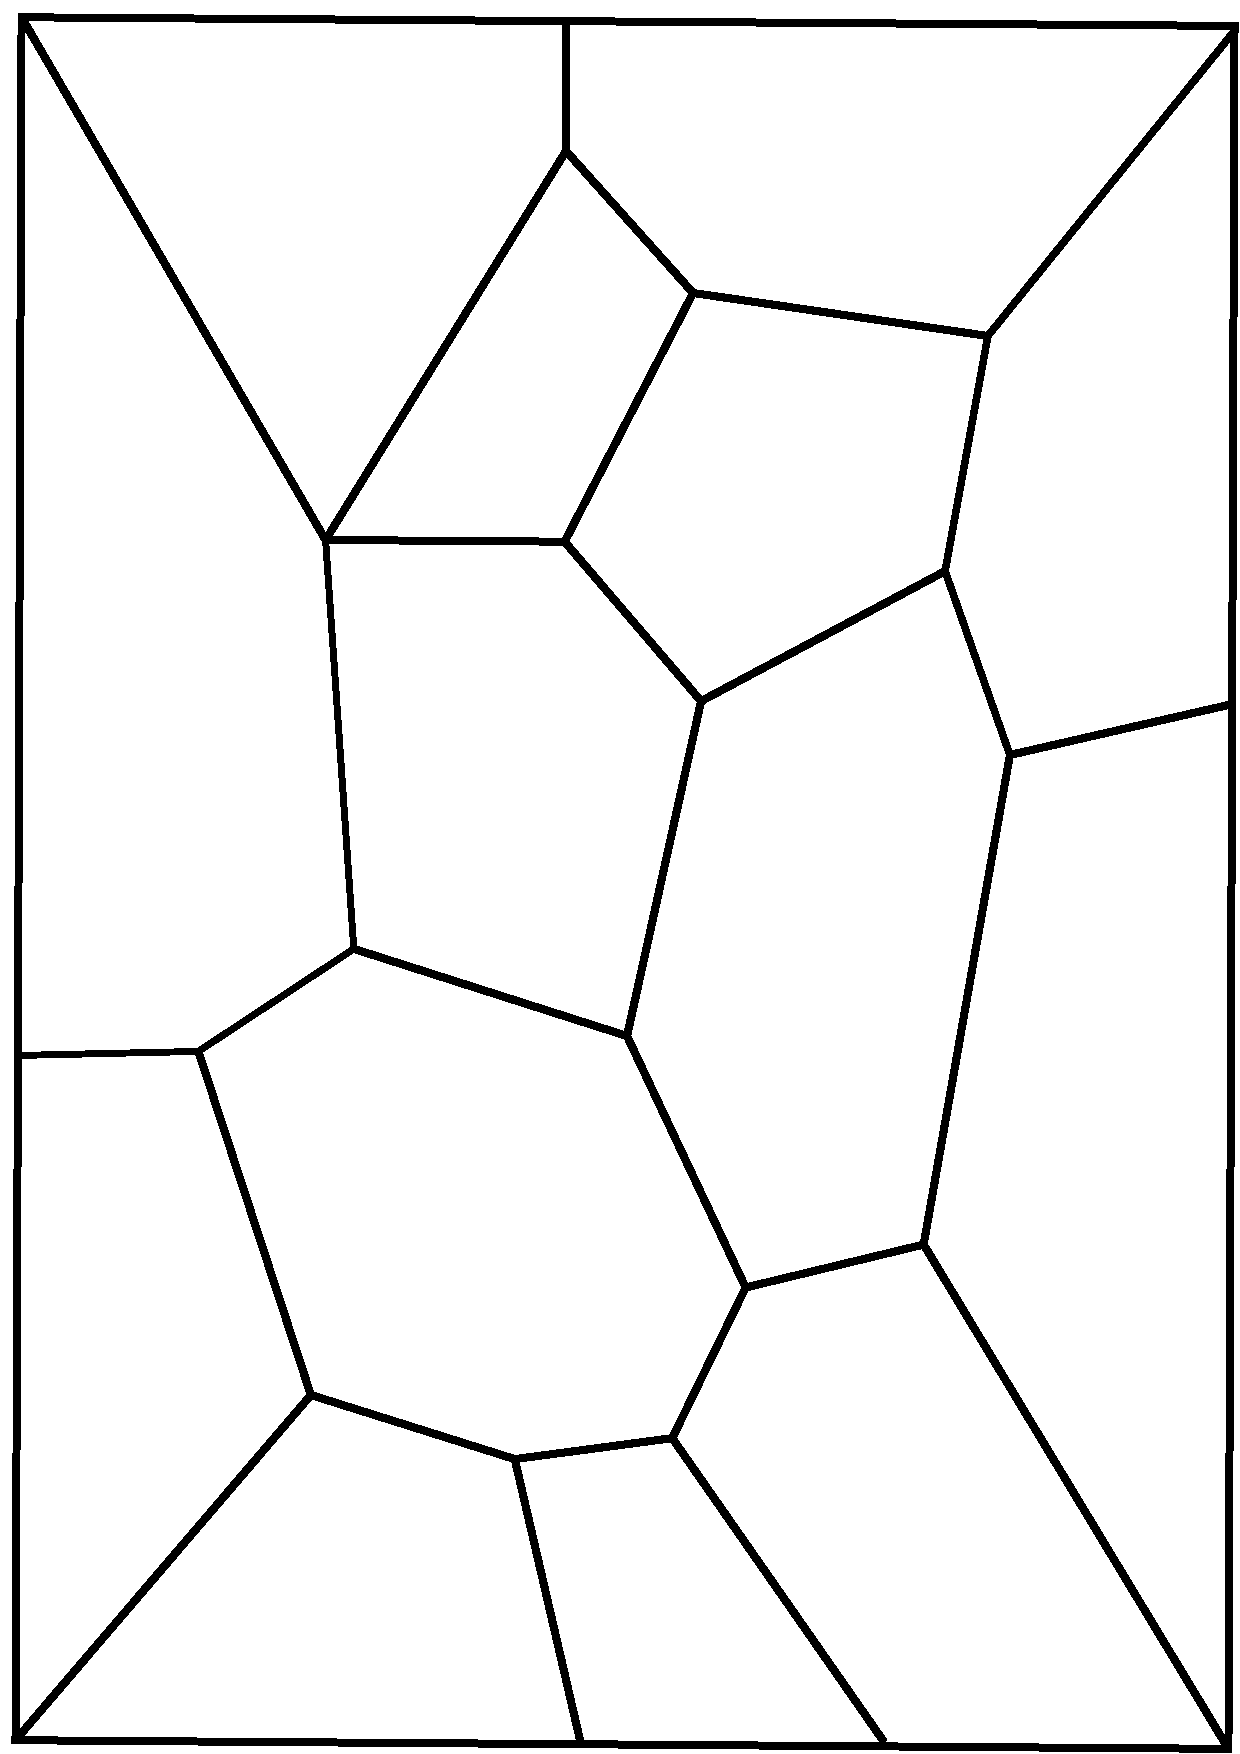
\includegraphics[width=70mm,height=70mm]{input_voronoi_cell_complex}
    \quad\quad
    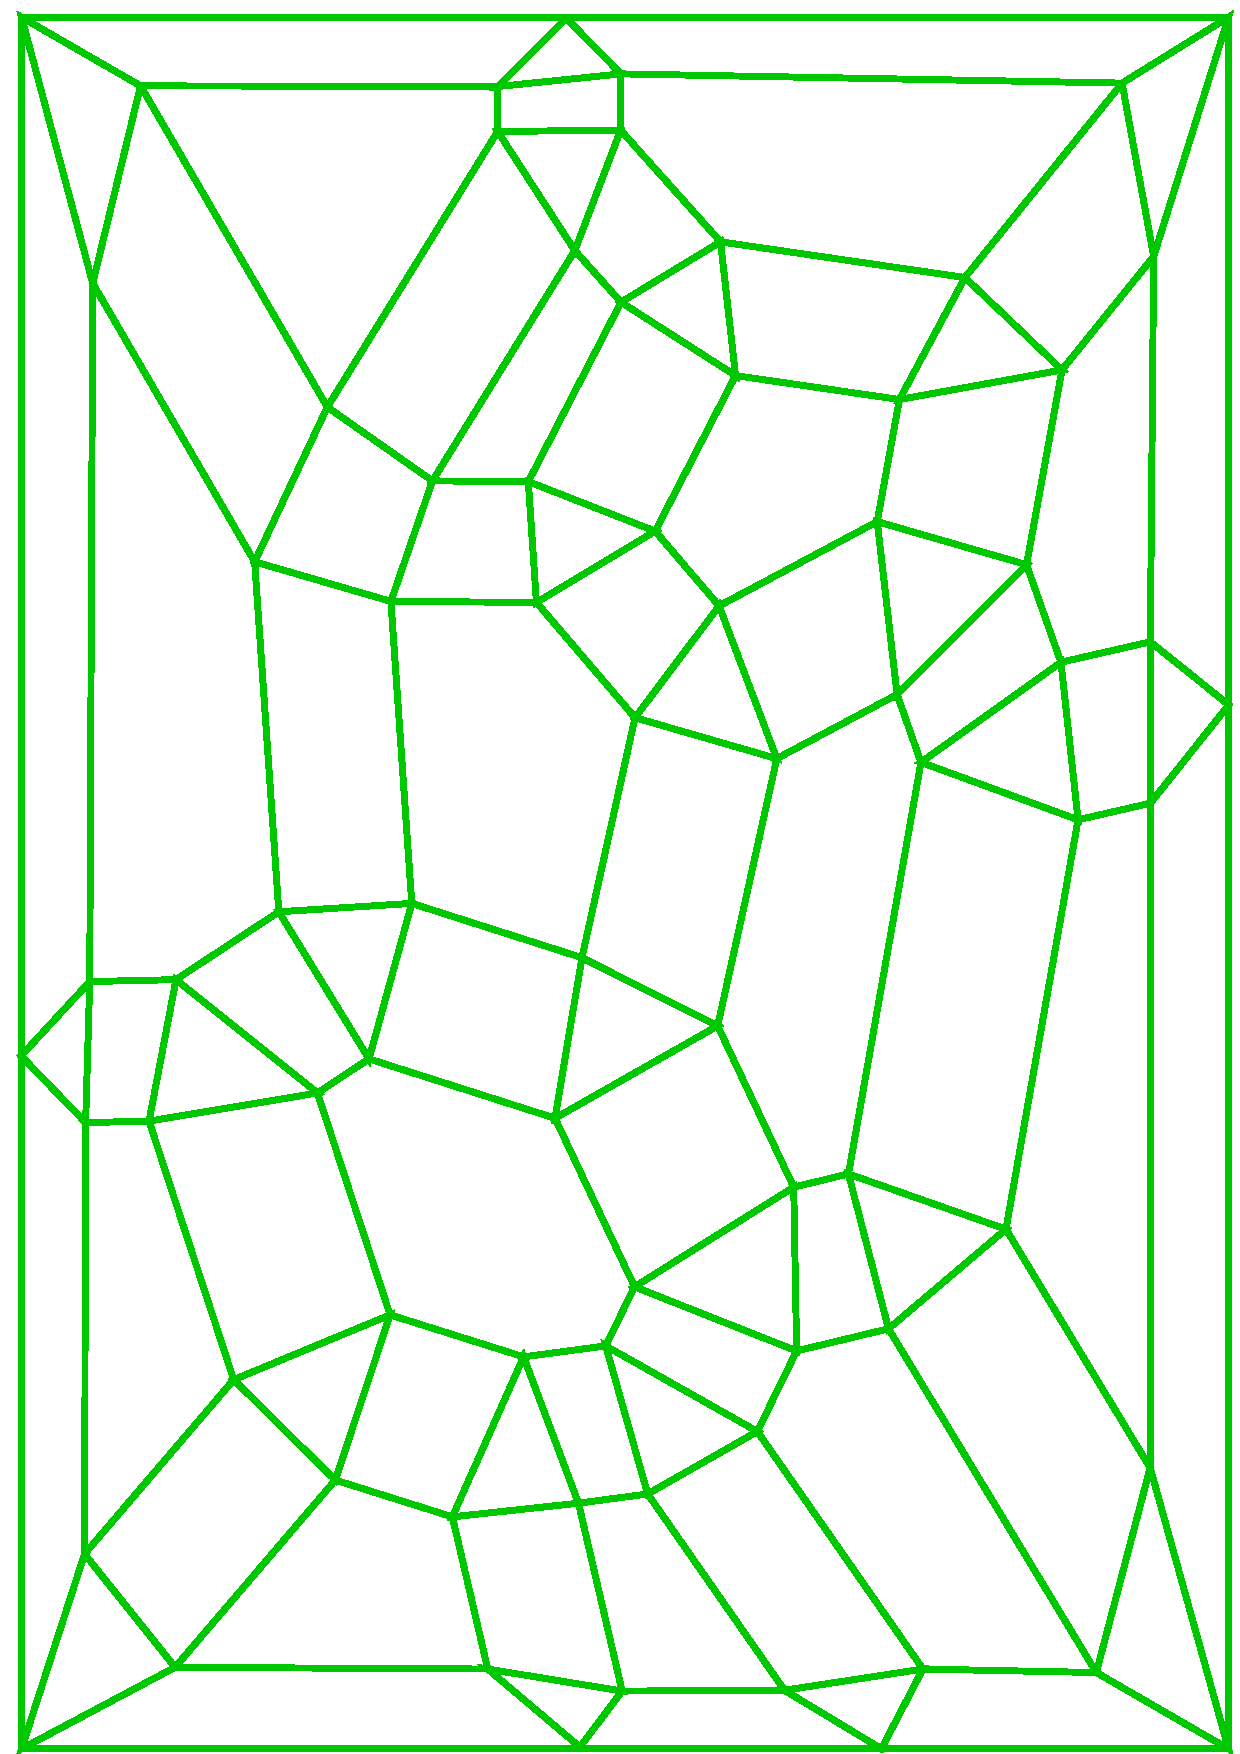
\includegraphics[width=70mm,height=70mm]{input_voronoi_cell_complex_transformation}
    \caption{
      A $2$-complex $K$ in the plane (left) and its Euler transformation $\hK$ (right).
      Every vertex in $\hK$ has degree $4$.
    }
    \label{fig:eulermeshillust}
\end{figure}

%\vspace*{-0.1in}
\section{Notations, Definitions on Polyhedral Complexes} \label{sec:defns}

We present definitions that we use to specify properties of the input complex $K$ as well as the Euler transformed complex $\hK$.
See standard books on algebraic topology \cite{Hatcher2002,Munkres1984} for details.
For quick reference, we collect important notation used throughout the paper in Table \ref{tab:notation}.


\begin{table}[h!]
  \centering
  \caption{\label{tab:notation} Notations used in the paper, and their explanations.}
  \begin{tabular}{ll}
    \hline
    Notation & definition/interpretation \\    \hline
    \vspace*{-0.1in} \\
    $K, \hK$     & input complex and its transformed complex \\
    $|K|$        & underlying space of complex $K$\\
    $\CO, \hCO$  & single $d$-cell defining the \emph{outside}, before and after transformation\\
    $\CH, \hCH$  & collection of $d$-cells defining holes, before and after transformation \\
    $v_i, e_i, f_i, t_i$ & (generic) vertex, edge, polygon ($2$-cell), and $3$-cell in $K$\\
    $\hv_i, \he_i, \hf_i, \htt_i$ & (generic) cells of dimensions 0--3 in $\hK$\\
    $\hf, \hf_e, \hf_v$ & Class-$1$, $2$, $3$ cells in $\hK$ in 2D \\
    $\htt, \htt_f, \htt_e, \htt_v$ & Class-$1$, $2$, $3$, $4$ cells in $\hK$ in 3D\\
    $V, E, F, T$ & set of vertices, edges, polygon ($2$-cells), and $3$-cells in $K$ \\
    $\hV, \hE, \hF, \hT$ & sets of vertices, edges, polygon ($2$-cells), and $3$-cells in $\hK$\\
    $\rho$, $D$ & inradius and diameter of a cell in $K$\\
    $\hrho$, $\hD$ & inradius and diameter of a cell in $\hK$\\ 
    $\gamma(f), \gamma(\hf)$ & aspect ratios of cells $f \in K, \hf \in \hK$ \\
    $\lambda$, $\mu$ & aspect ratio parameters for a particular edge $\hK$ \\
    $\lambda^*$, $\mu^*$ & parameters over all edges in $\hK$ \\
    $|e_{\min}|, |e_{\max}|$ & minimum and maximum edge length in a $2$-cell in $K$ \\
    $|\he_{\min}|, |\he_{\max}|$ & minimum and maximum edge length in a $2$-cell in $\hK$\\
    $\theta_{\min}$ & minimum interior angle of a $2$-cell in $K$ \\
    $\alpha, \beta$ & maximum and minimum angles formed by edges of $\hf_v$ on vertex $v$\\
    \hline
  \end{tabular}
\end{table}

\begin{defn} \label{def:plyhdcplx}
  \emph{\bfseries (Polyhedral complex)}
  A polyhedral complex (also called polytopal complex) $K$ is a collection of \emph{polyhedra} (polytopes) in some Euclidean space $\R^d$ such that every face of a polyhedron in $K$ is also included in $K$, and the nonempty intersection of any two polyhedra in $K$ is a face of both.
  The polyhedra in $K$ are referred to as its \emph{cells}.
  The \emph{dimension} $d$ of a polyhedral complex $K$ is the largest dimension of any cell in $K$.
  In this case, we refer to $K$ as a $d$-complex.
\end{defn}

We will work with \emph{finite} polyhedral complexes, i.e., when the set of cells in $K$ is finite.
While some of our definitions and results apply in arbitrary dimensions, we concentrate mostly on \emph{full-dimensional} polyhedral complexes of dimensions $2$ and $3$, i.e., in $\R^2$ and $\R^3$, respectively.
We will follow the convention that cells up to dimension $3$ are referred to as polyhedra (higher dimensional versions are termed \emph{polytopes}).
Formally, a $d$-dimensional polyhedron (a $d$-cell) is homeomorphic to the closed $d$-dimensional Euclidean ball.
The $d$-cells of interest in this work are vertices ($d=0$), edges ($d=1$), polygons ($d=2$), and \emph{polyhedra} or $3$-cells ($d=3$).

Our definition of Euler transformation (in \cref{sec:eulertsfm}) as well as geometric realization results in $d=2,3$ (in \cref{sec:geomrlzn}) do not require the polyhedra in $K$ to be convex.
Note that vertices and edges are always convex, but polygons and $3$-cells could be nonconvex in our general setting.
Further, some cells in the Euler transformed complex $\hK$ may not to be convex.
But if we assume cells in $K$ are convex, then we can guarantee a large majority of cells in $\hK$ are so as well.
We assume cells in $K$ are convex when describing results on the geometric quality of cells in $\hK$ (in \cref{sec:geomqual}).

\begin{defn} \label{def:purecplx}
  \emph{\bfseries (Pure  complex)}
  A polyhedral $d$-complex is \emph{pure} if every $p$-cell in $K$ for $p < d$ is a face of some $d$-cell in $K$.
\end{defn}
Being pure means that all top-dimensional cells in $K$ have dimension $d$.
A pure $2$-complex has no ``isolated'' edges or vertices, for instance.
In other words, every edge is a face of some polygon in the complex.

We assume the input mesh $K$ is a finite, connected, pure $d$-complex in $\R^d$ for $d=2$ or $d=3$.
Along with $K$, we assume we are given a collection $\CH$ of $d$-cells that capture $d$-dimensional \emph{holes}, and a singleton set $\CO$ that contains a $d$-cell capturing the \emph{outside}.
To be precise, $\CH = \cup_i c_i$ where each $c_i$ is a $d$-cell that is \emph{not} part of $K$ but all $(d-1)$-cells that constitute its $d$-boundary, which is homeomorphic to a $(d-1)$-sphere, are present in $K$.
Note that $p$-cells for $p < d$ in the intersection of a $d$-cell in $K$ and a $d$-cell in $\CH$ or $\CO$ are precisely the boundary cells of $K$.
For technical reasons that we explain later, we make the following assumptions about intersections of full-dimensional cells in $K$, $\CH$, and $\CO$.
We denote the \emph{underlying spaces} of these objects as $|K|, |\CH|$, and $|\CO|$, respectively.
Note that $|\CH| = \cup_{c_i \in \CH} |c_i|$.

\begin{asmn} \label{asmn:Kholesoutside}
  The following conditions hold for the input complex $K$, the collection of holes $\CH$, and the outside cell $\CO$.
  \begin{enumerate}
    \item $|K| \cup |\CH| \cup |\CO| = \R^d$.
    \item \label{asmn:sepholes} $d$-cells in $\CH$ are pairwise disjoint, and are also disjoint from the $d$-cell that is $\CO$. 
    \item \label{asmn:holeintr} Any $d$-cell in $K$ and a $d$-cell in $\CH$ intersect in at most \emph{one} $(d-1)$-facet of both. See \cref{rem:adjbdyedges} for an explanation of the need for this assumption.
    \item  \label{asmn:outintr} No two $(d-1)$-cells that are \emph{adjacent facets} of a $d$-cell in $K$, i.e., they intersect in a common $(d-2)$ cell, intersect the $d$-cell that is $\CO$. Again, see \cref{rem:adjbdyedges} for an explanation.
  \end{enumerate}
\end{asmn}
%
\noindent Intuitively, the $d$-cells in $K, \CH$, and $\CO$ cover all of $\R^d$, and each $d$-cell in $\CH$ captures a separate hole that is also separate from the outside.

We point out that \emph{articulation} (or cut) vertices are allowed in $K$, i.e., vertices whose removal disconnects the complex (we assume $K$ is connected to start with).
Conditions specified in \cref{asmn:Kholesoutside} ensure such vertices are boundary vertices of $K$.
For instance, $K$ could consist of two copies of the complex shown on the left in \cref{fig:eulermeshillust} that meet at one of the four corner points.


\section{Definition of Euler Transformation} \label{sec:eulertsfm}

We define the Euler transformation $\hK$ of the input $d$-complex $K$ by explicitly listing the $d$-cells that are included in $\hK$.
Since we are working with cells (rather than simplices), we specify each $d$-cell by explicitly listing all $(d-1)$-cells that are its facets.
We denote vertices as $v$ (or $u, v_i$), edges as $e$ (or $e_i$), polygons or $2$-cells as $f$ (or $f_i$), and $3$-cells as $t$ (or $t_i$).
The corresponding cells in $\hK$ are denoted $\hv, \he, \hf, \htt$, and so on.
We first define the cells in $\hK$ \emph{abstractly}, and discuss aspects of geometric realization in \cref{sec:geomrlzn}.

\vspace*{-0.05in}
\subsection{Euler transformation for $d=2$} \label{ssec:euler2d}
\vspace*{-0.05in}

We start by \emph{duplicating} every polygon ($2$-cell) in $K \cup \CH \cup \CO$.
Since we do not want to alter the domain in $\R^d$ captured by $K$, we set $\hCH = \CH$ and $\hCO = \CO$.
But we ``shrink'' each polygon in $K$ when duplicating (see \cref{sec:geomrlzn} for details).
By the definition of $K$ and \cref{asmn:Kholesoutside}, this duplication results in each edge $e \in K$ being represented by two copies in $\hK$.

The polygons ($2$-cells) in $\hK$ belong to three classes, and correspond to the polygons, edges, and vertices in $K$ as described below.
See Figure \ref{fig:3types2cells2d} for illustrations of each class.
\begin{enumerate}
  \item \label{2dETcls1}
    For each polygon $f \in K$, we include $\hf \in \hK$ as the copy of $f$.

  \item \label{2dETcls2}
    Each edge $e \in K$ generates the $4$-gon ($4$-sided polygon) $\hf_e$ in $\hK$ specified as follows.
    Let $e = \{u,v\} \in f,f'$, where $f \in K$ and $f' \in K \cup \CH \cup \CO$.
    Then $\hf_e$ is the polygon whose facets are the four edges $\{\hu,\hv\}, \, \{\hv,\hv'\}, \, \{\hu',\hv'\}$, and $\{\hu,\hu'\}$.
    Here, $\hv, \hv'$ are the two copies of $v$ in $\hK$.
    Note that the edges $\he = \{\hu,\hv\}$ and $\he' =  \{\hu',\hv'\}$ are facets of the Class \ref{2dETcls1} polygons $\hf$ added to $\hK$ (as described above) or of the polygons $\hf'$ in $\hCH$ or $\hCO$.
    Edges $\{\hu,\hu'\}$ and $\{\hv,\hv'\}$ are added new.
    
  \item \label{2dETcls3}
    Each vertex $v \in K$ that is part of $p$ polygons in $K$ generates a $p$-gon (polygon with $p$ sides) $\hf_v$ in $\hK$ whose vertices and edges are specified as follows.
    Let $v \in f_k$ for $k=1,\dots,p$ in $K$.
    Then $\hf_v$ has vertices $\hv_k$, $k=1,\dots,p$, where $\hv_k$ is the copy of $v$ in $\hf_k$ (in $\hK$).
    For every pair of polygons $f_i,f_j \in \{f_k\}_1^p$ that intersect in an edge $e_{ij} \in K$, the edge $\he_{ij} = \{\hv_i, \hv_j\}$ is included as a facet of $\hf_v$.
    Note that edges $\he_{ij}$ are precisely the edges added new as facets of the Class \ref{2dETcls2} polygons described above.
\end{enumerate}
%
\begin{figure}[htp!]
  \centering
  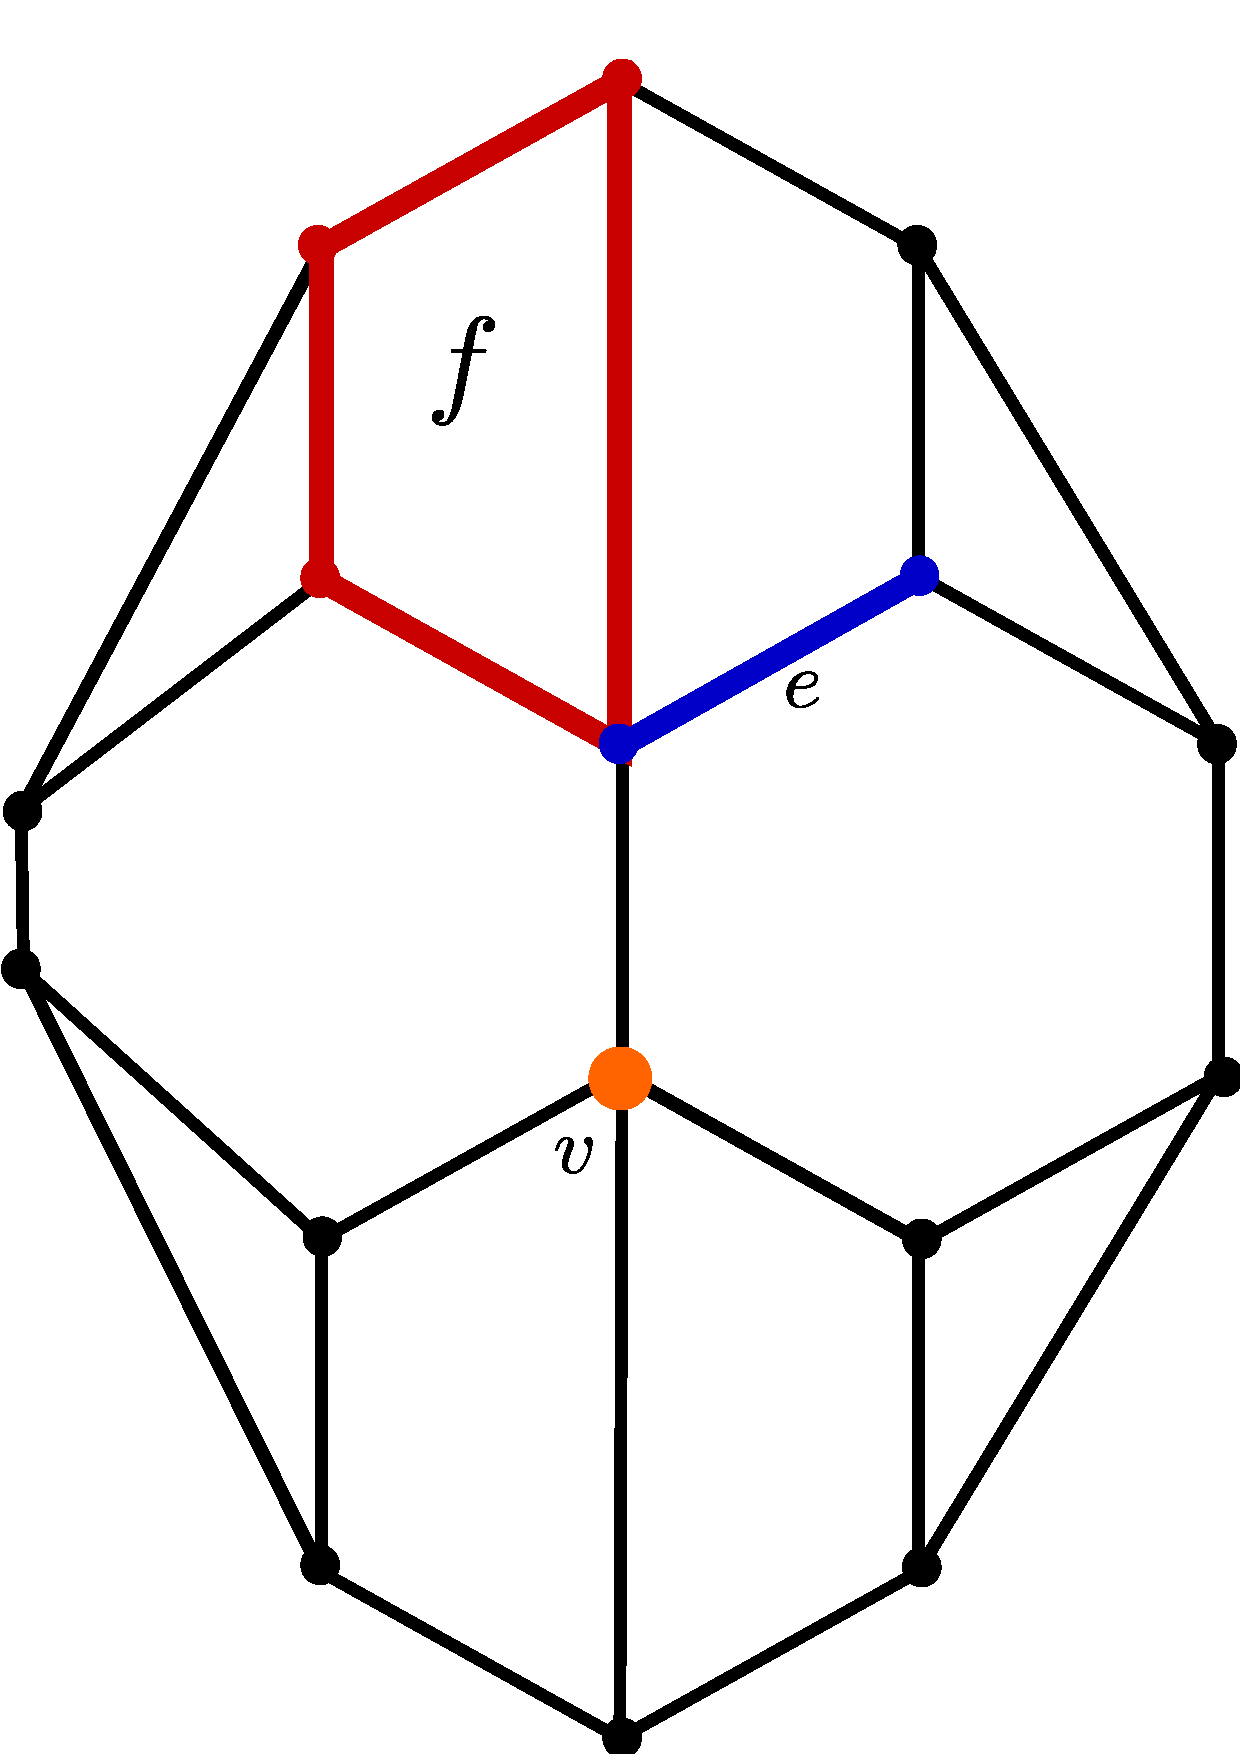
\includegraphics[scale=0.2]{input_complex}
  \quad
  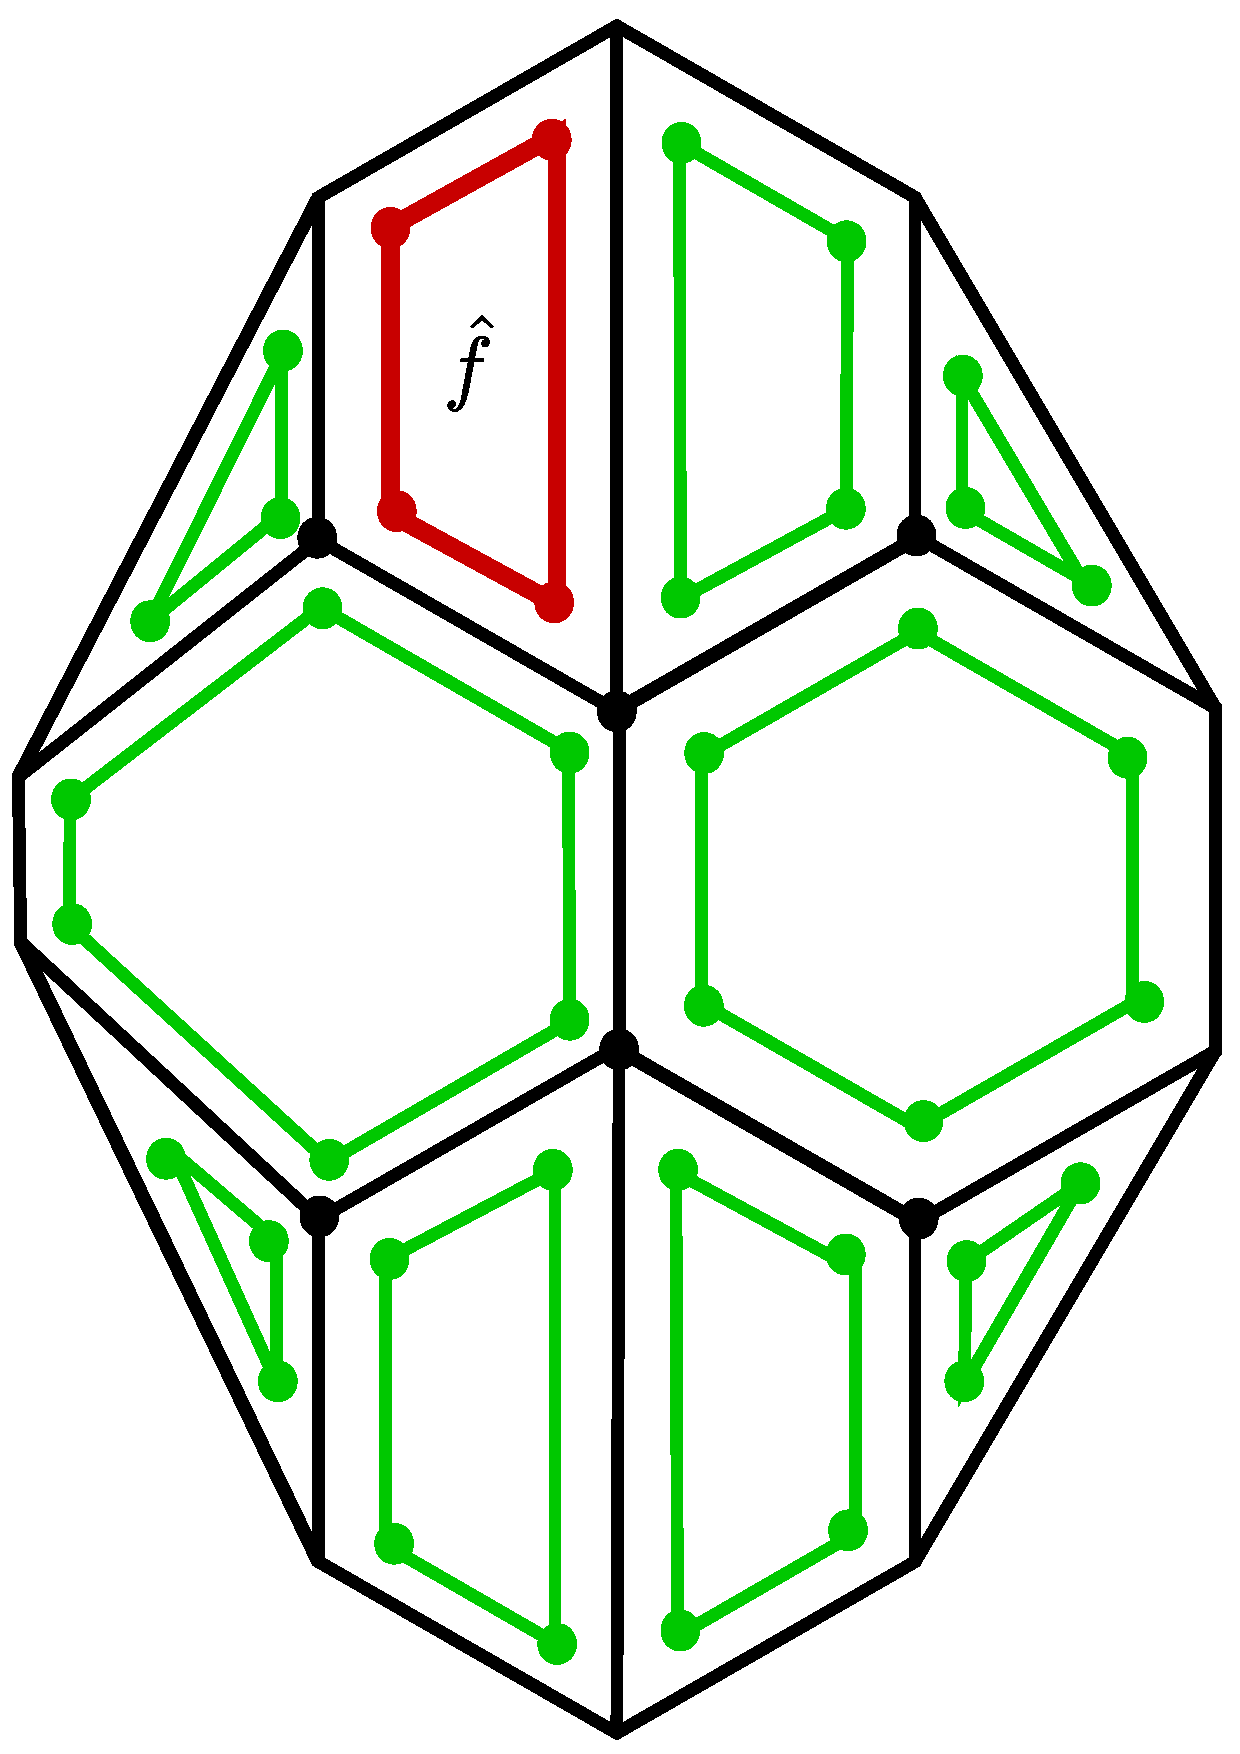
\includegraphics[scale=0.2]{vertices_offset_new_complex.pdf}
  \quad
  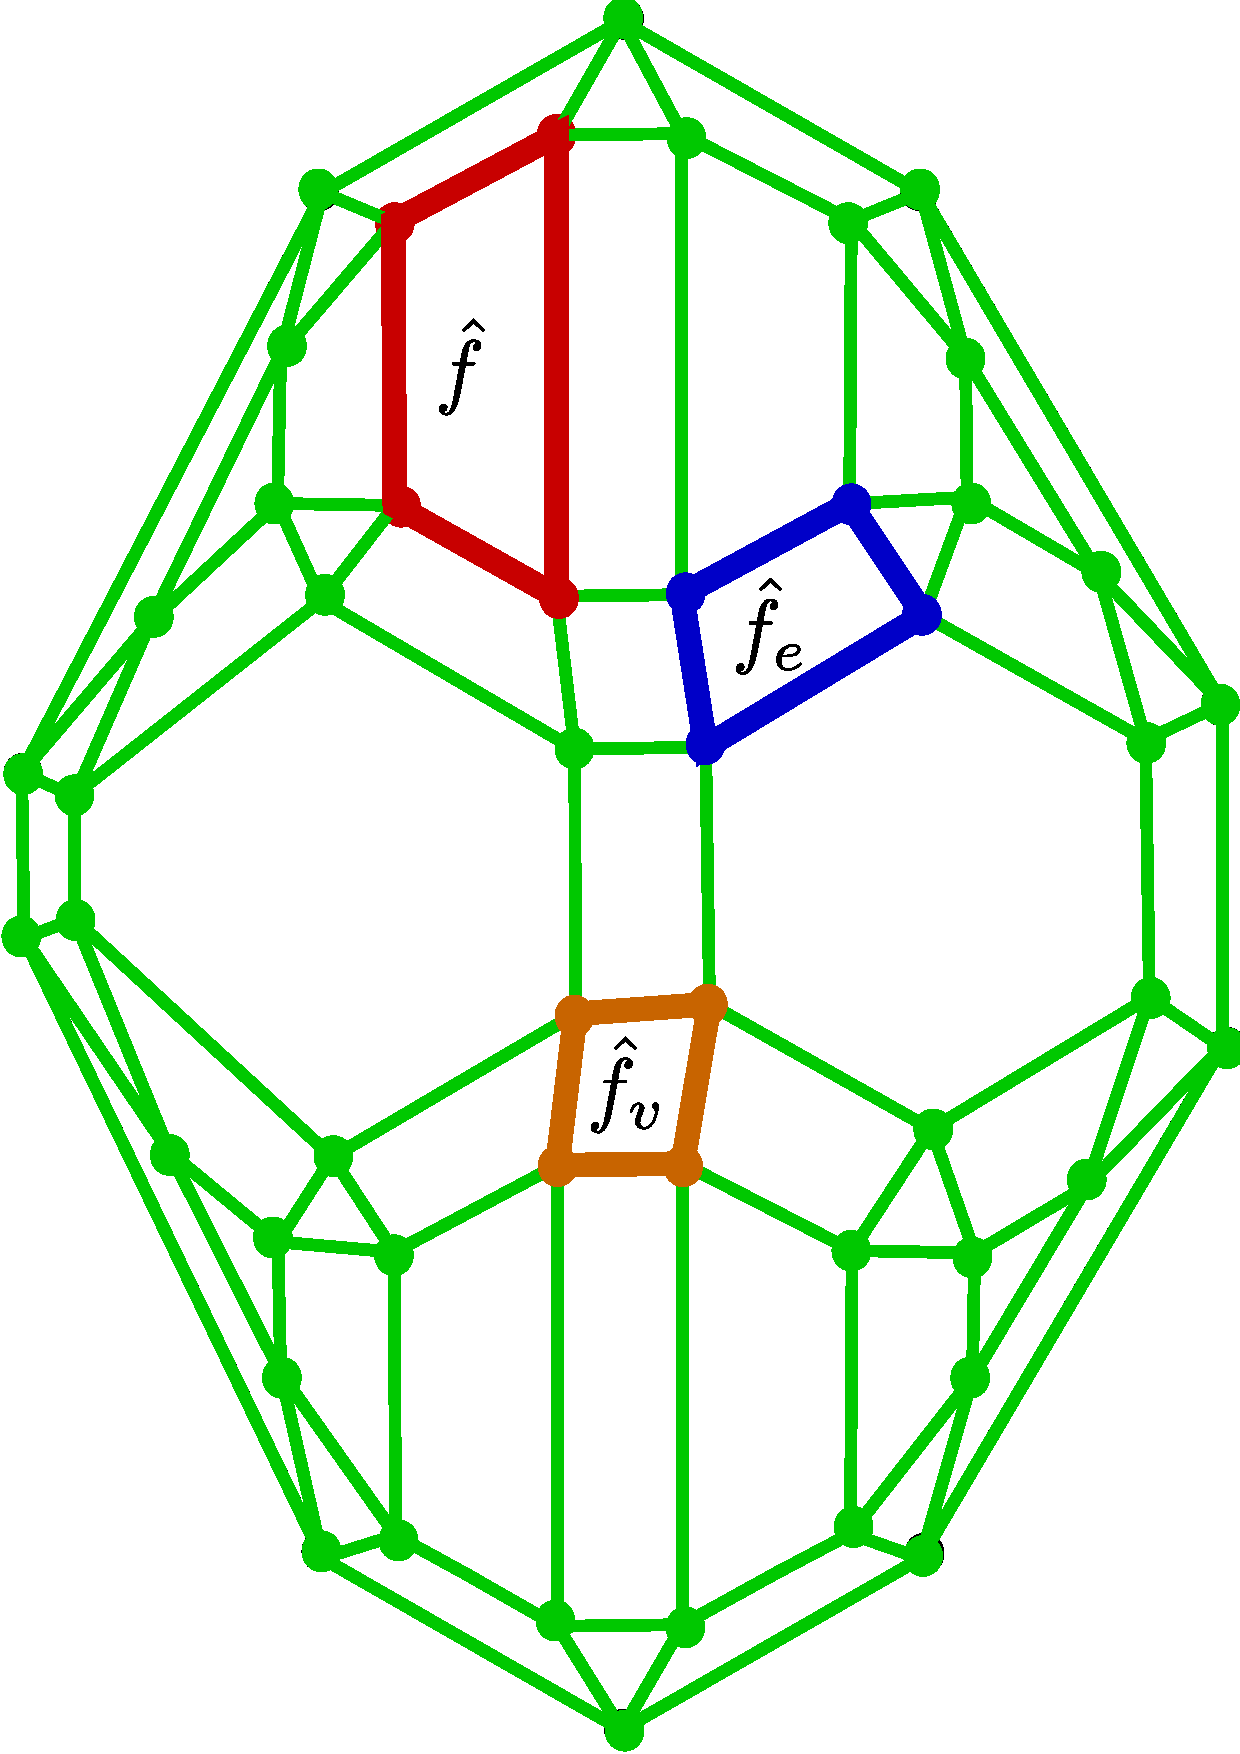
\includegraphics[scale=0.2]{edges_new_complex}
  \caption{A polygon $f$, edge $e$, and a vertex $v$ highlighted in an input complex $K$ (left),
    an intermediate complex showing only the copies of original polygons in $K$ that are included in $\hK$, i.e., of Class \ref{2dETcls1} (middle),
    and the final Euler transformation $\hK$ (right).}
  \label{fig:3types2cells2d}
\end{figure}


\subsection{Euler transformation for $d=3$} \label{ssec:euler3d}

We start by duplicating every polyhedron ($3$-cell) in $K \cup \CH \cup \CO$.
Similar to the case of $d=2$, we set $\hCH = \CH$ and $\hCO = \CO$, but ``shrink'' each $3$-cell in $K$ when duplicating.
This duplication results in each polygon $f \in K$ being represented by two copies in $\hK$.

The $3$-cells in $\hK$ belong to four classes, and correspond to the $3$-cells, polygons, edges, and vertices in $K$ as described below.
%
%\clearpage
\begin{enumerate}
  \item \label{3dETcls1}
    For each $3$-cell $t \in K$, we include $\htt \in \hK$ as the copy of $t$.
    
  \item \label{3dETcls2}
      Each $p$-sided polygon $f \in K$ generates a $3$-cell $\htt_f$ in $\hK$ with $p+2$ polygons as facets specified as follows.
      Let $f$ be a facet of $3$-cells $t, t'$ where $t \in K$ and $t' \in K \cup \CH \cup \CO$.
      Also, let $f$ consist of vertices $\{v_i\}_{i=1}^p$ and edges $e_i=\{v_i,v_j\}$ for $i=1,\dots,p-1,\,j=i+1$ and $i=p,j=1$.
      Then the polygons that are facets of $\htt_f$ include $\hf, \hf'$, and the $p$ $4$-gons $\hf_i$ whose edges consist of $\he_i,\he'_i, \{\hv_i,\hv_i'\}, \{\hv_j, \hv_j'\}$ for $i=1,\dots,p-1,\,j=i+1$ and $i=p,j=1$.
      Here, $\hv'_i, \he'_i$ are the vertex and edge in $\hf'$ generated by $v_i, e_i$ for each $i$, where $\hf'$ is the polygonal facet of $\htt'$ corresponding to $f$.
      And $\htt'$ is the Class \ref{3dETcls1} $3$-cell in $\hK$ (as defined above) corresponding to $t'$.

      We also note that the polygons $\hf,\hf'$ are already included as facets of $\htt, \htt'$, which are added to $\hK$ as Class \ref{3dETcls1} cells.
      The vertices $\hv_i, \hv'_i$ are included already as part of $\htt, \htt'$ as well.
      The $p$ $4$-gons $\hf_i$ are added \emph{new}, and so are the edges $\{\hv_i,\hv'_i\}$ for $i=1,\dots,p$.
      See Figure \ref{fig:3dETcls2} for an illustration with $p=5$.
      \begin{figure}[htp!]
        \centering
        %\vspace*{-0.1in}
        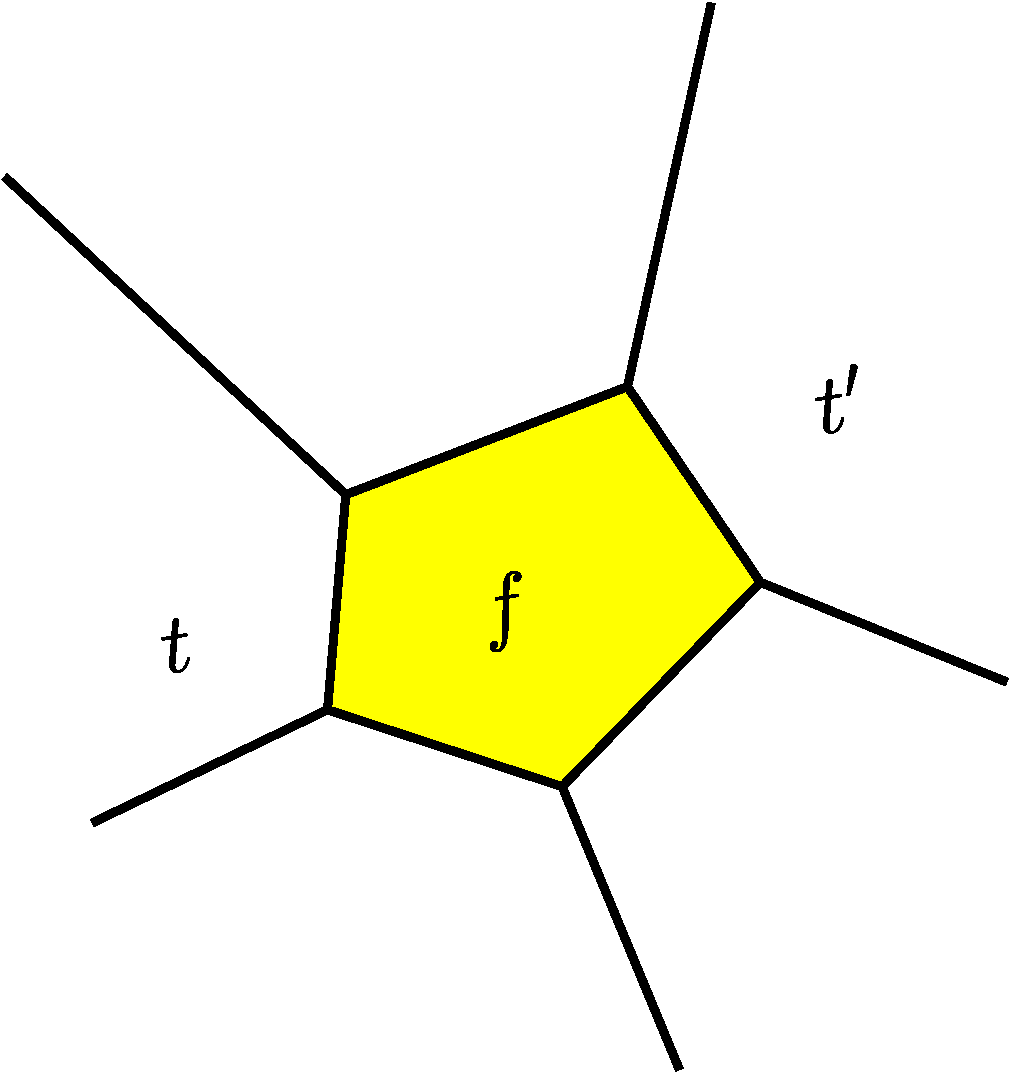
\includegraphics[scale=0.2]{euler_transformation_3d_across_face_input-crop}
        \hspace*{0.3in}
        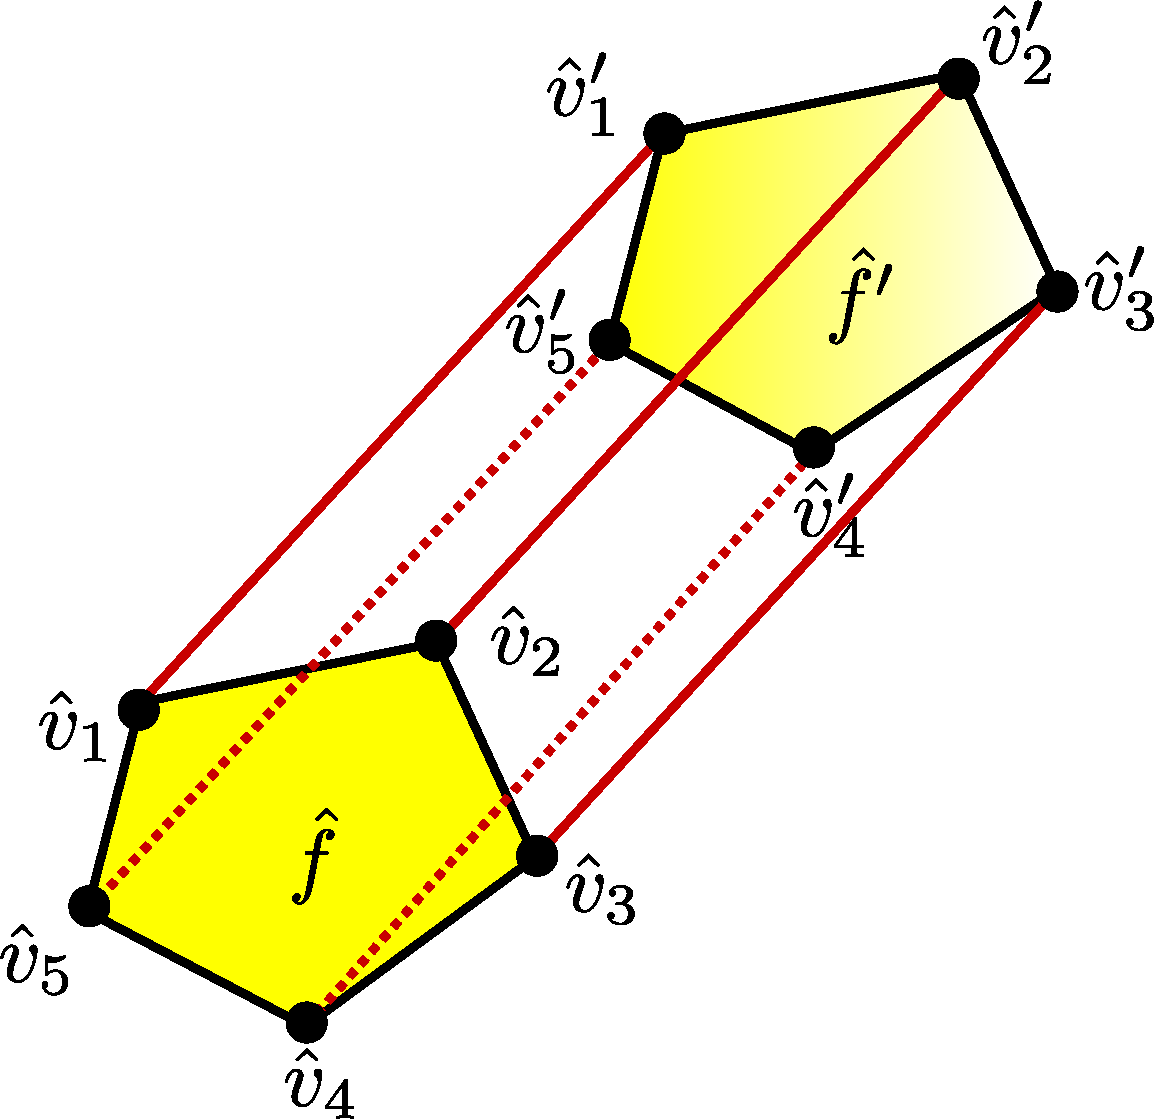
\includegraphics[scale=0.2]{euler_transformation_3d_across_face_ouput-crop}
        \caption{Illustration of a Class \ref{3dETcls2} $3$-cell $\htt_f$ (right) generated by the pentagon $f \in K$ (left).
          The $p=5$ $4$-gons are not shaded for clarity.}
        \label{fig:3dETcls2}
      \end{figure}
      %\vspace*{-0.1in}
      
  \item \label{3dETcls3}
    Each edge $e \in K$ that is part of $q$ $3$-cells generates a $3$-cell $\htt_e$ in $\hK$ with $q+2$ polygons as facets specified as follows.
    Let $\{t_i\}_{i=1}^q$ be the $q$ $3$-cells that have $e = \{u,v\}$ as an edge, and
    let $\he_i = \{\hu_i, \hv_i\},\,i=1,\dots,q$ be the $q$ copies of the edge $e$ in $\htt_i$.
    We add a $4$-gon $\hf_i$ as a facet of $\htt_e$ for every pair of \emph{adjacent} $3$-cells $t_i,t_j$ from this collection, i.e., when $t_i \cap t_j = f_{ij}$ is a polygon that contains $e$ as an edge, for $i=1,\dots,q-1,\,j=i+1$ and $i=q,j=1$.
    The edges of this $4$-gon $\hf_i$ are $\he_i, \he_j, \{\hu_i, \hu_j\}$, and $\{\hv_i, \hv_j\}$.
    Note that there are $q$ such $4$-gons $\hf_i$ that are facets of $\htt_e$.
    Also note that these $4$-gons are already included as faces of the Class \ref{3dETcls2} $3$-cells $\htt_{f_{ij}}$ described above.

    Finally, we add two \emph{new} $q$-gons as facets of $\htt_e$ whose $q$ edges are $\{\hu_i,\hu_j\}$ and $\{\hv_i,\hv_j\}$, respectively, for  $i=1,\dots,q-1,\,j=i+1$ and $i=q,j=1$.
    \cref{fig:3dETcls3} illustrates a $q=5$ instance.
    At the same time, these $q$-gons cannot be guaranteed to be planar in all geometric realizations of $\hK$ (see \cref{rem:nonplnr3d}). % in \cref{ssec:rlzn3d}).
    \begin{figure}[htp!]
      \centering
      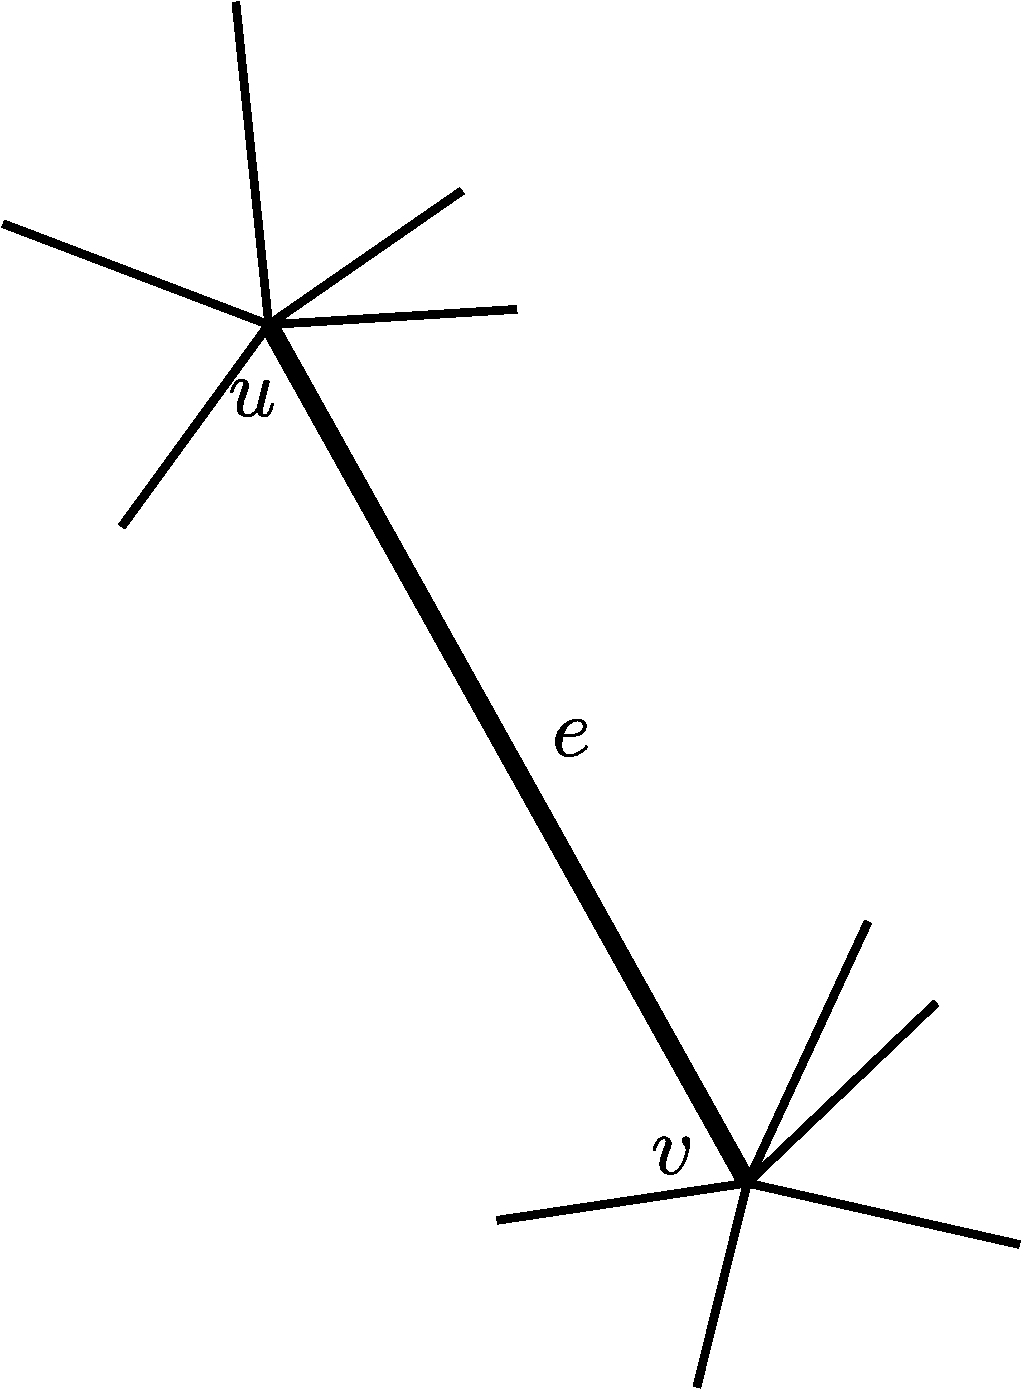
\includegraphics[scale=0.2]{euler_transformation_3d_around_edge_input-crop.pdf}
      \hspace*{0.1in}
      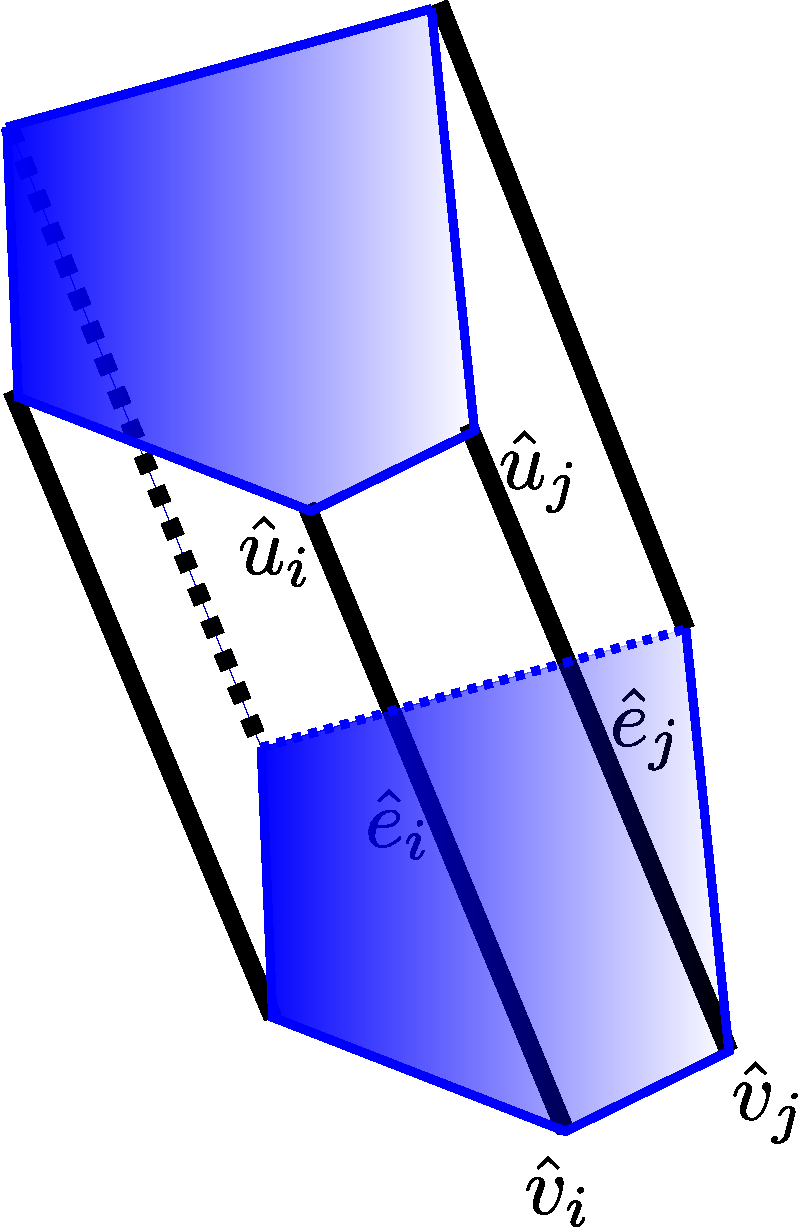
\includegraphics[scale=0.2]{euler_transformation_3d_around_edge_output-crop.pdf}
      \caption{Illustration of a Class \ref{3dETcls3} $3$-cell $\htt_e$ (right) generated by the edge $e \in K$ shared by $5$ cells (left).
        The $q=5$ $4$-gons are not shaded for clarity.
      }
        \label{fig:3dETcls3}
    \end{figure}

  \item \label{3dETcls4}
    Each vertex $v \in K$ generates a $3$-cell $\htt_v$ in $\hK$ specified as follows.
    Let $v$ be a vertex in $r$ $3$-cells $\{t_k\}_{k=1}^r$, and let $\hv_k$ be the corresponding copy of $v$ in $\htt_k$ (in $\hK$) for $k=1,\dots,r$.
    Then the vertices of $\htt_v$ are precisely $\hv_1,\dots,\hv_r$.
    For every pair of \emph{adjacent} $3$-cells $t_i,t_j \in \{t_k\}_{k=1}^r$, i.e., when $t_i \cap t_j$ is a polygon that contains $v$ as a vertex, we add the edge $\{\hv_i,\hv_j\}$ to $\htt_v$.

    We then consider every subset $\sT \subset \{t_k\}_{k=1}^r$ of $3$-cells that intersect in an edge that has $v$ as one vertex.
    We add a polygon as a facet of $\htt_v$ that has as edges $\{\hv_i,\hv_j\}$ where $t_i,t_j \in \sT$ intersect in a polygon.
    We repeat this process for every such $\sT \subset \{t_k\}_{k=1}^r$ with $3 \leq |\sT| < r$.
    Note that each such polygon has already been added as a facet of the Class \ref{3dETcls3} $3$-cell generated by the edge common to the $3$-cells in collection $\sT$ (these are the $q$-gons described above).

\end{enumerate}

\begin{rem}
  Based on our definition of $\hK$, any two cells in $\hK$ intersect in a face of both cells, and all faces of cells are included in $\hK$.
  Hence $\hK$ is a polyhedral complex.
\end{rem}

\vspace*{-0.3in}
\begin{rem}
 \cref{thm:deg4ET2d}, \cref{lem:cntshVhEhF2d}, \cref{thm:deg6ET3d}, and \cref{lem:cntshThVhEhf3d} hold independent of the geometric realization of the Euler transformed complex.
\end{rem}


\section{Geometric Properties of the Euler Transformed Complex} \label{sec:geomrlzn}

As Euler transformation adds new full-dimensional cells corresponding to polygonal facets, edges, and vertices, we \emph{offset} the cells added to $\hK$ as copies of the full-dimensional cells in $K$ in order to generate enough space to add the extra cells.
Intuitively, we ``shrink'' each of the full-dimensional cells in $K$ in order to produce cells in $\hK$ that are geometrically similar to the input cells.
We use standard techniques for producing offset polygons in 2D, e.g., \emph{mitered offset} generated using the straight skeleton (SK) of the input polygon \cite{AiAuAlGa1995}.
For the sake of completeness, we include the definition of mitered offset.

 \vspace*{-0.3in}
 \begin{defn} \label{def:miteredoffset}
      \emph{\bfseries (Mitered offset \cite{AiAuAlGa1995})}
      The mitered offset of a polyhedron $P$ with offset distance $b$ is the polyhedron obtained by moving each facet of $P$ toward its interior in a self parallel manner by distance $b$. 
 \end{defn}

For the $d=2$ case, we define the cell offset as a mitered offset of the polygon (i.e., choice of $b$ in \cref{def:miteredoffset}) that creates no \emph{combinatorial} or \emph{topological changes}---i.e., no edges are shrunk to points, and the polygon is not split into multiple polygons.
On the other hand, we have studied the case of mitered offset with \emph{combinatorial} or \emph{topological changes} in $d=2$ separately \cite{GuKrDr2020}.

Unlike for polygons, parallel offsetting of a polyhedron ($d=3$) is not defined uniquely in general \cite{BaEpGoVa2008}.
Although a unique offset polyhedron could be constructed for orthogonal polyhedra or for convex polyhedra \cite{BaEpGoVa2008,MaViPl2011}, shrinking a generic polyhedron goes through continuous geometrical changes, combinatorial changes, as well as topological changes (e.g., breaking into multiple polyhedra).
In fact, offsetting vertices with degree $4$ or more in the $1$-skeleton of the polyhedron can produce multiple vertices even with an infinitesimal shrinkage \cite{AuWa2013,AuWa2016}.
Hence we assume in the case of $d=3$ that each vertex in the input cell complex $K$ has degree $3$ in the $1$-skeleton of each cell that it is part of, on top of the requirements in \cref{asmn:Kholesoutside}
(see \cref{rem:3dETdeg4vtx} for how one may deal with a complex where this assumption does not hold).
Under this assumption, we define the cell offset of a polyhedron as a mitered offset that creates no combinatorial or topological changes (similar to the case of polygons in $d=2$).

Naturally, we do not want to alter the domain modeled by the cell complex $K$, i.e., its underlying space $|K|$.
Hence we maintain the cells in $\CH$ and $\CO$, i.e., these cells are included in $\hK$ without any changes.
Since every top-dimensional cell is offset, the new cells in $\hK$ are \emph{fit} within the extra space created by offsetting each top-dimensional cell.

\subsection{Geometric Realization in $d=2$} \label{ssec:rlzn2d}

  \addtocounter{thm}{-1}

We state and prove several properties of the geometric realization of the Euler transformed polygon complex $\hK$ in $d=2$.
\add{We restrict our discussion to the cases where $2$-cells in $\hK$ are planar and edges are straight lines.}
We start with the main result---every vertex in $\hK$ has degree $4$ in its $1$-skeleton.

\begin{thm} \label{thm:deg4ET2d}
  Every vertex in $\hK$, the Euler transformation of the $2$-complex $K$, has degree $4$ in the $1$-skeleton of $\hK$.
\end{thm}
\begin{proof}
  Consider a vertex $v$ shared by adjacent edges $e_1, e_2 \in f$, where $f \in K \cup \CH \cup \CO$ is a polygon.
  Following \cref{asmn:Kholesoutside}, the edges $e_1$ and $e_2$ are shared by exactly two cells each from the input complex,  holes, or the outside cell.
  Let $f'_1, f'_2$ be the other polygons containing edges $e_1, e_2$, respectively (with $f$ being the first polygon).

  Consider the vertex $\hv \in \hK$ generated as part of $\hf$, as specified in the Euler transformation (\cref{ssec:euler2d}).
  $\hf$ is a mitered offset of $f$ when $f \in K$, or is identical to $f$ when it belongs to $\CH \cup \CO$.
  Hence $\hf$ is a simple polygon in both cases, and $\hv$ is part of two edges $\he_1, \he_2 \in \hf$.
  Further, $\hv$ will be part of two more edges $\{\hv,\hv'_1\}$ and  $\{\hv,\hv'_2\}$  added as facets of the Class \ref{2dETcls2} polygons generated by $e_1, e_2$.
  Here $\hv'_i \in \he'_i \in \hf'_i$ for $i=1,2$.
  Hence $\hv$ has degree $4$ in the $1$-skeleton of $\hK$.
\end{proof}


\begin{rem}
  \label{rem:adjbdyedges}
  {\rm 
    We show why we require the input complex to satisfy Conditions \ref{asmn:holeintr} and \ref{asmn:outintr} in \cref{asmn:Kholesoutside}, which require that no two adjacent edges of a polygon in $K$ can be boundary edges.
    Consider the input complex $K$ consisting of a single square, whose four edges are shared with the outside cell $\CO$.
    If we apply the Euler transformation as specified in \cref{ssec:euler2d}, every vertex in the output complex  $\tilde{K}$ will have the odd degree of $3$, as shown in Figure \ref{fig:outintr}.
    But if we apply the Euler transformation \emph{once more} to $\tilde{K}$, we do get a valid complex $\hK$ with each vertex having degree $4$.
    Note that $\tilde{K}$ does satisfy Condition \ref{asmn:outintr}, and hence becomes a valid input.
    \begin{figure}[htp!]
      \centering
      
\includegraphics[scale=0.2]{euler_transformation_twice_input-crop}
      \quad
      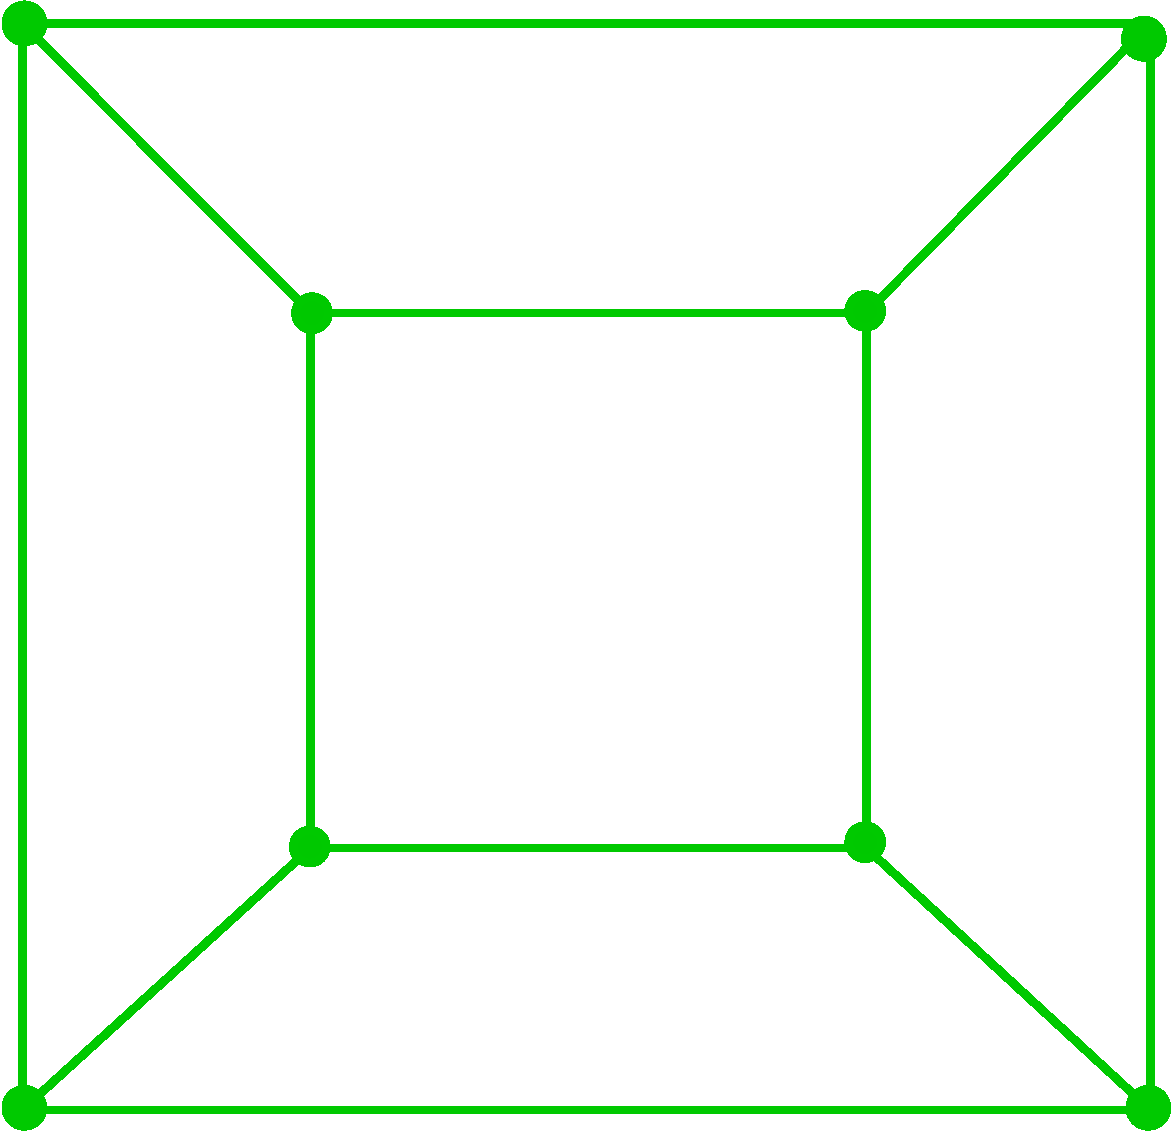
\includegraphics[scale=0.2]{euler_transformation_once-crop}
      \quad
      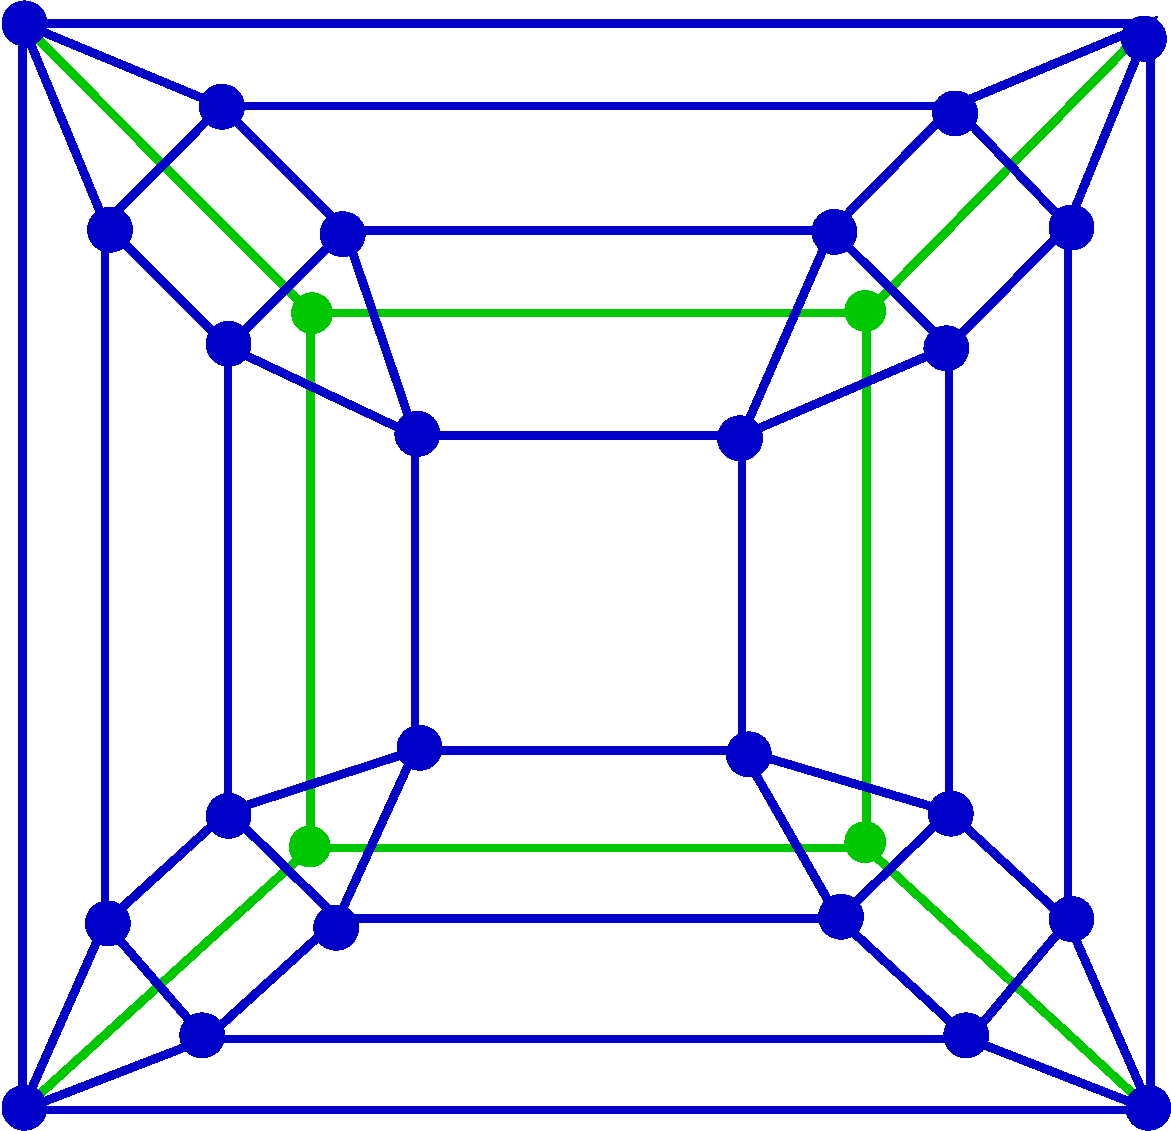
\includegraphics[scale=0.2]{euler_transformation_twice_finaloutput-crop}
      \caption{Applying the Euler transformation to the square $K$ whose more than one adjacent edge is shared with the outside (left) produces a complex $\tilde{K}$ in which every vertex has odd degree (middle).
      Applying the Euler transformation again to $\tilde{K}$ produces a valid complex $\hK$ where every vertex has degree $4$ (right).}
      \label{fig:outintr}
    \end{figure}
  }
\end{rem}

\begin{lem}
  \label{lem:cntshVhEhF2d}
  Let $V, E, F$ denote the sets of vertices, edges, and polygons (faces) in $K$, and let $\hV, \hE, \hF$ denote the corresponding sets in $\hK$.
  The following relations hold for the cardinalities of these sets: $|\hV| = 2|E|,~|\hE| = 4|E|$, and $|\hF| = |V| + |E| + |F|$.
\end{lem}

\begin{proof}
  Let $\delta(v)$ denote the degree of vertex $v \in K$, and let $\hf_v$ be the polygon generated by $v$ in $\hK$.
  This is a polygon of Class \ref{2dETcls3} specified in the definition of Euler transformation for $d=2$ (Section \ref{ssec:euler2d}).
  Following \cref{asmn:Kholesoutside} about $K, \CH, \CO$, it is clear that when $v$ belongs to $p$ polygons in $K$, we must have $\delta(v)=p$ and $\hf_v$ has $p$ vertices.
  Since each cell $\hf$ corresponding to polygon $f \in K$ is a mitered offset, and since each vertex $\hv$ is part of one such offset polygon, it follows that $\hf_u \cap \hf_v = \emptyset$ for any two vertices $u,v \in K$.
  Hence we get
  \[
    |\hV| = \sum_{v \in K} \delta(v) = 2|E|.
  \]
  %
  By \cref{thm:deg4ET2d}, each vertex $\hv \in \hK$ has degree $\hat{\delta}(\hv) = 4$ in $\hK$.
  Combined with the result above on $|\hV|$, we get that
  \[
    |\hE| = \frac{1}{2} \sum_{\hv \in \hK} \hat{\delta}(\hv) = \frac{1}{2} \cdot 2|E| \cdot 4 = 4|E|.
  \]
  %
  Following the definition of Euler transformation (Section \ref{ssec:euler2d}), each polygon, edge, and vertex in $K$ generate corresponding unique polygons in $\hK$ belonging to three classes.
  Hence we get $|\hF| = |F| + |E| + |V|$.
\end{proof}


\begin{lem}
  \label{lem:hGplanar}
  Let $\hG$ denote the graph that is the $1$-skeleton of $\hK$. Then $\hG$ is planar.
\end{lem}
\begin{proof}
  By the definition of Euler transformation (\cref{ssec:euler2d}), and since each polygon $\hf \in \hK$ generated by the polygon $f \in K$ is a mitered offset and hence a simple closed polygon, any two polygons $\hf, \hf' \in \hK$ of Class \ref{2dETcls1} generated by polygons $f,f' \in K$ satisfy $\hf \cap \hf' = \emptyset$.

  Consider two polygons $\hf_e, \hf_{e'} \in \hK$ of Class \ref{2dETcls2} generated by edges $e,e' \in K$.
  By the way we construct these polygons, $\hf_e$ and $\hf_{e'}$ intersect at a vertex $\hv$ if and only if $e$ and $e'$ are adjacent edges of a polygon $f \in K$ meeting at the vertex $v$.

  Since each $\hf \in \hK$ is a mitered offset of some polygon $f \in K$, at least one of the two copies $\he, \he'$ of edges in $\hK$ corresponding to the edge $e \in K$ is shorter in length than $e$ (see Definition of Class \ref{2dETcls2} polygons).
  In particular, if $e$ is not a boundary edge, then both $\he$ and $\he'$ are shorter than $e$.
  If $e$ is a boundary edge, i.e., $e \in f \in \CH \cup \CO$, then one edge out of $\he, \he'$ has the same length as $e$ while the other is shorter.
  Hence each polygon $\hf_e$ of Class \ref{2dETcls2} is a convex $4$-gon (trapezium).

  Since all edges of the polygon $\hf_v$ of Class \ref{2dETcls3} generated by vertex $v \in K$ are precisely the \emph{new} edges added to define the Class \ref{2dETcls2} polygons, each $\hf_v$ is a simple closed polygon.
  Further, by the properties of Class \ref{2dETcls2} polygons specified above, $\hf_v \cap \hf_{v'} = \emptyset$ for any two vertices $v, v' \in K$.

  Thus every polygon in $\hK$ is simple and closed.
  Any two such polygons intersect at most in an edge or a vertex, and any two edges in $\hK$ intersect at most in a vertex.
  Hence $\hG$, the $1$-skeleton of $\hK$, is a planar graph.
\end{proof}

We do not alter the holes or the outside cell.
Hence $\hCH = \CH$ and $\hCO = \CO$, by definition, and $|\hK| \cup |\hCH| \cup |\hCO| = \R^2$ as expected.
Further, using the counts of cells in $\hK$ specified in \cref{lem:cntshVhEhF2d}, we get
\[
  |\hV| - |\hE| + |\hF| = 2|E| - 4|E| +  |V| + |E| + |F| = |V| - |E| + |F|,
\]
confirming that the Euler characteristic remains unchanged by the transformation.
Since the input complex is assumed to be planar, this result reconfirms the planarity of the output complex.

\begin{rem}
  \label{rem:disjholes}
  {\rm
    We illustrate why we require holes in the domain to be disjoint (Condition \ref{asmn:sepholes} in \cref{asmn:Kholesoutside}).
    Consider the input complex $K$ with two holes $h, \bar{h} \in \CH$ that intersect at a vertex $v$.
    The corresponding vertex $\hv$ in the transformed complex $\hK$ will not have a degree of $4$.
    There will also be other vertices in $\hK$ that have odd degree, which are circled in \cref{fig:disjholes}.
    Let these odd-degree vertices be labeled $\hv',\hv''$.
    Technically, there are two \emph{identical} copies of the edge $\{\hv,\hv'\}$ and similarly of $\{\hv,\hv''\}$.
    But such duplicate edges make the graph $\hG$ ($1$-skeleton of $\hK$) non-planar.
    If we include only one copy of each pair of duplicate edges, we get odd degree vertices in $\hG$.    \begin{figure}[htp!]
      \centering
      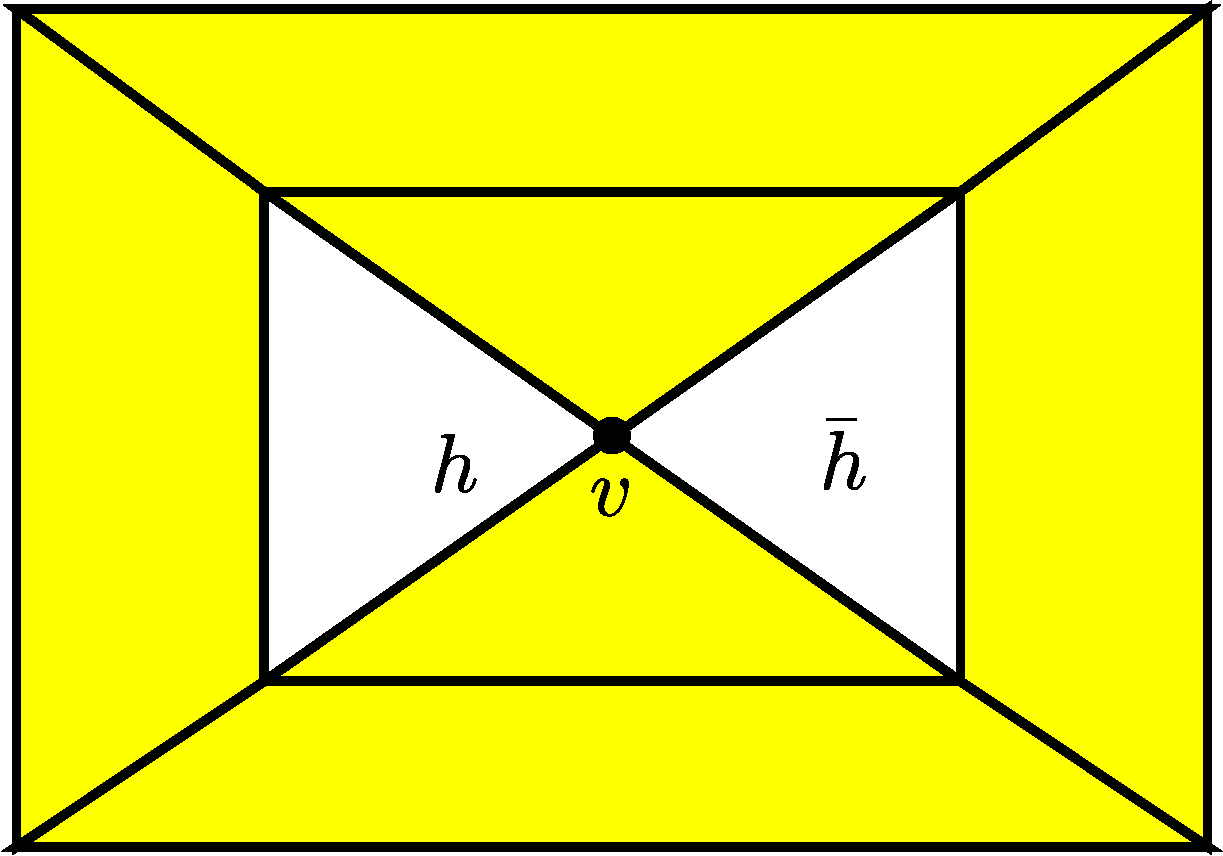
\includegraphics[scale=0.3]{Joint_hole_complex_input-crop}
      \quad
      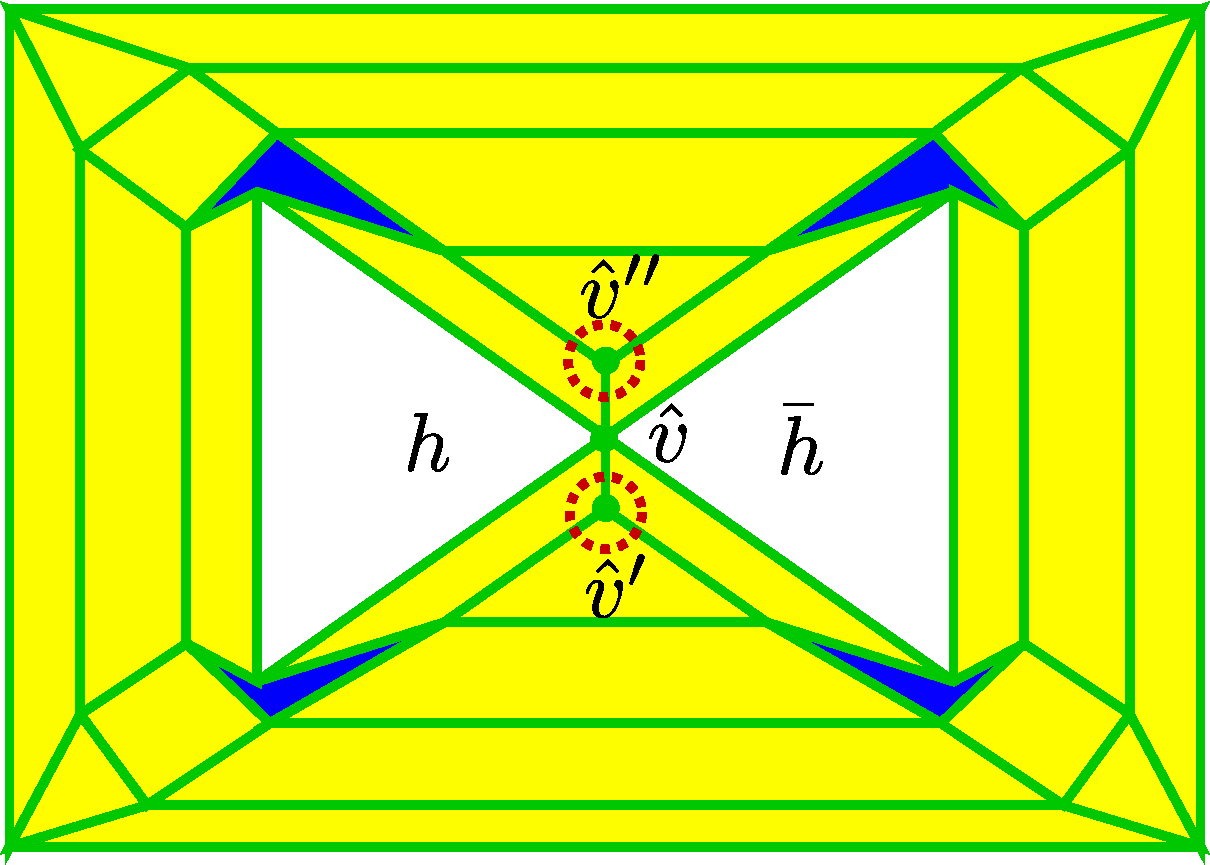
\includegraphics[scale=0.3]{Joint_hole_complex_output-crop}
      \caption{Two holes touching at a vertex (left), and the result of applying Euler transformation (right).
        Vertices with odd degree in the resulting complex are circled.
        The four cells shaded in blue are polygons of Class \ref{2dETcls3} generated by vertices in the input complex (see \cref{ssec:euler2d}).
        These cells could be nonconvex.
      }
      \label{fig:disjholes}
    \end{figure}
    
  }
\end{rem}

We pointed out in the Proof of \cref{lem:hGplanar} that the polygons of Class \ref{2dETcls2} in $\hK$ generated by edges are convex $4$-gons.
Each polygon $\hf \in \hK$  of Class \ref{2dETcls1} is geometrically similar to the polygon $f \in K$ generating it.
Hence if $f$ is convex, so is $\hf$.
But polygons of Class \ref{2dETcls3} generated by vertices are not guaranteed to be convex.
 In fact, when $v \in K$ is a boundary vertex where $K$ has a notch, or an ``incut corner'', $\hf_v \in \hK$ could be nonconvex---see \cref{fig:disjholes} for illustrations.

We finish this section with a result that guarantees $\hK$ remains connected.

\begin{prop}
  \label{prop:hKcnctd2d}
  Assuming the input complex $K$ in $d=2$ is connected, its Euler transformation $\hK$ is also connected.
\end{prop}
\begin{proof}
  We noted in the proof of \cref{lem:hGplanar} that the mitered offset polygons in $\hK$ are pairwise disjoint.
  But we show that when polygons $f,f' \in K$ are connected, so are the corresponding offset polygons $\hf, \hf' \in \hK$.
  By \cref{asmn:Kholesoutside} on the input complex, when polygons $f,f' \in K$ intersect, they do so either in an edge $e$ or in a vertex $v$.
  If $f \cap f' = e$, then by the definition of Euler transformation (\cref{ssec:euler2d}), the corresponding offset polygons $\hf,\hf' \in \hK$ are connected by the pair of new edges defining $\hf_e$, the $4$-gon of Class \ref{2dETcls2} generated by edge $e$.
  If $f \cap f' = v$ and $v$ is not an articulation vertex, then the corresponding offset polygons $\hf,\hf' \in \hK$ are similarly connected by the Class \ref{2dETcls3} polygon $\hf_v$ generated by $v$, with the corresponding copies $\hv, \hv'$ of $v$ in $\hf,\hf'$, respectively, being vertices of $\hf_v$.
  If $f \cap f' = v$ that is an articulation vertex, then $\hv=v$ is the identical copy of this vertex in $\hK$.
  There will be two Class \ref{2dETcls3} polygons $\hf_v, \hf_v'$ generated by $v$ in the two biconnected components joined at $v$, with $\hf_v \cap \hf_v' = \hv$.
  Further, $\hf_v$ is connected to $\hf$ and $\hf_v'$ to $\hf'$, ensuring that $\hf$ and $\hf'$ are connected.
  It follows that $\hK$ is connected, since we assume the input complex $K$ is connected.
\end{proof}
\subsection{Geometric Realization in $d=3$} \label{ssec:rlzn3d}

  \vspace*{-0.3in}
  \addtocounter{thm}{-1}
  
We restrict discussion of geometric realization in 3D to the case where $3$-cells in $\hK$ are homeomorphic to a $3$-ball and edges are straight lines, but $2$-cells can be non-planar.
For the sake of completeness, we relist the assumptions on the input complex $K$ in $d=3$ here.
\begin{asmn}
  \label{asmn:3dKCHCO}
  In dimension $d=3$, the input complex $K$, holes $\CH$, and the outside cell $\CO$ are assumed to satisfy the conditions specified in \cref{asmn:Kholesoutside}.
  In addition, we assume that the degree of each vertex $v$ in each $3$-cell $t \in K$ containing $v$ is $3$.
  In other words, each vertex $v \in t$ is connected to exactly three other vertices $v' \in t$.
\end{asmn}

It follows from \cref{asmn:3dKCHCO} that a vertex $v$ in a $3$-cell $t \in K$ is shared by exactly three polygons that are facets of $t$.
Tetrahedral,  cubical, and rectangular cuboid meshes are examples of polyhedral complexes satisfying the degree $3$ condition.

We first present the main result on same even degree of vertices in the Euler transformation.

\begin{thm} \label{thm:deg6ET3d}
  Every vertex in $\hK$, the Euler transformation of the $3$-complex $K$, has degree $6$ in the $1$-skeleton of $\hK$.
\end{thm}
\begin{proof}
  Consider a vertex $\hv \in \hK$ that is part of the $3$-cell $\htt$, added as a Class \ref{3dETcls1} mitered offset copy of the $3$-cell $t \in K$ (see \cref{ssec:euler3d}).
  Let $v$ be the corresponding vertex in $t$.
  Since \cref{asmn:3dKCHCO} holds for $K$, vertex $v$ has degree $3$ in $t$ and is part of three polygons $\{f_i\}_{i=1}^3$ that are facets of $t$.
  As $\htt$ is a mitered offset of $t$, vertex $\hv$ has the identical degree of $3$ in $\htt$.
  Further, each $f_i$ generates a Class \ref{3dETcls2} $3$-cell $\htt_{f_i}$ in $\hK$ (see \cref{ssec:euler3d}) for $i=1,2,3$.
  Vertex $\hv$ is connected to one \emph{new} edge of the form  $\{\hv,\hv'_i\}$ in $\htt_{f_i}$ (disjoint from $\htt$) for $i=1,2,3$.
  These three edges bring the total degree of $\hv$ in the $1$-skeleton of $\hK$ to $6$.
\end{proof}

\begin{prop}
	\label{prop:transcomplex}
	Homology of $\hK$ do not change.
\end{prop}
Since $\hK$ and $K$ always have same underlying space.
\begin{rem}
  \label{rem:nonplnr3d}
  {\rm
  	While $3$-cells of each Class has a guaranteed geometric realization in $\R^3$ but some facets for $3$-cells belonging to Classes \ref{3dETcls3} and \ref{3dETcls4} can be non planar.
    %While $3$-cells of Classes \ref{3dETcls1} and \ref{3dETcls2} are guaranteed to have geometric realizations in $\R^3$, the same cannot be guaranteed for $3$-cells belonging to Classes \ref{3dETcls3} and \ref{3dETcls4}.
    In particular, if the cells in $K$ are assumed to be convex, then all Class \ref{3dETcls1} cells are also convex, since they are mitered offsets of the convex cells in $K$.
    In this case, the Class \ref{3dETcls2} cell $\htt_f$ generated by the convex polygon $f$ is also guaranteed to be convex, as each of the $p$ $4$-gon added is planar (see \cref{fig:3dETcls2}).
    
    The problem arises for the two $q$-gons added as part of each Class \ref{3dETcls3} cell---they may not be planar even if all edges $\he_j$ are identical in length.
    Instead of the depiction in \cref{fig:3dETcls3}, we might have the $q$-gon(s) as shown in \cref{fig:3dETcls3nplr}.
    We will find the best fit plane through all the vertices in question, and project the vertices up or down to the plane as needed by extending or shrinking edges as shown in the \cref{fig:3dETcls3nplr}
    %We can find a plane passing through subset of the points in  non-planar $q$-gon and project rest of the vertices of $q$-gon not in that plane by extending the edges as shown in the \cref{fig:3dETcls3nplr}. 
    %We might have to triangulate the $q$-gon for a geometric realization in this case.
    \begin{figure}[htp!]
      \centering
      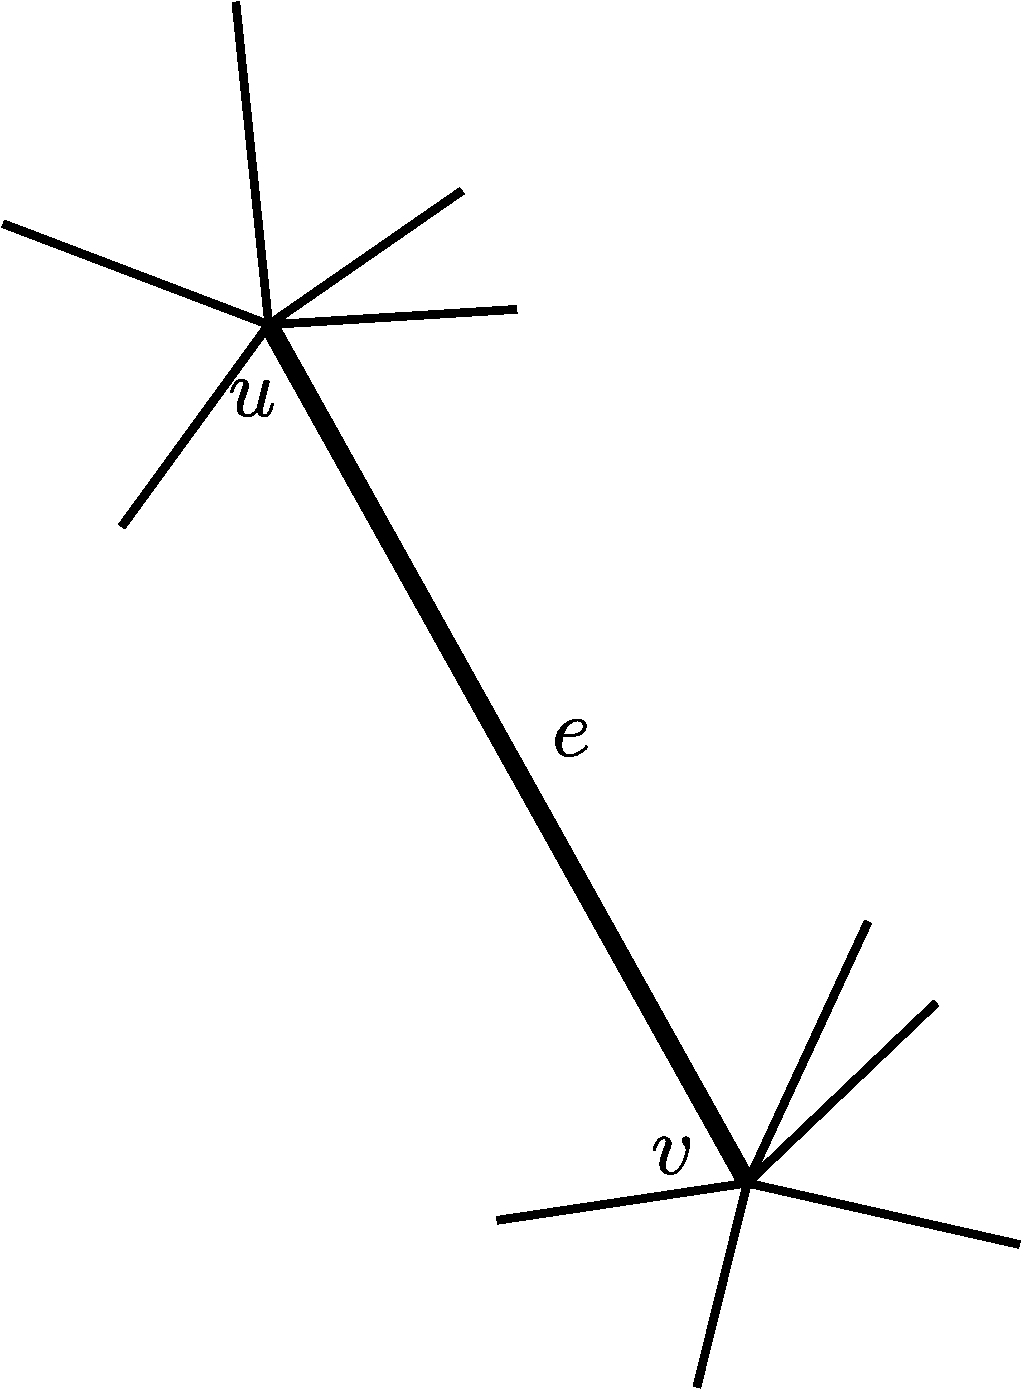
\includegraphics[scale=0.2]{euler_transformation_3d_around_edge_input-crop.pdf}
      \hspace*{0.1in}
      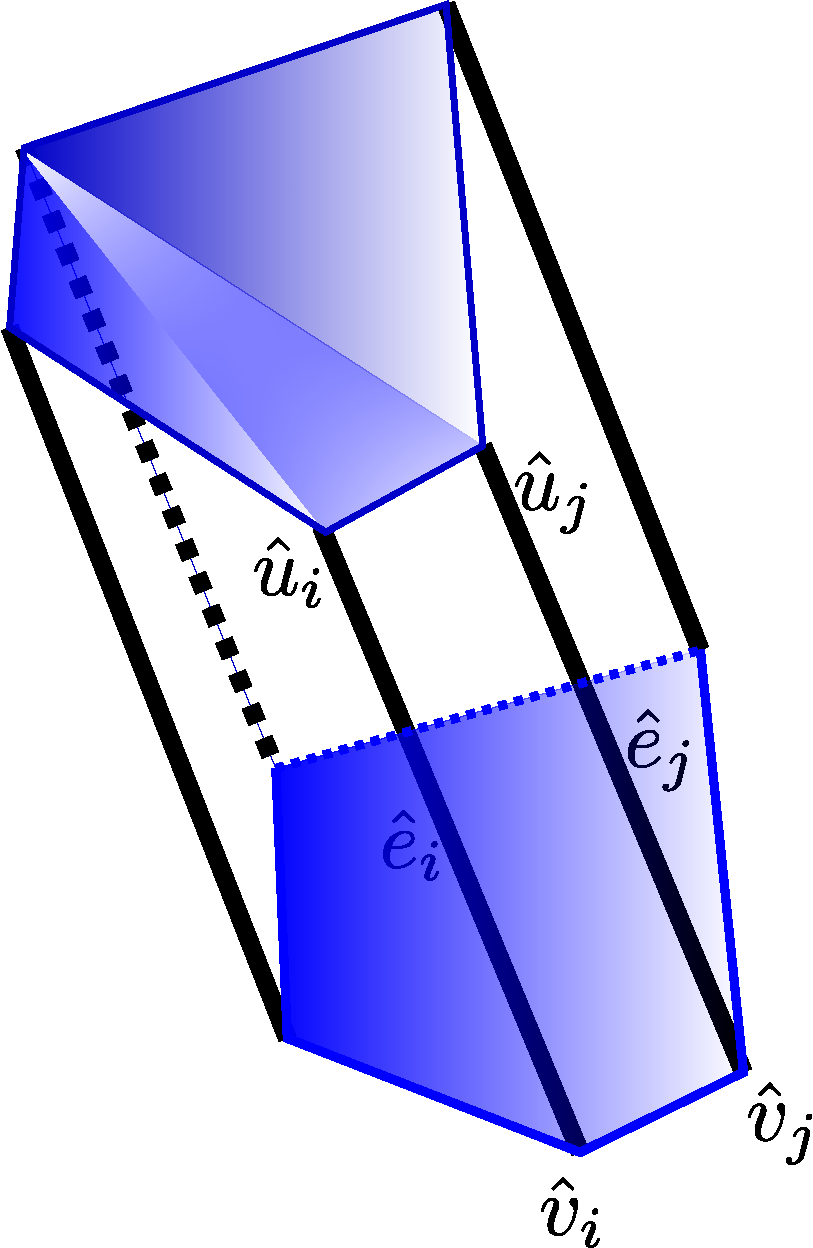
\includegraphics[scale=0.2]{euler_transformation_3d_around_edge_output_nonplanar-crop.pdf}
      \hspace*{0.1in}
      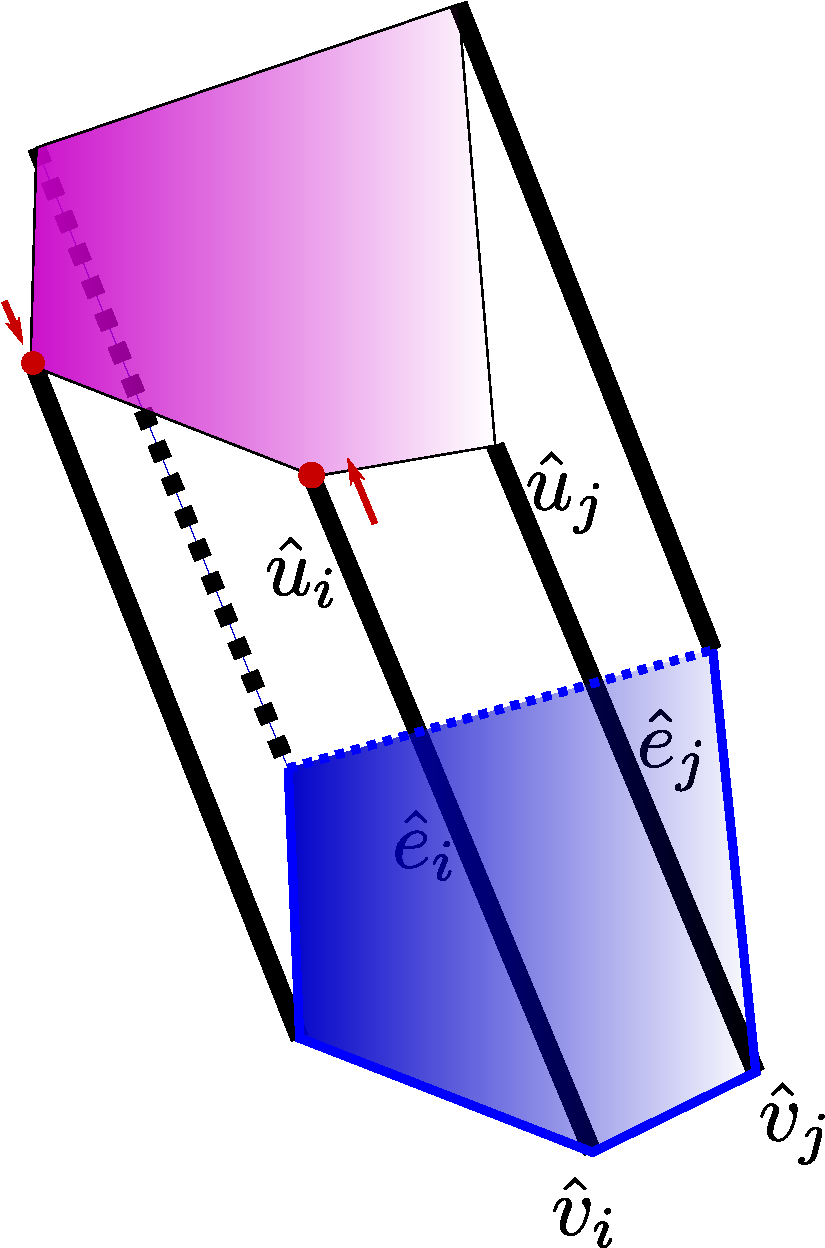
\includegraphics[scale=0.2]{euler_transformation_3d_around_edge_output_nonplanar_to_planar-crop.pdf}
      \caption{
        Input edge $e \in K$ shared by $5$ cells (left), just as shown shown in \cref{fig:3dETcls3}.
        But here, the pentagon on top in the Class \ref{3dETcls3} $3$-cell $\htt_e$ (middle) is not planar as originally set.
        This pentagon is replaced by the best fit plane (right, in pink) where one vertex is pushed up and another one down (red dots) while other vertices remain at their original positions. 
      }
      \label{fig:3dETcls3nplr}
    \end{figure}
    
    If the input complex is highly regular, e.g., a cubical complex with nearly identical cell sizes, it might be possible to choose the mitered offsets of each cell such that these polygons are indeed planar.
    But if such choices do not exist, we can project these points to a plane as discussed. 
    %But if such choices do not exist, we could consider triangulating each $q$-gon in such a way that the degree of each vertex $\hv_i$ stays even.
    %To this end, we could consider all candidate polygons that are facets of the Class \ref{3dETcls4} cell generated by vertex $v$, and add edges in their triangulations in such a fashion that they form cycles, thus ensuring we increase the degree of each vertex $\hv_i$ by even numbers.
    %But it is an open problem if we can always construct such triangulations.

    At the same time, for our motivating applications including infill lattice printing in additive manufacturing and coverage problems in robotics, we are concerned only with the $1$-skeleton of $\hK$.
    And the $1$-skeleton on $\hK$ is completely determined by the $3$-cells of Classes \ref{3dETcls1} and \ref{3dETcls2}.
    Hence we could just \emph{not} include $3$-cells of Classes \ref{3dETcls3} and \ref{3dETcls4} in $\hK$.
    Naturally, the underlying space $|\hK|$ will not be homeomorphic to $|K|$ because of the missing $3$-cells (we can show that $|K|/|\hK|$ is a single enclosed void).
    But the $1$-skeletons cover the same domain.
  }
\end{rem}

We now present bounds on the numbers of each class of cells in $\hK$ as multiples of corresponding numbers in $K$.
The counts would be lower if we do not include $3$-cells of Classes \ref{3dETcls3} and \ref{3dETcls4}.

\begin{lem}
  \label{lem:cntshThVhEhf3d}
  Let $V,E,F,T$ denote the sets of vertices, edges, polygons (faces), and $3$-cells in $K$, and let $\hV, \hE, \hF, \hT$ denote the corresponding sets in $\hK$.
  Let $\nu$ denote the maximum number of vertices in any $3$-cell in $K$, and let $\pi$ denote the maximum number of edges in any polygon (face) in $K$.
  The following bounds hold for the cardinalities of the sets of cells in $\hK$.
  \begin{align}
    |\hT| &   =  |T| + |F| + |E| + |V| \label{eq:3dhTsz} \\
    |\hV| & \leq \nu |T|  \label{eq:3dhVbd} \\
    |\hE| & \leq 3 \nu |T| \label{eq:3dhEbd} \\
    |\hF| & \leq (\pi+2)|F| + 2 |E| \label{eq:3dhFbd}
  \end{align}
\end{lem}
%
\begin{proof}
  \cref{eq:3dhTsz} follows from the definition of Euler transformation in $d=3$ in \cref{ssec:euler3d}, where we get a unique $3$-cell in $\hK$ corresponding to each $3$-cell (Class \ref{3dETcls1}), face or polygon (Class \ref{3dETcls2}), edge (Class \ref{3dETcls3}), and vertex (Class \ref{3dETcls4}) in $K$.
  The count will be equal to $|T| + |F|$ if we do not include $3$-cells of Classes \ref{3dETcls3} and \ref{3dETcls4}.

  Any two $3$-cells of Class \ref{3dETcls1} (mitered offsets) in $\hK$ are disjoint, and all vertices in $\hK$ belong to one of these $3$-cells.
  Hence the total number of vertices in $\hK$ is the sum of the number of vertices in each $\htt \in \hV$.
  The bound in \cref{eq:3dhVbd} results from the fact that each $3$-cell $t \in T$ generates a unique mitered offset $3$-cell $\htt \in \hT$, and the maximum number of vertices in any $t$ is $\nu$.

  \cref{thm:deg6ET3d} specifies that the degree of each vertex $\hv \in \hV$ is $6$.
  Hence we get that $2|\hE| = 6|\hV|$, the sum of all degrees in $\hK$.
  Combining this result with the bound in \cref{eq:3dhVbd} gives the bound in \cref{eq:3dhEbd} (assuming we add all Class \ref{3dETcls3} cells).

  Every facet or polygon $f \in F$ with $p$ edges generates a Class \ref{3dETcls2} $3$-cell with $p+2$ polygons as facets.
  Note that this set includes the two copies of $f$ that are facets of mitered offset $3$-cells in $K$ which share $f$.
  We get two \emph{new} polygons from the Class \ref{3dETcls3} $3$-cells generated by each edge $e \in E$.
  The bound in \cref{eq:3dhFbd} now follows since the number of edges of any $f \in F$ is $\pi$.
\end{proof}

We point out that the bounds in \cref{eq:3dhVbd,eq:3dhEbd,eq:3dhFbd} are tight when $K$ is a cell complex with same type of cells.
For instance, if $K$ is a tetrahedral complex, these bounds are tight with $\nu=4, \pi=3$.
If $K$ is a cubical complex, we get tight bounds with $\nu=8, \pi=4$.

\medskip
\noindent We now show that $\hK$ remains connected even if we do not add $3$-cells of Classes \ref{3dETcls3} and \ref{3dETcls4}.

\begin{prop}
  \label{prop:hKcnctd3d}
  Assuming the input complex $K$ is connected in $d=3$, its Euler transformation $\hK$ is also connected even without including Classes $3$ and $4$.
\end{prop}
\begin{proof}
  Observe that any pair of mitered offset $3$-cells $\hK$ (Class \ref{3dETcls1} cells specified in \cref{ssec:euler3d}) are disjoint by definition.
  But we show that if $K$ is connected, then so is $\hK$ even if we do not include $3$-cells of Classes \ref{3dETcls3} and \ref{3dETcls4}.
  By \cref{asmn:3dKCHCO}, when $3$-cells $t,t' \in K$ intersect in a polygon $t \cap t' = f$, then by the definition of Euler transformation (\cref{ssec:euler3d}), the corresponding offset polygons $\htt,\htt' \in \hK$ are connected by a new Class \ref{3dETcls2} $3$-cell $\htt_{f}$ generated by the polygon $f$.
  Also, by \cref{asmn:3dKCHCO}, for any two $3$-cells $t,t'$ in a biconnected component of $K$ with $t \cap t' = \emptyset$, there exists a finite sequence of $3$-cells $t_1=t, t_2,\dots,t_{r-1},t_r=t'$ such that $t_i \cap t_{i+1} = f_i$, a polygon, for $i=1,\dots,r-1$.
  Following the previous observation, each pair $\htt_i, \htt_{i+1}$ is connected in $\hK$ by a Class \ref{3dETcls2} $3$-cell $\htt_{f_i}$.
  Hence $\htt,\htt'$ are connected in the same biconnected component in $\hK$.
  Finally, articulation vertices are preserved by the Euler transformation, ensuring that biconnected components of $K$ remain connected in $\hK$.
  Hence it follows that $\hK$ is connected as well, since we assume the input complex $K$ is connected.
\end{proof}

We end this section with an additional nice property of the Euler transformed complex $\hK$: every edge is shared by exactly four polygons, i.e., faces.
As a result, the $2$-complex resulting from the intersection of $\hK$ with a plane in 3D that intersects only the edges but not any vertices in $\hK$ is guaranteed to be Euler.
This result could have implications in 3D printing where one may consider slicing the Euler transformed $3$-complex so as to print 2D layers.


\begin{lem}\label{lem:edgcnct4facs}
  Each edge in $\hK$ is connected to $4$ faces in $\hK$
\end{lem}
\begin{proof}
  We consider two cases for an edge $\he$ in $\hK$: $\he$ is part of some Class \ref{3dETcls1} $3$-cell $\htt$ and $\he$ is not part of any $3$-cell. %(see  \cref{ssec:euler3d} for details ).
  The two cases are illustrated on a cubical $3$-complex in \cref{fig:3dETedgefacerelation}.

  In the first case, $\he$ is the mitered offset of edge $e$ in $3$-cell $t \in K$.
  Let $e$ be shared by polygons $f',f''$ that are faces of $t$.
  Then $\he$ in $\htt$, the mitered offset of $t$, is shared by faces $\hf',\hf''$ of $\htt$, the mitered offset polygons of $f'$ and $f''$, respectively.
  Edge $\he$ is also shared by one polygon each from the two Class \ref{3dETcls2} $3$-cells $\htt_{f'}$ and $\htt_{f''}$, generated by $f'$ and $f''$, respectively.
  These two polygons are also faces of a Class \ref{3dETcls3} $3$-cell $\htt_{e}$ generated by $e$.
  Hence $\he$ is shared by exactly four polygons in $\hK$.

  %Each edge $\he$ is contained in $1$ class-$1$, $2$ class-$2$ and $1$ class-$3$ 3-cells. $\he$ is contained in $2$ faces $\hf, \hf'$ in $\htt$ (class - $1$). $\hf$ is contained in $1$ class-$2$ $3$-cell $t_f$ since every face in $\htt$ is also contained in some class-$2$ $3$-cell. Similarly $\hf'$ is contained in some class-$2$ $3$-cell $t_{f'}$. $t_f, t_{f'}$ contributes $2$ faces $\hf'', \hf'''$ that contains $\he$ since any $2$ same class $3$-cells are face disjoint. $\hf'', \hf'''$ are also contained in $1$ class-$3$ $3$-cell $t_e$ of $\hK$. Hence $\he$ is contained in $4$ faces.

  In the second case, let edge $\he = (\hv, \hv')$ be not contained in any Class \ref{3dETcls1} $3$-cell.
  By construction (see \cref{ssec:euler3d}), edge $\he$ is contained in one Class \ref{3dETcls2} and two Class \ref{3dETcls3} $3$-cells, and also one Class \ref{3dETcls4} $3$-cell separating these two Class \ref{3dETcls3} $3$-cells.
  Observe that no two $3$-cells of the same class in $\hK$ can share a polygon as a face.
  Let edges $e',e''$ meet at vertex $v$ in polygon $f$ in the input $3$-cell $t \in K$.
  Let the corresponding cells in the mitered offset $\htt \in \hK$ be $\he', \he''$ meeting at vertex $\hv$ in polygon $\hf$.
  Then edge $\he$ is contained in two $4$-gons that are faces of the Class \ref{3dETcls2} $3$-cell $\htt_{f}$.
  It is also contained in one polygon each from two Class \ref{3dETcls3} $3$-cells $\htt_{e'}$ and $\htt_{e''}$.
  Note that the last two polygons are also faces of the Class \ref{3dETcls4} $3$-cell $\htt_{v}$ generated by vertex $v$.
  Overall, $\he$ is shared by exactly four polygons in $\hK$.
  Note that We could, equivalently, describe the four polygons with respect to $\htt' \in \hK$, where the polygon $f$ is shared by $3$-cells $t, t' \in K$.
\end{proof}
\begin{figure}[htp!]
  \centering
  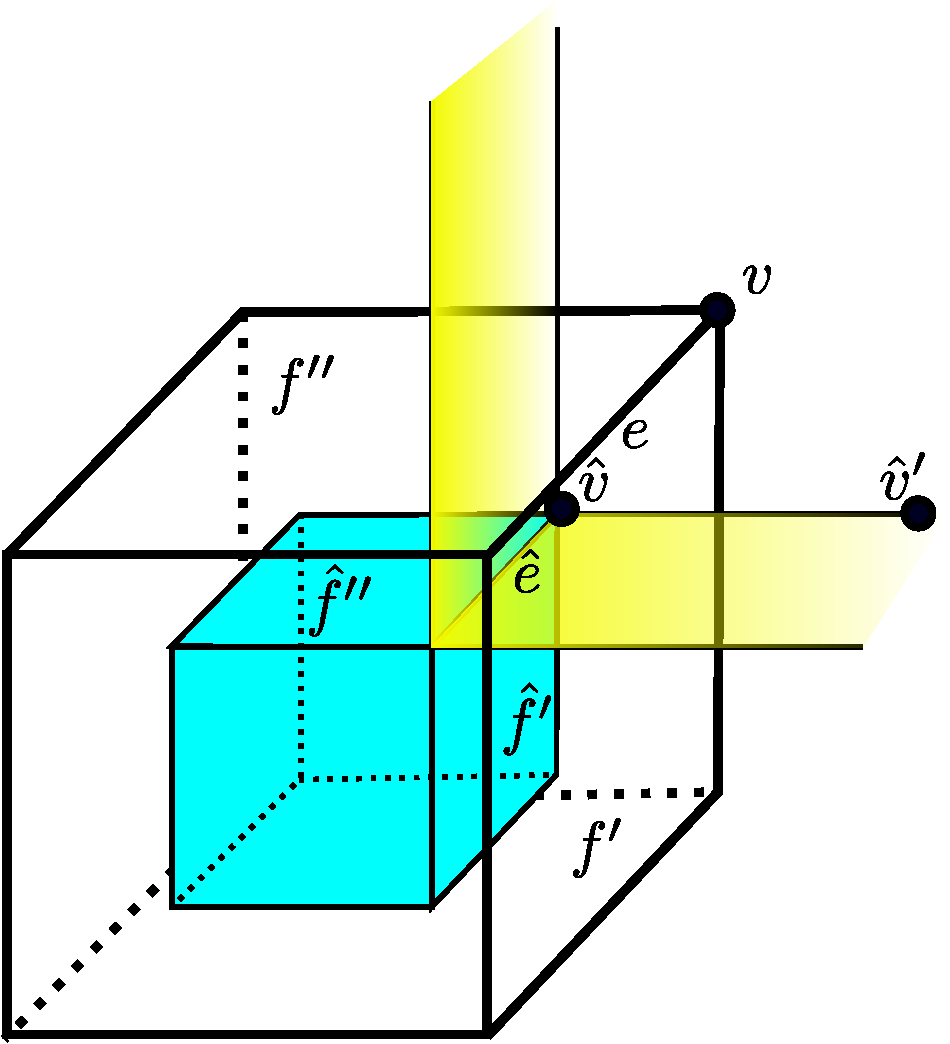
\includegraphics[scale=0.4]{edge_face_relation_fig_0_crop}
  \quad
  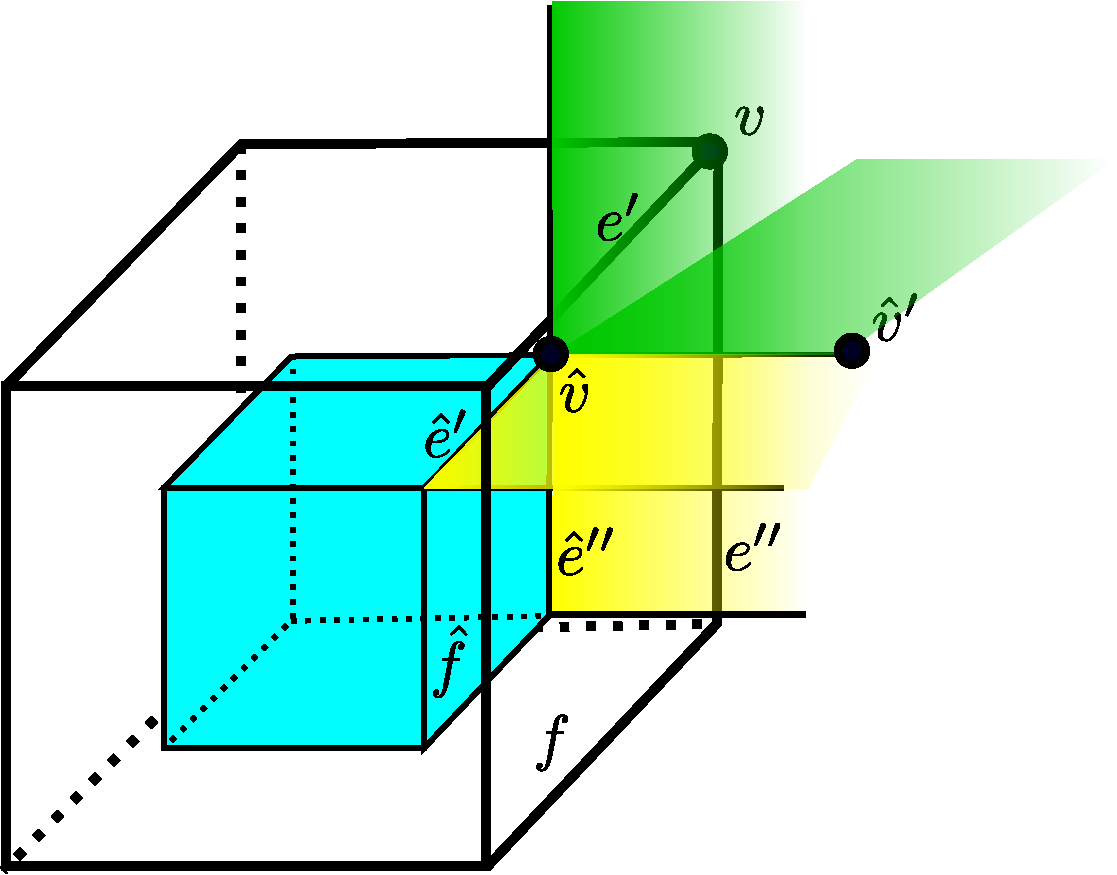
\includegraphics[scale=0.4]{edge_face_relation_fig_1_crop}
  \caption{\label{fig:3dETedgefacerelation}
    Illustration of two cases for edge $\he$ in \cref{lem:edgcnct4facs} on a cubical complex.
    In the first case (left), the $3$-cell $t$ is the cube is shown in white, and its corresponding Class \ref{3dETcls1} $3$-cell $\htt \in \hK$ is shown in blue.
    In the right figure showing the second case, the two $4$-gons of the Class \ref{3dETcls2} $3$-cell $\htt_{f}$ are shown in yellow, and the polygons from two Class \ref{3dETcls3} $3$-cells are shown in green.\\
    }
\end{figure}
\begin{prop} \label{rem:2DsliceEuler}
  Let $\cP$ be a plane in $\R^3$ such that $\sigma \not\in \cP$ for every simplex $\sigma \in \hK$, the Euler transformed $3$-complex.
  Then the $1$-skeleton of the $2$-complex that is $\cP \cap \hK$ is Euler.
\end{prop}
\begin{proof}
  Since the plane $\cP$ does not contain any simplex of $\hK$, vertices in the resulting $2$-complex $\cP \cap \hK$ are created by $\cP$ intersecting edges in $\hK$.
  \cref{lem:edgcnct4facs} says each edge $e \in \hK$ is a face of exactly four polygons.
  Hence the vertex generated by $\cP \cap e$ will have degree $4$, with four edges generated by $\cP$ intersecting each of the four polygons that share $e$.
\end{proof}

Finally, we consider what happens if the restriction that each vertex has degree $3$ in each $3$-cell that contains the vertex in the input complex $K$ is not satisfied.
\begin{rem}\label{rem:3dETdeg4vtx}
  {\rm 
    As a example where the assumption of vertices with degree $3$ in each cell does not hold, consider a $3$-cell $t$ that is a pyramid with a trapezium at the base, as shown in  \cref{fig:mothde3ver}.
    Let vertex $v$ be the one on top with degree $4$ in the $1$-skeleton of $t$.
    Then the mitered offset $\ttt$ created after even an infinitesimal shrinkage will replace $v$ in $K$ with a face $\tf$ in the resulting complex $\tK$, instead of a corresponding single vertex $\hv$ \cite{AuWa2013,AuWa2016}.
    But since $v$ has degree $4$ in $t$, \cref{thm:deg6ET3d} is not valid, and we could get vertices with odd degrees.
    For instance, $\tv$ in \cref{fig:mothde3ver} has degree $5$.
    Nevertheless, every vertex in the $1$-skeleton of $\ttt$ will now have degree $3$.
    More generally, every vertex in the $1$-skeleton of $\tK$ obtained in this fashion has degree $3$, and it satisfies all requirements of \cref{asmn:Kholesoutside} of an input complex.
    If we apply Euler transformation \emph{again} on $\tK$, we are guaranteed to obtain a $3$-complex $\hK$ that satisfies all previous results presented in this Section.
    This situation is similar to the one in 2D described in \cref{rem:adjbdyedges}.
}	
\end{rem}
\begin{figure}[htp!]
  \centering
  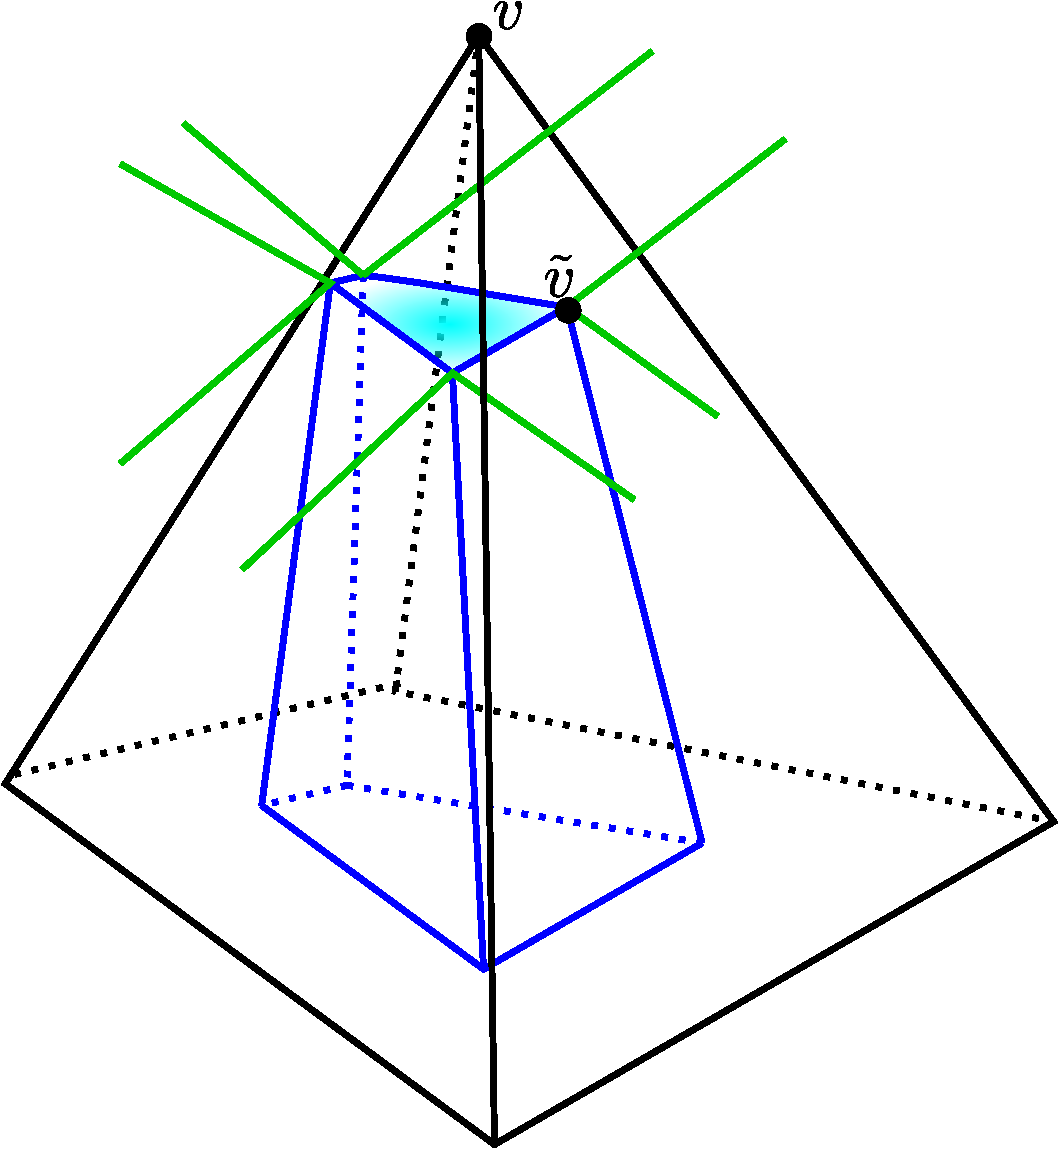
\includegraphics[scale=0.45]{more_than_degree_3_vertex_fig_0_crop}
  %\includegraphics[scale=0.5]{MyMoreThanDeg3VertexFig-crop}
  \caption{\label{fig:mothde3ver}
    A pyramid ($3$-cell) $t$ (black edges) in $K$, where vertex $v$ has degree $4$.
    The mitered offset of $t$ with infinite shrinkage $\ttt$ (blue edges) has vertices with degree $5$ in $\ttt$, e.g., $\tv$.
    But any vertex $\tv$ in $\ttt$ has degree $3$ in its $1$-skeleton, and hence satisfies the input assumption for applying Euler transformation.}
\end{figure}
\section{Measures of Geometric Quality} \label{sec:geomqual}

We inspect measures of geometric quality of the cells in the Euler transformation, and study how they compare with corresponding measures for the input complex.
We show that the user can choose a small set of parameters for each top-dimensional cell ($2$- or $3$-cells) in order to control these measures of quality.

Several measures of element quality are used in various domains ranging from numerical analysis, to finite element methods, to computer graphics \cite{ChDeSh2012,GiRaBa2012,LiEbZh2009,Si2010}.
We concentrate mostly on an \emph{aspect ratio} as defined below, but also present results on minimum edge lengths and angles in the 2D case.
\begin{defn}
  \label{def:asptrto}
  For a given $d$-cell $g$, let $\diam(g)$ denote its \emph{diameter}, i.e., the largest Euclidean distance between any two points in $g$.
  Also, let $\rho(g)$ denote its \emph{inradius}, i.e., the radius of the largest $d$-ball inscribed in $g$.
  The \emph{aspect ratio} of the cell is defined as
  \begin{equation}
    \label{eq:asptrto}
    \g(g) = \frac{\diam(g)}{\rho(g)} \,.
  \end{equation}
\end{defn}
%Note that the diameter is twice the circumradius, and hence $g$ is twice the ratio of circumradius over inradius, another commonly used aspect ratio.

\subsection{Geometric quality in $d=2$} \label{ssec:qual2d}

We consider the three classes of polygons generated in the Euler transformation $\hK$ corresponding to polygons, edges, and vertices in $K$ (\cref{ssec:euler2d}).
Since a Class \ref{2dETcls1} polygon $\hf$ is a mitered offset of the corresponding polygon $f \in K$, the user can choose parameters that control how $\hf$ is scaled with respect to $f$.
We consider two parameters ($\gl, \mu$) that control how edge lengths scale, and the offset parameter $b$, which is the perpendicular distance that each edge is pushed in when offsetting.
We choose $\gl$ and $\mu$ based on quality criteria and such that \cref{eq:edmamiratio} is satisfied.
  Based on $\gl$ and $\mu$ chosen, we get from \cref{eq:edofbound} a range of values for $b$.
  And value for $b$ could be chosen from this feasible range.   
We specify ranges for values of these parameters in terms of measures associated with $f$, i.e., input data, which guarantee there are no topological or combinatorial changes in the polygon when offsetting.
We specify these ranges for \emph{each} polygon.
The user could choose a uniform set of values over the entire complex, but the individual ranges afford more flexible choices.

Let $0 < \gl < \mu < 1$ be chosen such that $\gl |e| \leq |\he| \leq \mu |e|$ holds for each edge $e \, \subset f \in K$.
These parameters are specific to $f$, but we do not use $\gl_f,\mu_f$ and so on in order to keep notation simpler.
We illustrate the constructions in \cref{fig:2dETcls1edgeconstr}.
Intuitively, the user may want to choose $\gl$ not too large and $\mu$ not too small in order to get good quality measures (bounded aspect ratio, minimum edge length, or maximum interior angle).
Let $b$ denote the offset distance for edge $e=\{u,v\}$, and let $r_u,r_v$ the corresponding distances for $u,v$.
By properties of mitered offset, choosing an edge length ratio (in $(\gl,\mu)$) and $b$ determines $r_u$ and $r_v$.
We denote by $p,q$ the projection lengths of $r_u, r_v$, respectively, on edge $e$.
\begin{figure}[htp!]
  \centering
  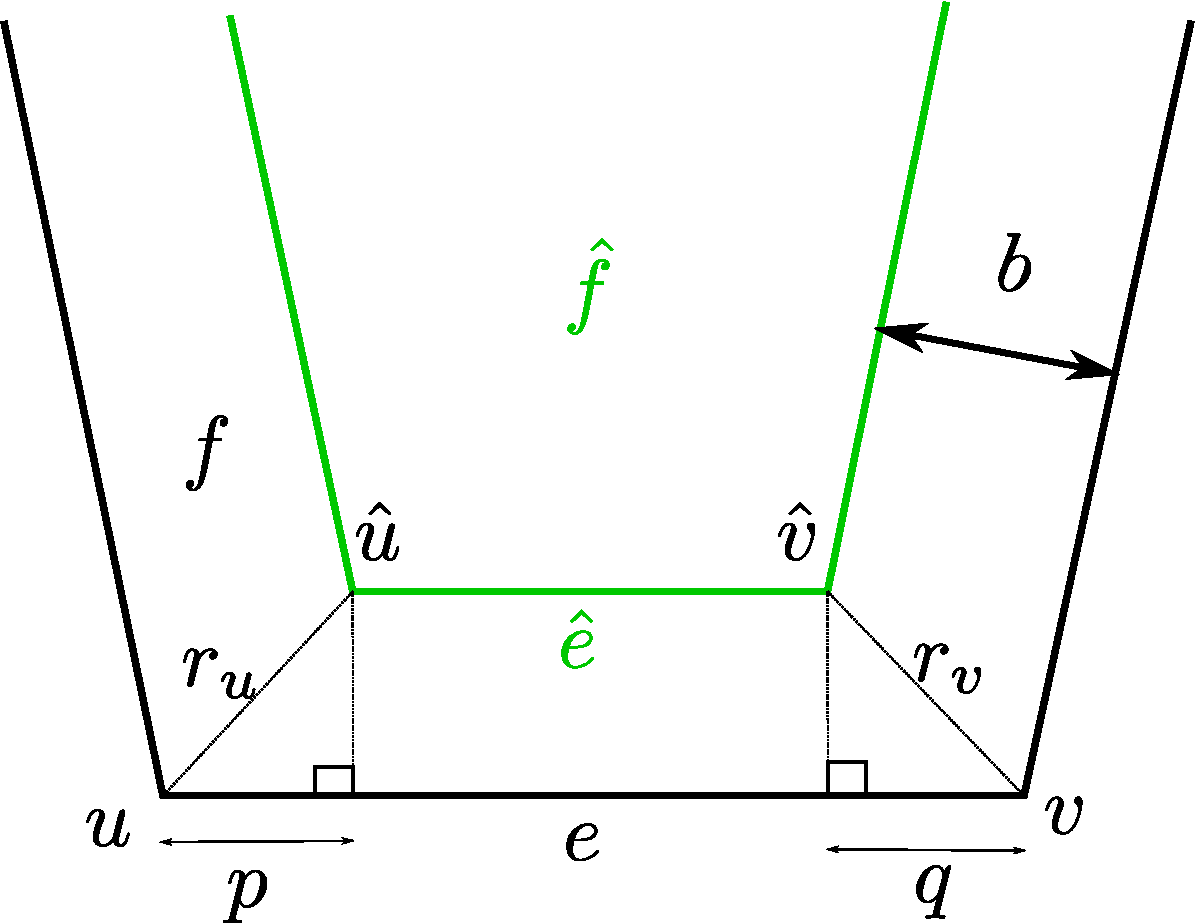
\includegraphics[scale=0.3]{geometry_restriction_etg_edge-crop_edit}
  \caption{Offset polygon $\hf \in \hK$ (in green) and input polygon $f \in K$ (in black), with associated offset parameters.}
  \label{fig:2dETcls1edgeconstr}
\end{figure}

Since $\mu |e|\geq |\he| \geq \gl |e|$ we get $(1 - \mu) |e|\leq p + q \leq (1 -\gl) |e|$.
  To satisfy this range for $p + q$ we further restrict $(1 - \mu)|e|/2 < r_u, r_v < (1 - \gl)|e|/2$.
  Then we get $(1 -\mu) |e|/2 < p, q, b < (1 -\gl) |e|/2$.

Denoting by $|e_{\min}|, |e_{\max}|$ the minimum and maximum edge lengths in $f$, we get the following inequalities.

\begin{align}
  \frac{(1 -\mu)|e_{\max}|}{2} & < b < \frac{(1 -\lambda)|e_{\min}|}{2}\, \mbox{ and } \label{eq:edofbound} \\
  \frac{(1 -\mu)|e_{\max}|}{2} & < r_u, r_v < \frac{(1 -\lambda)|e_{\min}|}{2}, \mbox{ which imply} \label{eq:vrofbound} \\
  \frac{|e_{\max}|}{|e_{\min}|} & ~~ < ~~ \frac{1- \lambda}{ 1- \mu} \, . \label{eq:edmamiratio}
\end{align}

We now specify bounds on quality measures for polygons in each of the three classes.
\subsubsection{Class \ref{2dETcls1} cells} \label{sssec:2dETcls1gq}
Let $f$ be a Class \ref{2dETcls1} polygon, and $b$ the edge offset distance for $\hf$.
Let $D, \hD$ be the diameters and $\rho, \hrho$ the inradii of $f \in K$ and $\hf \in \hK$, respectively.
See \cref{fig:2dETcls1gq} for details. 
\begin{figure}[htp!]
  \centering
  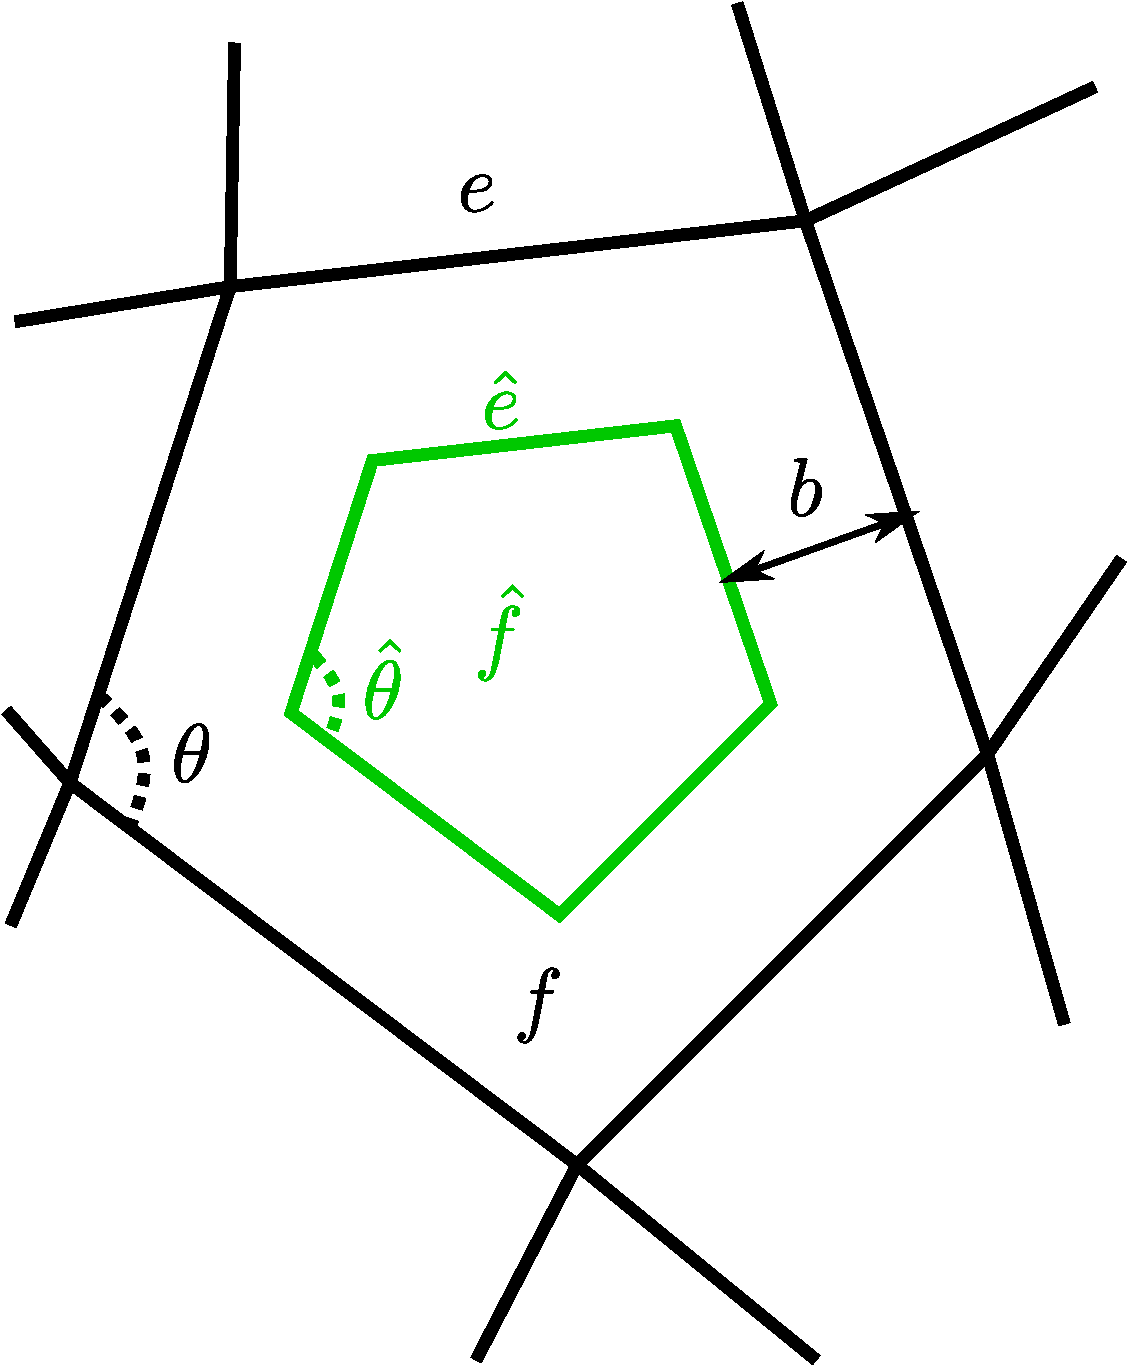
\includegraphics[scale=0.25]{class_1_cell_gq_fig_1-crop}
  \caption{Quality measures for a Class \ref{2dETcls1} polygon $\hf$.}
  \label{fig:2dETcls1gq}
\end{figure}

\begin{description}
\item[Bounded Aspect Ratio]\label{bas:2dETcls1}
We know that $D \geq \hD$ and $\hrho \geq \rho - b$, and hence we get 
\begin{equation} \label{eq:2dETcls1ar}
    2 < \ghf \leq \frac{D}{\rho(1 - \frac{b}{\rho})} =\frac{\g(f)}{(1 - \frac{b}{\rho})}  \,.
\end{equation}
Since offset distance $b$ cannot be more than the inradius $\rho$, we have  $\frac{b}{\rho} < 1$. 
\item[Minimum Edge Length]\label{mel:2dETcls1}
\begin{equation}
    \mbox{Since } |\he| \geq \gl |e| ~\forall e \in K, \mbox{ we get } |\he_{\min}| \geq \gl |e_{\min}| \,.
\end{equation}
\item[Maximum Interior Angle]\label{mia:2dETcls1}
  Since we are using mitered offsets, any interior angle  $\hat{\theta}$ in $\hf$ is same as the corresponding angle $\theta$ in $f$.
  Hence the maximum interior angle in $\hf$ is same as that in $f$.  
\end{description}

\subsubsection{Class \ref{2dETcls2} cells} \label{sssec:2dETcls2gq}
Let $r, r'$ be the offset distances for vertices $\hv, \hv'$ generated by $v \in e \in f, f' \in K$, and let $\he, \he'$ be the corresponding edges in $\hf, \hf'$, respectively.
Let $d$ be a diagonal in the Class \ref{2dETcls2} polygon $\hf_e$.
As in the previous Section, we let $D, \hD$ be the diameters and $\rho, \hrho$ the inradii of $f, \hf_e$, respectively.
We refer to \cref{fig:2dETcls2gq} for details.
\begin{figure}[htp!]
      \centering
      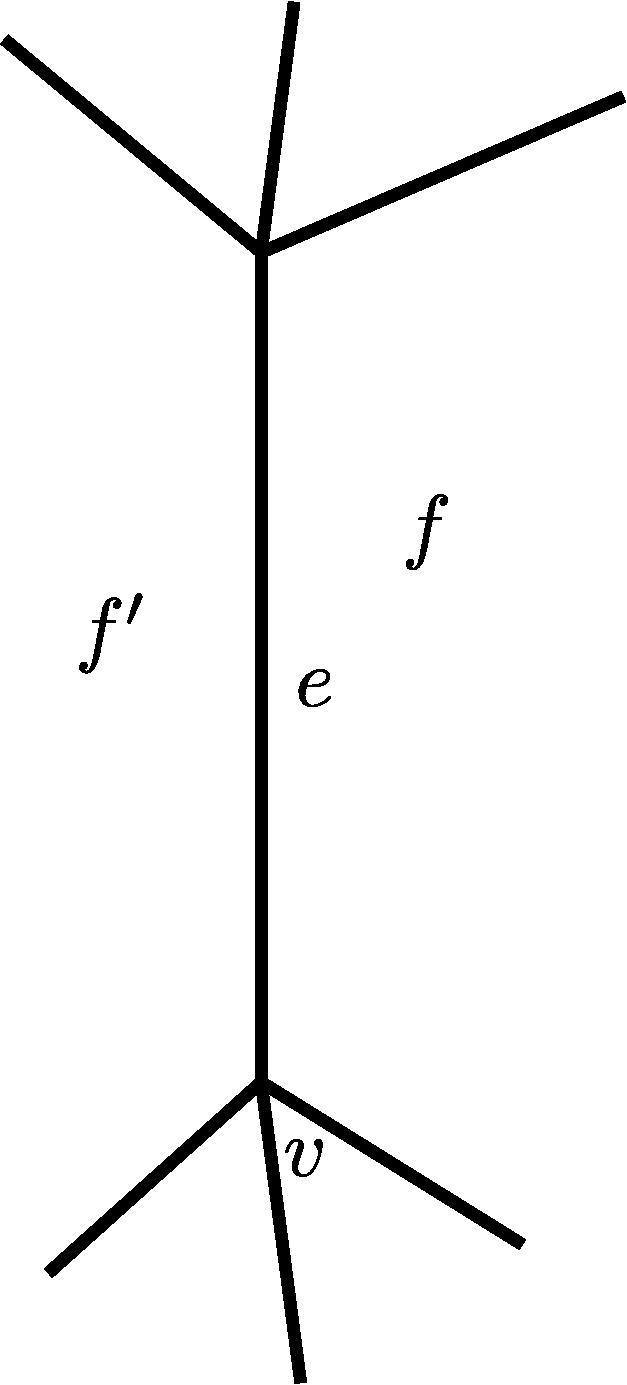
\includegraphics[scale=0.25]{class_2_cell_gq_fig_1-crop}
      \quad\quad
      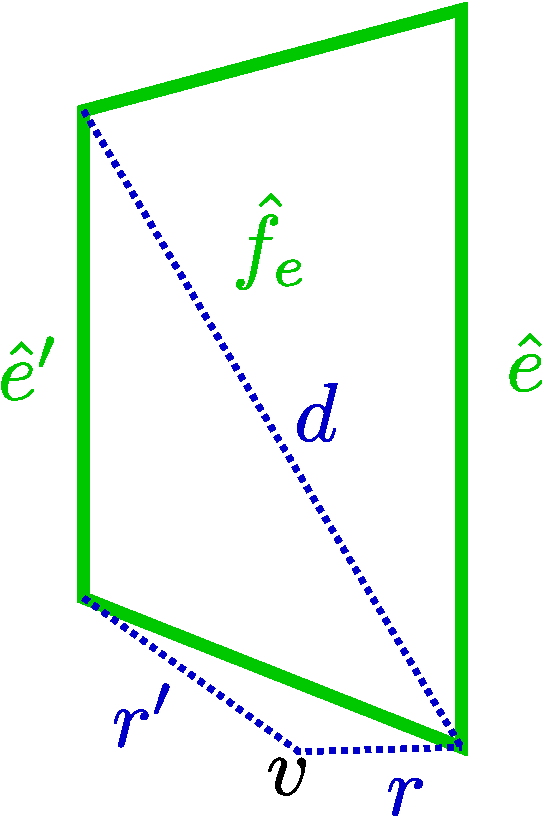
\includegraphics[scale=0.30]{class_2_cell_gq_fig_2-crop}
      \quad\quad
      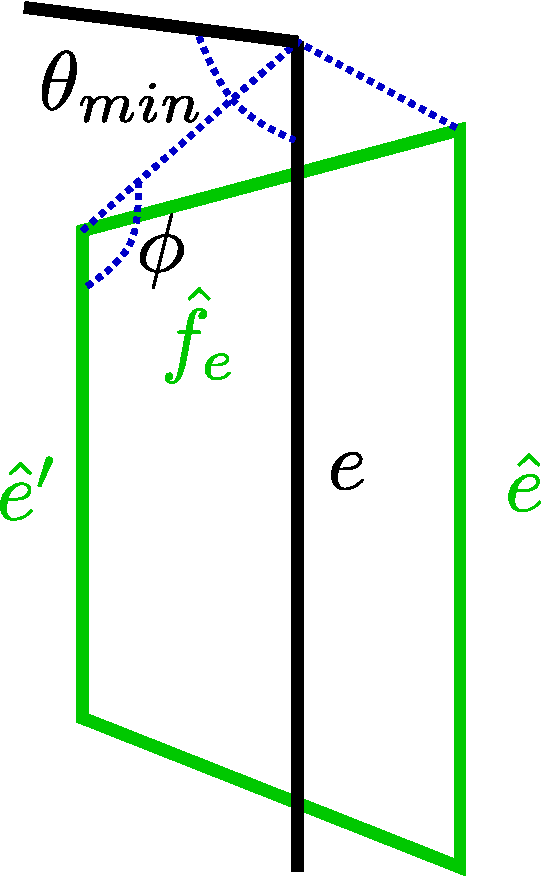
\includegraphics[scale=0.30]{class_2_cell_gq_fig_3-crop}
      \caption{Quality aspects of a Class \ref{2dETcls2} cell $\hf_e$.
      }
      \label{fig:2dETcls2gq}
\end{figure}

\begin{description}
\item[Bounded Aspect Ratio]\label{bas:2dETcls2}
By triangle inequality, we get $|\he'| + r' + r \geq d$. 
Since $|e| \geq |\he'|$, we get
\[ |e| + r' + r \geq d \,. \]
Assume without loss of generality that $\lambda > \lambda'~,~ \mu > \mu'$  and  $|\he'| < |\he|$.
Then by \cref{eq:vrofbound}, we get
\begin{equation}
  ((1 - \lambda') + 1)|e| > d\,.   
\end{equation}
And since diameter of $\hf_e$ is not smaller than the maximum edge length and maximum diagonal length of a trapezium, we have $\hD < ((1 - \lambda') + 1)|e|$.
Using \cref{eq:edofbound}, and since $\mu > \mu' \text{ and } |\he'| < |\he| $ we get 
\begin{equation}\label{eq:bas:2dETcls2edofset}
  b, b' > 0.5(1 - \mu)|\he'| \,.   
\end{equation}
Then area of $\hf_e$ satisfies $\area(\hf_e) \geq (1 - \mu) |\he'|^2$.
As we know that $|\he'| \geq \lambda' |e| $, we get
\begin{equation}
    \area(\hf_e) \geq (1 - \mu) (\lambda')^2 |e|^2 \, .
\end{equation}
We know that the perimeter of $\hf_e$ satisfies $\per(\hf_e) \leq 4|e|$.
Since $\area(\hf_e) \leq \per(\hf_e) \hrho$ as $\hf_e$ is a trapezium \cite{ScAw2000}, we get
\begin{equation}
  \hrho > \frac{(1 - \mu ) (\lambda')^2 |e|}{4} \,.
\end{equation}
Hence
\begin{equation}
  2 < \g(\hf_e) < \frac{4 ((1 - \lambda') + 1)}{(1 - \mu) (\lambda')^2}\, .    
\end{equation}
\item[Minimum Edge Length]\label{mel:2dETcls2}
  Based on our assumption that $|\he'| < |\he|$, we have $\lambda' < \mu$.
  The other two non-parallel edges of $\hf_e$ have lengths at least $b + b'$.
  Hence the minimum edge length of $\hf_e$ is at least $\min \{|\he'|, b+b' \}$, which, by \cref{eq:bas:2dETcls2edofset}, is at least $\min\{ \lambda' |e|, (1 - \mu)\lambda' |e|\} = (1 - \mu)\lambda' |e|$.
  If $e$ is a boundary edge of $f$, the result remains same except $\lambda' = \lambda$ since $e$ is shared between $f$ and $\CH \cup \CO$. 

\item[Maximum Interior Angle]\label{mia:2dETcls2}
  Assume without loss of generality that the minimum interior angle of $f$ is smaller than that of $f'$.
  If $\theta_{\min}$ is the minimum interior angle of f, then the maximum interior angle $\hf_e$ is strictly less than $\phi =\pi - \theta_{\min}/2$ since sum of adjacent interior angles formed by the non-parallel lines with the parallel lines of a trapezium is $\pi$, and in the case of a mitered offset any line segment $u\hu$ shown in \cref{fig:2dETcls1edgeconstr} is an angle bisector for the interior angle at $u$ of the input cell.
  This result is valid in both cases when $e$ is an interior or a boundary edge.
\end{description}

\subsubsection{Class \ref{2dETcls3} cells}  \label{sssec:2dETcls3gq}
Let $r, R'$ be the minimum and maximum offset distances for vertices $\hv, \hv'$, which correspond to vertex $v \in f, f'$, two specific polygons among all that share $v$.
See \cref{fig:2dETcls3gq} for details.
Let $|\tilde{e}_{\min}|, |\tilde{e}_{\max}|$ be the minimum and maximum edge lengths for edges in all $2$-cells sharing vertex $v$, and let the edges belong to $f', f$, respectively.
Let $\alpha, \beta $ are maximum and minimum angles formed by edges of $\hf_v$ on vertex $v$.
Also, let $\lambda, \mu$ and $\lambda', \mu'$ be the user-defined parameters for $f, f'$, respectively.

\begin{figure}[htp!]
      \centering
      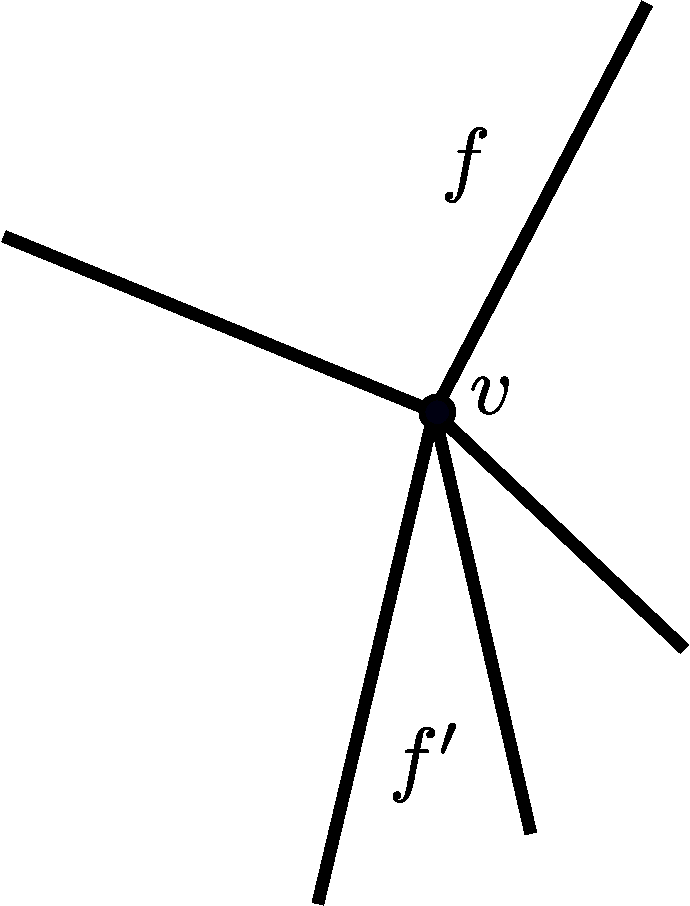
\includegraphics[scale=0.25]{class_3_cell_gq_fig_1-crop}
      \quad
      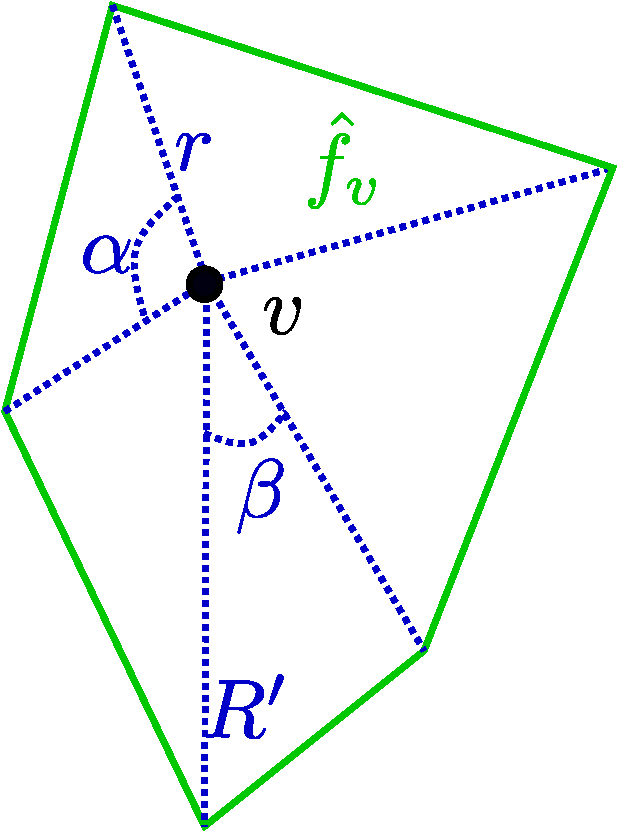
\includegraphics[scale=0.25]{class_3_cell_gq_fig_2-crop}
      \quad
      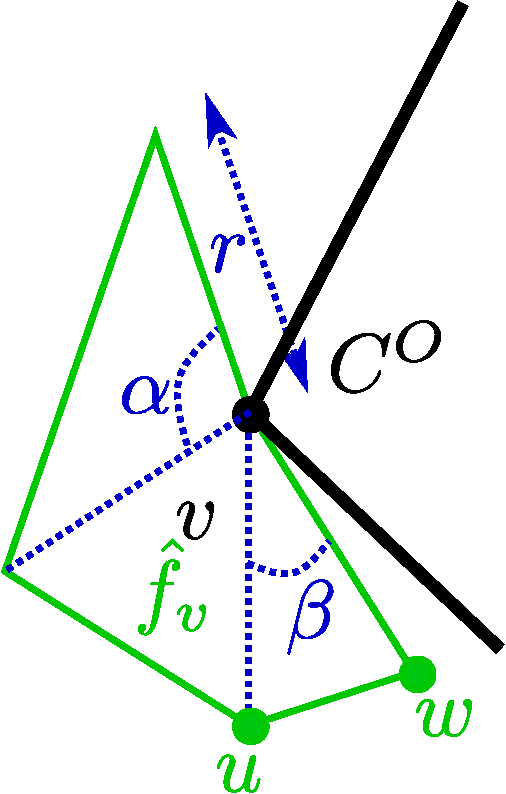
\includegraphics[scale=0.25]{class_3_cell_gq_fig_3-crop}
      \quad
      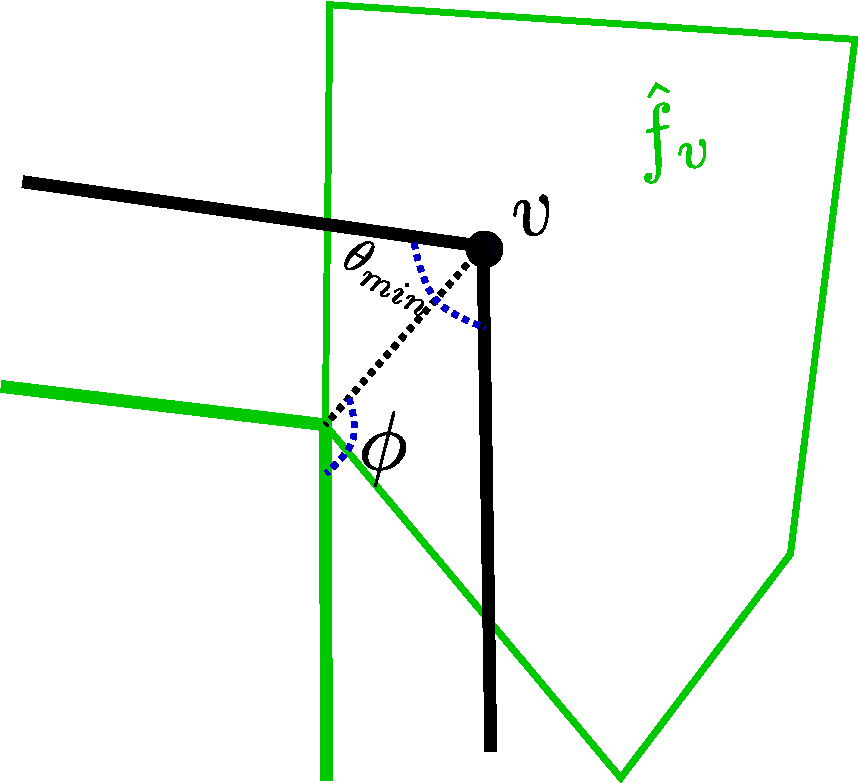
\includegraphics[scale=0.25]{class_3_cell_gq_fig_4-crop}
      \caption{Quality measures for a Class \ref{2dETcls3} cell $\hf_v$.
      }
      \label{fig:2dETcls3gq}
\end{figure}

\begin{description}
\item[Bounded Aspect Ratio]\label{bas:2dETcls3}
  We first consider the case where $v$ is an interior vertex, i.e., it is not on the boundary of $K$.
  Since $\hrho \geq r \cos{\frac{\alpha}{2}}$ and $\hD \leq 2 R'$,  using \cref{eq:vrofbound} gives
  \begin{equation}
    2 < \g(\hf_v) \leq \frac{2R'}{r\cos{\frac{\alpha}{2}}} < C\bigg(\frac{1 - \lambda'}{1 - \mu}\bigg) 
  \end{equation}
  where $C = 2 |\tilde{e}_{\min}| /(|\tilde{e}_{\max}| \cos{\frac{\alpha}{2}})$.
  
  When $v$ is on the boundary, we consider applying the same offset $r$ to every $2$-cell sharing vertex $v$.
  Under this setting, $\Delta uvw$ is an isosceles triangle (third image in \cref{fig:2dETcls3gq}), and hence its inradius is $r \sin(\frac{\beta}{2}) \sqrt{(1- \sin(\frac{\beta}{2}))/(1 + \sin(\frac{\beta}{2}))}$.
  \begin{equation}
    \mbox{Denoting } L = \sin(\frac{\beta}{2}) \sqrt{(1- \sin(\frac{\beta}{2}))/(1 + \sin(\frac{\beta}{2}))},
    \mbox{ we get }~~~~~ \g(\hf_v)  < \bar{C}\bigg(\frac{1 - \lambda'}{1 - \mu}\bigg)~
  \end{equation}
  where, $ \bar{C} = 2|\tilde{e}_{\min}| / (|\tilde{e}_{\max}| L)\,$.

\item[Minimum Edge Length]\label{mel:2dETcls3}
If $v$ is not on the boundary, we get
\begin{equation}
    |\he| \geq 2 r \sin{(\frac{\beta}{2})} > (1 - \mu) |\tilde{e}_{\max}| \sin{(\frac{\beta}{2}}) \,.
\end{equation}
If $v$ is on the boundary, we get
\begin{equation}
    |\he| \geq \min\bigg\{ r, 2r\sin{\frac{\beta}{2}}\bigg\} \,.
\end{equation}
Then we get by \cref{eq:vrofbound} that
\begin{equation}
    |\he| > (1 - \mu)|\tilde{e}_{\max}| \min\bigg\{ \frac{1}{2}, \sin{\frac{\beta}{2}}\bigg\}\,.    
\end{equation}

\item[Maximum Interior Angle]\label{mia:2dETcls3}
  As shown in the Figure \ref{fig:2dETcls3gq}, $\phi < \pi - (\theta_{\min}/2)$, where $\theta_{\min}$ is minimum interior angle of the $2$-cells sharing vertex $v$.
  Hence maximum interior angle of $\hf_v$ is strictly less than $2\phi < 2\pi - \theta_{\min}$.  
\end{description}

\medskip
The results in \cref{sssec:2dETcls1gq,sssec:2dETcls2gq,sssec:2dETcls3gq} show that the user could choose parameters $\gl_f,\mu_f,b_f$ for each cell $f \in K$ so that all measures of geometric quality of cells in $\hK$ are within desired bounds.
In order to make $\hK$ as uniform as possible, the user could choose a single, or a few, set(s) of values for these parameters that are applied for all cells.
For instance, one could choose a $\gl^* \geq \gl_f$ and $\mu^* \leq \mu_f$ with $\gl^* < \mu^*$ for all $f \in K$.
But such choices may not exist for all input complexes $K$.
\subsubsection{Euclidean Bound on Length after Euler Transformation }\label{ssec:euclideanbound}
Based on geometric quality parameter discussed in section \ref{ssec:qual2d}. Let $\lambda*, \mu*$ are the parameters for input complex $K$ such that $\lambda^*|e|\leq |\hat{e}|\leq \mu^*|e|~~~\forall e \in E$ .  $b, p, q < \frac{|e|(1 - \lambda^*)}{2} \implies r, s < \frac{|e|(1 - \lambda^*)}{2}$ as shown in Figure \ref{fig:eucledian_bound-crop}.
$\hat{e} = \sqrt{s^2 + b^2} < (1 - \lambda^*)|e| \frac{\sqrt{5}}{2}$. For each edge $e$ we have unique $\hat{e}, \hat{e}'$ edges in $\hat{K}$, hence total length of these types of edges is $< \sum_{e \in E} (1 - \lambda^*)|e| \sqrt{5}$. Sum of all the edges of class $1$ in complex $\hat{K}$ is $\leq 2 \sum_{e \in E} \mu^* |e|$. Hence total euclidean length($\hat{L}$) of edges in $\hat{K}$ is 
$2L < \hat{L} < \sqrt{5}\sum_{e \in E}|e| + (2\mu^* - \sqrt{5}\lambda^*)\sum_{e \in E}|e| = (\sqrt{5} + (2\mu^* - \sqrt{5}\lambda^*))L$, where $L = \sum_{e \in E}|e|$    
$\hat{L}$ is at least going to be double as compared to euclidean length of edges of original complex $K$, but it also depends upon value of $\mu^*, \lambda^*$. We can control density with parameters $\mu^*, \lambda^*$ to some extent.
\begin{figure}[htp!] 
	\centering
	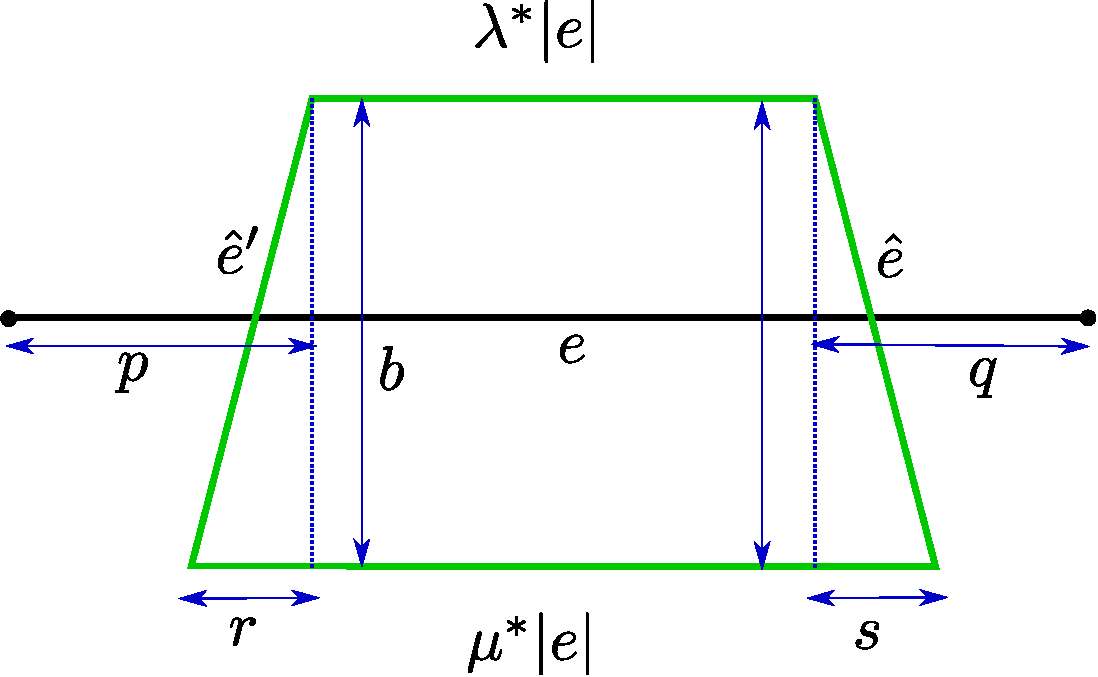
\includegraphics[width=70mm,height=50mm]{eucledian_bound-crop}
	\caption{$4$-gons (green) is a class-$2$ $2$-cell in $\hat{K}$ created around the edge $e$ of input complex $K$.}
	\label{fig:eucledian_bound-crop}
\end{figure}


\subsection{Geometric quality in $d=3$} \label{ssec:qual3d}

We specify how the aspect ratios of $3$-cells of Classes \ref{3dETcls1} and \ref{3dETcls2} compare with those of cells in $K$.
Deriving similar bounds for quality measures of Class \ref{3dETcls3} and \ref{3dETcls4} cells appears more challenging, and is left as part of future work.
In $d=3$, we let the user specify the mitered offset distance $b$ by which each facet (polygon) of a $3$-cell $t \in K$ is moved in to create the corresponding offset cell $\htt \in \hK$.

\subsubsection{Class \ref{3dETcls1} cell}
Let $D, \hD$ denote the diameters, and $\rho, \hrho$ the inradii of cells $t, \htt$, respectively.
Since the Class \ref{3dETcls1} $3$-cell $\htt$ is created as a mitered offset of $3$-cell $t \in K$, we have $~\hD \leq D~$ and $~\hrho \geq \rho - b$.
Hence we get that
\[
\g(\htt) = \frac{\hD}{\hrho} < \frac{D}{\rho - b} = \frac{\g(t)}{\left( 1 - \frac{b}{\rho}\right)}, ~\mbox{ with } \frac{b}{\rho} < 1 \, .
\]
Note that this is the same bound satisfied by the aspect ratio of a Class \ref{2dETcls1} polygon specified in \cref{eq:2dETcls1ar}.
\subsubsection{Class \ref{3dETcls2} cell}
In general, the Class \ref{3dETcls2} $\htt_f$ generated by facet $f \in t \in K$ could have the shape of an ``oblique'' truncated cone with $\hf,\hf'$ as the bases (unlike the ``orthogonal'' truncated cone that \cref{fig:3dETcls2} might indicate).
let $\bar{D}=D+D'$ be the diameter of a ball that contains both $3$-cells $t,t'$ that share $f$ as a facet.
Let $\hat{r}, \hat{r}', r$ be the inradii  of facets $\hf, \hf', f$, respectively, and let $b, b'$ be the offset distance for $f, f'$.
Assume without loss of generality that $\hat{r} < \hat{r}'$.
We can fit an oblique cylinder of radius $\hat{r}$ and height $b + b'$, as shown in \cref{fig:3dETcls2gq}, inside $\htt_f$.
Then we can fit a ball of radius $R = \min\{ \frac{b+b'}{2}, \hat{r}\} \cos{\theta}$, where $\theta$ is the skew angle of the oblique cylinder.
Note that $\theta = 0$ if $\htt_f$ is an ``orthogonal'' truncated cone, in which case the cylinder will be normal as well.
We get
\[\g(\htt_f) = \frac{\hD}{\hrho} \leq \frac{\bar{D}}{R} \,.\]
\begin{figure}[htp!]
      \centering
      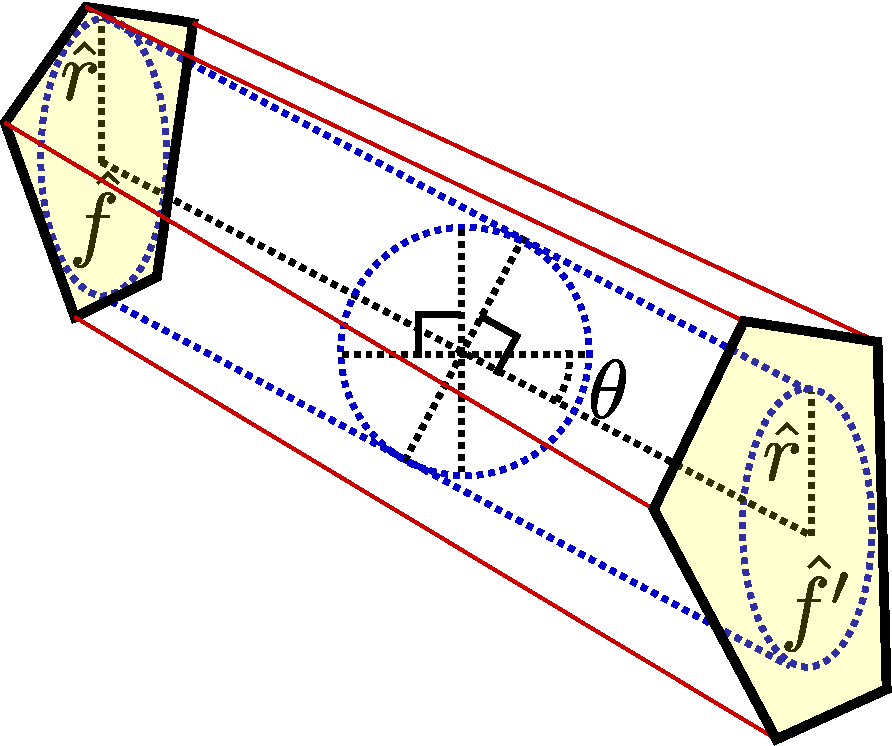
\includegraphics[scale=0.35]{3d_class_2_cell_gq_fig_1_edit-crop}
      \caption{The oblique cylinder we could fit within a Class \ref{3dETcls2} cell $\htt_f$, and the parameters that determine its aspect ratio.
      }
      \label{fig:3dETcls2gq}
\end{figure}



\section{Application: Additive Manufacturing} \label{sec:3dprtg}

We have been using the Euler transformation for tool-path planning in large scale additive manufacturing (3D printing) with our collaborators in Oak Ridge National Laboratory (ORNL).
The system ORNL is developing is termed Big Area Additive Manufacturing (BAAM), and its goal is to be able to \emph{efficiently} print 3D objects that are much larger than the ones that typical 3D-printers in the market today are able to handle (think a few to several feet in each dimension).
Being able to print all edges in a contiguous manner is critical for efficiency.

We present brief details of a proof-of-concept print of a pyramid, which was represented as a collection of planar layers stacked from the ground up (see the left image in \cref{fig:3dprtg}).
The dimensions of the pyramid were $609.6\,$mm $\times$ $609.6\,$mm $\times$ $609.6\,$mm, and each layer had a height of $4.26\,$mm, resulting in a total of $143$ layers.
We started with a standard triangulation $K_0$ of the bottom layer, and obtained the Euler transformation $\hK_0$.
Given the geometry of this object, we took the intersection of $\hK_0$ with the domain of each subsequent layer $i>0$, trimming any vertices and edges of $\hK_0$ that were outside the layer's domain to create $\hK_i$.
This process created some odd-degree nodes at the boundary in $\hK_i$.
But we can show that the number of odd degree nodes in $\hK_i$ is even, and hence we added a set of edges along the perimeter of the layer connecting pairs of odd-degree nodes.
With this modification, $\hK_i$ is guaranteed to be Euler again.

For printing each layer, we used a blossom algorithm to identify an Eulerian tour.
Starting from any vertex, we choose edges at each step that minimize sharp turns in a greedy manner to identify the tool path.

The method outlined above naturally handles voids in the print domain.
We are developing various classes of efficient algorithms for additive manufacturing in this fashion that are capable of incorporating several physical and material constraints.
One such framework has been presented in a separate manuscript \cite{GuKrDr2020}.


\begin{figure}[htp!]
  \centering
  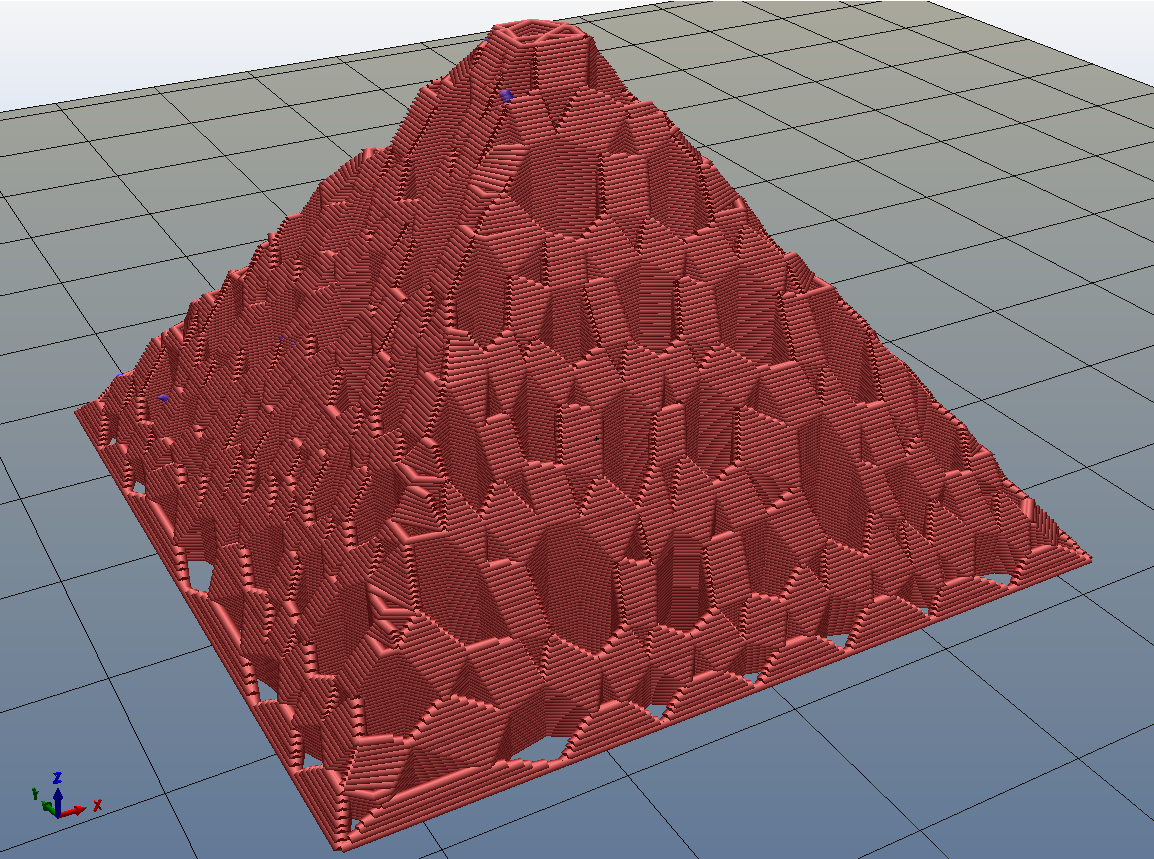
\includegraphics[width=0.45\textwidth]{PyramidPlan}
  \quad
  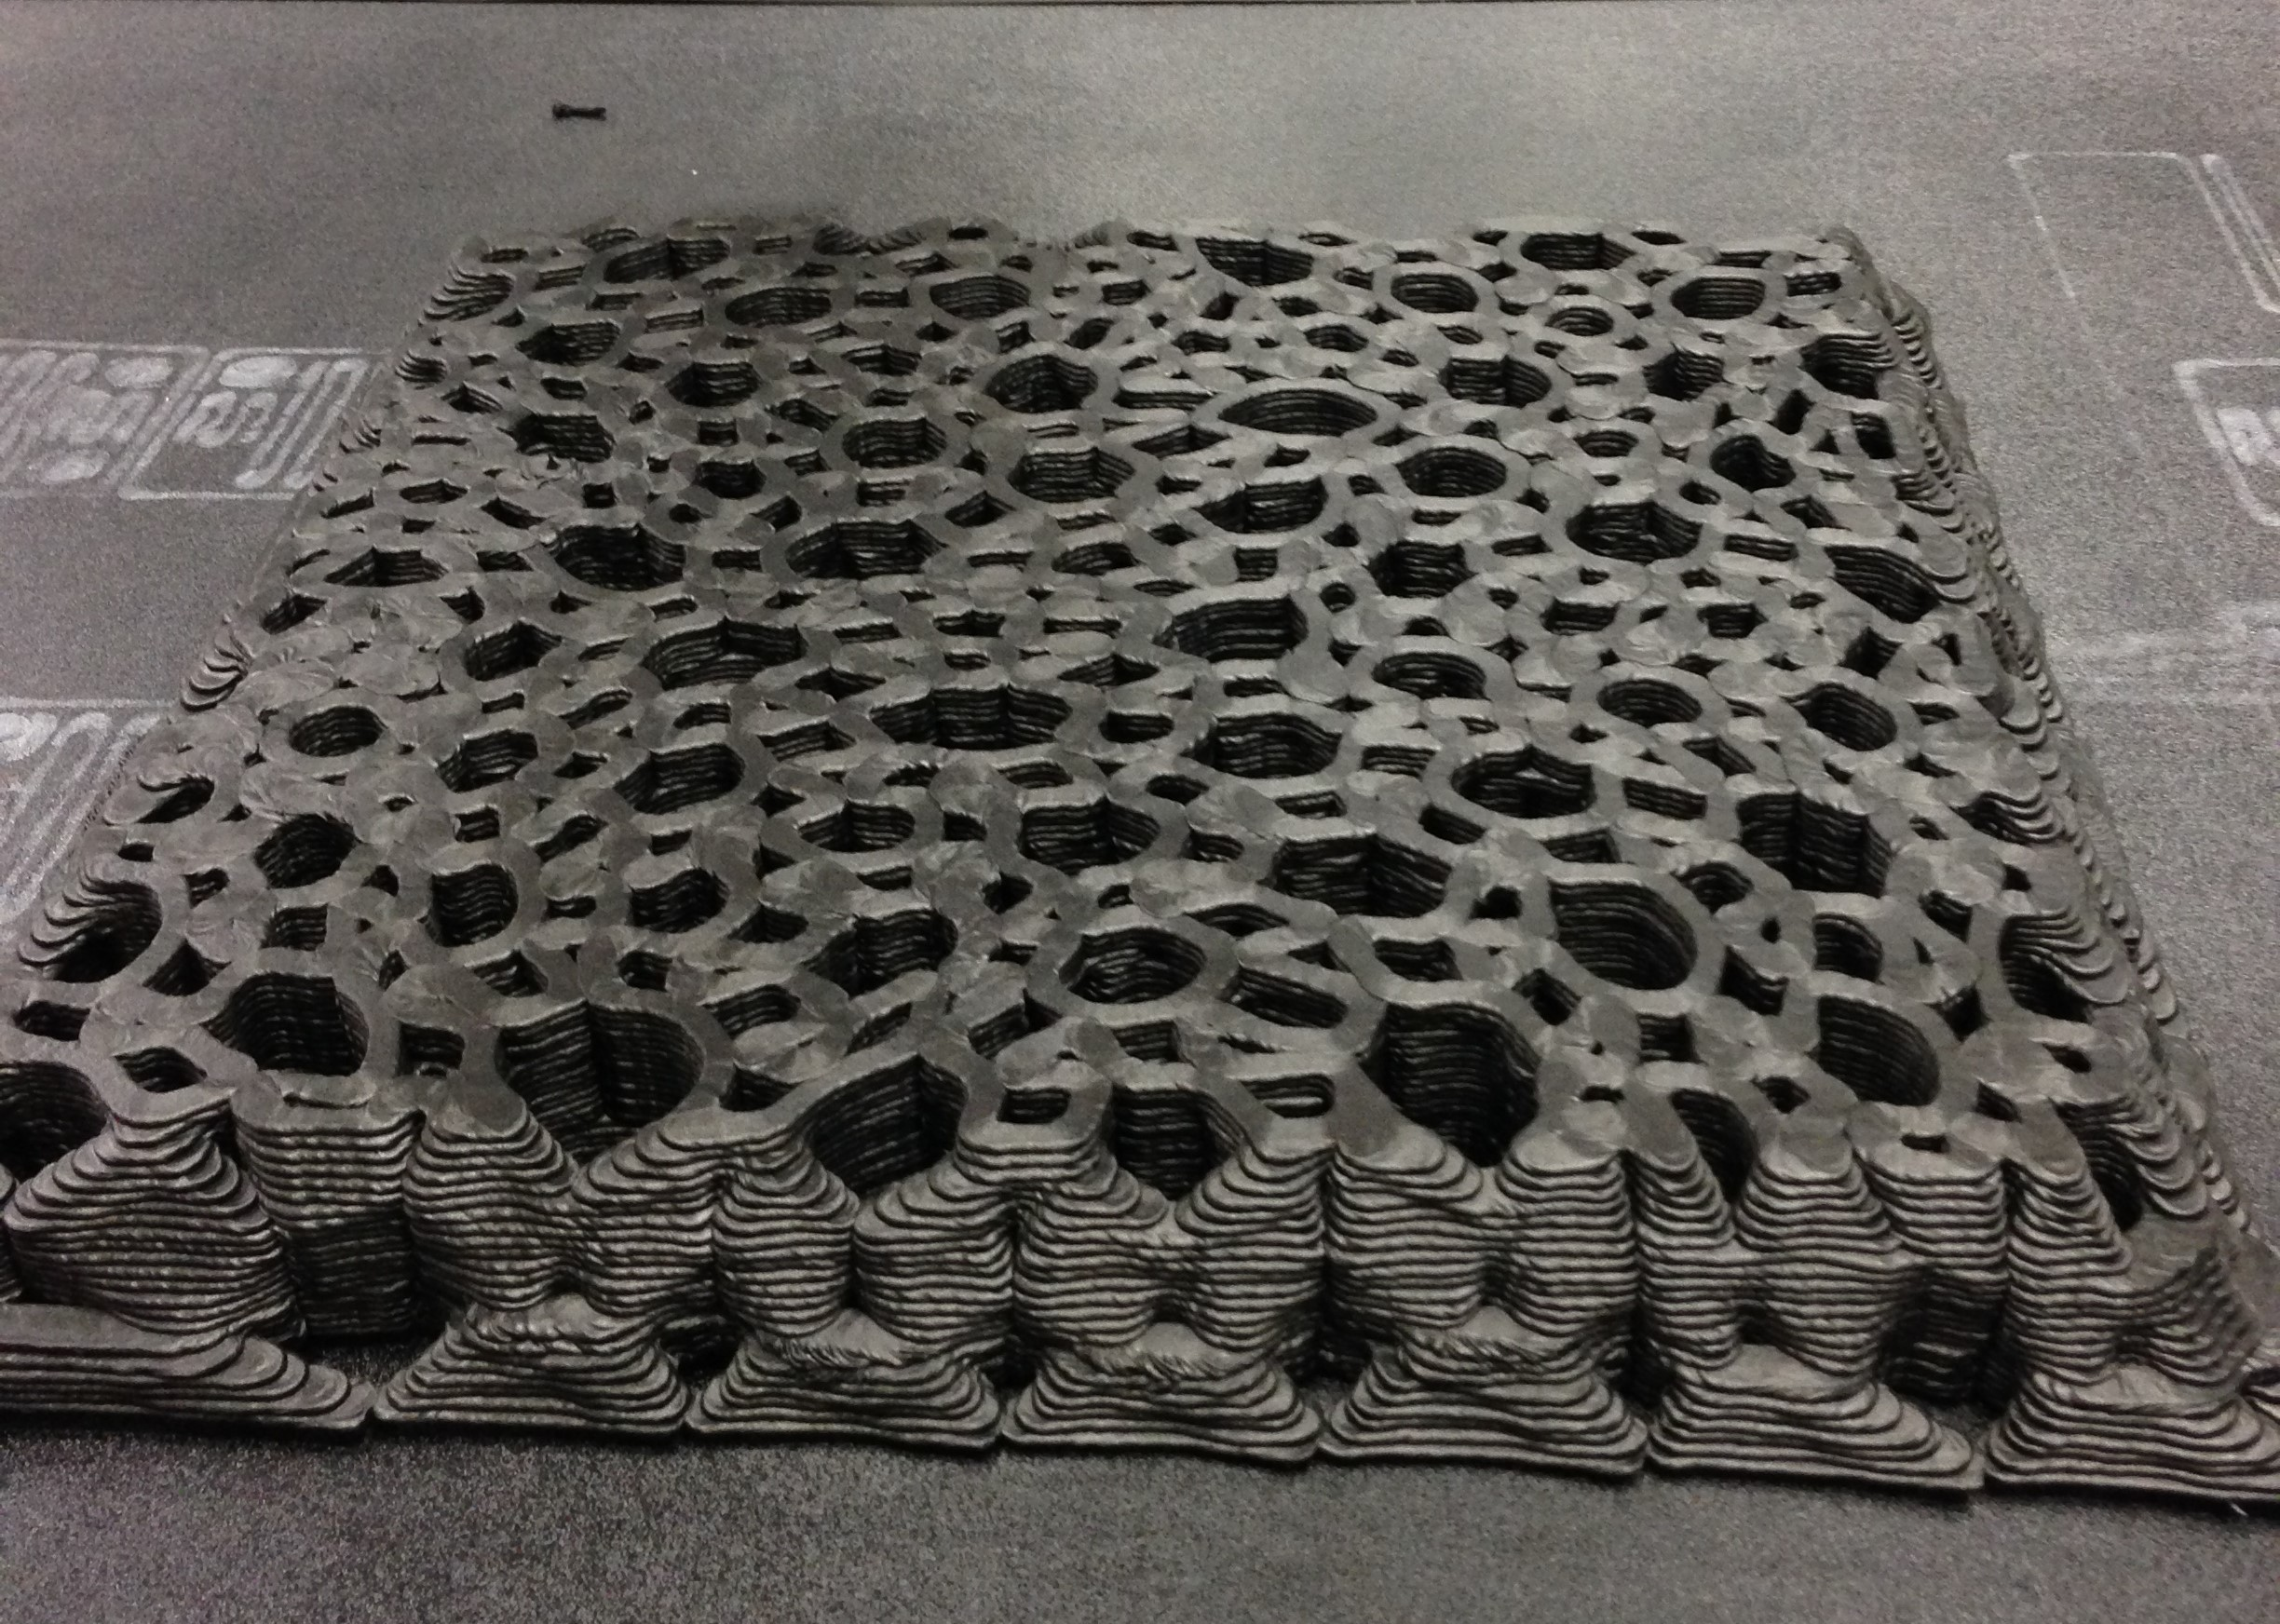
\includegraphics[width=0.47\textwidth]{PrintedPyramid}
  \caption{Visualization of the design of a pyramid-shaped object (left), and a view of the partially 3D-printed object (right). }
  \label{fig:3dprtg}
\end{figure}


\section{Discussion} \label{sec:disc}

The bottleneck for computational complexity of the Euler transformation is determined by the mitered offsets it creates for each cell in $K$.
The number of cells in $\hK$ are clearly linear in the number of cells in $K$ (\cref{lem:cntshVhEhF2d,lem:cntshThVhEhf3d}).
For $d=2,3$, if $K$ in $\R^d$ has $m$ $d$-cells, each of which has at most $p$ facets, the time complexity of Euler transformation is $O(m p^d)$ \cite{AuWa2013,AuWa2016}.

Not all cells in the Euler transformation $\hK$ are guaranteed to be convex, even when all cells in $K$ are (see \cref{fig:disjholes}).
%We could triangulate the non-convex cells so that all cells in $\hK$ are convex.
%But could we do so while maintaining even degrees for all vertices?
%A related problem is that of finding a triangulation (rather than a cell complex) of a given domain that minimizes the number of odd-degree vertices.

We pointed out in \cref{rem:nonplnr3d} that Class \ref{3dETcls3} or \ref{3dETcls4} cells in $\hK$ might have nonplanar facets (in $d=3$).
We suggested not including these $3$-cells in $\hK$ when we are more interested in its $1$-skeleton.
%But if we want to ensure $\hK$ is indeed a cell complex, we could consider triangulating the nonplanar facets.
%Again, could we do this triangulation while maintaining even degrees for all vertices in $\hK$?
%We may be able to do so if each edge $e \in K$ is shared by the same number of $3$-cells.

%%%%%%%%%%%%%%%%%%%%%%%%%%%%%%%%%%%%%%%%%%%%%%%%%%%%%%%%%%%%%%%%%%%%%%%%%%%%%%%


  \chapter{Continuous Toolpath Planning in Additive Manufacturing}

\section{Introduction} \label{sec:introadditiv}

\emph{Additive manufacturing} refers to any process that adds material  to create a 3D object. %
3D printing is a popular form of additive manufacturing that deposits material (plastic, metal, biomaterial, polymer, etc.) in layer by layer fashion. % to form the object.
We focus on extrusion based 3D printing, in which material is pushed out of an extruder that follows some tool path while depositing material in beads that meld together upon contact.
In this paper, we will refer to this process simply as 3D printing.


In most 3D printing jobs, we first print the outer ``shell'' or boundary of the 3D object in each layer.
We then cover the interior space by printing an \emph{infill lattice} \cite{WuAaWeSi2018}, which is typically a standard mesh. % \cite{BrBrWiHa2012},
In an arbitrary infill lattice, one is not guaranteed to find a \emph{continuous} tool path, i.e., an entire layer being printed by non-stop extrusion of material.
Non-continuous tool paths typically have multiple starts and stops, which could reduce quality of the print, cause print failures (e.g., delamination), and could increase print time.
To ensure existence of a continuous tool path, we need to choose the mesh modeling the infill lattice carefully.
Subsequently, we need to develop algorithms that ensure a continuous tool path can be obtained for each layer with arbitrary geometry.
Further, we need to identify a traversel of this tool path that avoids crossovers.
%We propose an approach to transform any cellular complex under mild assumptions into an \emph{Eulerian} complex.
%Every vertex in the $1$-skeleton (i.e., graph) of an Eulerian complex has an even degree, and hence a continuous tool path is guaranteed to exist.

\subsection{Our contributions} \label{ssec:contribaddit}
We recently proposed a method that transforms a given $2$-dimensional cell complex $K$ into a new $2$-complex $\hK$ in which every vertex is part of a uniform even number of edges \cite{GuKr2018}.
Hence every vertex in the graph $\hG$ that is the $1$-skeleton of $\hK$ has an even degree, which makes $\hG$ Eulerian, i.e., it is guaranteed to contain an Eulerian tour.
We refer to this method as an \emph{Euler transformation} of a polygonal (or cell) complex.
%We first describe the Euler transformation of a $2$-complex \emph{abstractly}.
For the sake of completeness of the present paper, we present details of the Euler transformation in 2D here.
For $2$-complexes in $\R^2$ under mild assumptions (that no two adjacent edges of a polygon in $K$ are boundary edges), we show that the Euler transformed $2$-complex $\hK$ has a geometric realization in $\R^2$, and that each vertex in its $1$-skeleton has degree $4$.
We bound the numbers of vertices, edges, and polygons in $\hK$ as small scalar multiples of the corresponding numbers in $K$.
\begin{comment}
We prove corresponding results for $3$-complexes in $\R^3$ under an additional assumption that each vertex in $K$ is connected to three edges in a $3$-cell that contains the vertex, i.e., the degree of each vertex in the $1$-skeleton of each $3$-cell in $K$ containing the vertex is $3$.
In this setting, every vertex in $\hG$ is shown to have a degree of $6$.
Next, we presents bounds on parameters measuring geometric quality (aspect ratios) of $\hK$ in terms of the corresponding parameters of $K$ (for $d=2$).
One can control these quality measures by choosing user-defined offset parameters appropriately.
\end{comment}

We present a computational framework for 3D printing that identifies continuous tool paths for printing the infill lattice in each layer. We illustrate the steps in our framework in Figure \ref{infill_pattern_work_flow} (on a 3D pyramid with a square base).
First we find the polygons for each layer of the input 3D domain (typically presented as an STL file, e.g., Figure \ref{pyramid})) using a slicing software.
Let $\Ps$ be the union of all of these polygons in 2D (Figure \ref{union_of_projections}). 
We fill the space in $\Ps$ with some infill lattice $K$, using any meshing algorithm (Figure \ref{infill_pattern}).
We then apply Euler transformation to obtain a new infill lattice $\hK$ that is guaranteed to be Euler (Figure \ref{infill_pattern_transformed}).
In the next step, we \emph{clip} $\hK$ using $P_i$, a polygon in layer $i$ (Figure \ref{infill_pattern_transformed_polygon_cut}).
Depending on the shape of $P_i$, this step could create terminal vertices in the infill lattice for layer $i$, making it no longer Euler.
In the last step, we \emph{patch} the clipped infill lattice by adding new edges such that the resulting infill lattice is Euler again (Figure \ref{infill_pattern_transformed_polygon_patch_simple}).
An application of this framework is illustrated in Figures \ref{pyramidplan} and \ref{printedpyramid}.
Finally, we propose a tool path algorithm (Section \ref{sec:toolpathalgo}) that identifies the actual print tool path from the patched Euler infill lattice that avoids crossovers and material collisions.
We address all geometric/computational challenges that arise along the way to ensure the proposed framework is complete.
Since each layer can have multiple polygons in general, our framework can generate continuous tool path for each polygon in a given layer (see Section \ref{sec:boundaryedges} for an exception arising in certain cases with extreme geometries).
As we might not print every boundary edge after the patching step, we also print \emph{support} edges (see Section \ref{sec:slicing}).
The overall goal of our framework is to create an Euler infill lattice in each layer, and also prevent printing in free space so as to avoid print failures.
We are currently investigating the implementation and testing of our algorithmic framework for 3D printing in detail, and plan to present details in an uncoming paper.

\begin{figure}[htp!]
  \centering
%\hspace*{0.15in}
  \begin{subfigure}[t]{1.7in}
    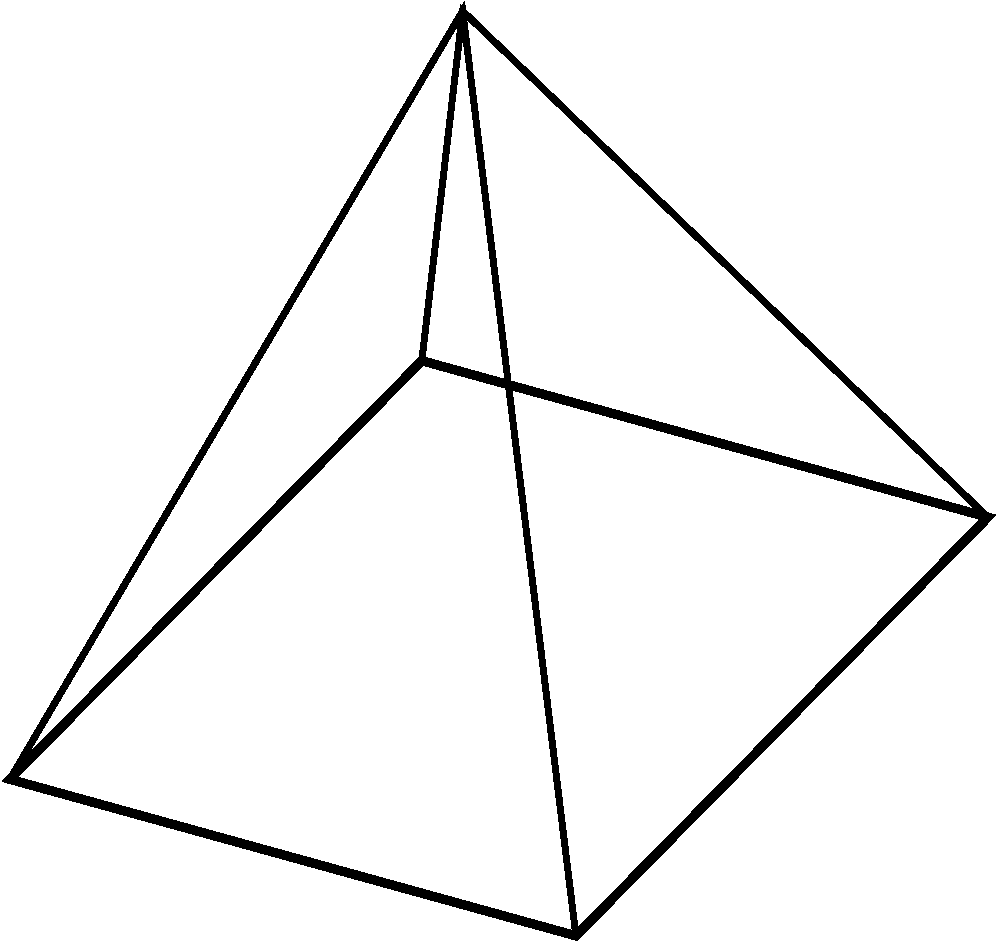
\includegraphics[scale=0.25]{pyramid_crop}
    \caption{\small \label{pyramid}}
  \end{subfigure}
%\hspace*{0.15in}
  \begin{subfigure}[t]{1.7in}
    
\includegraphics[scale=0.25]{union_of_projections_crop}
    \caption{\small \label{union_of_projections}}
  \end{subfigure}
%\hspace*{0.15in}
  \begin{subfigure}[t]{1.7in}
    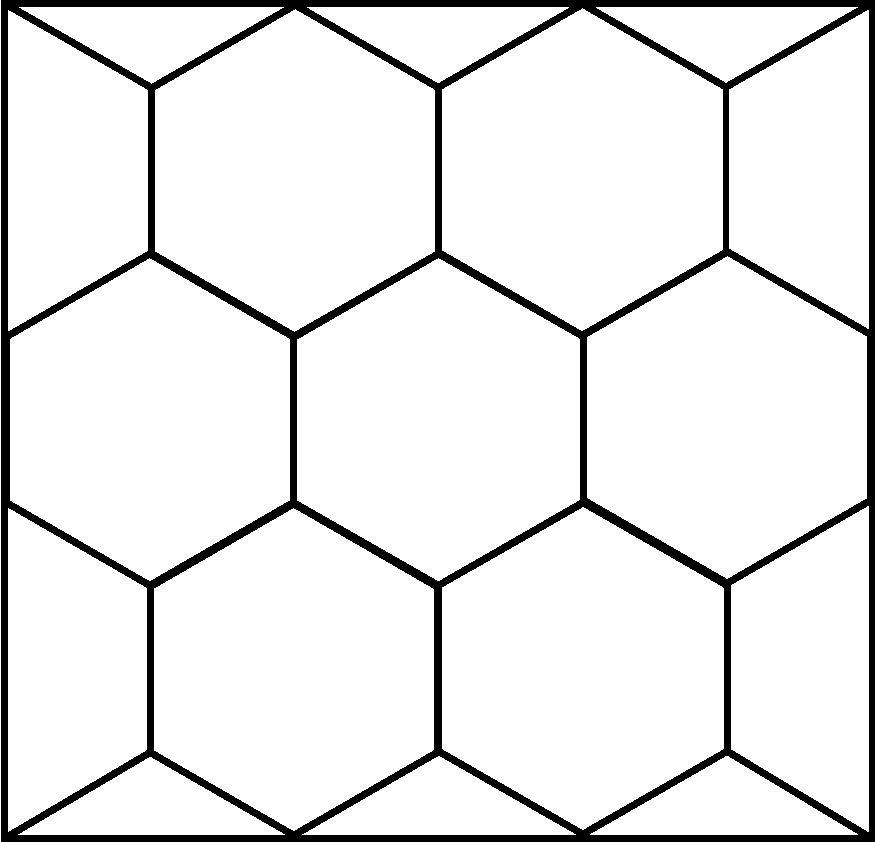
\includegraphics[scale=0.25]{infill_pattern_crop}
    \caption{\small \label{infill_pattern}}
  \end{subfigure}
%\hspace*{0.15in}
  \begin{subfigure}[t]{1.7in}
    %\centering
    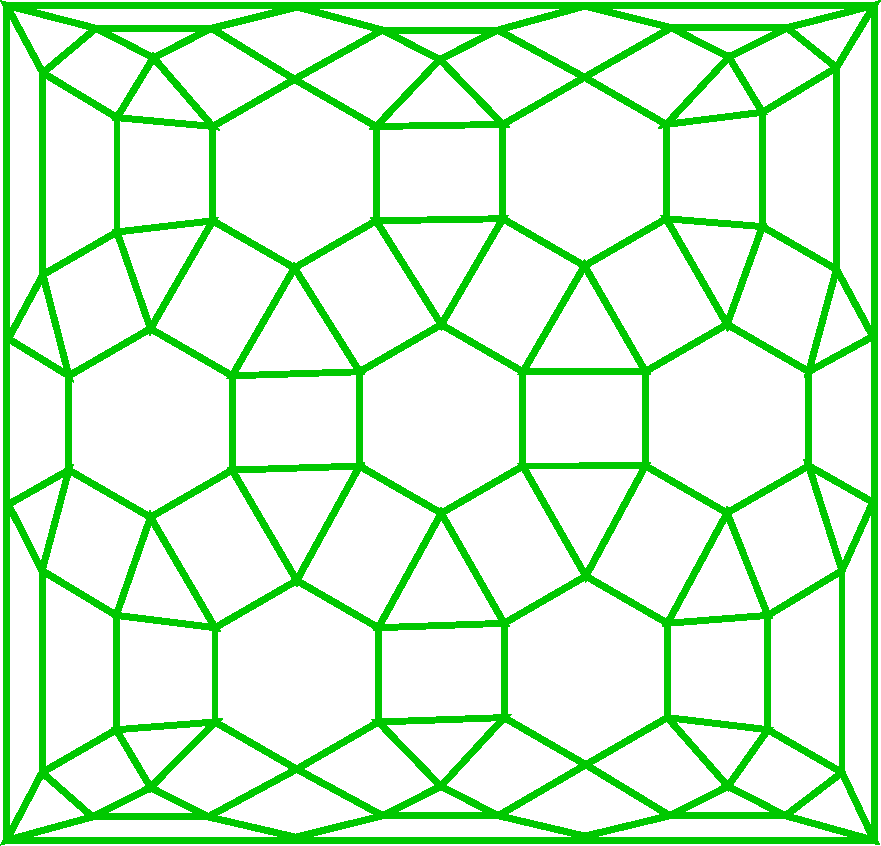
\includegraphics[scale=0.25]{infill_pattern_transformed_crop}
    \caption{\small \label{infill_pattern_transformed}}
  \end{subfigure}
%\hspace*{0.15in}
  \vspace*{0.05in}
  \begin{subfigure}[t]{1.7in}
    %\centering
    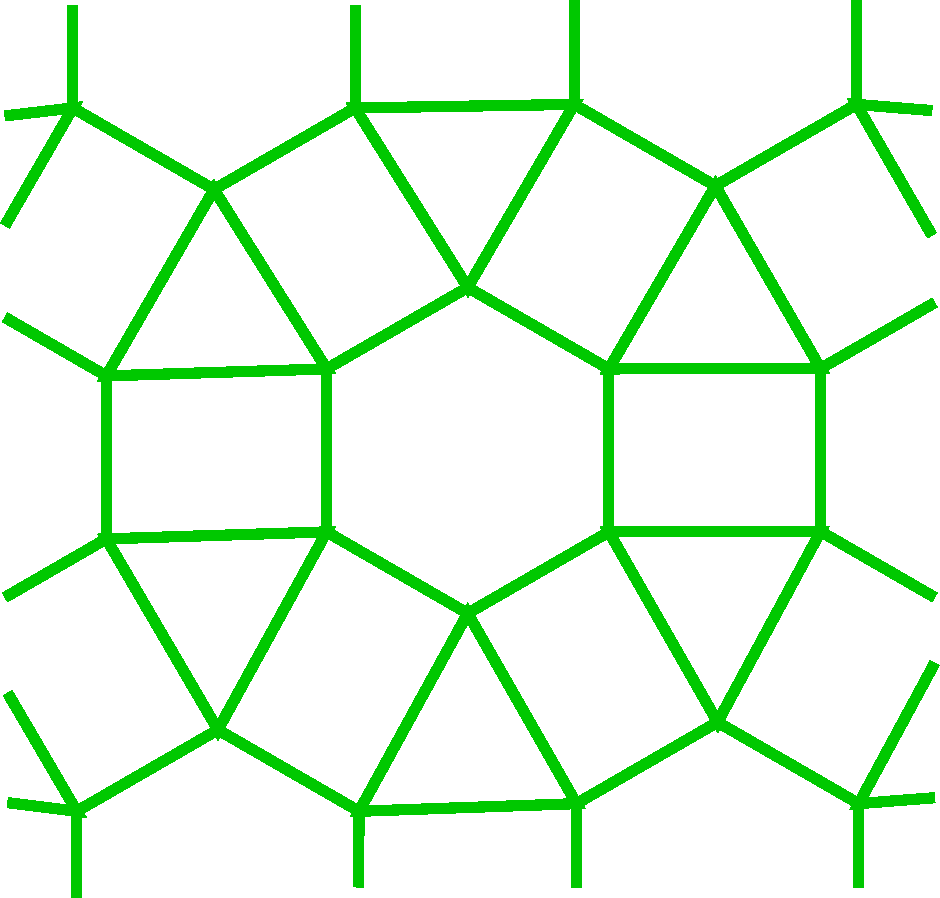
\includegraphics[scale=0.25]{infill_pattern_transformed_polygon_cut_crop}
    \caption{\small \label{infill_pattern_transformed_polygon_cut}}
  \end{subfigure}
%\hspace*{0.15in}
  \begin{subfigure}[t]{1.7in}
    %\centering
    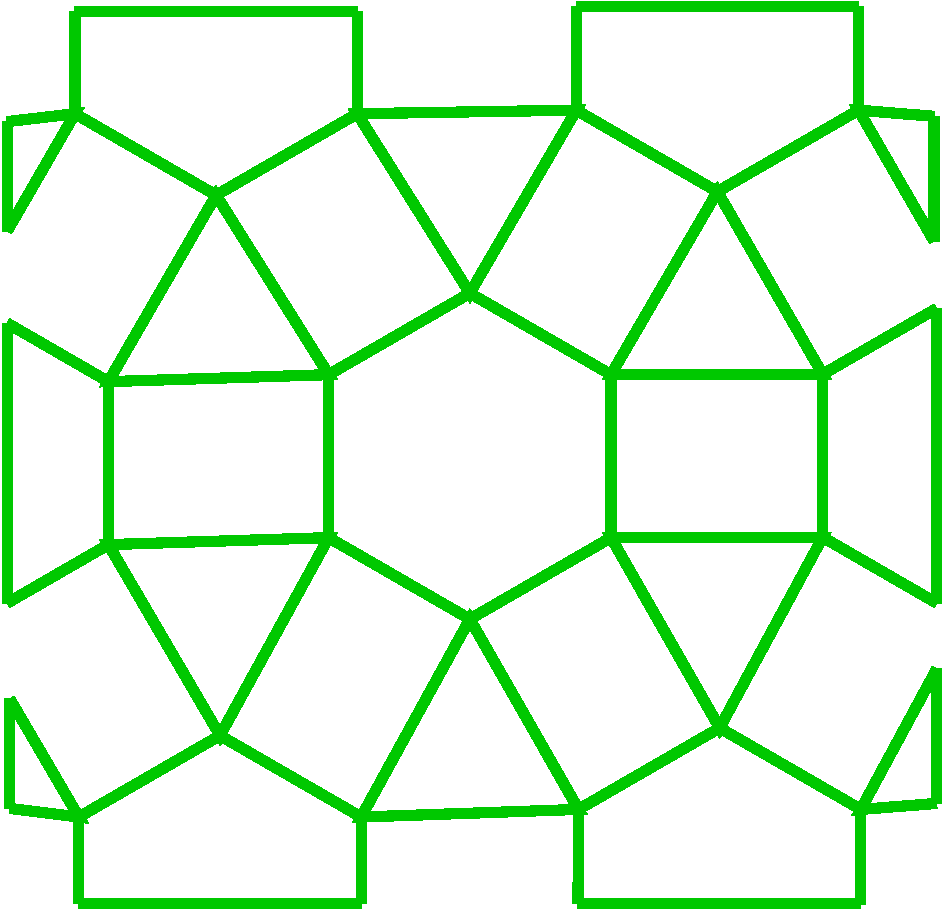
\includegraphics[scale=0.25]{infill_pattern_transformed_polygon_cut_patch_simple_crop}
    \caption{\small \label{infill_pattern_transformed_polygon_patch_simple}}
  \end{subfigure}
  %\vspace*{0.05in}
  %\hspace*{-0.1in}
  \begin{subfigure}[t]{2.5in}
    %\centering
    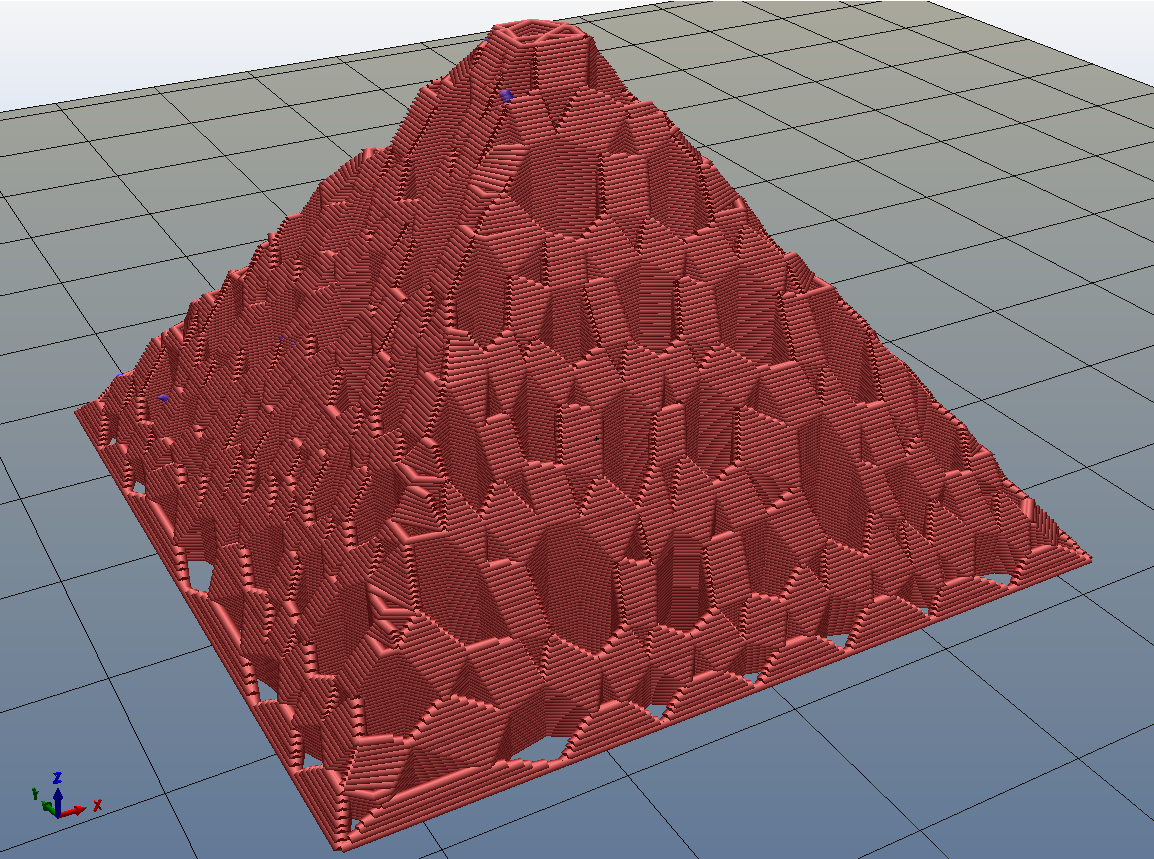
\includegraphics[scale=0.15, bb=0 0 1154 859]{PyramidPlan} 
    \caption{\small \label{pyramidplan}}
  \end{subfigure}
%\hspace*{0.15in}
  \begin{subfigure}[t]{2.5in}
    %\centering
    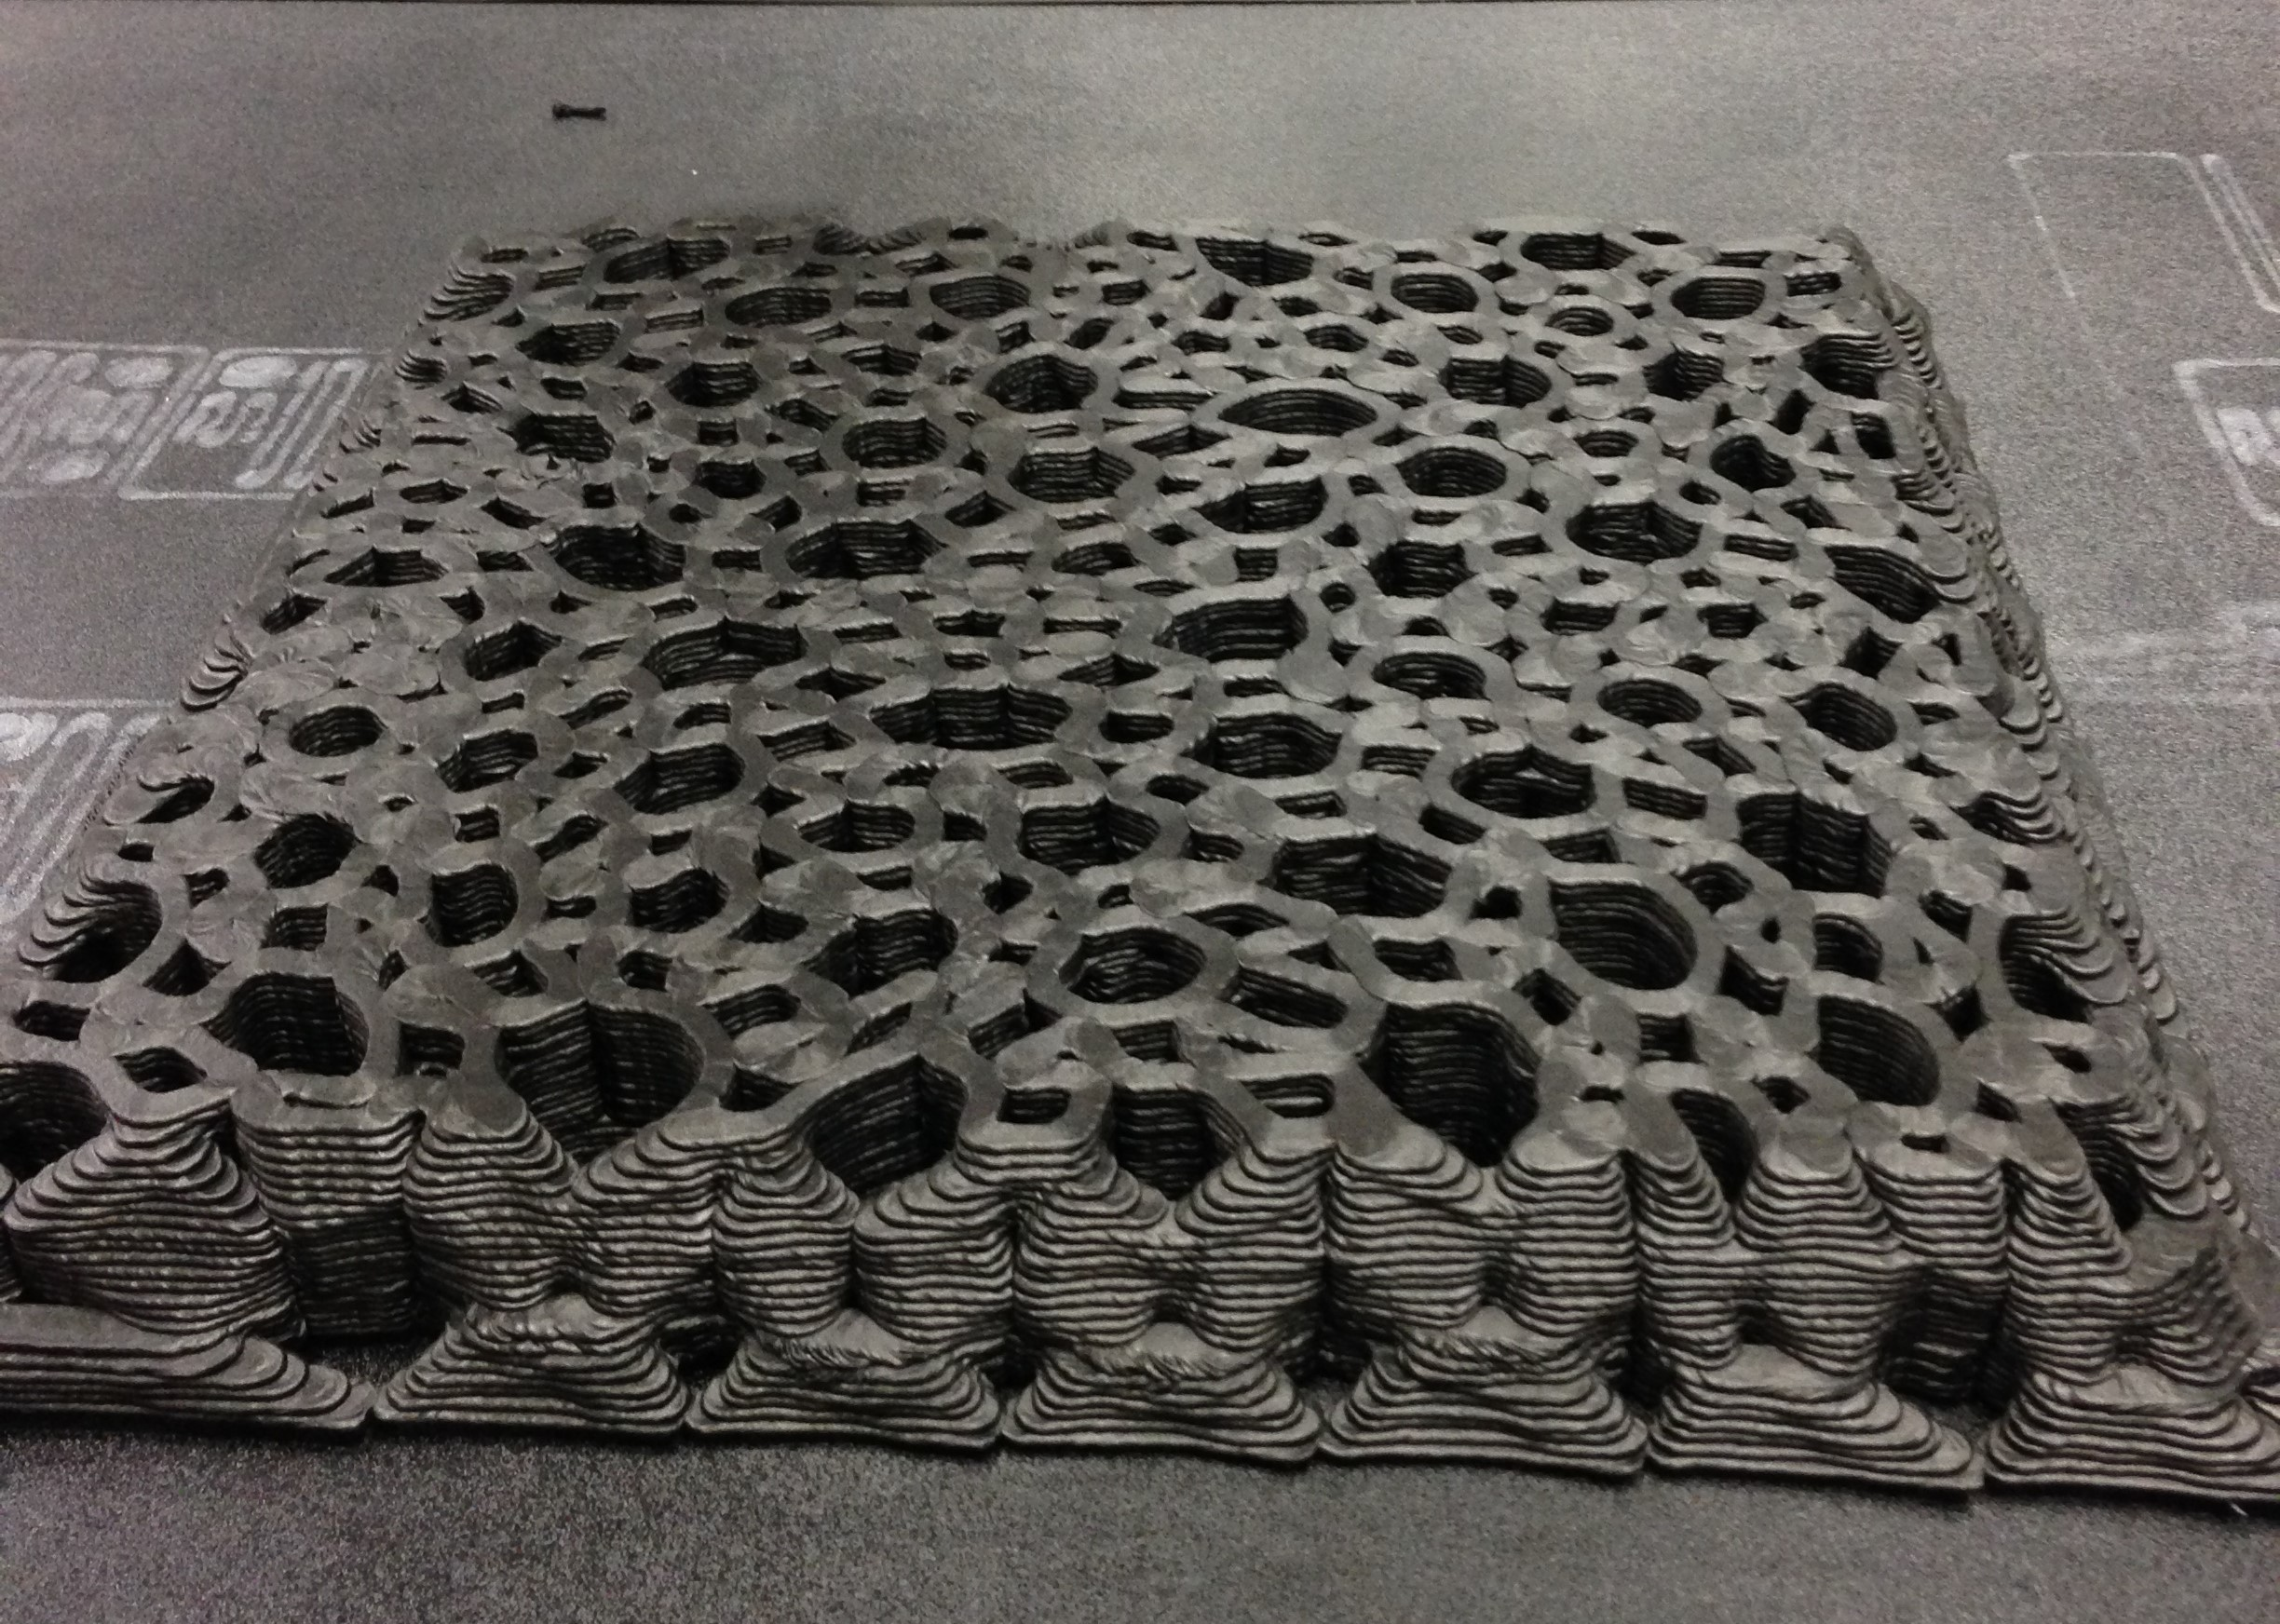
\includegraphics[scale=0.075, bb=0 0 2448 1744]{PrintedPyramid}
    \caption{\small \label{printedpyramid}}
  \end{subfigure}
  %\vspace*{-0.1in}
  \caption{ \label{infill_pattern_work_flow}
    Illustration of our framework (see Section \ref{ssec:contrib} for details).
    Subfigures (g: plan) and (h: mid-print slice) show an implementation for a  $610\,$mm $\times$ $610\,$mm $\times$ $610\,$mm pyramid.
    We plan to present complete details of our implementation in a separate manuscript.
    %\vspace*{-0.1in}
  }
\end{figure}

\subsection{Related work}

%\input{Journal_prior_ET2d}

%\input{SCF_backg3d}
%\subsection{Euler Graph} \label{sec:previouseulerwork}
\paragraph{Euler Graph.} \label{sec:previouseulerwork}
The $1$-skeleton of $K$ is an undirected planar graph ($G$).
One approach to make $G$ Eulerian is to delete a minimal number of vertices and/or edges.
But Cai and Yang~\cite{CaYa2011} showed that the Euler vertex deletion and Euler edge deletion problems are NP-Complete.
More importantly, removing edges and/or vertices could create gaps in the coverage of the domain, potentially affecting the mechanical properties of the final product.
Another approach to make $G$ Eulerian is to add a minimum number of edges that pair odd degree vertices in $G$, which can be cast as a \emph{graph augmentation} problem.
Boesch~\cite{TCR1977} presented a polynomial time algorithm for this problem, but planarity of $G$, which is necessary to avoid material collision, is not guaranteed after the augmentation.
Another approach for augmentation is to use the Chinese postman problem to double the edges along shortest paths connecting odd degree vertices in $G$.
But printing the resulting multigraph could be challenging due to non-uniform thickness of (multiple copies of) edges and non-uniform degrees of nodes.
In fact, the degree of some of the nodes could be multiplied by up to $n^o/2$, where $n^o$ is the number of odd degree vertices in $G$.
Visiting a vertex a large number of times could reduce quality of the print.

Jin et al.~\cite{JiHeFuZhDu2017} showed that subpaths in this setting could be generated using a geometric approach and then joined optimally to reduce the amount of jumps.
And Zhao et al.~\cite{ZhGuHuGaYoChBeZhCoDaBa2016} proposed a method that can find global continuous paths using Fermat spirals.
But both of these approaches are designed for completely filling the region (with or without holes), and not for sparse infilling.
   
The Catmull-Clark subdivision \cite{CatmullClark1978} creates quadrilateral polygons from any input $2$-complex.
But some vertices in the resulting mesh may have odd degrees.
% it may produce Hence may have some vertices with odd degree or even degree with at least degree $6$. Odd degree vertices creates discontinuous print path in case every edge in $1$-skeleton of the complex must be printed.
%Analogous to Catmull-clark subdivision scheme Bajaj el at \cite{ChJoGu2001} developed a hexahedral $3$-cell $3$-complex for any arbitrary $3$-complex, where vertices in $3$-cell has degree $3$. Similarly there may be some extraordinary vertices with odd degree.

Our Euler transformation appears similar to the Doo-Sabin subdivision \cite{DoSa1978},
%But Doo-Sabin could produce odd degree vertices on the boundary of the domain, the underlying space is not preserved, and copies of cells retained from the original complex may not preserve interior angles.
%Further, positions of new vertices in the Doo-Sabin subdivision are strictly prescribed, making it hard to control quality of the mesh.
%Finally, combinatorial changes of cells retained from the input complex are not permitted in this subdivision.  
%The Doo-Sabin subdivision
which creates new vertices for each polygon after $k+1$ iterations specified as
\[v_i^{k+1} = \sum_{j =1}^{n} a_{ij} v_j^{k}, ~~\mbox{ where }\]
\[a_{ii} = \frac{n + 5}{4n} ~\mbox{ and }\] 
\[a_{ij} = \frac{3 + 2 \cos(2\pi\frac{(i -j)}{n})} {4n}, \] 
where $n$ is number of vertices of the polygon and $\sum_{j=1}^{n}a_{ij} = 1$.
We outline key differences between the Doo-Sabin and our Euler transformation below.    
\begin{itemize}
  \item
    Doo-Sabin subdivision does not preserve the underlying space, and creates boundary vertices with odd degree, as shown in Figure \ref{fig:exampdooeulercombinat}.
    It will add $O(b)$ jumps, where $b$ is the number of boundary vertices after subdivision.%\add{What are the units of this retraction?}   
  \item
    New vertices are created in the Doo-Sabin subdivision based on vertices and the number of edges in the original polygon.
    But in our Euler transformation, new vertices are created through mitered offsets (parallel offset of neighboring edges) of polygons as shown in the Figure \ref{fig:exampdooeulercombinat}.
    Suppose $e_{ij}^1$ is an edge created in a polygon after the first iteration of Doo-Sabin.
    %Then we have that
    %\[\norm{e_{ij}^1} =  \frac{n + 5}{4n}\norm{e_{ij}^0} = (0.25 + \frac{1.25}{n})\norm{e_{ij}^0}.\]
    %This setting implies that $0.25 \norm{e_{ij}^0} < \norm{e_{ij}^1} < 0.67\norm{e_{ij}^0}$ as $n \geq 3$.
    For large values of $n$, we get that $\norm{e_{ij}^1} \approx 0.25 \norm{e_{ij}^0}$, whereas in our Euler transformation, the edge lengths are flexible as they depend on the mitered offsets chosen rather than on $n$. 

  \item Original angles are not preserved in the Doo-Sabin subdivision, as illustrated in Figure \ref{fig:exampdooeulercombinat}. 

  \item Combinatorial changes are not allowed in the Doo-Sabin subdivision, where as our Euler transformation allows combinatorial changes as shown in Figure \ref{fig:exampdooeulercombinat}.
  Combinatorial changes help in avoiding extremely small edges after transformation (see Section \ref{sec:eulertransformwithcombin}). 

  \item Topological changes are not allowed in the Doo-Sabin subdivision for any concave polygon, whereas our Euler transformation allows topological changes as shown in Figure \ref{fig:exampdooeulertopochang}.
  Since new  vertices are created as convex combinations of original vertices of the input polygon in Doo-Sabin subdivision, the resulting polygon is convex.
  But it will not necessarily be contained in the original polygon.
  Details on topological changes in our Euler transformation is mentioned in Section \ref{sec:eulertransformwithTopolog}.      
\end{itemize}


\begin{figure}[ht!] 
	\centering
	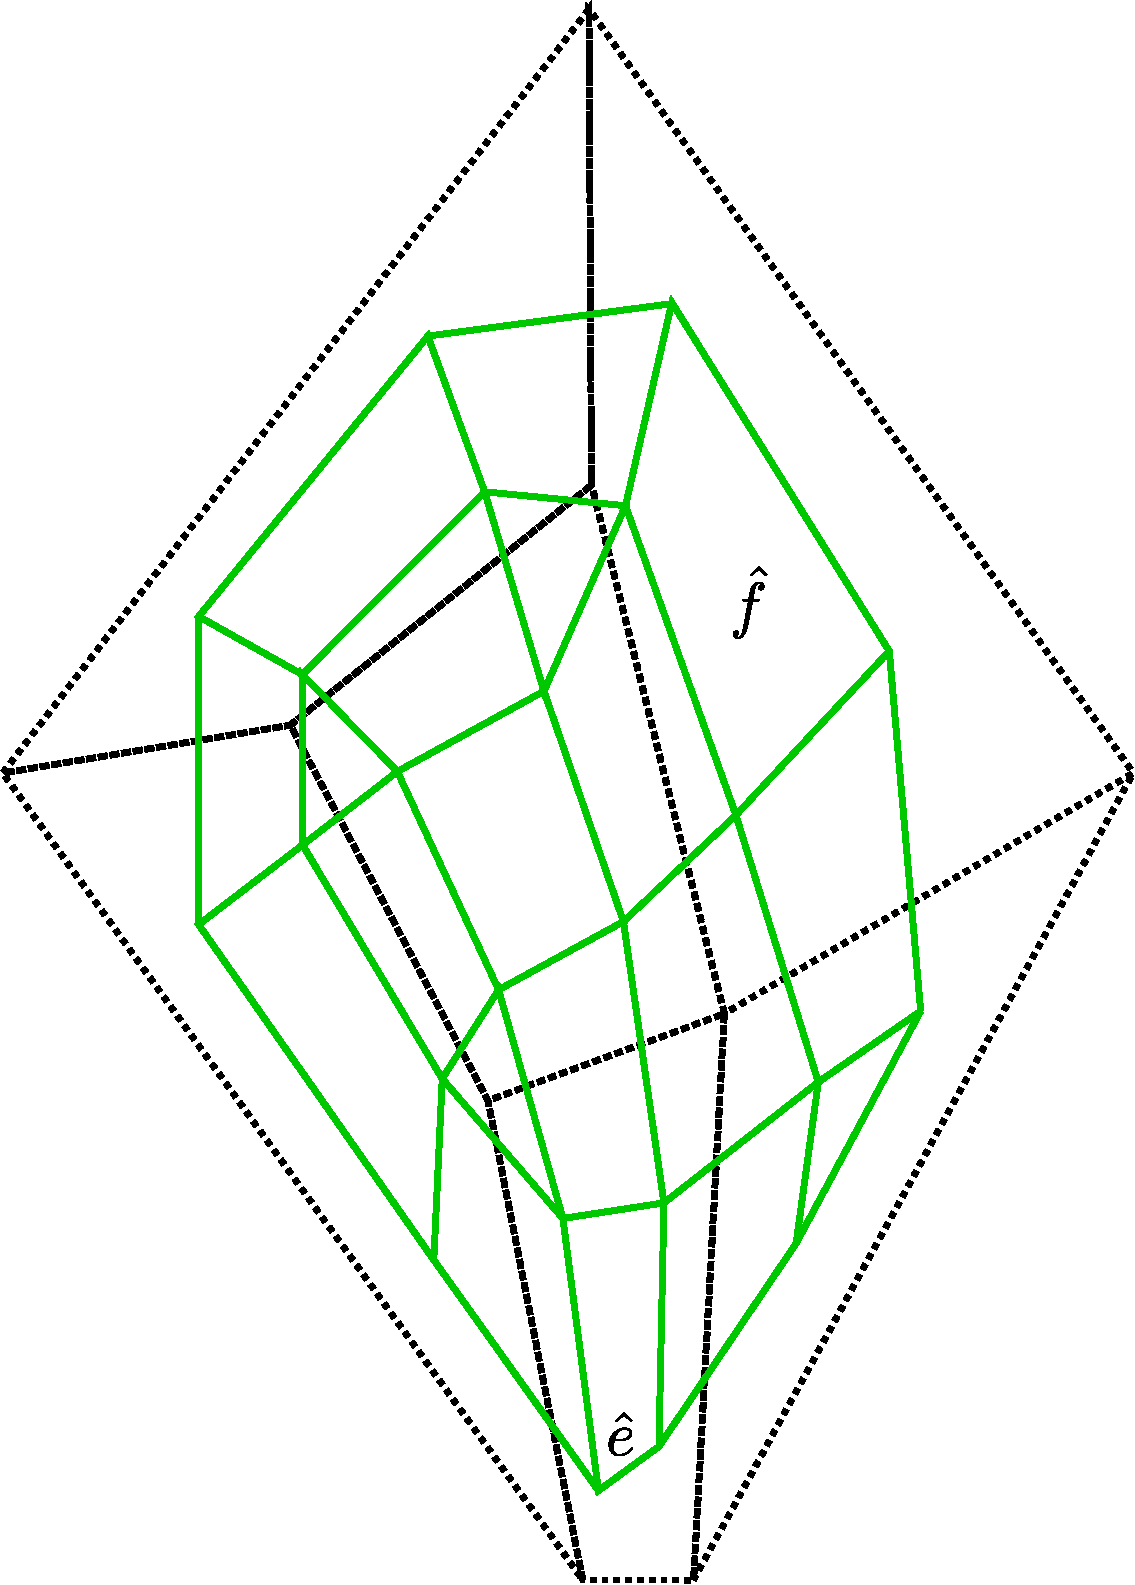
\includegraphics[scale=0.22]{doo_sabin_subdivision_example_1_crop}
	\quad
	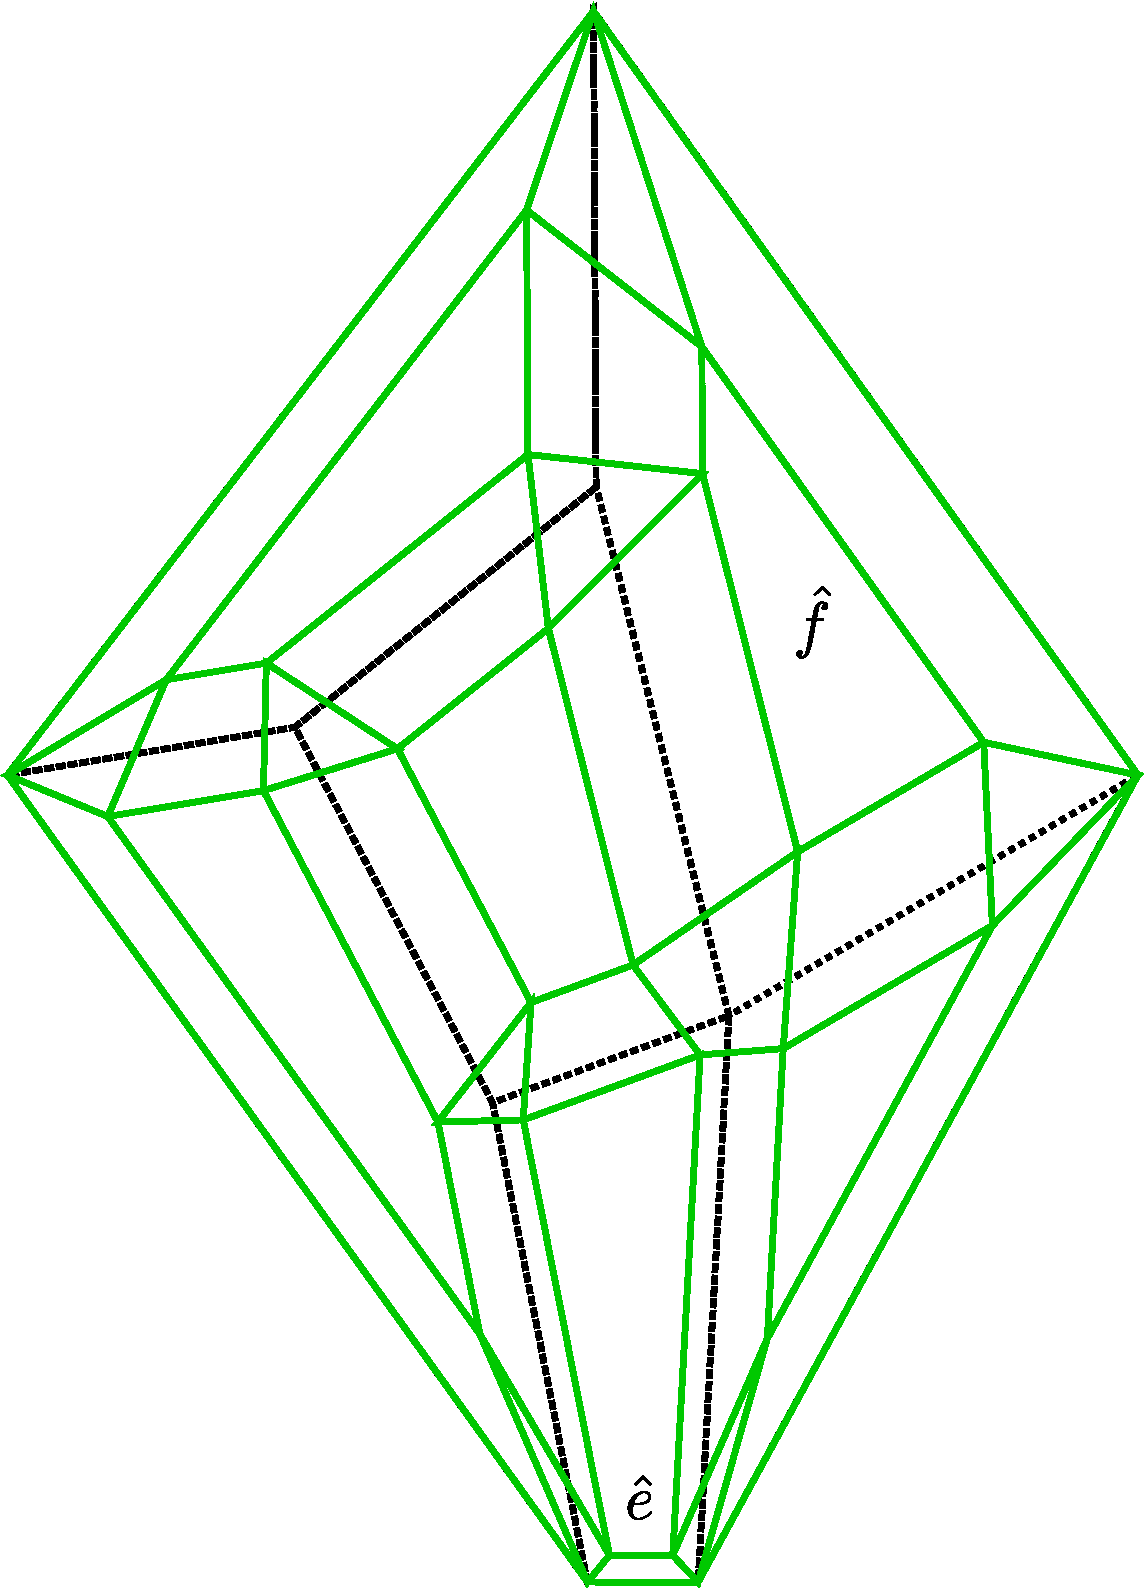
\includegraphics[scale=0.22]{euler_transformation_example_1_crop}
	\quad
	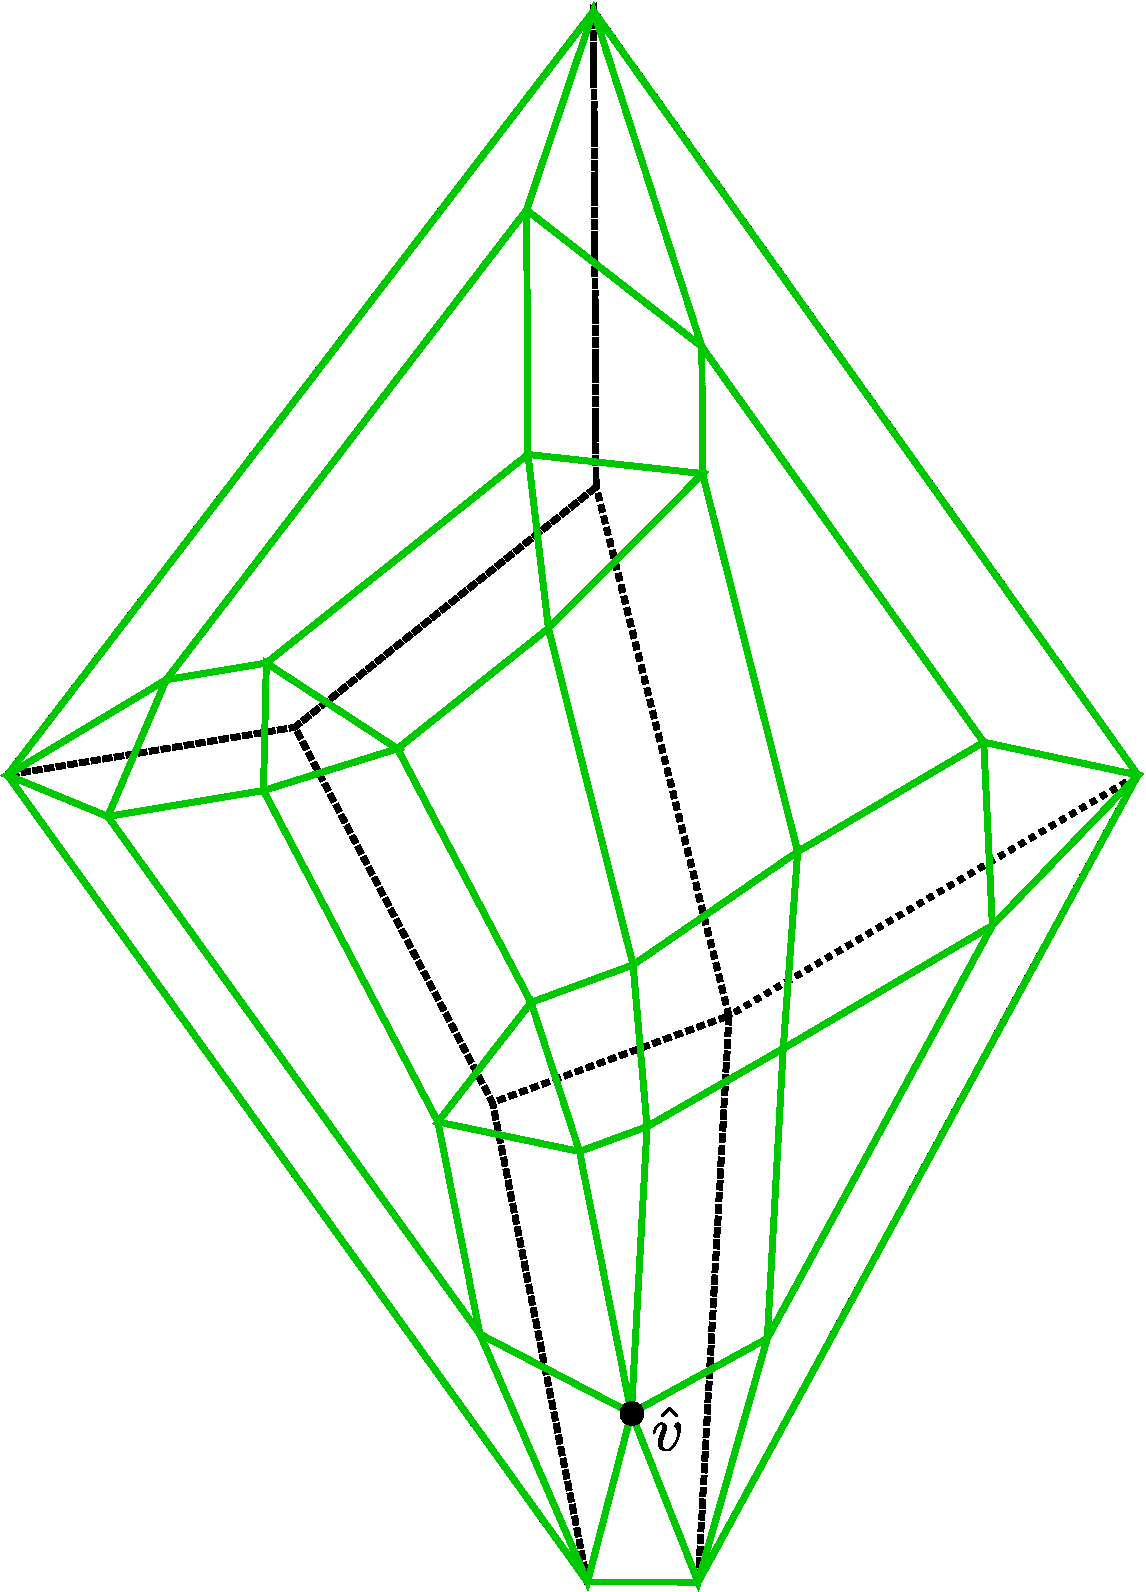
\includegraphics[scale=0.22]{euler_transformation_example_1_combinatorial_changes_crop}
	\caption{\label{fig:exampdooeulercombinat}
        Input complex $K$ (in dotted black) and three different output complexes $\hat{K}$ (in green).
        Doo-Sabin subdivision of $K$ (left), Euler transformation of $K$ without combinatorial changes (middle), and Euler transformation of $K$ with combinatorial changes (right).
        Cell $\hat{f}$ of $\hat{K}$ does not preserve the angles of input complex in the left Figure, but $\hat{f}$ of $\hat{K}$ does preserve the angles in the middle and right Figures. }
\end{figure}

\begin{figure}[ht!] 
	\centering
	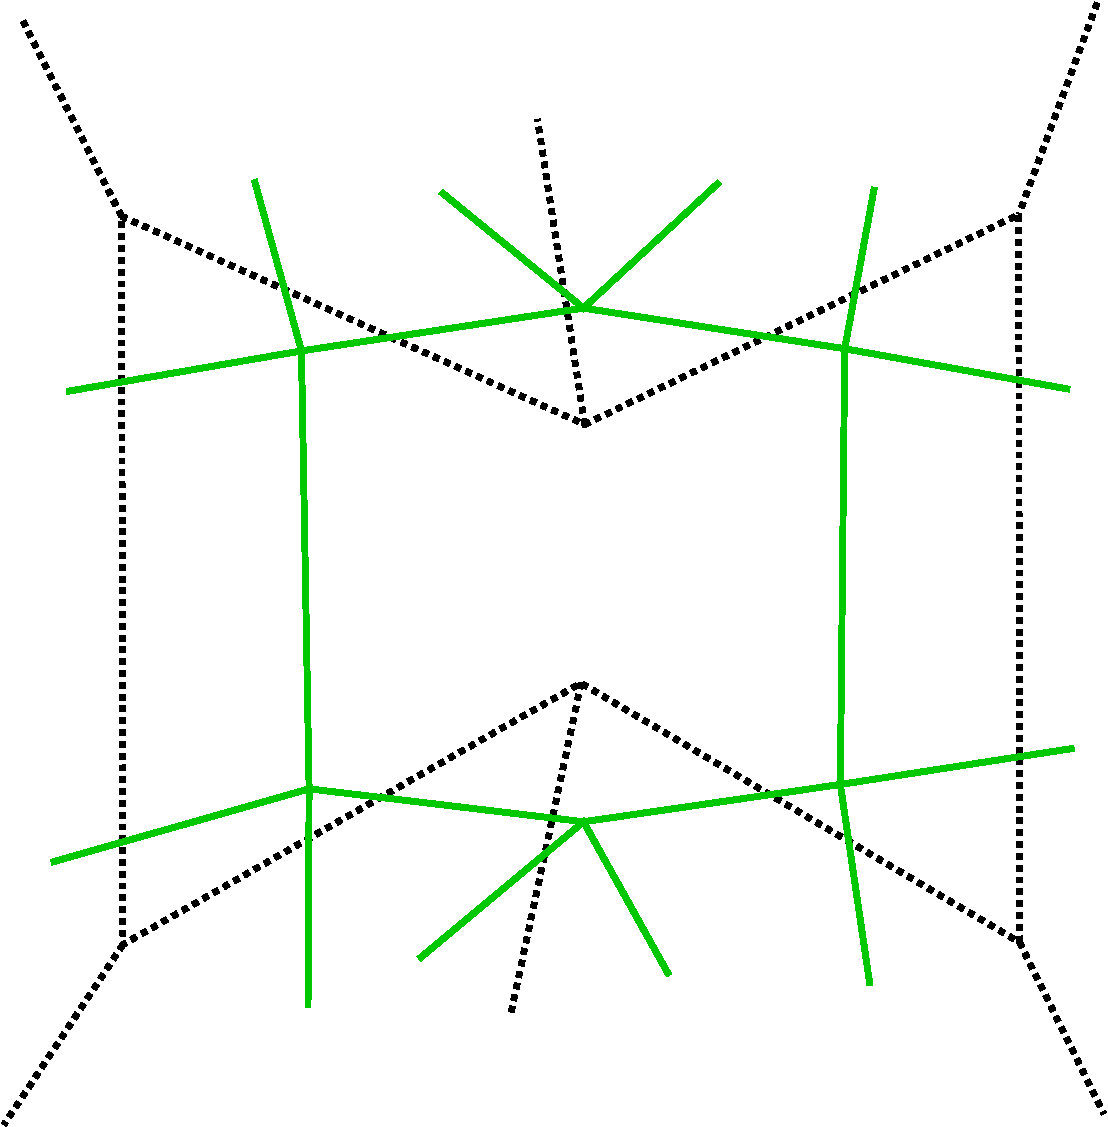
\includegraphics[scale=0.25]{doo_sabin_subdivision_example_2_crop}
	\quad
	\quad
	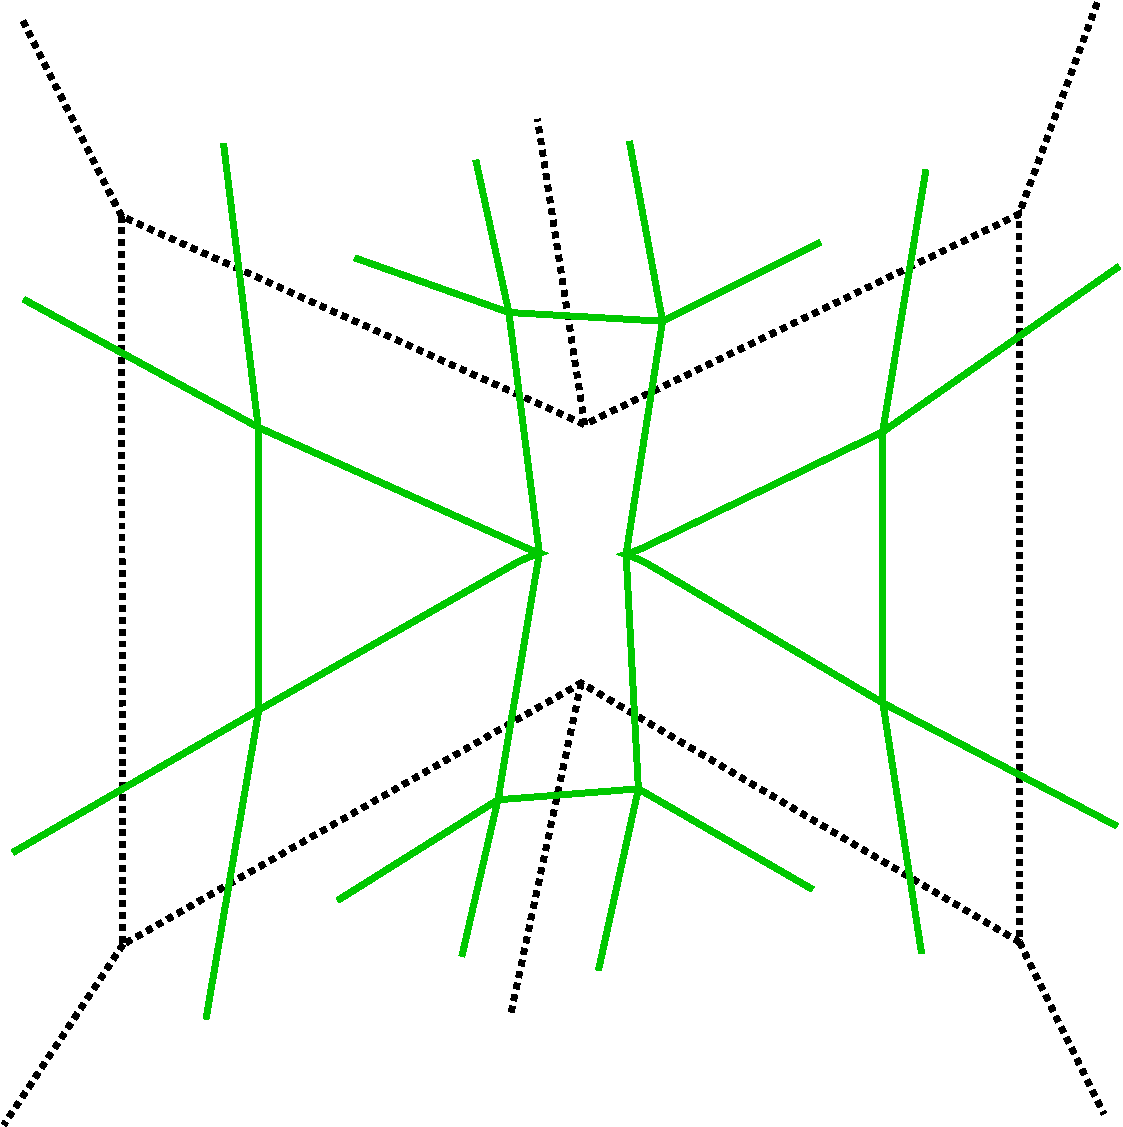
\includegraphics[scale=0.25]{euler_transformation_example_2_topological_changes_crop}
	\caption{\label{fig:exampdooeulertopochang} Doo-Sabin subdivision of a concave polygon (in dotted black) in input complex $K$ (left) and the Euler transformation of the same polygon with topological changes only (right).
        }
\end{figure}


%Our undirected graph($1$-skeleton of $\hat{K}$) is symmetric. Since graph is both edge transitive and vertex transitive implies symmetry. It is also $4$-regular, since every symmetric graph is regular. If we allow combinatorial changes then some of the vertices will have degree $6$ due to local Euler transformation. Hence even in worst case any vertex will be visited at most $3$ times.


\paragraph{Tool path}\label{sssec:toolpath}

While the perimeter and inset can typically be printed as continuous loops, tool path planning for printing the infill lattice commonly generates tool paths resembling a back and forth pattern, a spiral, or a fractal-like path for an arbitrary geometry.
The tool path consists of \textit{print paths} (material is pushed through the nozzle) and \textit{travel paths} (extruder moves from one location to other without pushing material).
Galceran and Carreras \cite{GaCa2013} described coverage path planning as assignment of finding a path that passes through all the points without obstacles.
Xu \cite{Xu2011} presented the use of graph-based algorithms in coverage problems.
General requirements for graph-based coverage problems such as all vertex coverage, non-overlapping and continuous paths, etc.~\cite{CaHuHa1988} are applicable in 3D printing as well, including the requirement that each edge should be printed.
One of the major steps in path planning is the identification of the tool path trajectory~\cite{DiPaCuLi2015}.
This tool path generation step involves filling interior regions and joining sub paths \cite{JiHeDu2017}.
While attempts have been made to join sub paths into a continuous path, they are all limited by increasing complexity of geometry.
Fewer sub paths in the tool path trajectory implies better quality of print.

Wang et al.~\cite{KuWuWa2019} developed $3$-dimensional infill (crossfill) using space filling curves, whose layer by layer cross-section is a continuous curve.
Crossfill curves are fit into the infill region by intersecting with boundary of the polygon in a given layer, but this step can create multiple components.
Later these components are connected into one continuous curve through an outer perimeter.
New edges added to create these components are not guaranteed to have a support below it.
We can still have material collision in each individual component if their boundary is too skewed or component is too thin (this is still an open problem; see Section \ref{sec:boundaryedges}). 
 
Use of graphical models in additive manufacturing was demonstrated recently by Dreifus et al.~\cite{Dretal2017}.
They mesh each layer of the print as a graph, and find an Eulerian cycle over all edges of the graph.
If the infill lattice is not Eulerian, they add "phantom edges" to the odd-degree vertices of the graph.
When the extruder reaches an odd degree vertex, it stops printing, lifts above the printed material, moves to its matched vertex, and resumes printing.
However, these stop and starts leave \textit{teardrops} of material in their wake, as the extruder drags excess material behind it.
Such teardrops weaken the print.
Also, stopping and starting repeatedly increases print times.
Further, their approach to identify the Eulerian cycle created \emph{crossovers} when pairs of sub-paths of the tour cross each other.

%\begin{comment}
%Add figures for all the defects we discussed delamination, saging, teardrop.
%\end{comment}

\section{Slicing}\label{sec:slicing}
The goal of our 3D printing approach is to have maximum continuous print path and minimum travel path (i.e., non-print path) in each layer.
Further, when printing multiple layers on top of each other, we want to ensure there is no printing in free space.
Ensuring we avoid printing in free space depends crucially on the geometric complexity of the object as well as on the first round of slicing.
We first formalize the condition that the sequence of layers generated by slicing must satisfy in order to prevent printing in free space (Section \ref{subsec:contilayers}).
We assume this condition is satisfied by the layers of the input to our \emph{clipping} procedure, which produces meshes for each polygon in a layer that are guaranteed to be Euler (Section \ref{subsec:clipping}).
 
%\input{Journal_epscont}
\subsection{$\epsilon$-Continuous Layers}\label{subsec:contilayers}
Let $\Ps_i = \{P_{ij}\}$ and $\Ps_{i+1} = \{P_{i+1,j}\}$ are sets of the polygons in two consecutive layers created by slicing.
The two layers are said to be $\epsilon$-continuous if for every point $\vx \in P_{i+1,j}$ there exists a point $\vy$ in \emph{some} $P_{ij} \in \Ps_i$ such that $ d(\vx, \vy) \leq \epsilon$ for \emph{all} $P_{i+1,j} \in \Ps_{i+1}$, where  $\epsilon = c r$ with $0 \leq c \leq 1$ and $r$ being the radius of extruder. % (see Figure \ref{fig:epsiloncontinuous}).
The parameter $c$ determines the maximum \emph{overhang} allowed for the material deposited in a layer over the material in the layer immediately below.
We assume there are sufficient numbers of perimeters in each layer to support the boundary edges in the layer above.
%Assuming the numbers of perimeters in the two layers are same, if two consecutive layers are not $\epsilon$-continuous then the print may collapse due to printing in free space.
%While one may be able to use varying numbers of perimeters in consecutive layers to avoid printing over free space in certain settings,
Value of $c$ is chosen based on various design and material considerations.
We assume the output of the slicing step in the design process produces layers that are $\epsilon$-continuous in consecutive pairs.

%\input{Journal_clip}
\subsection{Clipping}\label{subsec:clipping}
Suppose $\hK$ is the Euler transformation of $K$, which meshes the union of polygons $\displaystyle \cup_i \Ps_i = \cup_{i,j} P_{ij}$ from all layers, where $P_{ij} \in \Ps_i$ is the $j$th polygon in $i$th layer.
Each polygon $P_{ij}$ has a region $R_{ij}$ to be filled with infill lattice (note that $R_{ij} \subset P_{ij}$ can happen as some polygons may have edges along the boundary of the print domain).
Suppose $\tR_{ij}$ is the inward Minkowski offset with a ball of radius $r$, the extruder radius, of the region $R_{ij}$.
We will use $\tR_{ij}$ instead of $R_{ij}$ to generate the infill lattice for $P_{ij}$.
The reason behind this step is explained in Step \ref{itm:support} (to print the Support Perimeter).
Let polygons $R_{ij}$ and $\tR_{ij}$ be represented by the clockwise-ordered sequence of vertices $\{v_1, .... , v_n\}$ and $\{\tv_1, \dots , \tv_n\}$, respectively.
We define the \emph{clip} operation for intersecting (or clipping) a $2$-complex with a polygon, which may produce a $2$-complex that may have multiple components, and may not be pure.
We also define the \emph{patch} operation that converts the $2$-complex produced by a clip operation back into a connected pure $2$-complex.
%Let clipping $\hK$ with region $R_{ij}$ produce the $2$-complex $\tK$.
%Then $\tK$ consists of $2$-cells in $K$ interior to $R_{ij}$ and free edges formed by trimming those $2$-cells in $K$ which intersect $R_{ij}$.
%$\tK$ is not guaranteed to be a pure $2$-complex, since free edges do not belongs to any $2$-cells.
%The $1$-skeleton of $\tK$ is guaranteed to have an \textit{even} number of \textit{free edges}.
%This result follows from the handshake lemma that says an undirected graph has even number of odd-degree vertices.
%Since $\hK$ is Euler, only the vertices at the ends of free edges in $\tK$ have odd degree (of $1$ each).
%Hence there must be an even number of free edges.


\begin{defn} \label{def:clip}
  \emph{({\bfseries Clip})}
  We define how to construct $\tK$, the output of clipping the $2$-complex $\hK$ with polygon $\tR_{ij}$.
  %Anything contained in $\tR_{ij}$ is may be at the boundary or interior to $\tR_{ij}$.
  Add  to $\tK$ the polygons, edges, and vertices of $\hK$ contained in $\tR_{ij}$.
  For edges in $\hK$ cut by the boundary of $\tR_{ij}$, add to $\tK$ the portions inside $\tR_{ij}$ as new edges, and their points of intersection on the boundary of $\tR_{ij}$ as new vertices.
\end{defn}
%
Note that the result of a clip operation may not necessarily be a pure $2$-complex, and can have multiple components (see \cref{fig:multicomponent}).

\begin{defn} \label{def:patch}
  \emph{({\bfseries Patch})}
  Let $\tK$ be the output of a clip operation as specified in \cref{def:clip}.
  Suppose $S= \{\tv_{n+1}, \tv_{n+2}, .... , \tv_{n+m}\}$ is a clockwise ordered sequence of all points of intersection of $\tR_{ij}$ and the $1$-skeleton of $\hK$ with odd degrees in the $1$-skeleton of $\tK$
  (note that $m$ will be even).
  Since $\tR_{ij}$ can intersect edges in $\hK$ between or at their end point(s), vertices in $S$ can be terminal or boundary vertices in the $1$-skeleton of $\tK$.
  Join alternate pair of vertices in $S$ by a clockwise path on $\tR_{ij}$ as shown in Figure \ref{fig:printingprocess}.
  There are two possible choices of joining alternate pairs of vertices ($1$-$2$, $3$-$4,\dots$ or $2$-$3$, $4$-$5,\dots$).
  Pick the option that ensures the end vertices of components represented by subsequences of $S$ are connected by these paths to end vertices of adjacent components.
  Also add new polygons to $\tK$ whose edges include the edges in new paths added as described above, new edges added by the clip operation on $\hK$, and the edges of $\hK$ contained in $\tR_{ij}$.	
\end{defn}

We show that the patch operation restores the Euler and connected nature of the input complex.

\begin{lem}\label{lem:singlecomponent}
  If $\hK$ is a connected pure $2$-complex and its $1$-skeleton is Euler, then $\tK$ produced by the patch operation on $\hK$ is a connected pure $2$-complex and its $1$-skeleton is Euler. 
\end{lem}
\begin{proof}
  Clipping $\hK$ with region $\tR_{ij}$ can create multiple components in the infill lattice if $\tR_{ij}$ intersects any polygon in $\hK$ more than two times, or an edge more than once, or all edges connected to a vertex (see \cref{fig:multicomponent}).
  Each component created in this process has an even number of odd degree vertices (by handshake lemma).

  Let $S' =\{\tv_1, \dots, \tv_p\}$ be a clockwise ordered subsequence of vertices in $S$ of some component (with $p < m$).
  As specified in \cref{def:patch}, we join alternate pairs of vertices in $S'$ by a path on $R_{ij}$ (also see the Clipping Step \ref{itm:patch}) such that edge $\{\tv_1, \tv_2\}$ is not included.
  Since $p$ is even, edge $\{\tv_{p-1}, \tv_{p}\}$ is also not included.
  Hence the first and last vertices in $S'$ ($\tv_1$ and $\tv_p$) are left unpaired, but all intermediate vertices are now connected to $\tK$.
  In this case, the patch operations (in the Clipping step) will necessarily pair $\tv_1$ with a similar unpaired end vertex of the previous component, and also pair $\tv_p$ with the unpaired start vertex of the next component.
  Hence the extra edges added by the patch steps ensure that we get a single connected component.
  Also note that each odd degree vertex gets one additional edge, thus making its degree even.
  Hence the $1$-skeleton of $\tK$ is Euler.
  Finally, the new polygons added to $\tK$ (as specified at the end of \cref{def:patch}) ensure that the resulting complex is pure.
\end{proof}
\vspace*{-0.15in}

\begin{figure}[ht!]
  \centering
  \begin{subfigure}[t]{2in}
    \centering
    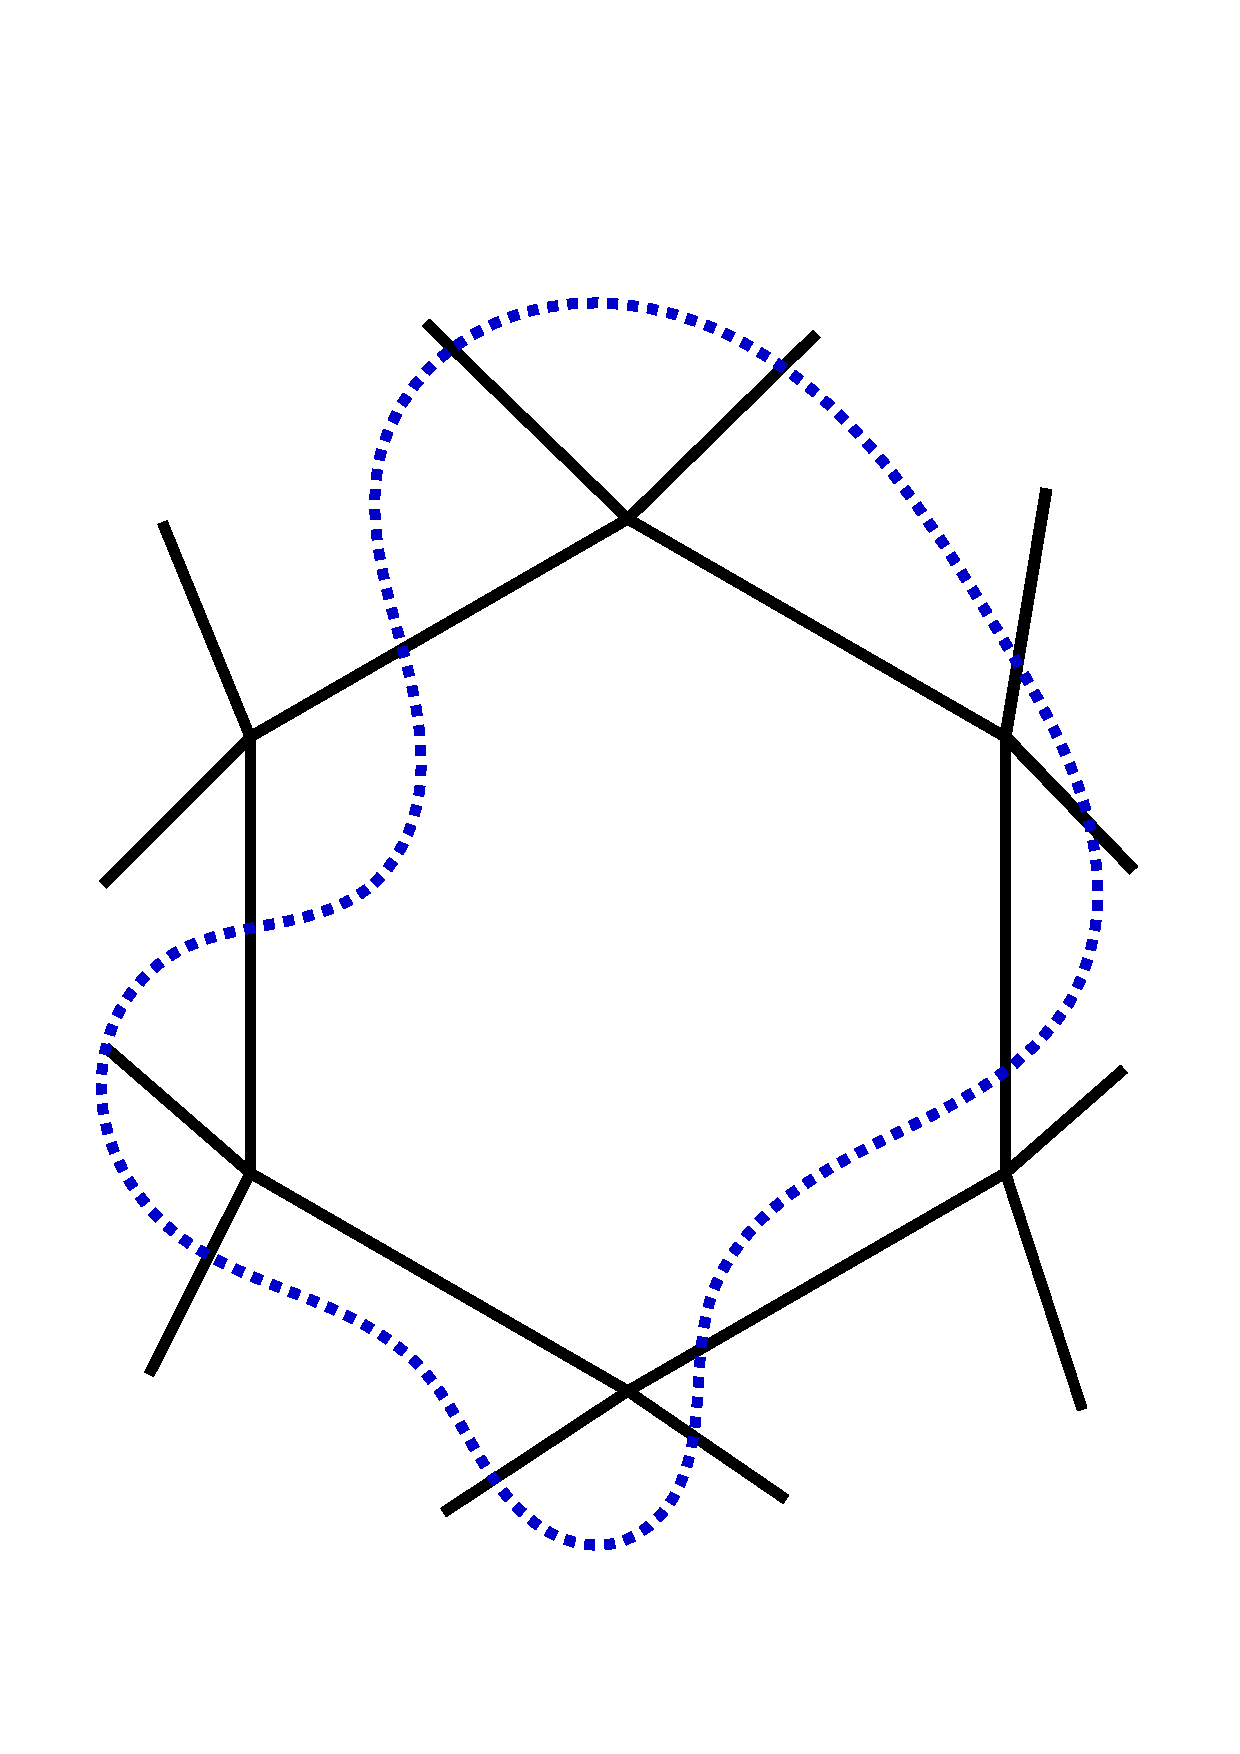
\includegraphics[scale=0.20]{multi_component_fig_1_crop}
    \caption{\label{fig:multicomponenta}}
  \end{subfigure}
  \begin{subfigure}[t]{2in}
    \centering
    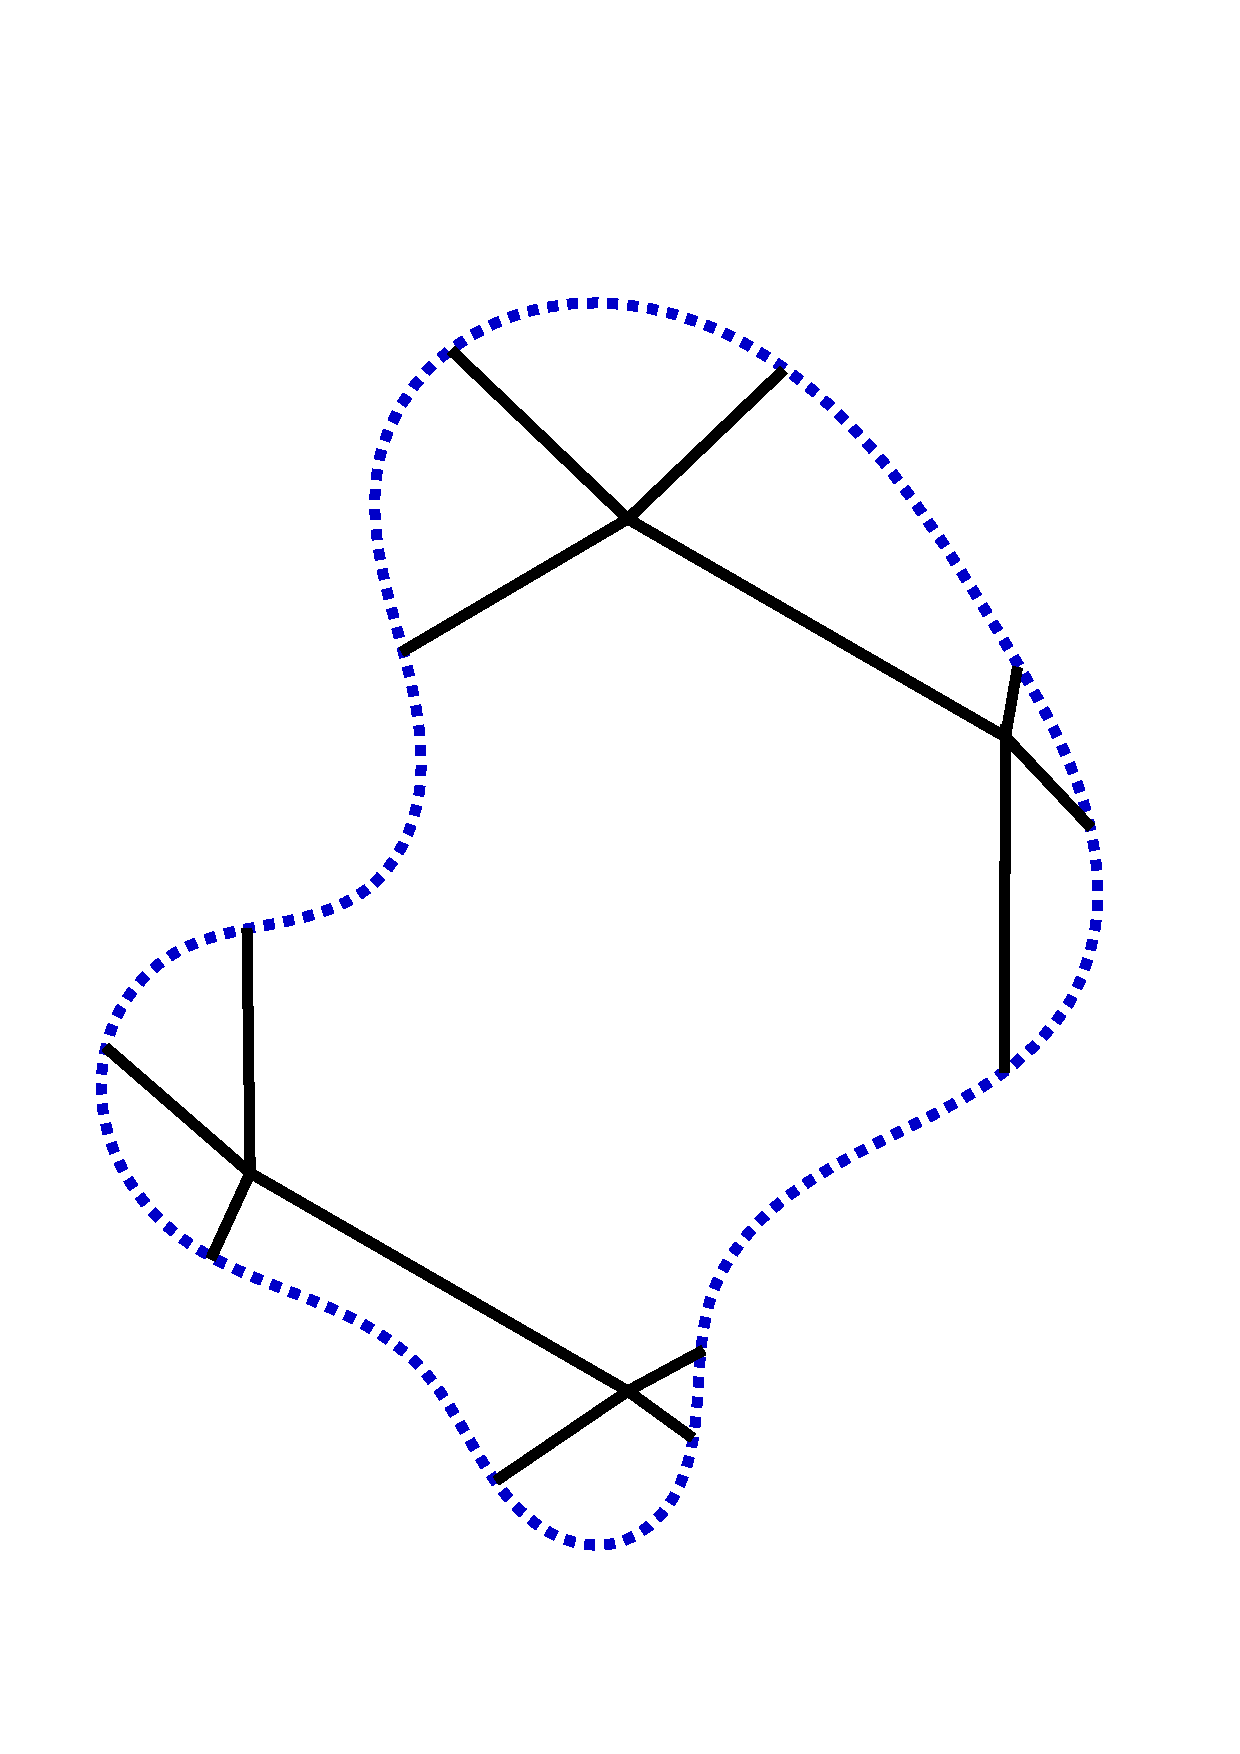
\includegraphics[scale=0.20]{multi_component_fig_2_crop}
    \caption{\label{fig:multicomponentb}}
  \end{subfigure}
  \begin{subfigure}[t]{2in}
    \centering
    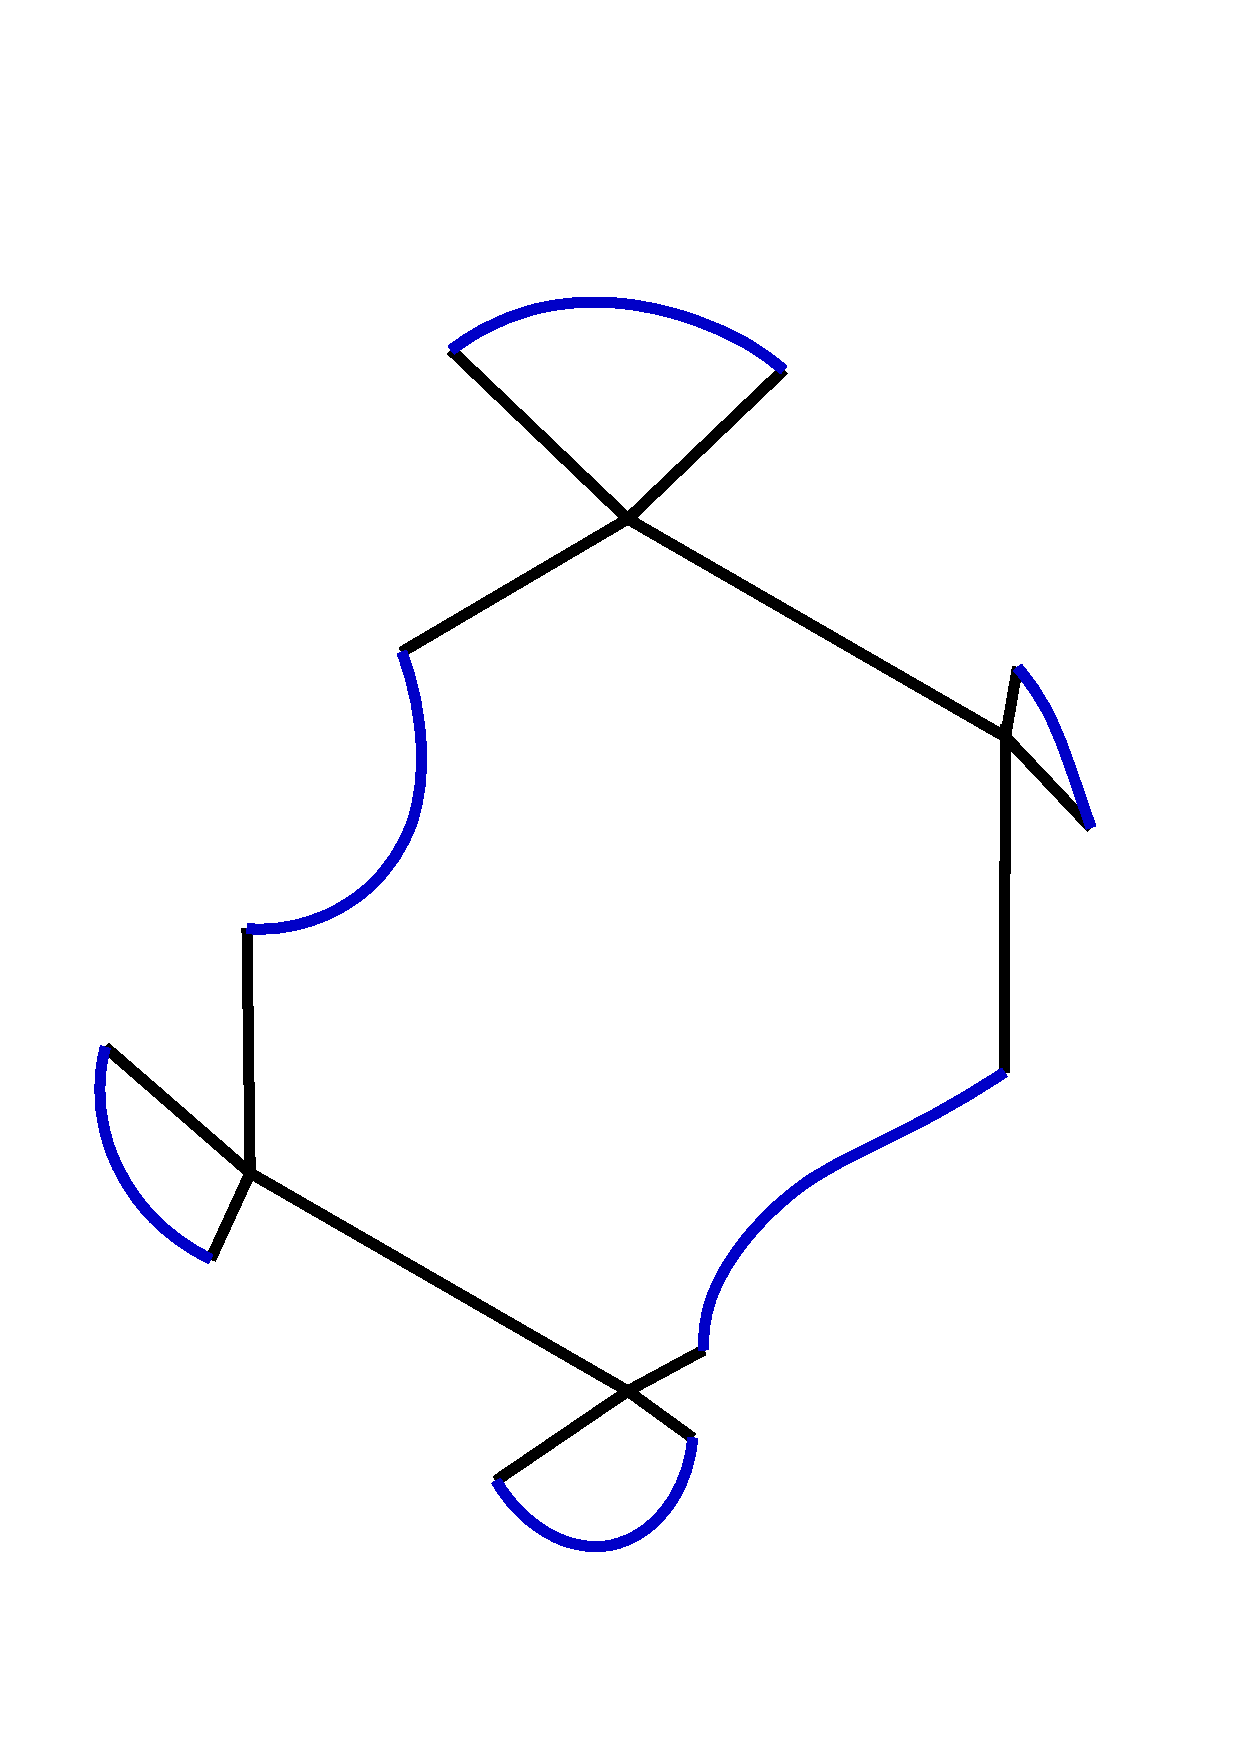
\includegraphics[scale=0.20]{multi_component_fig_5_crop}
    \caption{\label{fig:multicomponentc}}
  \end{subfigure}
  %\hspace*{.5in}
  \begin{subfigure}[t]{2in}
    \centering
    \includegraphics[scale=0.20]{multi_component_fig_3_crop}
    \caption{\label{fig:multicomponentd}}
  \end{subfigure}
  \begin{subfigure}[t]{2in}
    \centering
    \includegraphics[scale=0.20]{multi_component_fig_4_crop}
    \caption{\label{fig:multicomponente}}
  \end{subfigure}
  %\hspace*{.5in}
  \begin{subfigure}[t]{2in}
    \centering
    \includegraphics[scale=0.20]{multi_component_fig_6_crop}
    \caption{\label{fig:multicomponentf}}
  \end{subfigure}

  \caption{\label{fig:multicomponent}
    (a),(d) show one $2$-cell(Black) of complex $\hK$. Figure (b), (e) shows multiple components after \ref{def:clip} clip operation on $\hK$ with respective polygon(Dotted Blue) in some layer on Figure (a), (d). Figure (c), (f) shows \ref{def:patch} patch operation on Figure (b), (e) connecting multiple components with Solid Blue lines.}
\end{figure}

\begin{figure}[htp!] 
  \centering
  \begin{subfigure}[t]{1.6in}
    \centering
    \includegraphics[scale=0.15]{infill_pattern_input_complex_scheme}
    \caption{\label{fig:printingprocessa}}
  \end{subfigure}
  \hspace*{0.3in}
  \begin{subfigure}[t]{1.6in}
    \centering
    \includegraphics[scale=0.15]{infill_pattern_transformed_complex_scheme}
    \caption{\label{fig:printingprocessb}}
  \end{subfigure}	
  \begin{subfigure}[t]{1.6in}
    \centering
    \includegraphics[scale=0.22]{infill_pattern_transformed_complex_cookie_cut_fig_8_crop}
    \caption{\label{fig:printingprocessc}}
  \end{subfigure}
  
  \caption{\label{fig:printingprocess}
    (a) Projected polygon $P$(purple) and initial $2$-complex K is in black. (b) Euler transformation $2$-complex $\hK$(green), Region $\tR_{ij}$(red dot) of some polygon $P_{ij}$. (c) $\hK$ is clipped using $\tR_{ij}$ and patched to $2$-complex $\tK$(green) after step \ref{itm:patch}, where $\tR_{ij}$ has  $\{\tv_1, \dots , \tv_{24}\}$ sequence of vertices and $\{\tv_{25}, ..... , \tv_{36}\}$ are points of intersection of $\tR_{ij}$ and $1$-skeleton of $\hK$.
  }
\end{figure}

\vspace*{-0.05in}
\subsection{Continuous Tool Path Planning Framework: Steps} \label{ssec:steps}
\vspace*{-0.05in}

Our framework for continuous tool path planning consists of the following steps.
\begin{enumerate}
  \item {\bf{\textit{Slicing:}}}
    Slice an STL file of the design.
    This step creates a sequence of layers, and each layer can have multiple polygons.
    Let $\Ps_i = \{P_{ij}\}$ be the set of all the polygons in layer $i$ with or without holes.
    We assume the layers generated by slicing are $\epsilon$-continuous.
    
  \item{\bf{\textit{Projecting:}}}
    Project all polygons $\{P_{ij}\}$ in each layer $\Ps_i$ on to the horizontal plane.
    Take the {\bfseries union} of all projected polygons (from all layers).
    This union can have an irregular shape depending on the input.
    %Also, the projection set could affect quality parameter of input complex $K$.
    Let $P$ be the convex hull of the union of projected polygons.
    Note that taking the convex hull will avoid irregularities.
    We are assuming the input design has a single component.
    If not, we can repeat the procedure for each component.

  \item{\bf{\textit{Meshing:}}}
    Mesh $P$ with a pure $2$-complex $K$.
    We assume $K$ satisfies \cref{asmn:Kholesoutside}.
    
  \item \label{itm:eulertransform}{\bf{\textit{Euler Transformation:}}}
    Apply Euler Transformation to $K$ to create $\hK$.
    We assume that the traversal of edges in $\hK$ will not be affected by extruder size considerations (see \cref{sec:boundaryedges}).
    
  \item\label{itm:patch}{\bf{\textit{Clipping:}}} 
    $\tK$ is a $2$-complex contained in $\tR_{ij}$.
    It is generated by clip (\cref{def:clip}) and patch (\cref{def:patch}) operations on $\hK$ with respect to $\tR_{ij}$ as illustrated in \cref{fig:printingprocess}.
    By \cref{lem:singlecomponent}, we get that $\tK$ is connected and its $1$-skeleton is Euler since $\hK$ has a single component and its $1$-skeleton is Euler. 
    There are two possible choices of pairing alternate vertices for patch operation.
    We can choose arbitrarily between them as long as $\tK$ is a single component. 
    
    Printing the infill lattice in each layer amounts to printing edges in the $1$-skeleton of $\tK$.
    We clip the $2$-subcomplex $\tK$ for each layer from $\hK$ to prevent printing in free space.
    Each edge is supported by an edge in the layer below it except for boundary edges in $\tK$.
    We will add a support perimeter to support boundary edges in $\tK$, as discussed in the next step. 
      
  \item\label{itm:support}
    {\bf{\textit{Support Perimeter:}}}
    Let $\tR_{ij} \in P_{ij}$ and $\tR_{i+1,j} \in P_{i+1,j}$ be such that $\tR_{i+1,j}$ is supported by $\tR_{ij}$ through $\epsilon$-continuity as shown in \cref{fig:step_6_reasoning}.
    There are two possible ways we can select alternate pairs of vertices for subcomplex $\tK$ to join in $\tR_{i+1,j}$: $\{\{12, 13\}, \{14, 15\}, \{16, 11\}\}$ or $\{\{11, 12\}, \{13, 14\}, \{15, 16\}\}$. % (see \cref{fig:step_6_reasoning}).
    Then the edges $\{12, 13\}$ in the first case and $ \{11, 12\}, \{13, 14\}$ in second case are not supported if $\{2, 3\},\{4, 5\}, \{6, 7\}, \{8, 9\},$ and $\{10, 1\}$ are the vertices pairs selected for $\tR_{i+1,j}$.
    To solve this problem we need a way to print all the edges at boundary of the polygons.
    \begin{figure}[htp!] 
  	\centering
  	\includegraphics[width=50mm,height=50mm]{step_6_reasoning-crop}
  	\caption{\label{fig:step_6_reasoning}
          $\tR_{ij}$ (blue) in $P_i$, $\tR_{i+1j}$ (blue) in $P_{i + 1}$ intersect the complex $\hK$ (green) at points $\{1, \dots,10\}$ and $\{11, \dots, 16\}$, respectively.
        }
    \end{figure}  
  
    Since we are not printing all the edges at the boundary of $\tR_{ij}$, we could have some overhanging boundary edges in $\tK$.
    Let $\tP$ be the nonprinted path on $\tR_{ij}$ between $\tv_{n + l}$ and  $\tv_{n+l+1}$, which are vertices of $S$ on $\tR_{ij}$.
    Add circles of radius $r$, the extruder radius, on $\tv_{n+l}$ and $\tv_{n+l+1}$ and on path $\tP$ such that neighboring circles do not intersect.
    We assume the circles only intersect neighboring line segments on the path.
    Suppose $\eta$ is the maximum number of circles of radius $r$ that can be added on path $\tP$, assuming there are $2$ circles of radius $r$ centered at end points of the path.
    Add $\eta$ possible circles on path $\tP$, where the center of the $j^{\mbox{th}}$ circle is $\tv'_j$.
    The total gap we can have between the circles is $2r - \delta$, where $0 < \delta < 2r$ as shown in \cref{fig:supporta}.
    We can uniformly distribute the gap of $(2r - \delta)/(\eta + 1)$ between the circles as shown in \cref{fig:supportb} assuming $\eta$ is at least one.
    Since $\tR_{ij}$ is the inward Minkowski offset of $R_{ij}$ with a $2$-ball of radius $r$, for any $\tv'_j$ there exists a point $a$ such that line segment $\{\tv'_j, a\}$ is perpendicular to $\tR_{ij}$ and $R_{ij}$, and  $d(\tv'_j, a) = 2r$.
    Let $v_{n+k}$ and $v_{n+k+1}$ be points of intersection with $R_{ij}$ of the circle of radius $r$ centered at $a$.
    Create a corner by adding edges $\{v_{n+k}, a\}$, $\{v_{n +k +1}, a\}$ as shown in Figure \ref{fig:supportc}.
    Connect end points of the corners by a path on $R_{ij}$ if corner line segments do not intersect each other.
    Else change end points to the points of intersection so as to form a simple closed polygon as shown in \cref{fig:supportd}.
    We illustrate in \cref{fig:supportperimeter} the support perimeter around $\tK$ shown in \cref{fig:printingprocessc}.
    
 \begin{figure}[htp!]    
   %\hspace*{-0.8in}
   \begin{subfigure}[t]{3in}
     \centering
     \includegraphics[scale=0.30]{support_fig_1_crop}
     \vspace*{-0.25in}
     \caption{\label{fig:supporta}}
   \end{subfigure}
   \begin{subfigure}[t]{3in}
     \centering
     \includegraphics[scale=0.30]{support_fig_2_crop}
     \vspace*{-0.25in}
     \caption{\label{fig:supportb}}
   \end{subfigure}
 
   \begin{subfigure}[t]{3in}
     \centering
     \includegraphics[scale=0.30]{support_fig_3_crop}
     \vspace*{-0.25in}
     \caption{\label{fig:supportc}}
   \end{subfigure}	
   \begin{subfigure}[t]{3in}
     \centering
     \includegraphics[scale=0.30]{support_fig_4_crop}
     \vspace*{-0.25in}
     \caption{\label{fig:supportd}}
   \end{subfigure}
   \caption{\label{fig:support}
     (a) Portion of $R_{ij}$ (blue) and $\tR_{ij}$ (red), $\tP$ (red), with total gap between circles being $2r - \delta$.
     (b) Uniformly distribute the gap between neighboring circles $\frac{2r - \delta}{9}$.
     (c) $\{v'_j, a\}$ is perpendicular to $\tR_{ij}$ and $R_{ij}$, circle centered at $a$ intersects $R_{ij}$ at $v_{n+k}, v_{n+k+1}$, and corner (pink) after adding edges $\{v'_j, v_{n+k}\}, \{v'_j, v_{n + k + 1}\}$.
     (d) Neighboring corners joined (pink) to form simple closed polygon.
     }
 \end{figure}    

 \begin{figure}[htp!] 
   \centering
   \vfill
   \includegraphics[scale=0.30]{infill_pattern_transformed_complex_cookie_cut_support_crop}
   \caption{Support perimeter for $\tK$ shown in \cref{fig:printingprocessc} is shown in blue here. }
   \label{fig:supportperimeter}
 \end{figure}   	 
\end{enumerate}


%\bigskip

\begin{rem}
  {\rm 
  In Step \ref{itm:support} above, we add corners only if we can add circles of radius $r$ on path $\tP$, given there are circles of radius $r$ at the end point of the path.
  It is not guaranteed that line segments of $\tP$ will be covered by the support, since the coverage depends on the curvature of $\tP$ as shown in Figure \ref{fig:supportd}.
  An alternative approach to printing the support is to print the individual non-printed sections in $\tR_{ij}$ while making non-print travel moves in between.
  But this approach will have $m/2$ starts and stops.
  If $\hK$ is a highly dense $2$-complex, then $m$ will be large and we will have a large number of starts and stops in this case.
  }
\end{rem}

\begin{rem}
  {\rm
    A continuous tool path exists only if any polygon in $\tK$ is shrinkable (\cref{def:shrinkable}) with no topological changes.
    But boundary polygons in $\tK$ due to clip and patch (\cref{def:clip,def:patch}) operations can be shrinkable with topological changes or unshrinkable as mentioned in \cref{sec:boundaryedges}.
  }
\end{rem}

\section{Generalized Euler Transformation} \label{sssec:genET}
We now consider generalizations of the Euler transformation where we could relax some of the assumptions we make on the input complex (\cref{asmn:Kholesoutside}).
We eventually want to allow combinatorial and topological changes in the polygons undergoing transformation.

Consider a $2$-complex $K$ consisting of a single polygon $f$.
$K$ does not satisfy the input condition for Euler transformation, since adjacent edges are shared with the outside (Figure \ref{fig:2cellpartition}).
Nevertheless, we apply the transformation to $K$.
In the resulting $\hK$, all vertices will have odd degree (circled in Figure \ref{fig:2cellpartition}).
But this $\hK$ satisfies the input condition, since any pair of adjacent edges of a polygon in $K$ now belong to two new polygons in $\hK$.
Hence if we apply the Euler transformation again to $\hK$, i.e., we apply it \emph{twice} on $K$, the resulting complex has a $1$-skeleton that is Euler in the default setting (without combinatorial and topological changes in class-$1$ polygons), even if adjacent edges of a polygon in $K$ are boundary edges.
More generally, we define this process as the generalized Euler transformation.

\begin{defn}
	\label{def:genET}
	(Generalized Euler Transformation in $d=2$)
	Let $K$ be a $2$-dimensional cell complex in $\R^2$ with polygons possibly having adjacent boundary edges.
	Apply the Euler transformation on $K$ to obtain $\hK$, even if $K$ do not satisfy input conditions \ref{asmn:Kholesoutside}.
	$\hK$ will always satisfy \cref{asmn:Kholesoutside}, so now apply Euler transformation on $\hK$.
\end{defn}
We could use the generalized Euler transformation to improve mechanical properties of the design (by increasing the density of the mesh) in some regions while still guaranteeing that the $1$-skeleton of the $2$-complex is Euler.
Notice that the density of the mesh is increased by this process, as shown in following result. 
\begin{lem}
  \label{lem:trgrrate} 
  After $m$ rounds of transformation of input complex $K$, the number of vertices $|\hat{V}^m| = 2\cdot 4^{m-1}|E|$ and number of edges $|\hat{E}^m|=4^m|E|$.	
\end{lem}
\begin{proof}
  After the first transformation, we get $|\hat{E}^{1}| = 4 |E|$ (by \cref{lem:cntshVhEhF2d}).
  And after the second transformation we get $|\hat{E}^2| = 4 |\hat{E}^1| = 4^2|E|$.
  Extending the argument, after $m$ transformations we get $|\hat{E}^m| = 4^m |E|$.
  Similarly, we get $|\hat{V}^1| = 2 |E|$, then $|\hat{V}^m| = 2 |\hat{E}^{m-1}| = 2\cdot4^{m-1}|E|$.     	
\end{proof}
The above result shows that the numbers of vertices and edges grow significantly after each iteration of transformation.
Hence the generalized Euler transformation may create a large number of edges.

We now discuss Euler transformation with \emph{combinatorial} and \emph{topological} changes to a polygon resulting from its mitered offset. 

\subsection{Euler Transformation with Combinatorial changes}\label{sec:eulertransformwithcombin}

Suppose $\hf, \hf_e, \hf_v$ are $3$ classes of polygons corresponding to a polygon ($f$), edge ($e$), and a vertex($v$) in $K$.
Maximum mitered offset in a polygon of the input complex $K$ is limited by the smallest edge length, as the mitered offset in our original Euler transformation assumes no combinatorial and topological changes in $\hf$.
\textit{Combinatorial change in $\hat{K}$ is a change in number of edges of some class-$1$ polygon $\hat{f}$ in $\hat{K}$ from corresponding polygon in $f$ in $K$.} 
Suppose polygon $f$ has $n$ edges and is now permitted to have combinatorial changes when generating its mitered offset.
Then we can reduce at most $n-3$ edges as we want $\hf$ to still be a polygon, and a polygon has at least $3$ edges.
If $\hf_e$ is sharing edges with two Class $1$ polygons and if both of those edges are reduced, then $\hf_e$ will collapse into an edge as shown in Figure \ref{fig:eulertransfecollapse}.
Since Class $3$ polygons ($\hf_v$) do not share edges with any Class $1$ polygons, combinatorial changes in the Euler transformation will not affect the number of edges in $\hf_v$.
%
\begin{figure}[ht!] 
  \centering
  \includegraphics[scale=0.20]{input_complex_combinatorial_change_class_2_cell_collapse_fig_1_crop}
  \quad
  \includegraphics[scale=0.25]{intermediate_complex_combinatorial_change_class_2_cell_collapse_fig_1_crop}
  \quad
  \includegraphics[scale=0.25]{output_complex_combinatorial_change_class_2_cell_collapse_fig_1_crop}
  \caption{\label{fig:eulertransfecollapse}
    Two polygons of a $2$-complex $K$ in the plane (top).
    Euler transformation of $K$ into $\hK$ (middle), where $\hf, \hf'$ are Class $1$ polygons and $\hf_e$ (red) is a Class $2$ polygon corresponding to edge $e$ (red) in $K$.
    Class $2$ polygon $\hf_e$ is collapsed to an edge $\he$ and red circled vertices have odd degree (bottom).
  }
\end{figure}

\begin{figure}[htp!] 
	\centering
	\includegraphics[scale=0.25]{lemma_edge_contraction_fig_1_crop}
	\hspace*{0.4in}
	\includegraphics[scale=0.35]{lemma_edge_contraction_fig_2_crop}
        \vspace*{0.1in}\\
	\includegraphics[scale=0.35]{lemma_edge_contraction_fig_3_crop}
	\hspace*{0.4in}
	\includegraphics[scale=0.35]{lemma_edge_contraction_fig_4_crop}
	\caption{\label{fig:lemmaedgecontraction}
		$f$ is a polygon in $K$ (top left).
		Euler transformation of $K$ into $\hK$ (top right), where $\hf$ is the Class $1$ polygon corresponding to $f$, and $\hf_e$ (blue) is the Class $2$ polygon corresponding to edge $e$.
		Combinatorial changes are allowed in $\hK$ in the bottom left figure, and edge $\he$ of $\hf$ is collapsed to a point $\hv$ where $\hf_e$ (blue) is a triangle.
		As $\he \in \hf_e$ is collapsed to a point, the degree of $\hv$ in the $1$-skeleton of $\hK$ is $2(2) + 4 = 8$.
		In the version of $\hK$ shown in the bottom right figure, an edge of $\hf_e$ shared with some Class $1$ polygon other than $\hf$ is also collapsed to a point.
		Here, $\hf_e$ is collapsed to an edge $\he'$ (red) and the degree of $\hv$ in the $1$-skeleton of $\hK$ is $2(2) + 4 - 1= 7$.
	}
\end{figure}

\begin{figure}[hbp!] 
  \centering
  \includegraphics[scale=0.3]{2_cell_partition_fig_1_crop}
  \hspace*{0.25in}
  \includegraphics[scale=0.3]{2_cell_partition_fig_2_crop}
  \hspace*{0.25in}
  \includegraphics[scale=0.3]{2_cell_partition_fig_3_crop}
  \caption{\label{fig:2cellpartition}
    $\hK$ consisting of a single polygon $f$ (left) and its Euler transformation $\hK$ in green (middle).
    Vertices circled in red have odd degrees.
    The complex in blue (right) is the Euler transformation of $\hK$, and its $1$-skeleton is Euler.}
\end{figure}

\begin{lem}
  \label{lem:combinatorialdegree}
  Let $\hv$ is a vertex in a Class $1$ polygon $\hf$ of $\hK$ created after collapsing $\pi$ adjacent edges in $\hf$, where $\hf$ is allowed to have combinatorial changes.
  Let $\hf_e$ is some Class $2$ polygon that contains one of these collapsed adjacent edges.
  If no $\hf_e$ is collapsed into an edge, then degree of $\hv$ is $~2\pi + 4~$ else $~2\pi + 4 - m~$ where $m$ is the number of polygons similar to $\hf_e$ collapsed into an edge. 
\end{lem}
\begin{proof}
  Since a polygon $\hf$ is allowed to have combinatorial changes in $\hK$, it will change degree of vertices in $\hf$.
  $\pi$ adjacent edges in $\hf$ have $\pi + 1$ vertices.
  Each end vertex of the path created by $\pi$ adjacent edges adds $3$ edges to $\hv$, and each interior vertex of the path adds $2$ edges to $\hv$ as shown in \cref{fig:lemmaedgecontraction}.
  This implies $\hv$ has degree $2(\pi -1) + 3 + 3 = 2\pi + 4$ and $1$-skeleton of $\hK$ is still Euler.
  If $m > 0$ Class $2$ polygons sharing one of these adjacent edges are allowed to collapse into an edge, then $2$ edges sharing $\hv$ of each collapsed Class $2$ polygon is replaced by one edge.
  Also, $m \leq \pi$ since each distinct edge in any Class $1$ polygon is shared by a unique Class $2$ polygon in the Euler transformation.
  This implies $\hv$ has degree $2\pi + 4 -2m + m = 2\pi + 4 - m$ and $1$-skeleton of $\hK$ is Euler depending upon $m$ is even or odd, as shown in Figure \ref{fig:lemmaedgecontraction}.
\end{proof}
%\clearpage


If combinatorial changes are allowed during Euler transformation, then for any odd degree vertices created, we should apply Euler transformation to a local complex.
In the following result, we use the generalized Euler transformation to address the issue of odd degree vertices that may be created by combinatorial changes in $\hK$.
%\newline


\begin{lem}
  \label{lem:localeulertransformation}
  Suppose $\hf_e$ in $\hK$ is collapsed to an edge $\he$, since combinatorial changes are allowed in $\hK$.
  Suppose $\hk$ is a sub $2$-complex of $\hK$ consisting of Class $3$ polygons sharing any edge $\he$ in $\hK$,
  and let $\hk_j$ be a single component contained in $\hk$, since $\hk$ can have multiple components.
  Suppose $\hk_j = \cup \tilde{k}_i$, where $\tilde{k}_i$ is sub $2$-complex in $\hk_j, \hK$, and let $\tilde{k}_i, \tilde {k}_j$ do not share any edge in $\hK$, if $i \neq j$.
  If $\check{k}_i$ is the generalized Euler transformation of $\tilde{k}_i$ and $\bar{k}_j = \cup \check{k}_i$ is single component in $\bar{k}$, then the $1$-skeleton of $(\hK \smallsetminus \hk) \cup \bar{k}$ is Euler.  	
\end{lem}



\begin{figure}[htp!] 
  %\centering
  \begin{subfigure}[t]{2.5in}
    \centering
    \includegraphics[scale=0.38]{lemma_local_euler_transformation_fig_1_crop}
    \caption{\label{fig:lemmalocaleulertransformationa}}
  \end{subfigure}
  \hspace*{0.8in}
  \begin{subfigure}[t]{2.5in}
    \centering
    \includegraphics[scale=0.38]{lemma_local_euler_transformation_fig_2_crop}
    \caption{\label{fig:lemmalocaleulertransformationb}}
  \end{subfigure}
  \vspace*{0.3in}\\	
  \begin{subfigure}[t]{2.5in}
    \centering
    \includegraphics[scale=0.38]{lemma_local_euler_transformation_fig_3_crop}
    \caption{\label{fig:lemmalocaleulertransformationc}}
  \end{subfigure}
  \hspace*{0.8in}		
  \begin{subfigure}[t]{2.5in}
    \centering
    \includegraphics[scale=0.38]{lemma_local_euler_transformation_fig_4_crop}
    \caption{\label{fig:lemmalocaleulertransformationd}}
  \end{subfigure}
  \caption{  \label{fig:lemmalocaleulertransformation}
    (a) $f, f', f''$ are polygons in $2$-complex $K$.
    (b) $2$-complex $\hK$ after Euler transformation with combinatorial changes to some polygons in $\hK$. Class $2$ polygons $\hf_e,\hf_{e'}, \hf_{e''}$ corresponding to $e, e', e''$ in $K$ are collapsed into edges $\he, \he', \he''$.
    Sub $2$-complex $\tilde{k}_i$ (in blue) of some $\hk_j$ in $\hK$ consists of Class $3$ polygons sharing edges $\he, \he', \he''$ in the $1$-skeleton of $\tilde{k}_i$, and has vertices $\hv, \hv'$ with odd degree $7$.
    The number of edges (green) at each vertex of $\tilde{k}_i$ not in $\tilde{k}_i$ are even, $\hv$ has $1$ Class $3$ polygon(yellow) not contained in $\tilde{k}_i$. (c),(d) shows generalized Euler transformation of $\tilde{k}_i$. (d) $\check{k}_i$(blue) is generalized Euler transformation of $\tilde{k}_i$ and $\hv, \hv'$ including other vertices of $\check{k}_i$ has even degree in $1$-skeleton of $\hK \smallsetminus \tilde{k}_i \cup \check{k}_i$.
  }
\end{figure}

\begin{proof}
  Since combinatorial changes are allowed in $\hK$, let $\hv$ be a vertex in $\hk_j$ created after $\pi$ adjacent edges of $\hf$ are collapsed to a vertex.
  $\hk_j$ is single component in $\hk$, and only Class $3$ polygons share an edge with any collapsed Class $2$ polygons $\hf_e$ is in $\hk_j$.
  Hence $\hv$ can be shared by some Class $3$ polygon not in $\hk_j$.
  If any Class $3$ polygon sharing $\hv$ is not contained in $\hk_j$, this Class $3$ polygon does not share an edge with any Class $2$ polygon.
  Hence such cells do not belong to any component $\hk_j$ in $\hk$.
  Since Class $1$ polygons are edge disjoint from any Class $3$ polygons, and there are some Class $3$ polygons and $1$ Class $1$ polygon ($\hf$) sharing vertex $\hv$ in $\hK$ but not contained in $\hk_j$, we get that $\hv$ is shared by an even number of additional edges not in $\hk_j$.
  Since Class $1$ and Class $3$ polygons are edge disjoint in $\hK$, then any vertex($\hv'$) in some Class $3$ polygon in $\hk_j$ not similar to $\hv$ has $2$ more edges, not in $\hk_j$ sharing $\hv'$.
  Hence all the vertices in $\hk_j$ have even number of additional edges in $\hK$ not contained in $\hk_j$ as shown in Figure \ref{fig:lemmalocaleulertransformation}.
  
  Let $\check{k}_i$ be the generalized Euler transformation of each sub $2$-complex $\tilde{k}_i \in \hk_j$.
  Then any vertex in $\hK \smallsetminus \hk \cup \bar{k}$ has an even number of edges connected to it, since each $\bar{k}_j = \cup \check{k}_i$ contributes even number of edges to any vertex shared by $\bar{k}_j$ and each vertex in $\hk$ has $2$ more edges not contained in $\hk$.
  Hence the $1$-skeleton of $(\hK \smallsetminus \hk) \cup \bar{k}$ is Euler. 
\end{proof}

Let vertex $\hv$ in the sub $2$-complex $\tilde{k}_i$ of single component $\hk_j$ in $\hk$ have odd  number of edges connected to it in $\tilde{k}_j$.
We apply generalized Euler transformation to any such sub $2$-complex $\tilde{k}_i$.
Then by Lemma \ref{lem:localeulertransformation}, the new $2$-complex is Euler.



\subsection{Euler Transformation with Topological Changes}\label{sec:eulertransformwithTopolog}
When a polygon $f$ in $K$ is split into multiple class-$1$ polygons in $\hat{K}$ after mitered offset, it is said to undergo a \emph{topological change} (see \cref{fig:topologychangelemma}). 
If polygons in the $2$-complex $K$ are concave, then their mitered offset could create topological changes.
Without loss of generality we assume the $2$-complex $K$ consists of polygons satisfying \cref{asmn:Kholesoutside}, and its polygons can be convex or concave (but are still homeomorphic to a $2$-ball by definition). %

\begin{figure}[ht!] 
	\centering
	\includegraphics[scale=0.26]{topology_change_lemma_fig_0_crop}
	\quad
	\includegraphics[scale=0.26]{topology_change_lemma_fig_1_crop}
	%\quad
        \vspace*{0.1in}\\
	\includegraphics[scale=0.26]{topology_change_lemma_fig_2_crop}
	\quad
	\includegraphics[scale=0.26]{topology_change_lemma_fig_3_crop}
	\caption{\label{fig:topologychangelemma}
          (Top left) Non-convex polygon $f$ (Blue) in $K$.
          (Top right) Polygon $\hf$ (blue) and Class \ref{2dETcls3} polygon (shaded black) in $\hK$.
          (Bottom left) $\hat{f}$ split into two polygons $\hat{f}_1, \hat{f}_2$(Blue) by joining two vertices of $\hat{f}$ to $\hat{v}'$. Since $\hat{f}_1, \hat{f}_2$ and class-3 polygons(Shaded black) at $\hat{v}'$ are edge-disjoint then $\hat{v}'$ has degree $8$ and $q=2$.
          (Bottom-right) $\hat{f}_1, \hat{f}_2$ are completely disjoint and $\hat{v}'$ split up into $\hat{v}'_1, \hat{v}'_2$ creating one polygon $F$(Shaded black), where $\hat{v}'_1, \hat{v}'_2$ has degree $4$. }
\end{figure}  

\begin{lem}
  Let the complex $\hat{K}$ be created by Euler transformation with some polygons undergoing only topological (no combinatorial) changes.
  Then the degree of vertices in $\hat{K}$ is even.
  Furthermore, if $K$ is connected, then so is $\hat{K}$. 
\end{lem}
\begin{proof}
	%Without loss of generality consider cells as shown in Figure \ref{fig:topologychangelemma} of initial complex $K$ which satisfies input conditions. To create transformed complex $\hat{K}$ we applies Euler transformation with some offset distance. Since $f$ is concave, then with increase in offset distance first $\hat{v}, \hat{v}'$ will join and replace by $\hat{v}''$ and second $\hat{v}''$ will split into two vertices $\hat{v}''', \hat{v}''''$ causing topological changes. Accordingly with increase in offset distance, class-$1$ polygon $\hat{f}$ created is first replaced by two polygons $\hat{f}', \hat{f}''$, where $\hat{f}', \hat{f}''$ are disjoint. Total number of edges in $\hat{f}$, and $\hat{f}'\cup \hat{f}''$ are still the same, i.e there are no combinatorial changes. $\hat{v}''$ has degree $8$ since it is contained in $\hat{f}', \hat{f}'', \hat{f}_v, \hat{f}_{v'}$ edge disjoint polygons in $\hat{K}$ as shown in the Figure. $\hat{v}'''$ is connected to $2$ edges($\hat{e}' , \hat{e}''$) contained in $\hat{f}'$ and two other edges contained in $\hat{f}_{e}$, $\hat{f}_{e''}$ $\implies$ $\hat{v}'''$ has degree 4. Similarly we can show  $\hat{v}''''$ has degree 4.	
	%With increase in offset distance, first class-$2$ polygons $\hat{f}_v, \hat{f}_{v'}$ are joined  and then replaced by polygon $f_{vv'}$, around vertices $v, v'$. 
  When there are no topological changes, any vertex $\hv$ in polygon $\hf$ is shared by edge-disjoint Class \ref{2dETcls1} and \ref{2dETcls3} polygons in $\hK$. 
  Let us allow topological changes to $\hf$.
  There are two possible cases.
  In the first case, $\hf$ splits into multiple polygons at vertex $\hat{v}'$ by joining two or more vertices in $\hf$ due to mitered offset.
  Then $\hat{v}'$ is still shared by edge-disjoint Class \ref{2dETcls3} polygons as shown in \cref{fig:topologychangelemma}.
  In the second case, if we further increase the offset distance then $\hv'$ will split into $q$ new vertices ($\hat{v}'_1, \dots, \hat{v}'_q$), where $q$ is the number of Class \ref{2dETcls3} polygons sharing $\hat{v}'$ in the first case.
  It will also join $q$ Class \ref{2dETcls3} polygons sharing vertex $\hat{v}'$ into one polygon ($F$) as shown in \cref{fig:topologychangelemma}.
  Then any $\hat{v}_i'$ is shared by edge disjoint $F$ and class-$1$ polygons.
  Hence degree of vertices in $\hat{K}$ is even. 	   
  There exists a path from any vertex of the split polygon ($\hat{f}_i$) to any other vertex of $\hat{f}_j$, and hence $\hat{K}$ is connected since we assume $K$ is connected.
\end{proof}
	%Topological change may impact total euclidean length of edges in $\hat{K}$, but total number of edges will remain same before and after topological change in $\hat{K}$.	
If $q$ vertices are joined to create $\hat{v}'$ in $\hat{f}$ of $\hat{K}$ with increase in offset distance, then number of vertices $V' = V - q + 1$ and number of faces $F' = F + q -1 $ in $\hK$.
If we further increase the offset distance, $\hat{v}'$ will split into $q$ new vertices.
Then the number of vertices $V'' = V' - 1 + q = V$ and number of faces $F'' = F$, where $V$ and $F$ are original numbers of vertices and faces in $\hK$.
Note that the Euler characteristic and number of edges in $\hK$ remain the same after only topological changes in any class-$1$ polygon $\hat{f}$.  
	
We have discussed the cases when only combinatorial or only topological changes occur after transformation.
But if both \textit{combinatorial and topological changes} occur after transformation, then odd degree vertices are created due to combinatorial changes as shown in \cref{fig:combinatotopologychange}.
In this case, we can apply local Euler transformation to some subcomplex of $\hat{K}$, and then by \cref{lem:localeulertransformation} the $1$-skeleton of $\hat{K}$ is again Euler. 
	    
\begin{figure}[ht!] 
	\centering
	\includegraphics[scale=0.35]{input_example_3_crop}
	\quad
	\includegraphics[scale=0.35]{euler_transformation_example_3_crop}
	%\quad
	\includegraphics[scale=0.35]{euler_transformation_example_3_combinatorial_topological_change_crop}
	\caption{\label{fig:combinatotopologychange} $f, g$ are $2$, polygons in $K$ and $\hat{f}$, $\hat{g}$ are $2$ polygons in $\hK$. Second Figure shows no combinatorial and topological changes where as in Third Figure polygon $\hat{f}$ splits into $2$ polygons $\hat{f}', \hat{f}''$ with  both combinatorial and topological changes.}
\end{figure}

\section{Tool Path Algorithm}\label{sec:toolpathalgo}
Since $\tG$, the $1$-skeleton of $\tK$, is Euler, we can construct a tool path that consists only of the print path, i.e., all edges with none of them repeated.
In general, such a tour can cross over itself at a vertex, creating a special case of material collision termed \textit{crossover}.  
%can only be avoided with a travel path at the intersection.
We present a tool path algorithm that chooses the subcycles in an Eulerian tour of $\tG$ carefully so as to avoid all crossovers.
First we construct a circuit tree that represents $\tG$, with the vertices of the tree representing edge-disjoint circuits in $\tG$.
Second, we add edge traversal restrictions in order to avoid crossovers in the tool path, which is described by specifying a traversal order of the circuit tree. %except some boundary edges of $\tK$ where we can have travel paths if cells are too thin to prevent \textit{material collision} (see Figure \ref{fig:matcol})  and avoid print path \textit{crossover}.
%Since tool path mainly consists of print path it will improve quality of print, reduce print time.  
\subsection{Circuit Tree}

\begin{algorithm}[htp!] 
	\caption{CircuitTree}
	\label{alg:circuittree}
	\begin{algorithmic}[1]
		\State Unmark all the edges in $\tK$
		\State CircuitList =  FindBoundaryCircuits$(\tK$, $\emptyset)$
		\Comment{\textit{Initial } CircuitList \textit{contains one circuit} $C_{\rm Init}$}
		\State Mark all the edges in $\tK$ of $C_{\rm Init}$
		\State pred$(C_{\rm Init}) = \emptyset$ \Comment{\textit{Predecessor of} $C_0$ \textit{is empty}}
		\While{CircuitList $\neq \emptyset$}
		\State $C$ = CircuitList.pop$(0)$ 
		\State Circuits = FindBoundaryCircuits$(\tK$, $C)$ \Comment{\textit{Returns list of circuits}}
		\State CircuitList = CircuitList $\cup$ Circuits
		
		\While{Circuits $\neq \emptyset$}
		
		\State $C_s$ = Circuits.pop$(0)$ 
		\State pred$(C_s)$= $C$ \Comment{\textit{predecessor of $C_s$ is $C$}}
		\State Mark all the edges in $\tK$ of $C_s$
		
		\EndWhile
		  	
		\EndWhile
	\end{algorithmic}
\end{algorithm}

\begin{algorithm}[htp!] 
	\caption{FindBoundaryCircuits$(\tK,C_0)$}
	\label{alg:findboundarycircuit}
	\begin{algorithmic}[1]
	\State Find collection of edges $H$ based on $C_0$ \Comment{\textit{edges of cells intersecting $C_0$ not in $C_0$}}
	\State Circuits = \{\}	
     \While{$H \neq \emptyset $}
     
     %\State \textit{Circuit = \{\}}
     \State Find circuit $C$ using Modified Hierholzer's algorithm
     \State Remove all edges of $C$ from $H$
     \State Circuits = Circuits $\cup$ \{C\}
     
     \EndWhile			
	
	\State \Return Circuits
	\end{algorithmic}
	
\end{algorithm}

\begin{figure}[htp!] 
  \centering
  \vspace*{-0.1in}
	\includegraphics[scale=0.30]{cycle_tree_fig_1_crop}
	\includegraphics[scale=0.25]{cycle_tree_fig_2_crop}
        %\vspace*{-0.1in}
	\caption{
          $\tK$ (left) has $C_0$ (blue), $C_1$ (red), $C_2$ (yellow), $C_3$ (green) circuits.
          In the circuit tree (right), child circuits $C_2, C_3$  of $C_1$ are disjoint.
          %and $|C_0| \supset |C_1| \supset |C_2| \supset |C_3|$.
          }
	\label{fig:circuittree}
        \vspace*{-0.1in}
\end{figure}

Algorithm \ref{alg:circuittree} constructs the circuit tree.
It works by finding the outermost circuit in $\tK$ first, and continues to find all inner circuits in $\tK$, finishing with the innermost circuits.
The outermost circuit in the $1$-skeleton of $\tK$ consists of boundary edges in $\tK$.
An innermost circuit in the $1$-skeleton of $\tK$ contains no other circuit in its underlying space in $\tK$.  
The outermost circuit corresponds to the root node in the circuit tree, while innermost circuits are leaf nodes.
The union of all circuits in the circuit tree is $\tK$.
Every node in the Circuit tree represents a circuit.
The predecessor of a circuit $C$ (pred$(C)$) is another circuit connected to $C$ at one or more vertices.
All interior vertices in $\tK$ have even degree with at least degree $4$ (some vertices may have even degree at least $6$ due to applications of local Euler Transformation).
Some vertices at the boundary of $\tK$ may have degree $2$ as mentioned in step \ref{itm:patch} of Section \ref{subsec:clipping}.
But there is at least one boundary vertex of $\tK$ with degree at least $4$, if there is more than one node in the circuit tree.
This implies every circuit $C$ can have at most $d$ consecutive descendants in a path in the circuit tree, where $2d$ is the maximum degree of a vertex in $C$.
%since we can have $2t \leq 2m$ edges at $\tilde{v}$ belongs to same cycle in case cycle is an circuit.
Based on its construction, any two circuits in the circuit tree are disjoint if they are not on the same path starting at the root node in the circuit tree.
An example circuit tree is shown in Figure \ref{fig:circuittree}.

\medskip
Given a circuit $C_0$, the algorithm finds inner circuits as follows.
Suppose $\tf$ is a $2$-cell in $\tK$ sharing edges $\{\te_i\}$ in $C_0$ and none of its edges are marked in $\tK$ except $\{\te_i\}$.
Then all other edges of $\tf$ except $\{\te_i\}$ are part of successor circuits in the circuit tree.
Let $H$ be the collection of all the edges in all $2$-cells of the form $\tf$, except edges in $C_0$ (see Algorithm \ref{alg:findboundarycircuit}).
Then $H$ represents the next ``onion layer'' of boundary circuits.
If $C_0$ is empty, then $H$ is the  collection of all the boundary edges in $\tK$.

\smallskip
\noindent \textit{Modified Hierholzer's algorithm}: The original Hierholzer's algorithm \cite{HiWi1873} was designed for a connected graph, but in our case $H$ can have multiple components.
We want to orient the circuits in order to identify the tool path avoiding crossovers.
We assume without loss of generality that each circuit is oriented clockwise as shown in Figure \ref{fig:clockwiseeulercircuit}.
Hence subtours of this circuit are oriented clockwise as well.
Pick a vertex in $H$, find all connected subtours $\{S_j\}$ and join them to obtain a circuit.
Delete all the edges and vertices in this circuit from $H$.
Repeat the process until $H$ is empty.

\emph{Correctness:} Since the $1$-skeleton of $\tK$ is Euler, $H$ consists only of circuits, and hence Algorithm \ref{alg:findboundarycircuit} is guaranteed to terminate.
Runtime of this algorithm is $O(|E|)$, where $E$ is collection of edges in $\tK$.
%Correctness and time complexity of Cycle tree algorithm \ref{alg:cycletree} is shown below.
%\textit{Correctness:} Suppose there are some edges in $1$-skeleton of $\hat{K}$ not part of any cycle in cycle tree that implies there are vertices with odd degree. Hence proved by contradiction.\newline

\textit{Complexity:} Identification of $H$, the collection of boundary edges in $\tK$, takes $O(|E|)$ time.
For a given $H$, the modified Hierholzer's algorithm runs in $O(|E|)$ time.
and we can have at most $|E|/3$ iterations of the outermost {\bfseries while} loop in Algorithm \ref{alg:circuittree}.
Hence the circuit tree algorithm runs in $O(|E|^2)$ time.

%\input{Journal_ETWComb_Fig}

\subsection{Traversal}\label{subsec:traversal}

\begin{figure}[hbp!] 
  \centering
  %\vspace*{-0.175in}
  \includegraphics[scale=0.22]{clockwise_euler_cycle_fig_1_crop}
    %\vspace*{-0.15in}
	\caption{$C_1$ (black) of circuit tree in Figure \ref{fig:circuittree} is a circuit with clockwise orientation with no crossover is shown in pink} 
	\label{fig:clockwiseeulercircuit}
\end{figure} 

Recall that we assume all circuits are oriented clockwise.
To identify the tool path traversal that avoids crossovers, we traverse edges along the circuits in the circuit tree such that each parent and child circuit pair is traversed in opposite orientation.
Let $\tv$ be a vertex in the circuit $C_1$ that is shared by two or more circuits in the tree, and has a degree $2d$.
Then there are $q \leq d$ circuits sharing vertex $\tv$.
Further, there exists a path $P = C_1 \to C_2 \to \dots \to C_q$ in the circuit tree sharing vertex $\tv$ where $C_1$ is the ancestor and $C_q$ is the descendant of all circuits in $P$.
Orientations for all other circuits in the tree are uniquely determined, if orientation of root circuit is fixed.
We assume without loss of generality that the traversal of edges in the root circuit in $\tK$ is clockwise.

There are two types of possible subpath crossovers while traversing the circuit tree (our goal is to avoid all crossovers).
The first type of crossover is within a circuit (\textit{type-1}) and the second type of crossover occurs while traversing from a parent to a child circuit (\textit{type-2}).  
If any circuit $C_i$  of the circuit tree is traversed along its orientation (as shown in Figure \ref{fig:clockwiseeulercircuit}, for instance), then it is guaranteed that there is no subpath crossover of (\textit{type-1}).
To prevent subpath crossovers of \textit{type-2}, traverse edges of $C_i$ and pred$(C_i)$ in the circuit tree in \emph{opposite} orientations along with certain edge traversal restrictions.
In particular, the traversal of edges of $C_q$ is clockwise when $q$ is odd, else it is counterclockwise.
The tool path traversal steps are detailed below.


\begin{enumerate}
  \item\label{itm:traversrestrict}
   Let $(\te_{2j-1}, \te_{2j})$ be a pair of clockwise ordered adjacent edges on a clockwise circuit path of $C_j$, sharing vertex $\tv$.
   %Add restriction on edge traversal in $\tK$ of circuit $C_1, \dots, C_q$.
   Let $\te_i \longrightarrow \te_j$ imply we traverse $\te_j$ immediately after we traverse $\te_i$ in $\tK$.
   Add the following edge traversal restrictions in $\tK$ if $q$ is odd: $\te_1 \longrightarrow \te_{2q}, \te_{2q-1} \longrightarrow \te_{2q -3}, \te_{2q-2} \longrightarrow \te_{2q -4}, \dots,  \te_{5} \longrightarrow \te_{3},\te_{4} \longrightarrow \te_{2}$, where $\te_1 \longrightarrow \te_{2q}$ means we traverse edge $\te_1$ of cycle $C_1$ followed by $\te_{2q}$ of cycle $C_q$.
   Similarly, $\te_{2(q-i)-1} \longrightarrow \te_{2(q-i-1)-1}$ means we traverse edge $\te_{2(q-i)-1}$ of $C_{q-i}$ followed by $\te_{2(q-i-1)-1}$ of $C_{q-i-1}$ and  $\te_{2(q-i)} \longrightarrow \te_{2(q-i-1)}$  means we traverse edge $\te_{2(q-i)}$ of $C_{q-i}$ followed by $\te_{2(q-i-1)}$ of $C_{q-i-1}$.  
   If $q$ is even, we add the restrictions $\te_1 \longrightarrow \te_{2q -1},\te_{2q} \longrightarrow \te_{2q -2}, \te_{2q-3} \longrightarrow \te_{2q -5}, \dots, \te_{5} \longrightarrow \te_{3}, \te_{4} \longrightarrow \te_{2}$.
   Mark all the edges of the circuit tree on path $P$.
   An example with $q=4$ is shown in Figure \ref{fig:edgerestrictq34}.     

 \item Repeat Step \ref{itm:traversrestrict} until all the edges are marked in the circuit tree.
   
 \item Start by traversing edges of the root circuit in clockwise direction, and follow traversal restrictions.        
\end{enumerate}

\begin{figure}[htp!]
	 
	\centering
	%\includegraphics[width=43mm,height=43mm]{edge_restriction_q_3_fig_1_crop}
	%\includegraphics[width=43mm,height=43mm]{edge_restriction_q_3_fig_2_crop}	
	\includegraphics[scale=0.30]{edge_restriction_q_4_fig_1_crop}
	\includegraphics[scale=0.30]{edge_restriction_q_4_fig_2_crop}
        \medskip
	\caption{\label{fig:edgerestrictq34}
		Left figure shows a $q=4$ case, with $C_1$ (blue), $C_2$ (red), $C_3$ (green), and $C_4$ (yellow) being the only circuits in a circuit tree sharing vertex $\tv$, where $C_1$ is an ancestor and $C_4$ is descendant of all circuits in the path $p = \{C_1, C_2, C_3, C_4\}$ on the circuit tree.
		Right figure shows traversal (pink) of edges in $\tK$ of circuits $C_1, C_2, C_3, C_4$ with no crossover where $\te_1 \longrightarrow \te_7, \te_8 \longrightarrow \te_6, \te_5 \longrightarrow \te_3, \te_4 \longrightarrow \te_2$ are edge traversal restrictions.
		Traversal of edges in $C_1$ is clockwise and $C_4$ is counter-clockwise for $\tK$.}

\end{figure}


\noindent \textit{Complexity:} We examine $O(|E|)$ edges in $\tK$ for adding each edge restriction in a circuit.
Since the circuit tree can have at most $(|E|/3) - 1$ edges, the runtime of traversal restriction algorithm is $O(|E|^2)$.

\section{Effect of Extruder Size and Boundary Edges in $\tilde{K}$}\label{sec:boundaryedges}

In our related manuscript \cite{GuKr2018}, we present various measures of geometric quality of the Euler transformed complex $\hK$, and detail how the these measures could be controlled by choosing a small set of user defined parameters.
We present here a couple aspects related to the geometry of $\hK$ that is specific to 3D printing.
In particular, these aspects may affect the generation of continuous print paths.

Recall we denote by $r$ the radius of the extruder.
Depending on the infill lattice and the value of $r$, we could get discontinuous print paths as discussed below.
\begin{itemize}
   \item {\bfseries Edge Covering:}
     An edge in $\hK$ could be covered without traversing it, as shown in Figure \ref{fig:extruder_size_effect}.
     In such cases, we might not be able to generate a continuous print path even when all vertices have even degree.
     In particular, if the mitered offset by at least $r$ of a polygon in undergoes combinatorial changes, then some of its edges can be covered without actually traversing them.
     \begin{figure}[htp!] 
       \centering
       \includegraphics[width=70mm,height=50mm]{edge_coverage_effect_extruder_fig_1_crop}
       \quad
       \includegraphics[width=55mm,height=50mm]{material_collision_effect_extruder_fig_1_crop}
       \caption{
         Left: Edge $e_{ij}$ is covered by traversing edges other than $e_{ij}$ if $\norm{e_{ij}} \leq 2r + \epsilon$, where $\epsilon$ is zero or too small compared to $r$, the extruder radius.
         Right: We could get material collision if the euclidean distance $d_{ij}$ between points $i$ and $j$ is less than $2r$.}
		
       \label{fig:extruder_size_effect}
     \end{figure}
            
   \item {\bfseries Material Collision:} If the distance between any two points on nonadjacent edges is less than $2r$, we could get material collision as shown in Figure \ref{fig:extruder_size_effect}.
     In particular, if the mitered offset by at least $r$ of polygon undergoes topological changes, then traversing some of its edges can cause material collision. 
\end{itemize} 

We will assume the input complex $K$ is such that $\tK$ is not affected by extruder size in the ways outlined above. 
Still, $\tK$ could have really thin polygons due to clip (\cref{def:clip}) and patch (\cref{def:patch}) operations.
Thin polygons in $\tK$ could make the print path discontinuous in order to prevent material collision.
\begin{defn}{\label{def:shrinkable}}
  \emph{({\bfseries Shrinkable} $2$-cell with offset distance $r$)}
  Let $\tilde{f}$ is a $2$-cell in $\tilde{K}$ and $\bar{f}$ is collection of $2$-cells created after mitered $r$-offset on $\tilde{f}$. $\tilde{f}$ is shrinkable if we can apply mitered $r$-offset such that each vertex and edge in $\bar{f}$ is part of some $2$-cell in $\bar{f}$. If $\bar{f}$ has more than one   $2$-cell then it is shrinkable with topological changes. If a $2$-cell is not shrinkable then it is called unshrinkable.  
\end{defn} 

We assume the traversal of polygons in $\hK$ is not affected by the extruder size ($r$) as outlined above.
This implies interior polygons in $\hat{K}$ are not affected by the extruder size.
But traversal of edges in boundary polygons in $\tilde{K}$ may be affected by extruder size due to clip and patch operations (\cref{def:clip,def:patch}).
\cref{fig:matcola} shows possible material collision in a boundary polygon in $\tilde{K}$, since those $2$-cells become too thin and do not satisfy the assumptions in Step \ref{itm:eulertransform} on Euler Transformation.
We consider the cases where $\tilde{f}$ is shrinkable or unshrinkable based on the extruder size.  

\begin{case}
  $\tilde{f}$ is shrinkable.
\end{case}
 
If $\tilde{f}$ is shrinkable with combinatorial changes then we can print all of its edges.
But if $\tilde{f}$ is shrinkable with topological changes, then we can print only some of the edges.
Let $\tilde{f}$ is shrinkable with topological changes.
This setting also implies $\tilde{f}$ is non-convex.
Let $\tilde{v}_{k}$ be the vertex of edges $\tilde{e}, \tilde{e}'$ in $\tilde{f}$ that is split up into two vertices $\bar{v}_{k}, \bar{v}_{k+1}$ in $\bar{f}$.
Also let $v_{k}', v_{k+1}'$ be the perpendicular points of intersection through $\bar{v}_k, \bar{v}_{k+1}$ on edges $\tilde{e}, \tilde{e}'$.
Then portions of edges between $v_{k}'$ and $v_{k+1}'$ of $\tilde{e}, \tilde{e}'$ have to be set as travel paths in order to avoid material collision.
An example is shown in \cref{fig:matcol}. 

  \begin{figure}[ht!]
	\centering
	\begin{subfigure}[t]{1.4in}
		\centering
		\includegraphics[scale=0.24]{material_collision_fig_1_crop}
		\caption{\label{fig:matcola}}
	\end{subfigure}
	\hspace*{.5in}
	\begin{subfigure}[t]{1.4in}
		\centering
		\includegraphics[scale=0.24]{material_collision_updated_fig_2_crop}
		\caption{\label{fig:matcolb}}
	\end{subfigure}
	\hspace*{.5in}
	\begin{subfigure}[t]{1.4in}
		\centering
		\includegraphics[scale=0.24]{material_collision_updated_fig_3_crop}
		\caption{\label{fig:matcolc}}		
	\end{subfigure}
	\caption{\label{fig:matcol}
		Red dotted circle is extruder cross-section of radius $r$ in (a).
		$\tilde{f}$ is $2$-cell of $\tilde{K}$ created in step \ref{itm:patch} shown in (a), (b), (c).
		$\bar{f}$ is a set of $2$-cells created from $\tilde{f}$ (mitered offset), in solid blue in (b), (c).
		The set of $1$-cells created in step \ref{itm:patch} and not portion of any $1$-cell in $\hK$ is in pink.
		$\tilde{v}_1$ is original vertex of $\tilde{f}$ and $v_1', v_2'$ are perpendicular point of intersection through $\bar{v}_1, \bar{v}_2$ to corresponding edges in pink as shown in (b), (c).
		$\{v'_2, \tilde{v}_1\}$, $\{v'_1, \tilde{v}_1\}$ are travel paths in $\tilde{f}$ in (c).
	}
	%\vspace*{-0.075in}
\end{figure}

   \begin{case}
 	$\tilde{f}$ is unshrinkable
 \end{case} 
   Based on our assumptions in Step $\ref{itm:eulertransform}$ on Euler Transformation, printing all the edges or portions of those edges in $\hat{k}$ will not be affected by the extruder size ($r$).
   If $\tilde{f}$ is unshrinkable, then it will be due to boundary edges added in $\tilde{f}$, which are part of the polygon $\tilde{R}_{ij}$ used in the patch operation (\cref{def:patch}) on $\tilde{K}$ (see \cref{fig:unshrinkable}).
   These boundary edges have to be set as travel paths to avoid material collision. 
  
   \begin{figure}[htp!] 
     \centering
     %\vspace*{-0.075in}
     \includegraphics[scale=0.3]{non_shrinkable_2_cell}
     \caption{\label{fig:unshrinkable}
       Polygon $\tilde{f}$ is added to $\tilde{K}$ with the creation of edge $\tilde{e}$ in the patch step, where $\tilde{e}, \hat{e}$ are parallel with perpendicular distance $d < 2r$.
       $\tilde{f}$ is unshrinkable with offset distance $r$.
       Hence $\tilde{e}$ has to be set as a travel path.
     }
   \end{figure}

   Note that we can have at most $m/2$ boundary edges set as travel paths, when there are $m$ boundary edges on $\tilde{R}_{ij}$.

   \begin{rem}
     {\rm It is still an open problem to identify how to continuously print the boundary edges in $\tilde{K}$, if these boundary polygons  in $\tilde{K}$ are shrinkable with topological changes, or are unshrinkable.}
   \end{rem} 
\section{Discussion}\label{sec:experiment}
\vspace*{-0.1in}

The bottleneck for computational complexity of the Euler transformation is determined by the mitered offsets it creates for each cell in $K$.
The number of cells in $\hK$ are clearly linear in the number of cells in $K$ (\cref{lem:cntshVhEhF2d}).
For $d=2$, if $K$ in $\R^d$ has $m$ $d$-cells, each of which has at most $p$ facets, the time complexity of Euler transformation is $O(m p^d)$ \cite{AuWa2013,AuWa2016}.
Not all cells in the Euler transformation $\hK$ are guaranteed to be convex, even when all cells in $K$ are (see \cref{fig:disjholes}).
We could triangulate the non-convex cells so that all cells in $\hK$ are convex.
But could we do so while maintaining even degrees for all vertices?
A related problem is that of finding a triangulation (rather than a cell complex) of a given domain that minimizes the number of odd-degree vertices.
The total Euclidean length of edges is $\tilde{K}$ is going to be at least double compared to that in the original complex in $K$.
Hence it is better to start with a sparse input complex $K$ (i.e., with a smaller total Euclidean length of edges).
We have described a complete framework for continuous tool path planning in layer-by-layer 3D printing.
The clipping step will be bottlenecked by the computation of intersection of the Euler transformed complex with each polygon in each layer.
We have generalized the Euler transformation defined to allow combinatorial changes when computing mitered offsets of cells.
What about allowing topological changes?
It appears applying the generalized Euler transformation should be able to generate an Euler complex even when topological changes are allowed.
But there might be some new geometric challenges generated in this process, which would have to be taken care of.
We will address this question in future work.
Another promising generalization of our approach would be to \emph{non-planar} 3D printing.
Many of our results should generalize to the non-planar realm as long as underlying support is guaranteed by the design.
  \chapter{SFCDecomp: Multicriteria Optimized Tool Path Planning in 3D Printing using Space-Filling Curve Based Domain Decomposition in a Graphical Framework}

\section{Introduction}
  We study {\it dense infill} 3d printing problems, where a given region is completely covered by depositing material with an extruder.
  Design of the tool path, i.e., the sequence in which the extruder moves while depositing material, has crucial implications on print quality as well as mechanical properties of the printed object.
  %\delete{In particular, poor tool paths could contribute to print failures, especially in large scale 3d printing.}
  The extruder can go over non-print or previously printed regions with idle movements.
  Two problems closely related to 3d printing are milling and lawn mowing.
  But in the milling problem, the cutter cannot exit the region (pocket) that it has to cover.  
  The lawn mowing problem is similar to 3d printing problem since the cutter can mow over non grass as well as already mowed regions.
  But one wants to minimize non-print movement in 3d printing in order to improve efficiency.
  
  Various geometric tool path patterns are used such as zigzag, spiral, and contour parallel, but most of them suffer from directional bias.
  For instance, spiral and contour parallel tool paths do not allow cross weaving between adjacent layers.
  More generally, aspects of tool path design across multiple layers and their effects on mechanical properties of the printed objects have not been studied in detail.
  This motivated the development of our framework for optimization based tool path planning, where we can optimize the tool path based on multiple criteria.
  At the same time, we show that the 3d printing tool path optimization problem is NP-hard, and hence large instances become much harder to solve.
  One approach to handle large instances involves decomposition into subdomains, where the subproblems can be solved in parallel and the overall tool path designed by combining solutions for the subdomains.

\subsection{Our Contributions}
  We focus on the minimum turn, minimum edge cost, as well as combinations of these two 3d printing problems.  
  \begin{itemize}
    \item We show that minimum turn cost 3d printing problem is NP-hard, even when the region is a simple polygon.  
    \item We develop \emph{SFCDecomp}, a space filling curve based decomposition framework to solve large instances of 3d printing problems efficiently by solving subproblems from the decomposition independently.
      Our framework builds toolpaths over a total of 799,716 nodes across 169 layers for the Buddha, and over 812,733 nodes across 360 layers for the Bunny.
      See Figures \ref{fig:introimage} and \ref{fig:bunnybuddha} for sample layers and a print.

    \item Building on SFCDecomp, we develop a multicriteria optimization approach for toolpath planning.
      We demonstrate the utility of this approach by maximizing or minimizing tool path edge overlap between adjacent layers, while jointly minimizing turn costs.
    \item We measure the mechanical strength of prints with varying tool path edge overlaps across adjacent layers.
      Strength testing of tensile test specimens printed with tool paths that respectively maximize and minimize adjacent layer edge overlaps reveal significant differences in tensile strength between the two classes of prints.      
  \end{itemize}

\begin{figure}[hbp!] 
  \centering
  %\bigskip
  %\includegraphics[height=2.1in]{BunnyLayer_124.png} %bunnyLayer_124_image_256}
  \includegraphics[width=3.2in]{layer124_01.JPG}
  \\
  \bigskip
  %\includegraphics[height=1.86in]{BuddhaTopImageLayer_138_256}
  \includegraphics[width=3.2in]{layer124_side.JPEG}
  \caption{\label{fig:introimage} Top and side views of a print of the Bunny at Layer 124.}  	
\end{figure}
  

\subsection{Related Work} \label{sec:previouswork}

The lawn mowing, milling, and 3d printing problems are closely related to the more general geometric traveling salesman problem (TSP).

  \paragraph{Geometric TSP} \label{sec:geometricTSP}
  In the geometric traveling salesman problem (GTSP) with mobile clients, the objective is to find an optimal tour of the salesman to visit a given set of clients, each of whom can travel up to a distance $r$ to meet the salesman.
  Variants of the GTSP include the milling and lawn mowing problems. 
  %3dPP in general is closely related to lawn mowing problem with no re-mowing, where instead of removing we are adding material. 
  %In general lawn mowing problem is NP-hard \cite{Em1993}. 
  Arkin et al.~\cite{ArFeMi2000} showed that the minimum length lawn mowing problem for polygonal regions with or without holes is NP-hard, and the minimum length milling problem for polygon regions with holes is also NP-hard.
  Arkin et al.~\cite{ArBeDeFeMiSe2005} also showed that the minimum turn milling problem is NP-hard.  
  %Minimum length lawn mowing problem for simple polygonal region basically is Hamiltonian circuit problem (HCP) on a solid grid graph(without holes). 
  %It has been shown that HCP for square and triangle solid grid graph can be solved in polynomial time\cite{WiCh1997,EmAnKaHeJoYuVaDaHe2009}.
  
  The TSP with turn costs is known as the \emph{angular metric TSP}.
  Aggarwal et al.~\cite{AgCoKhMoSc2000} proved it is NP-hard. 
  %and gave $O(log(n))$ approximation algorithm. 
  Integer programming formulations of this problem are hard to solve to optimality \cite{AiAnFrJUlAl2017}. 
  Finding a tour connecting a given set of points such that angles between two adjacent edges of the tour is constrained was studied by Fekete and Woeginger \cite{FeWo1997}. 
  Reif and Wang \cite{ReWa1998} showed that the angle restricted shortest path problem with obstacles is NP-hard.
  In 3d printing, apart from computational challenges (NP-hardness), the optimal print direction can change based on mechanical factors such as temperature gradient to minimize thermal residual stress and strain.
  This aspect is a direct motivation for developing our framework.
  %Milling problem with Turn cost is NP-complete even for rectilinear pockets and cutter moves axis parallel \cite{ArBeDeFeMiSe2005}.
  %Polynomial time algorithm for minimum turn milling for simple orthogonal polygon is still an open problem \cite{ArBeDeFeMiSe2005}.
  %In Arc routing problem(ARP) aim is to find least-cost traversal of a specified subset of arcs in a graph may have some constrains. 
  %Chinese postman problem (CPP) and windy postman problem (WPP) are some of the arc routing problems.  
  %Most important property for a graph $G$ for CPP and WPP is \textit{eulerian}.A undirected graph $G$ is Eulerian, if each vertex in $G$ is connected to even number of edges. 
  %CPP(minimum length) algorithms are basically divided into two parts. 
  %First, to find \textit{minimum cost augmentation} that is least cost set of arcs that makes the graph Eulerian.
  %Second, traverse edges of augmented graph, that can be determined in polynomial time. 
  %Since G is an undirected graph is easily solvable. 
  %Augmented  graph can be obtained by solving matching problem \cite{Ja1973} in polynomial time. 
  %CPP(minimum length) can be solved in polynomial time. 
  %To determine least cost traversal of arcs for WPP(minimum length) is NP-hard as shown in \cite{Gu1984, Pe1981} but if $G$ is Eulerian then this problem can be solved in polynomial time \cite{Za1989}.
  %Turn-weighted CPP is NP-complete, since it is basically a TSP on a line Graph $L(G)$ with turn cost at any vertex in $G$, which is equivalent to finding a hamiltonian cycle in a line graph $L(G)$ is NP-complete \cite{ArBeDeFeMiSe2005}.
  %A special case of 3dPP is related to Chinese postman problem (CPP) and windy postman problem(WPP) are arc routing problems related to our work.
  %Prashant et al.~. \cite{} has developed an approach to transform any planar graph satisfying certain conditions into a eulerian planar graph in polynomial time, if graph modification is allowed.
  
  \paragraph{Tool Path Geometry}\label{sec:extruderpath}
  A popular tool path generation method uses zigzag patterns. 
  Space filling curves (SFCs) are also used in generating infill.
  An SFC in 2D is a continuous curve with positive Jordan content (i.e., area $>0$). 
  In 3d printing, the extruded bead has finite thickness and hence length of the SFC is finite. 
  Zhao et al.~\cite{ZhGuHuGaYoChBeZhCoDaBa2016} developed a Fermat Spiral infill (SFC) based smooth tool path optimized for continuity. 
  Contour parallel tool paths follow the boundary of the polygon \cite{YaLoFuWa2002}.
  Although both these methods give curved tool paths, the Fermat Spiral infill \cite{ZhGuHuGaYoChBeZhCoDaBa2016} is smoother.
  Curved tool paths in FDM are usually approximated by piecewise linear line segments.
  Hence highly curved tool paths require increasingly short line segments in the linear approximation.
  %Further, linear approximation of curved tool paths leads to speed and acceleration discontinuities.
  %These discontinuities result in dimensional inaccuracies, seemingly due to lack of synchronization between speed and acceleration \cite{ErYuAl2018}.
  Zhao et al.~\cite{ZhGuHuGaYoChBeZhCoDaBa2016} discussed this limitation of their method for lower end 3d printers.
  They also pointed out that both spiral and contour parallel infills suffer from directional bias due to which adjacent layers cannot cross-weave at an angle.
  This gives zigzag tool paths some advantages over spirals and contour parallel tool paths since zigzag consists of linear segments and allows cross weaving between adjacent layers.

  Kuipers et al.~\cite{KuWuWa2019} developed \emph{CrossFill}, an approach based on SFCs to generate continuous paths for \emph{sparse} infill 3d printing.  
  %\delete{We can observe all of these geometric infill pattern impose restrictions on the tool path.}
  Wasser et al.~\cite{WaJaPi1999} suggested fractal-like SFC for infill based on a TSP heuristic, but their method cannot handle turn costs and have ambiguity on the input graph for general polygons.
  Bertoldi et al.~\cite{BeYaPiGu1998} proposed a method that uses domain decomposition with a classical SFC (Hilbert curve) to find the tool path.
  %\delete{The main advantage of this method is assigning the contour independently in each decomposed domain, which allows more control on the internal microstructure and thermal management to maximize strength.}
  But the Hilbert curve imposes restrictions on print directions.
  In our framework, we use a quadtree for domain decomposition and classical SFC (Hilbert curve) to create sequences of these domains.
  We then employ optimization that could be based on multiple criteria to find the tool path in each decomposed subdomain. 

  \paragraph{Tool Path Optimization}\label{sec:optimization}
  The tool path in each layer can go straight or take turns (within the plane) to fill the layer, and its overall shape affects various quality factors.
  One often tries to optimize the tool path in each layer for its continuity, smoothness, or both.
  But optimizing for multiple quality factors at one time could be highly inefficient.
  For instance, spiral and contour parallel infills try to optimize smoothness and continuity of the tool path, but cannot consider cross weaving between layers due to directional bias \cite{GiRoSt2015}.
  Lensgraf, Mettu, and coauthors \cite{LeMe2016,LeMe2017,LeMe2018,YoLeFiClMe2020} have used graphical frameworks based on search algorithms, but do not include costs for change in direction.
  In contrast, our graphical cost-based optimization framework for complete infill problems can model new quality factors by varying the edge costs, and also models turn costs.
  In fact, our graphical optimization framework can employ user-defined costs that capture any quality factor.
  %Note: Continuity of tool path is  considered locally governed by space filling curves not by optimization
  
  \paragraph{Domain Decomposition}\label{sec:domaindecomposition}
  The geometric TSP is NP-hard \cite{Pa1977}.
  An alternative approach is to use domain decomposition, solve a TSP for the infill in each subdomain, and then connect the individual subdomain paths. 
  Chazelle and Palios \cite{ChPa1994} presented a review of some decomposition strategies.
  Convex decomposition of polygons is a well studied problem, e.g., see the book by Keil \cite{Ke2000}. 
  Exact convex decomposition for simple polygons without holes can be computed efficiently \cite{ChDo1979,ChDo1985}, but is NP-hard for polygonal regions with holes \cite{AnMoEr1982}. 
  An alternative can be to do approximate convex decomposition \cite{LiAm2006}.
  
  Domain decomposition has been used in 3d printing applications \cite{DwKo2004,DiPaCuLi2014,JiHeFuZhDu2017} to subdivide the polygon into sub-polygonal regions and find a cycle for each sub-polygon using closed zigzag curves to cover most of the vertices in them, and then join these cycles to find a complete tour.
  But their geometric decomposition does not guarantee existence of feasible dual graph of each sub-polygon, whereas our decomposition approach guarantees existence of dual pixel graph of each sub-polygon.
  %\delete{However each cycle is a strictly closed zig-zag curve, and the existence of a cycle that covers the sub-polygon for a given size of extruder is not guaranteed.}
  %\delete{Further both methods do not work properly with smooth concave boundaries.}
  %\delete{Also, joining more than two cycles to get a complete tour changes neighborhoods of vertices visited in a sequence.}
  %\textcolor{blue}{Further, joining more than two cycles to get a complete tour changes neighborhoods of vertices visited in a complete tour as shown in Figure \ref{}. Hence we will primarily focus on finding paths and connecting them to get a complete path.}
  We will primarily focus on finding paths and connecting them to get a complete path, but our work can be extended to finding complete tour by joining cycles.
  We also guarantee the existence of an optimal connected path in each sub-polygon.
  We can vary the decomposition between alternate layers.
  The complete path generated by our method can have discontinuities \emph{only} at the boundaries of the polygon.
  
  To summarize, in the paragraph on \emph{Tool Path Geometry} we motivated the use of rectilinear tool paths, and that on \emph{Tool Path Optimization} we motivated the use of optimization tools.
  But TSP and variants are NP-hard in general, and that motivated our use of \emph{Domain Decomposition}.
  
  \section{Preliminaries}
Let the extruder $\xi$ be the axis aligned unit square.
$\xi(p)$ denotes the placement of $\xi$ at point $p \in \R^2$ as its center.
The \textit{ {\bfseries Geometric 3d printing problem} (3dPP) on a polygon $R$ is to find a path/tour $\pi$ such that every point in $R$ is covered by the placement of $\xi(p)$ on $\pi$ subject to total idle movement less than or equal to $\epsilon$, where $R \subseteq \cup_{p \in \pi} \xi(p)$ and $\epsilon > 0$, a constant.}
Note that some placement of $\xi(p)$ can hit outside the region $R$.
We consider minimizing total length (sum of edge weights, more generally) or total turn cost, or a combination of both. 
We restrict our attention to integral orthogonal polygonal regions with or without holes, and extruder is a unit square restricted to axis parallel motion.
In a integral orthogonal region all boundary turns are $90^{\circ}$, and boundary vertices have integer coordinates.
It can be considered a union of pixels, i.e., unit squares with axis-parallel edges and integer vertices (see Figure \ref{fig:inteortho3dprintprob}).
Hence we name it the \emph{integral orthogonal $3d$-printing problem} (IO3dPP), and will also refer to it in short as 3dPP.
%There is a special case of IO3dPP problem, where polygonal region do not have a 2x2 square of pixels called thin integral orthogonal 3d printing problem (TIO3dPP) which is quite similar to chinese postman problem(CPP).
We prove that 3dPP is NP-hard. % of  without thin regions
%(i.e., not having any $2 \times 2$ square of boundary pixels).
%for the special case with $\epsilon \leq 1$.  

\begin{figure}[htp!] 
  \centering
  \includegraphics[scale=0.40]{integral_orthogonal_3d_printing_problem_Fig_1_crop}
  \hspace*{0.03in}
  \includegraphics[scale=0.40]{integral_orthogonal_3d_printing_problem_Fig_2_crop}
  \caption{\label{fig:inteortho3dprintprob}
    An integral orthogonal region with a hole (left) and dual graph (right).
  }
\end{figure}


We consider a connected, undirected, planar graph $G=(V,E)$ with $V= \{v_1, \dots, v_n\}$ and $E= \{(v_i, v_j): v_i, v_j \in V \text{ and } i \neq j\}$.
For each edge $(v_i, v_j) \in E$ there is a cost (or weight) $c_{ij}$ that depends on the Euclidean distance between vertices (if $(v_i, v_j) \not\in E$ then $c_{ij} = M$, some large positive value).
We take the \textit{turn cost} at vertex $v_i$ as $c_i = 0$ if the toolpath goes straight through $i$, and $c_i = 1$ if the path makes a turn ($90^{\circ}$). 
%In case of minimum length problem cost($c_{ij}$) is associated with edge length where as in minimum turn problem cost($c_i$) is associated with turn angle.   
For the default Euclidean minimum length problem, $c_{ij}$'s form a metric.
But $c_i$'s for the minimum turn problem do not form a metric \cite{ArBeDeFeMiSe2005}.

\section{NP-hardness proofs}

\subsection{Minimum Length 3dPP}
Itai et al.~\cite{ItPaSz1982} showed that the Hamiltonian circuit problem for grid graphs is NP-complete.
Arkin et al.~\cite{ArFeMi2000} showed that minimum length lawn moving problem for simple polygon or polygon with holes is NP-hard based on reduction from Hamiltonian circuit in planar bipartite graph with maximum degree 3 to Hamiltonian circuit in grid graphs.

\begin{thm} 
  Minimum length 3dPP is NP-hard for any connected polygon $R$ (with or without holes) and axis-aligned unit square extruder. 	
\end{thm}
\begin{proof}
  Proof of Arkin et al.~\cite{ArFeMi2000} for lawn moving problem can be directly adapted to that for 3dPP where there is no idle movement for connected polygon $R$ with or without holes.
  We note that no point in $R$ is mowed more than once in their proof, and for a simple polygon the total idle movement is at most $\epsilon=1$.    
\end{proof}

 
\subsection{Minimum Turn Cost 3dPP}

We use a reduction similar to one introduced by Arkin et al.~\cite{ArBeDeFeMiSe2005}.
First we show Hamiltonicity of unit segment perpendicular end point intersection graph (HUSPEPIG) of axis aligned unit segment is reducible to Hamiltonicity of square grid graph problem.
Unit segment perpendicular end point intersection graphs consist of unit horizontal or vertical segments that intersect only at end points (see Figure \ref{fig:USPIGNC_graph}).

\begin{figure}[ht!]
  \centering
  \begin{subfigure}[t]{2in}
    \centering
    \includegraphics[scale=0.40]{USPIGNC_Fig_1_crop}
    \caption{\label{fig:USPIGNC_grapha}}
  \end{subfigure}
  \quad\quad
  \begin{subfigure}[t]{2in}
    \centering
    \includegraphics[scale=0.40]{USPIGNC_Fig_2_crop}
    \caption{\label{fig:USPIGNC_graphb}}
  \end{subfigure}	
  \begin{subfigure}[t]{2in}
    \centering
    \vspace*{-1.4in}
    \includegraphics[scale=0.40]{USPIGNC_Fig_3_crop}
    \vspace*{0.4in}
    \caption{\label{fig:USPIGNC_graphc}}
  \end{subfigure}
  \begin{subfigure}[t]{2in}
    \centering
    \includegraphics[scale=0.40]{USPIGNC_Fig_4_crop}
    \caption{\label{fig:USPIGNC_graphd}}
  \end{subfigure}
  \caption{\label{fig:USPIGNC_graph} $l_1, l_2, l_3, l_4$ (black) are unit line segments.
    Figures (a), (b), (c), (d) show all possible intersections at the end points.
    Intersection graph (dotted blue lines) of corresponding  intersection of line segments are shown in Figures (a), (b), and (c).
    In Figure (d), unit segments intersect at an end point but are not perpendicular, so no edge is shown in the intersection graph.}
%  \vspace*{-0.4in}
\end{figure}


\begin{lem} 
  Hamiltonicity of square grid graph is reducible to HUSPEPIG.	
\end{lem}

\begin{proof}
  Consider a bipartite grid graph $G$ with vertices having integer coordinates.
  Then $G$ can be represented as $2$-color graph.
  Rotate $G$ by $45^{\circ}$ and scale down edges in $G$ by $\sqrt{2}$.
  The length of each edge in this arrangement is $1/2$, the coordinates of each vertex are integer multiple of $1/2$, and smallest distance between vertices of same color is $1$.
  Assign each white vertex a horizontal unit line segment and each black vertex a vertical unit line segment centered at the vertex to obtain the instance of HUSPEPIG (see Figure \ref{fig:Grid_to_USPIGNC}).
  %Hence HAMILTONICITY of square grid graph is reducible to HUSPEPIG.
\end{proof}

\begin{figure}[ht!]
  %\vspace*{-0.55in}
  \centering
  \includegraphics[scale=0.40]{Grid_to_USPIGNC_Fig_1_crop}
  \hfill
  \includegraphics[scale=0.40]{Grid_to_USPIGNC_Fig_2_crop}
  \caption{\label{fig:Grid_to_USPIGNC} Square grid graph $G$ (left).
    Dotted black graph (right) is the intersection graph of axis aligned unit line segments (black) intersecting at end points.
  }
\end{figure}
We now show that HUSPEPIG can be reduced to 3dPP. 
Let each unit line segment be represented by a square block (Figure \ref{fig:Segment_to_Blocka}), which is the union of $9$ unit squares each representing the extruder.
Let the $9$-cluster $C$ be the dual graph of such a square block, consisting of $9$ vertices. % (Figure \ref{fig:Segment_to_Blocka}).
With unit line segments represented by square blocks, there are $3$ types of intersection (Figures \ref{fig:Segment_to_Blockb}, \ref{fig:Segment_to_Blockc}, and \ref{fig:Segment_to_Blockd}).
Each $C$ has four corner vertices.
We can clearly find a Hamiltonian path that starts and ends at distinct corner vertices in $C$ (Figure \ref{fig:Turn_Cost}).
If the start and end vertices are on same side of $C$, then turn cost is $5$, else it is $4$.
We refer to these two traversals of $C$ as type-$1$ and type-$2$, respectively, and incur additional turn costs of $1$ and $0$ for entering and exiting $C$.

Figure \ref{fig:proofoutline} shows the outline of the argument.
We start with the set of axis parallel unit segments (Figure \ref{fig:proofoutlinea}), and its corresponding perpendicular intersection graph $G$ (Figure \ref{fig:proofoutlineb}) with its Hamiltonian cycle (in bold).
Assume without loss of generality that $G$ is connected and has $n>1$ vertices.
We replace unit line segments with square blocks (Figure \ref{fig:proofoutlinec}), which provides the connected polygonal region $R$.
Figure \ref{fig:proofoutlined} shows square blocks replaced by corresponding clusters, and Figure \ref{fig:proofoutlinee} shows 3d printing tour to cover $R$.


\begin{figure}[htp!] 
  \centering
  \begin{subfigure}[t]{2.5in}
    \centering
    \includegraphics[scale=0.30]{Segment_to_Block_Fig_1_crop}
    \caption{\label{fig:Segment_to_Blocka}}
  \end{subfigure}
  \begin{subfigure}[t]{2.5in}
    \centering
    \includegraphics[scale=0.30]{Segment_to_Block_Fig_2_crop}
    \caption{\label{fig:Segment_to_Blockb}}
  \end{subfigure}	
  \begin{subfigure}[t]{2.5in}
    \centering
    \includegraphics[scale=0.30]{Segment_to_Block_Fig_3_crop}
    \caption{\label{fig:Segment_to_Blockc}}
  \end{subfigure}
  \begin{subfigure}[t]{2.5in}
    \centering
    \includegraphics[scale=0.30]{Segment_to_Block_Fig_4_crop}
    \caption{\label{fig:Segment_to_Blockd}}
  \end{subfigure}
  \caption{\label{fig:Segment_to_Block}
    Figure (a): Each unit line segment is represented by a Square Block (solid black) and dual of the Square Block, i.e., its $9$-cluster (dotted black).
    Figures (b), (c), (d): Connectivity based on corresponding unit line segment intersection shown in Figure \ref{fig:USPIGNC_grapha}, \ref{fig:USPIGNC_graphb}, and \ref{fig:USPIGNC_graphc}.
  }
\end{figure}


\begin{figure}[htp!] 
  \centering
  \includegraphics[scale=0.25]{Turn_Cost_Fig_1_crop}
  \hspace*{0.04in}
  %\quad
  \includegraphics[scale=0.25]{Turn_Cost_Fig_6_crop}
  \hspace*{0.04in}
  %\quad
  \includegraphics[scale=0.25]{Turn_Cost_Fig_2_crop}
  \caption{\label{fig:Turn_Cost}
    Left and Middle: Hamiltonian path (solid black) with start and end vertices on same side of $C_9$ with turns cost $5$.
    Total entry and exit (red) turn cost for $C_9$ is $1$.
    Right: Hamiltonian path (solid black) with start and end vertices at diagonally opposite corners of $C_9$, with turn cost $4$.
    Total entry and exit (red) turn cost for $C_9$ is $0$.
  }
\end{figure}

\begin{lem}\label{lem:sqblfirt}
  Any Hamiltonian tour of $R$ covers every $9$-cluster $C$ by a single path within $C$.  
\end{lem}

\begin{proof}
  A Hamiltonian tour $H$ of $R$ enters and exits any $9$-cluster $C$ through corner vertices.
  We have two distinct pairs of entry--exit vertices in $C$ for $H$ (as we have four corner vertices).
  Hence we can have at most two paths $p, p'$ within $C$ that are part of $H$.
  Further, since $H$ is a Hamiltonian tour, $p \cap p' = \emptyset$. 

  We consider two possible ways in which $p$ enters and exits $C$.
  First, let $p$ enter and exit at diagonal corner vertices of $C$, e.g., at $a, d$ partially covering $C$ (Figure \ref{fig:lemma33}).
  Since $p$ does not contain $b$ and $c$, and since $p \cap p' = \emptyset$, $p'$ cannot cover all remaining vertices of $C$ without intersecting $p$.
  One such case is shown in Figure \ref{fig:lemma33a}.
  This contradicts the Hamiltonicity of $H$.
  A similar argument holds when $p$ used $b$ and $c$ as end points. 

  Second, let $p$ enter and exit along the same side of $C$, e.g., using $a$ and $b$ (Figure \ref{fig:lemma33b}).
  Then $p'$ with end points $c, d$ cannot cover rest of the vertices of $C$ without intersecting $p$, raising a contradiction.
  %A similar we can show for path $p$ with other pair of end points along the same side.
\end{proof}

\begin{figure}[htp!] 
  \centering
  \begin{subfigure}[t]{2.5in}
    \centering
    \includegraphics[scale=0.35]{lemma_33_Fig_1_crop}
    \caption{\label{fig:lemma33a}}
  \end{subfigure}
  \begin{subfigure}[t]{2.5in}
    \centering
    \includegraphics[scale=0.35]{lemma_33_Fig_2_crop}
    \caption{\label{fig:lemma33b}}
  \end{subfigure}	
  \caption{\label{fig:lemma33}
    Proof of Lemma \ref{lem:sqblfirt}.
  }
\end{figure}

\begin{lem}\label{lem:mtpnphard} 
  Minimum Turn 3dPP is NP-hard for any connected polygon $R$ with holes for axis-aligned unit square extruder. 	
\end{lem}
\begin{proof}
  Assume there exists a Hamiltonian tour $H$ in $G$.
  Any move in $H$ from vertex $v_i$ to $v_j$ is equivalent to moving from $9$-cluster $C_i$ to $C_j$ in $R$ by construction.
  By Lemma \ref{lem:sqblfirt}, $H$ covers each $9$-cluster $C_i$ by a single path within $C_i$.
  Further, $H$ uniquely determines the type of traversal (type $1$ or $2$) for each $9$-cluster $C_i$, and hence the numbers $t_1, t_2$ of these clusters such that $t_1 + t_2 = n$.
  This gives a 3dPP tour of $R$  with total turn cost $6t_1+4t_2$ (Figure \ref{fig:Turn_Cost}).

  Conversely, assume there is a 3dPP tour $T$ with turn cost $6t_1+4t_2$ for $t_1, t_2$ being the numbers of type-$1$ and type-$2$ traversals, and $t_1 + t_2 = n$.
  %Let the turn sequence be $u_1, \dots, u_{6t_1+4t_2}$.
  Since $T$ enters and exits each $9$-cluster exactly once (Lemma \ref{lem:sqblfirt}), we are guaranteed a tour of length $n$ in $G$ where each node is traversed exactly once.
  Thus $G$ has a Hamiltonian tour. 	
\end{proof}

\begin{figure*}[htp!] 
  \centering
  \begin{subfigure}[t]{2.5in}
    \centering
    \includegraphics[scale=0.32]{proof_outline_Fig_1_crop}
    \caption{\label{fig:proofoutlinea}}
  \end{subfigure}
  \begin{subfigure}[t]{2.5in}
    \centering
    \includegraphics[scale=0.32]{proof_outline_Fig_2_crop}
    \caption{\label{fig:proofoutlineb}}
  \end{subfigure}	
  \begin{subfigure}[t]{2.5in}
    \centering
    \includegraphics[scale=0.32]{proof_outline_Fig_3_crop}
    \caption{\label{fig:proofoutlinec}}
  \end{subfigure}
  \begin{subfigure}[t]{2.5in}
    \centering
    \includegraphics[scale=0.32]{proof_outline_Fig_4_crop}
    \caption{\label{fig:proofoutlined}}
  \end{subfigure}
  \begin{subfigure}[t]{2.5in}
    \centering
    \includegraphics[scale=0.32]{proof_outline_Fig_5_crop}
    \caption{\label{fig:proofoutlinee}}
  \end{subfigure}
  \begin{subfigure}[t]{2.5in}
    \centering
    \includegraphics[scale=0.32]{proof_outline_Fig_6_crop}
    \caption{\label{fig:Square_Block_First_Simply_Connected}}
  \end{subfigure}
  \caption{\label{fig:proofoutline}
    See text above Lemma \ref{lem:sqblfirt} for details on Figures (\ref{fig:proofoutlinea})--(\ref{fig:proofoutlinee}).
    Proof of Corollary \ref{cor:nphardsplpoly} is illustrated in Figure (\ref{fig:Square_Block_First_Simply_Connected}).
  }
\end{figure*}

\begin{cor} \label{cor:nphardsplpoly}
  Minimum Turn 3dPP is NP-hard for any simple polygon $R'$ for axis-aligned unit square extruder.
\end{cor}
\begin{proof}
  $R$ in lemma \ref{lem:mtpnphard} can be modified to a simple polygonal region $R'$ by adding narrow slits to connect holes in $R$ (Figure \ref{fig:Square_Block_First_Simply_Connected}).
  Let the width of each slit be $w/n'$ for $n' \geq n$ and $w \leq 1$.
  Addition of slits does not add any turn cost, since it is the same 3dPP with {\it total} idle movement $n(w/n') = \epsilon \leq 1$. 
  By Lemma \ref{lem:mtpnphard}, a Hamiltonian tour of length $n$ on $G$ gives a 3dPP tour with turn cost $6t_1 + 4t_2 $ for $R$. 
  This implies there is a 3dPP tour with turn cost $6t_1 + 4t_2$ on $R'$, since total idle movement is less than equal to $1$.
  Conversely, let $R'$ have a tour with turn cost $6t_1 + 4t_2$.
  Then total turn cost of a tour in $R$ is also $6t_1 + 4t_2$, since idle movement in $R'$ is $\leq 1$. 
  Hence it corresponds to a Hamiltonian tour of length $n = t_1 + t_2$ in $G$ by Lemma \ref{lem:mtpnphard}.
\end{proof}
\section{Traversal} \label{sec:travseral}

We use a {\it quadtree} structure to decompose the integral orthogonal polygon (IOP) $P$ into square cells.
Then we join some of the square cells to create bigger cells.
We then identify the traversal order of these cells using a Hilbert space filling curve.
Our decomposition approach will work also with other rectilinear space filling curves such as Peano or Moore curves.
\subsection{Quadtree}\label{ssec:quadtree}
The quadtree decomposition of IOP $P$ is created as follows.
\textit{First}, find the smallest initial cell $[0, 2^m] \times [0, 2^m]$ that contains $P$, where $m>0$ is an integer.
\textit{Second}, apply adaptive subdivision of initial cell until all cells are completely inside or outside of $P$.
Remove cells completely outside of $P$ from the quadtree.
\textit{Third}, further subdivide cells if area of any cell is more than $\delta > 0$, an integer.
An example of quadtree is shown in the Figure \ref{fig:quadtree_example_combine}.

We want to ensure that each leaf cell in the quadtree is traversed at least once by the toolpath algorithm.
One way is to do depth first traversal, where we recursively follow the left most unvisited branch until we reach a leaf cell.
Once done with leaf cell, backtrack until the first cell which has a left most unvisited child cell, and so on.
This gives us a sequential ordering of cells (see example in Figure \ref{fig:quadtree_example_combinec}).
But jumps could be pretty large between neighboring cells in this sequence.
Instead, we create a sequence based on a Hilbert ordering such that neighboring cells are also adjacent (see Figure \ref{fig:quadtree_example_combined}).

\begin{figure}[htp!] 
  \centering
  \begin{subfigure}[t]{2.5in}
    %\centering
    \hspace*{-0.15in}
    \includegraphics[scale=0.35]{quadtree_Example_Figure_2_crop}
    \caption{\label{fig:quadtree_example_combinea}}
    \medskip
  \end{subfigure}
  \begin{subfigure}[t]{2.5in}
    %\centering
    \hspace*{-0.1in}
    \includegraphics[scale=0.35]{quadtree_Example_Figure_4_crop}
    \caption{\label{fig:quadtree_example_combineb}}
    \medskip
  \end{subfigure}
  \begin{subfigure}[t]{2.5in}
    %\centering
    \hspace*{-0.15in}
    \includegraphics[scale=0.35]{quadtree_Example_Figure_5_crop}
    \caption{\label{fig:quadtree_example_combinec}}
  \end{subfigure}
  \begin{subfigure}[t]{2.5in}
    \centering
    \includegraphics[scale=0.35]{quadtree_Example_Figure_6_crop}
    \caption{\label{fig:quadtree_example_combined}}
  \end{subfigure}
  \medskip
  \caption{\label{fig:quadtree_example_combine}
    In Figure (\ref{fig:quadtree_example_combinea}), red cells will be further subdivided since they are not completely inside the polygon.
    Figure (\ref{fig:quadtree_example_combineb}) shows the quadtree where red nodes represents red cells in Figure (\ref{fig:quadtree_example_combinea}) further subdivided, shaded square nodes represent cells completely inside polygon, and empty square nodes represent cells completely outside polygon and will be removed from the tree.
    Figures (\ref{fig:quadtree_example_combinec}) and (\ref{fig:quadtree_example_combined}) show sequential ordering of leaf node cells using depth first traversal and Hilbert ordering.
  }  	
\end{figure}
\subsection{Ordering and Properties of Square Cells} \label{ssec:squarecells}

For illustration, consider an $8 \times 8$ square domain and its $2 \times 2$ cells generated from subdivision using quadtree with $\delta = 4$, and Hilbert ordering of its cells as shown in Figure \ref{fig:celltour}.
To generate a Hilbert curve we need to identify entry and exit corners for each cell.
Suppose the Hilbert curve enters at $(0, 0)$ and exits at $(8, 0)$.
Due to its properties, the Hilbert curve will enter and exit the cell at points that are along an edge of the cell (and not diagonally opposite), as shown in Figure \ref{fig:celltoura}.
Each cell $C$ (from now on, we refer to these cells as $C$ or $C_i$) in Figure \ref{fig:celltoura} is a union of pixels, as they are square with integer length.
Let $G$ be the dual graph of pixel graph of cell $C$, and let entry ($s$) and exit ($t$) vertices in $G$ be the vertices closest to the Hilbert curve in $C$.
We ensure all the vertices in the dual graph of the pixel graph of cell $C$ are covered in the following way.
{\bfseries \textit{First}}, find the path for each $G$ using the IP model in Section \ref{sec:ipmodel} for a given choice of entry ($s$) and exit ($t$) vertices (Figure \ref{fig:celltourb}).
{\bfseries \textit{Second}}, join these paths by a connecting path between exit and entry vertices of neighboring graphs in corresponding cells' Hilbert ordering (Figure \ref{fig:celltourc}).
If length of the connecting path is more than one unit, then it is set as idle movement of the extruder.
 
Note that the traversal of IOP can be a walk due to idle movements of the extruder.
We call a finite sequence of vertices and edges where both vertices and edges can be repeated a {\em walk}, and a {\it path} when vertices and edges are not repeated. 
\begin{figure*}[htp!] 
  \centering
  \begin{subfigure}[t]{1.8in}
    \centering
    \includegraphics[scale=0.37]{quadtree_Example_Figure_9_crop}
    \caption{\label{fig:celltoura}}
  \end{subfigure}
  \begin{subfigure}[t]{1.8in}
    \centering
    \includegraphics[scale=0.37]{quadtree_Example_Figure_10_crop}
    \caption{\label{fig:celltourb}}
  \end{subfigure}	
  \begin{subfigure}[t]{1.8in}
    \centering
    \includegraphics[scale=0.37]{quadtree_Example_Figure_11_crop}
    \caption{\label{fig:celltourc}}
  \end{subfigure}
  \caption{\label{fig:celltour} Black dots in Figure \ref{fig:celltoura} represent entry and exit vertices for each cell from $0$ to $15$, and Hilbert ordering of the cells is in pink.
    Figure \ref{fig:celltourb} shows entry vertex (green dot) and exit vertex (blue dot) for dual graph (red) of pixel graph of each cell.
    Paths shown in pink covers all vertices of dual graphs.
    Figure \ref{fig:celltourc} shows connecting paths in pink which connect paths on dual graphs based on Hilbert ordering of corresponding cells.} 
\end{figure*}


Entry and exit vertices of any $G$ identified by this approach are corner vertices in $G$ that can be joined by a straight path.
Let $(G, s, t)$ be a Hamiltonian $s$-$t$ path problem for  distinct vertices $s$ and $t$.
We show that $(G, s, t)$ always has a solution.
First we will review certain properties of grid graph.
A grid graph is a finite graph whose vertices are points with integer coordinates, and two vertices are connected if they are unit distance apart.
Let $(v_x, v_y)$ be the coordinates of vertex $v$.
Then $v$ is even if $v_x + v_y = 0 (\mod 2)$, else $v$ is odd.
This implies that grid graphs are bipartite, with edges connecting even and odd vertices.
Let $R(m ,n)$ be the grid graph whose vertex set is $\{v: 1 \leq v_x \leq m, ~ 1\leq v_y \leq n \}$.
Rectangular graph is a grid graph isomorphic to $R(m, n)$.
We review the necessary conditions for existence of a Hamiltonian path in rectangular graphs \cite{ItPaSz1982}.
We also denote $R(m,n)$ by $B = (V^0 \cup V^1, E)$, the bipartite graph.
Since $B$ is two colorable, let all vertices in $V^0$ are of one color and all vertices in $V^1$ are of a second color.

\subsubsection{Solution for the Hamiltonian path problem $(B, s, t)$} \label{list:hamipathexist}
This exists if at least one of the following conditions is {\it not} satisfied. 
\begin{enumerate}
  \item $B$ is even $(|V^0| = |V^1|)$ and $s$ and $t$ are of the same color, or $B$ is odd, say, with $|V^0| = |V^1| + 1$, and $s, t \in V^1$. 
  \item $n = 1$ and either $s$ or $t$ is not a corner vertex (Figure \ref{fig:hamiltonianconda}).
  \item $n = 2$ and edge $st$ is not a boundary edge (Figure \ref{fig:hamiltoniancondb}). 
  \item $n = 3$ and it satisfies following conditions (Figures \ref{fig:hamiltoniancondc}, \ref{fig:hamiltoniancondd}):
    \begin{enumerate}
      \item $s$ is different color from $t$, and $t$ is different color from the top corner vertices; and 
      \item $s_x \leq t_x - 1$ or $(s_y = 2$ and $s_x \leq t_x)$. 
    \end{enumerate}
\end{enumerate}

\begin{figure}[htp!] 
  \centering
  \begin{subfigure}[t]{1in}
    \centering
    \includegraphics[scale=0.40,angle=270]{hamiltonian_condition_Figure_1_crop}
    \caption{\label{fig:hamiltonianconda}}
  \end{subfigure}
  \begin{subfigure}[t]{1in}
    \centering
    \includegraphics[scale=0.40,angle=270]{hamiltonian_condition_Figure_2_crop}
    \caption{\label{fig:hamiltoniancondb}}
  \end{subfigure}	
  \begin{subfigure}[t]{1.7in}
    \centering
    \includegraphics[scale=0.40,angle=270]{hamiltonian_condition_Figure_3_crop}
    \caption{\label{fig:hamiltoniancondc}}
  \end{subfigure}
  \begin{subfigure}[t]{1.7in}
    \centering
    \includegraphics[scale=0.40,angle=270]{hamiltonian_condition_Figure_4_crop}
    \caption{\label{fig:hamiltoniancondd}}
  \end{subfigure}
  \caption{\label{fig:hamiltoniancond}
    Cases that prevent Hamiltonian path problem $(B,s,t)$ from having a solution (Section \ref{list:hamipathexist}).
  }
\end{figure}

\begin{lem}\label{lem:hamiltonianpathexist}
  Let $(G, s, t)$ be a Hamiltonian path problem on $G$, the dual graph of pixel graph of a cell $C$, and $s$ and $t$ are entry and exit vertices of the Hamiltonian path.
  Then $(G, s, t)$ has a solution.
\end{lem}
\begin{proof}
  If area of $C$ is one unit then it is a trivial case, since $G$ has one vertex.
  More generally, the entry and exit vertices $s$ and $t$ are corner vertices in $G$, and are joined by a straight path.
  This straight path has even number of vertices.
  Hence $s$ and $t$ have different colors.
  Further, we have equal number of even and odd vertices in any $G$.
  Hence a Hamiltonian path always exists, as none of the conditions (Section \ref{list:hamipathexist}) is satisfied.   
\end{proof}

\subsection{Join Square Cells}\label{ssec:joincell}

We now try to join some square cells into bigger cells, so that we can solve larger instances of the subproblems to reduce turn costs.
Let $G_i$ be the dual graph corresponding to square cell $C_i$.
Let $S = \{C_1, \dots, C_m\}$ be the sequence of square cells based on Hilbert ordering for an IOP $P$, and $G(S) = \{G_1, \dots, G_m\}$ is the  corresponding sequence of dual graphs.
Let $(G_k, s_k, t_k)$ be the Hamiltonian path problems for $k \in [m] \coloneq \{1, ... , m\}$ and $s_k, t_k$ are chosen as in Section \ref{ssec:squarecells}.
Rectilinear distance between any two ordered neighbors $G_i, G_{i+1}$ in sequence $G(S)$ is defined as $d(G_i,G_{i + 1}) = |t_i^x - s_{i+1}^x| + |t_i^y - s_{i+1}^y|$.

Now we will join square cells as follows.
{\bfseries{\textit{First}}}, let $G(S_i)= \{G_l, \dots, G_{l+k}\}$ where $d(G_{l-1},G_{l}) > 1$ or $l=1$, and $d(G_{l+k},G_{l+k+1})$ $>1$ or $l+k=m$ and $d(G_{i},G_{i+1})= 1 ~\forall i \in \{l, \dots, l+k-1\}$.
Find subsequence set $\{G(S_i)\}$ from $G(S)$.
{\bfseries{\textit{Second}}}, let $\tilde{C}_j$ be union of all the cells in subsequence $\tilde{S}_j$ of $S_i$.
Consider $\tilde{C}_j$ as an IOP.
Partition $S_i$ into a set of subsequences $\{\tilde{S}_j\}$ such that total area of $\tilde{C}_j$ is $\leq \Delta$, where $\Delta$ is maximum area allowed in any $\tilde{S}_j$ (see Figures \ref{fig:quadtreejoina}, \ref{fig:quadtreejoinb}).
%An example is shown in .  

\begin{lem}\label{lem:joinedgraphhamiltonianpathexist}
  Let $\{G_1, \dots, G_m\}$ be a sequence of dual graphs corresponding to sequence $\{C_1, \dots, C_m\}$ whose union is $\tilde{C}_j$, $(G_k, s_k, t_k)$, $(\tilde{G}_i, s, t)$ are Hamiltonian path problems, where $\forall k \in \{1, ... , m\}$ and $s_k, t_k$ $\forall k$ is chosen based on section \ref{ssec:squarecells} and $\tilde{G}_i$ is dual graph of pixel graph of $\tilde{C}_i$.
  If $s= s_1$, $t = t_m$ then $(\tilde{G}_i, s, t)$ has a solution.
\end{lem}
\begin{proof}
  By Lemma \ref{lem:hamiltonianpathexist}, a Hamiltonian path exists $\forall (G_i, s_i, t_i)$.
  The Hamiltonian path from $G_i$ is joined with the one from $G_{i+1}$ by an edge $\{t_i, s_{i+1}\}$ in $\tG_i$, and $s = s_1$, $t = t_m$.
  The result follows.
  %Hence the result follows.
  % $(\tG_i, s, t)$ has a solution.
\end{proof}

\begin{figure}[htp!]
  \medskip
  \centering
  \begin{subfigure}[t]{1.8in}
    %\centering
    %\hspace*{-0.15in}
    \includegraphics[scale=0.4]{quadtree_join_graph_Fig_0_crop}
    \caption{\label{fig:quadtreejoina}}
  \end{subfigure}
  %\hfill
  \begin{subfigure}[t]{1.8in}
    %\centering
    \includegraphics[scale=0.4]{quadtree_join_graph_Fig_1_crop}
    \caption{\label{fig:quadtreejoinb}}
  \end{subfigure}
  \begin{subfigure}[t]{1.8in}
    %\bigskip
    \centering
    \includegraphics[scale=0.4]{quadtree_update_enter_exit_graph_Fig_1_crop}
    \caption{\label{fig:quadtreejoinc}}
  \end{subfigure}
  \caption{\label{fig:quadtreejoin}
    Path (pink) in Figure \ref{fig:quadtreejoina} covers the IOP.
    Idle movement of path is shown in pink dots.
    Further, Hilbert ordering of the cells is $[0, 1, 2, 3, 4, 5, 6, 7, 12, 13, 14, 15]$.
    Figure \ref{fig:quadtreejoinb} shows $3$ joined square cells based on Hilbert ordering into $[0, 1, 2, 3], [4, 5, 6, 7], [12, 13, 14, 15]$ with $\Delta = 16$ (Section \ref{ssec:joincell}).
    Figure \ref{fig:quadtreejoinc} shows updated entry vertex of the last joined square cell to reduce idle movement in the path (Section \ref{ssec:enterexitvertexupdate}).
  }  	
\end{figure}

\subsection{Update entry and exit vertices}\label{ssec:enterexitvertexupdate}

If vertices $v$ and $v'$ have both even, or both odd, coordinates, then we say that $v, v'$ have the same parity. 

\begin{lem}\label{lem:updatedjoinedgraphhamiltonianpathexist}
  Consider the same set up as in Lemma \ref{lem:joinedgraphhamiltonianpathexist}.
  If $s, t$ have same parity as $s_1, t_m$, $s \in G_1$, $t \in G_m$, then $(\tilde{G}_i, s, t)$ has a solution.
\end{lem}
\begin{proof}
  By Lemma \ref{lem:joinedgraphhamiltonianpathexist}, $(\tilde{G}_i, s_1, t_m)$ has a solution.
  We know the pairs $\{s, t_1\}$ and $\{s_m, t\}$ have different parities.
  Then $(G_1, s, t_1)$ and $(G_m, s_m, t)$ have solutions since no condition in Section \ref{list:hamipathexist} is satisfied.
  Hence $(\tilde{G}_i, s, t)$ has a solution.  
\end{proof}

Let $\tilde{G}(S) = \{\tilde{G}_1, \dots, \tilde{G}_m\}$ is a sequence of dual graphs after joining square cells and $(\tilde{G}_i, s_i, t_i)$ are Hamiltonian path problems for each $\tilde{C}_i$.
Let subsequence $\tilde{S}_i$ have cells whose union is $\tilde{C}_j$ and $G(\tilde{S}_i) = \{G_1, \dots, G_k\}$.
We can reduce idle movement of the extruder by defining new Hamiltonian path problems $(\tilde{G}_i, s_{i}', t_{i}')$ for each $\tilde{C}_i$ such that $d(\tilde{G}_i, \tilde{G}_{i+1})$ is smallest compared to all possible choices of entry and exit vertices, where pairs $\{s_{i}, s_{i}'\}$ and $\{t_{i}, t_{i}'\}$ have same parity $\forall i$.
Further, we can have a case where $(\tilde{G}_i, s_{i}', t_{i}')$ has no solution if any condition in Section \ref{list:hamipathexist} is satisfied.
But based on Lemma \ref{lem:updatedjoinedgraphhamiltonianpathexist}, we can further add the restriction such that $s_{i}' \in G_1$ and $t_{i}' \in G_k$ to guarantee existence of Hamiltonian path.
Total idle movement in Figure \ref{fig:quadtreejoinb} is reduced in Figure \ref{fig:quadtreejoinc}. 
%Traversal can be a \textit{walk} \ref{def:walk}.
\textit{Correctness:} Based on our approach, Lemmas \ref{lem:hamiltonianpathexist}, \ref{lem:joinedgraphhamiltonianpathexist}, and \ref{lem:updatedjoinedgraphhamiltonianpathexist} guarantee existence of a Hamiltonian path in the dual graph of any cell even after implementing steps in Sections \ref{ssec:joincell} and \ref{ssec:enterexitvertexupdate}.   

\textit{Complexity:} Let $T$ be the maximum time to solve any problem $(\tilde{G}_i, s', t')$ and $N$ the total number of vertices in the dual graph of pixel graph of IOP.
%For a given $\delta = 64 $ and $\Delta = 120$, we can assume $K$ is small as shown in Figure \ref{fig:bunnylayerblocktime}.
Then time complexity is $O(NT) = O(N)$ when $T$ is small and fixed.
In practice, we observed $T$ in tens of seconds.
\section{IP Model and Relaxation}\label{sec:ipmodel}
Let $\tG$ be the dual graph for a cell in the decomposition of the region (similar to the illustration in Figure \ref{fig:inteortho3dprintprob}).
For a given pair of nodes $s,t$, we want to find a Hamiltonian $s$-$t$ path that minimizes a combination of total edge weights and turn costs.
Based on the MTZ model for TSP \cite{MiTuZe1960}, we use an integer program (IP) that also models turn costs.
With $x_{ij} \in \{0,1\}, i,j \in [n] \coloneq \{1,\dots,n\}$, we let $x_{ij}=1$ if edge $(i,j)$ is included in the Hamiltonian path.
To avoid subtours, we let $u_i$ be the index of node $i \in [n]$ in the path (e.g., $u_i=4 \Rightarrow$ node $i$ is the $4$th node), and add the subtour constraints in Equation (\ref{eq:IPsubtr}).
We let $c_{ij} \geq 0$ be the weight of edge $(i,j)$ and $c_i \geq 0$ be the turn cost at node $i$.
To model $c_i$, we let $A_{ijk} = 0$  if edges $(i,j)$ and $(j,k)$ form $180^\circ$ angle at $j$, and $A_{ijk}=1$ when this angle is $90^\circ$.
The relative importance of edge and turn costs is captured by the scaling parameter $\alpha \in [0, 1]$, such that $\alpha=1$ gives the minimum edge cost problem and $\alpha=0$ gives the minimum turn cost problem.
%, and it is a combination of the two objectives for intermediate values.
\begin{equation} \label{eq:IPobj}
  \begin{aligned}
    \min_{X} \hspace*{0.2in} & \alpha \sum\nolimits_{(i,j) \in \tG} \, c_{ij} x_{ij} ~+~ (1-\alpha) \sum\nolimits_{i \in [n]} c_i \hspace*{0.1in}  
  \end{aligned}
\end{equation}
\vspace*{-0.1in}
\begin{equation} \label{eq:IPturncost}
  \begin{aligned}
    \mbox{s.t.} \hspace*{0.2in} & c_j ~\geq~A_{ijk}(x_{ij}+x_{jk}-1) \, \forall (i,j), (j,k) \in \tG  \hspace*{0.1in}\\
                & c_j ~\geq~0~ \forall j \in [n], c_s = c_t = 0
  \end{aligned}
\end{equation}
%
\begin{equation} \label{eq:IPnodeblnce}
  \begin{aligned}
    & \sum\nolimits_{j} x_{ij} = \sum\nolimits_{j} x_{ji} \geq 1, i \neq s,t \\
    & \sum\nolimits_{j} x_{sj} = 1,\sum\nolimits_{j} x_{js} = 0;
      \sum\nolimits_{j} x_{tj} = 0,\sum\nolimits_{j} x_{jt} = 1
  \end{aligned}
\end{equation}
%
\begin{equation} \label{eq:IPsubtr}
  \begin{aligned}
    & u_i - u_j + 1 \leq n(1-x_{ij})~\forall (i,j) \in \tG, i \notin{s,t};~~ u_s = 1
  \end{aligned}
\end{equation}


To solve relatively large instances of this IP efficiently, we remove subtour constraints (\ref{eq:IPsubtr}) and develop the following heuristic.
%\begin{defn}\label{def:pixelcell}
%	\emph{{\bfseries{Unit cell}}}: It is a unit square in a grid graph $G$. 
%\end{defn}
%\begin{prop}\label{prop:evenboundaryedges}
%$\tilde{G}_i$ generated in section \ref{sec:travseral}, total number of vertices on a %vertical or horizontal path from one corner to another corner vertex are always even.	
%\end{prop}
\begin{enumerate}
  \item\label{itm:joincycles}
    {\it {\bfseries Join Cycles:}}
    \begin{enumerate}
     \item \label{step:iprelax} Solve the relaxed IP (without constraints (\ref{eq:IPsubtr})) for $(\tilde{G}_i, s, t)$.
       We obtain, in general, a set of cycles and an $s$-$t$ path covering all the vertices in $\tG_i$.
       
     \item Create a new undirected graph $G_i^c$ where each vertex represents a cycle obtained in Step (\ref{step:iprelax}) above, and there is an edge between vertices if the corresponding cycles can be joined into a bigger cycle by performing a $2$-opt exchange \cite{ApBiChCo2007} at a unit square between them.
       If there are multiple such unit squares, we pick one that adds the minimum weight to the joined cycle.
       Solve a {\it minimum spanning forest} (MSF) problem on $G_i^c$, and join cycles based on edges in each tree in the MSF.
       Repeat this step until the solution does not change.
    \end{enumerate}

  \item \label{itm:joincyclesandpath}
    {\it {\bfseries Join Cycles and $s$-$t$ Path:}}
    Examine the cycles created by Step (\ref{itm:joincycles}) in the increasing order of numbers of squares available for $2$-opt exchange with the $s$-$t$ path.
    Update the $s$-$t$ path by merging cycles in this order, choosing the minimum cost square for $2$-opt exchanges in each step.
\end{enumerate}

This heuristic is not guaranteed to identify a Hamiltonian $s$-$t$ path for every $(\tG_i, s, t)$.
But, in over $1000$ such instances over all layers of the Buddha and Bunny, only \emph{one} instance failed in this regard.

\textit{Complexity:} Conservatively, the heuristic runs in $O(T_{\mbox{\scriptsize IP}} + (n^c_i)^2)$ time where $n^c_i = O(n)$ is the number of nodes in $G_i^c$, and $T_{\mbox{\scriptsize IP}}$ is the time for solving the relaxed IP instance.
In practice, $T_{\mbox{\scriptsize IP}}$ was usually in tens of seconds, and the MSF computation runs in $O(n^c_i \log n^c_i)$ time for $n^c_i \ll n$.
\section{General Geometry}\label{sec:gengeometryextension}

Let $\mathbb{V}$ be the set of vertices of print edges in the tool path (Section \ref{sec:travseral}) closest to the boundary of general polygon containing the IOP ($\mathbb{P} \subset P$).
Then we can project vertices in $\mathbb{V}$ to the boundary of $\mathbb{P}$.
\textit{Each vertex in $\mathbb{V}$ can be projected at most once} (see Figure \ref{fig:gengeomtryext}).

\begin{figure}[htp!] 
  \centering
  \includegraphics[width=\columnwidth]{general_geometry_extension_complete_Fig_1_crop}
  \caption{\label{fig:gengeomtryext}
    We project edge $e$ with vertices in $\mathbb{V}$ orthogonal to $e$ onto the boundary of $\mathbb{P}$.
    Project all such edges.
    Some vertices in $\mathbb{V}$ may not get projected.
    Suppose $v \in \mathbb{V}$  in print edge $e'$ is not projected (middle).
    Then convert $e'$ to idle movement in tool path, and project $v$ to the boundary of $\mathbb{P}$ orthogonal to $e'$ (right).
    Here, edge $e'$ could be idle to start with.
  }  	
\end{figure}

Implementation of the complete pipeline with IP mode (Section \ref{sec:ipmodel}) for a single layer is shown in Figure \ref{fig:singlebunnylayer}.
We can handle disconnected polygons, or ones with holes.
Figure \ref{fig:introimage} (in Page \pageref{fig:introimage}) and Figure \ref{fig:bunnybuddha} show sample layers from implementations on the Buddha and the Bunny. 
%It took approximately $40$ hours to generate the tool path.

\begin{figure*}[htp!] 
  \centering
  \begin{subfigure}[t]{2.16in}
    %\centering
    \hspace*{-0.4in}
    \includegraphics[scale=0.52]{bunny_layer_18_64_120_intorthAndGenpolygonimage_1_crop}
    \caption{\label{fig:singlebunnylayera}}
  \end{subfigure}
  \begin{subfigure}[t]{2.16in}
    %\centering
    \hspace*{-0.1in}
    \includegraphics[scale=0.52]{bunny_layer_18_64_120_subsquareseqimage_1_crop}
    \caption{\label{fig:singlebunnylayerb}}
  \end{subfigure}
  \begin{subfigure}[t]{2.16in}
    %\centering
    \hspace*{-0.4in}
    \includegraphics[scale=0.52]{bunny_layer_18_64_120_subsquareseqgraphseqimage_1_with_blocknumber_crop}
    \caption{\label{fig:singlebunnylayerc}}
  \end{subfigure}
  \begin{subfigure}[t]{2.16in}
    %\centering
    \hspace*{-0.1in}
    \includegraphics[scale=0.52]{bunny_layer_18_64_256_subsquareseqgraphseqimage_1_with_blocknumber_crop}
    \caption{\label{fig:singlebunnylayerd}}
  \end{subfigure}
  \begin{subfigure}[t]{2.16in}
    %\centering
    \hspace*{-0.4in}
    \includegraphics[scale=0.52]{bunny_layer_18_64_256_polygontoolpathimagewithgenpoly_1_crop}
    \caption{\label{fig:singlebunnylayere}}
  \end{subfigure}
  \begin{subfigure}[t]{2.16in}
    %\centering
    \hspace*{-0.1in}
    \includegraphics[scale=0.52]{bunny_layer_18_64_256_polygontoolpathimagewithgenpolywithrandomweight_1_crop}
    \caption{\label{fig:singlebunnylayerf}}
  \end{subfigure}	
  \caption{\label{fig:singlebunnylayer}
    Figure \ref{fig:singlebunnylayera} shows polygon $\mathbb{P}$ and its largest IOP $P$ in blue.
    Figure \ref{fig:singlebunnylayerb} shows decomposition of $P$ with $\delta = 64$.
    Figures \ref{fig:singlebunnylayerc} and \ref{fig:singlebunnylayerd} show dual graphs (red) after implementing Sections \ref{ssec:joincell}, \ref{ssec:enterexitvertexupdate} with $\Delta=120, 256$ (resp.).
    Enter and exit vertices are shown in green and blue dots (also isolated vertices).
    Print paths (red) with uniform and random edge weights are in Figures \ref{fig:singlebunnylayere} and \ref{fig:singlebunnylayerf} (both combined with turn costs).
    } 
\end{figure*}

\subsection{Maximizing or Minimizing Overlap} \label{ssec:maxminovlp}
We can maximize or minimize print edge overlap based on edge weights of adjacent layers.
To maximize (resp.~minimize) overlap, the weight of all edges in dual graph $\tilde{G}_i$ of Layer $i$ is set to $0.5$ (resp.~$1.5$) instead of $1$ (default), if they overlap with edges in print path of Layer $(i-1)$ (in the $xy$ plane).
Figure \ref{fig:maxminoverlapturnplot} shows variations of edge overlap ratios across the initial $148$ layers of Stanford Bunny. 
We make the following observations:
\begin{enumerate}
  \item\label{itm:maxminoverlapa}
    {\bfseries Figure \ref{fig:maxminoverlapturnplota}:}
    Original (uniform edge weights) and maximum overlap problems have similar overlap costs.
    For same $(\tilde{G}_i, s, t)$ between adjacent layers, both maximum overlap and original problems should return same solution.
    We can observe large changes in edge overlap at a few places in the original problem.
    It is due to significant variation in decompositions between adjacent layers.
    For instance, layers $33, 34, 35$ have significant differences in decomposition as shown in Figures \ref{fig:maxorivariationandminvariationa}, \ref{fig:maxorivariationandminvariationb}, \ref{fig:maxorivariationandminvariationc}.
    Further, the desired general trend of increase in overlap for maximum overlap and original problems, as well as decrease in overlap for minimum overlap, are observed due to increase in cross section area of the layers as we move up in $z$-axis.    

  \item\label{itm:maxminoverlapb}
    {\bf Figure \ref{fig:maxminoverlapturnplotb}:}
    In general there are sharp changes in number of turns across any $3$ adjacent layers in the minimum overlap problem, since it forces adjacent layers to have different tours.
    It further forces Layer $i+2$ to have similar toolpath as Layer $i$.
    This is illustrated for the same Block $5$ in layers $117, 118, 119$ in Figures \ref{fig:maxorivariationandminvariatione}, \ref{fig:maxorivariationandminvariationf}, \ref{fig:maxorivariationandminvariationg}. 
\end{enumerate}


\begin{figure*}[htp!] 
  \centering
  \begin{subfigure}[t]{3.25in}
    \centering
    %\hspace*{-0.5in}
    \includegraphics[scale=0.69]{MaxMinOriOverLapRatioPlot_crop_layer_label}
    \caption{\label{fig:maxminoverlapturnplota}}
  \end{subfigure}
  %\hfill
  \begin{subfigure}[t]{3.25in}
    \centering
    \includegraphics[scale=0.69]{MaxMinOriTurnRatioPlot_crop}
    \caption{\label{fig:maxminoverlapturnplotb}}
  \end{subfigure}
  \caption{\label{fig:maxminoverlapturnplot}
    Figure \ref{fig:maxminoverlapturnplota} shows Ratio (Total Overlapped printed edges / Total printed edges) vs Layer and Figure \ref{fig:maxminoverlapturnplotb} shows Ratio (Total 90 degree Turns / Total 90 and 180 degrees Turns) vs Layer for maximization, minimization, and using uniform edge weights (original) problems on the initial $148$ layers of the Bunny.
  }
\end{figure*}

\begin{figure*}[htp!] 
  \centering
  \begin{subfigure}[t]{2.1in}
    \centering
    \includegraphics[scale=0.45]{bunny_layer_33_64_256_subsquareseqgraphseqimage_1_crop}
    \caption{\label{fig:maxorivariationandminvariationa}}
  \end{subfigure}
  \begin{subfigure}[t]{2.1in}
    \centering
    \includegraphics[scale=0.45]{bunny_layer_34_64_256_subsquareseqgraphseqimage_1_crop}
    \caption{\label{fig:maxorivariationandminvariationb}}
  \end{subfigure}
  \begin{subfigure}[t]{2.1in}
    \centering
    \includegraphics[scale=0.45]{bunny_layer_35_64_256_subsquareseqgraphseqimage_1_crop}
    \caption{\label{fig:maxorivariationandminvariationc}}
  \end{subfigure}
  \begin{subfigure}[t]{2.1in}
    \centering
    \includegraphics[scale=0.45]{bunny_layer_117_64_256_subsquareseqgraphseqimage_1_blocknumber_crop}
    \caption{\label{fig:maxorivariationandminvariationd}}
  \end{subfigure}
  \hspace{1in}
  \begin{subfigure}[t]{1.5in}
    \centering
    \includegraphics[scale=0.63]{bunny_layer_117_64_256_subsquare_toolpath_minoverlap_block_5}
    \caption{\label{fig:maxorivariationandminvariatione}}
  \end{subfigure}
  \begin{subfigure}[t]{1.5in}
    \centering
    \includegraphics[scale=0.63]{bunny_layer_118_64_256_subsquare_toolpath_minoverlap_block_5}
    \caption{\label{fig:maxorivariationandminvariationf}}
  \end{subfigure}
  \begin{subfigure}[t]{1.5in}
    \centering
    \includegraphics[scale=0.63]{bunny_layer_119_64_256_subsquare_toolpath_minoverlap_block_5}
    \caption{\label{fig:maxorivariationandminvariationg}}
  \end{subfigure}
  \caption{\label{fig:maxorivariationandminvariation}
    Figures \ref{fig:maxorivariationandminvariationa}, \ref{fig:maxorivariationandminvariationb}, \ref{fig:maxorivariationandminvariationc} show decompositions for layers $33, 34, 35$ of the Bunny.
    Figure \ref{fig:maxorivariationandminvariationd} shows dual graph of layer $117$ with Block $5$ (present in layers $117, 118, 119$).
    Figures \ref{fig:maxorivariationandminvariatione}, \ref{fig:maxorivariationandminvariationf}, \ref{fig:maxorivariationandminvariationg} show tool path in those layers with minimum overlap on Block $5$.
  }
\end{figure*}


\begin{figure*}[hbp!] 
  \centering
  \includegraphics[height=2.02in]{bunnyLayer_125RenamedFrom124_image_256.png}
  \quad
  \includegraphics[height=2.02in]{bunnyLayer_312_image_256}\\
  \includegraphics[height=2.02in]{BuddhaTopImageLayer_90_256}
  \quad
  \includegraphics[height=2.02in]{BuddhaTopImageLayer_138_256.png}  
  \caption{\label{fig:bunnybuddha} Layers 125 and 312 of Bunny (top) and layers 90 and 138 of Buddha (bottom).}  	
\end{figure*}
\section{Mechanical Testing} \label{sec:mechtest}

We experimentally investigated the effects of space filling curve design and edge overlaps across adjacent layers on mechanical properties of the print.
We found that specimens with minimum and maximum edge overlaps have significantly different tensile behavior.

\subsection{Experimental Design and Fabrication}

Tensile specimens were shaped as the dog bone described by ASTM D638 \cite{astm2003}.
We modified its geometry slightly to exclude any sharp curvature boundaries.
The specimens had 40 layers at 0.2 mm layer height (Figure \ref{fig:dogbone}a).
We used a polyethylene terephthalate glycol-modified (PETG) filament of 1.75 mm in diameter in a desktop fused filament fabrication (FFF) device with a nozzle of 0.4 mm in diameter (from MatterHackers Inc., USA).
We used a universal tensile testing machine (INSTRON 600DX) in conjunction with an extensometer (Epsilon 3542-0200-50-ST) of 2'' gauge length, to measure tensile mechanical properties.
We performed the tests with a constant strain rate of 1.2 mm/minute.

Our space filling pattern has poorer bed adhesion than that of a conventional rectilinear raster pattern, hence the first layer was replaced with a 90$^\circ$ rectilinear pattern with 100\% density.
This first layer ensured good bed adhesion, and using just a single replacement layer minimized any effect on the sample’s tensile performance.
Printing the many orthogonal line segments with 90$^\circ$ turns with an extrusion width of 0.4 mm caused many holes to appear at the intersection of multiple extrusion corners.
Hence we extruded 10\% more material near a 90$^\circ$ turn in order to reduce the size and number of these holes.
We generated G-code for maximum and minimum overlap patterns (Figure \ref{fig:dogbone}b) and printed the specimens (Figure \ref{fig:dogbone}c).
The minimum overlap specimen took a significantly longer time to print than the maximum overlap specimen.
To investigate if the print time was affecting tensile properties, an additional maximum overlap specimen with reduced feed rate was fabricated to match the print time of the minimum overlap specimen.

We fabricated the specimens at a hot-end temperature of 235$^\circ$C, print-bed temperature of 75$^\circ$C, and extrusion speed of 30 mm/s.
Acceleration limit was set to 500 m/s$^2$.
The Linear Advance v1.5 feature from Marlin firmware was enabled to compensate for uneven extrusion due to speed variation.
For Linear Advance, a $k$-factor, which represents the length of filament compression needed per unit printing speed such that correct pressure is produced inside of the nozzle, was found experimentally to be 1.8.
%A 2 mm retraction was implemented throughout the toolpath and the overall number of retractions was minimized.

\begin{figure*}[htp!]
  \centering
  \includegraphics[width=\textwidth]{DogBone_DimsFailures.jpg}
  \caption{\label{fig:dogbone}
    Mechanical testing.
    a) Dog bone specimen dimensions in mm.
    b) Toolpath of a subdomain for maximum edge overlap.
    c) Final print of the subdomain.
    Failure surfaces shown for the maximum (d) and minimum (e) edge overlap cases are shown on the right, with specific features highlighted.
    }
\end{figure*}

\subsection{Results and Discussion}

Tensile test results and print times are shown in Table \ref{tab:dogboneResults}.
After the initial tensile test, the fracture surface suggested the presence of brittle failure in both the maximum and minimum overlap specimens (Figures \ref{fig:dogbone}d and \ref{fig:dogbone}e).

\begin{table}[htp!]
  \caption{  \label{tab:dogboneResults}
    Test results of dog bone specimens with maximum edge overlap (Max), maximum overlap printed with longer time (Max\_slow), and minimum edge overlap (Min).
    Strength gives the tensile strength in MPa, Elngtn give the elongation at break (as \%), Mdls gives the tensile modulus in GPa, and Time gives the print time in hours.
  }
  \centering
  \begin{tabular}{|l|c|c|c|c|} \hline
    Specimen & Strength & Elngtn & Mdls & Time  \\ \hline \hline
    Max & 20.0 & 1.09 & 1.81 & 19 \\ \hline
    Max\_slow & 23.8 & 1.28 & 1.86 & 28 \\ \hline
    Min & 32.9 & 1.62 & 1.85 & 28 \\ \hline
  \end{tabular}
\end{table}

The maximum edge overlap specimen failed  primarily due to localized delamination between the extrusion filaments \cite{DoJu2019} and exhibited line defects formed by connected air gaps (see Figure \ref{fig:dogbone}d).
The minimum edge overlap specimen experienced a catastrophic fracture.
The fracture surface of the slower print with maximum edge overlap exhibited a  fracture similar to that of the first maximum edge overlap specimen (as in Figure \ref{fig:dogbone}d), suggesting that the print time did not influence the experiments.
The maximum overlap specimen with normal feed rate has the smallest elongation at break and tensile strength.
The minimum overlap specimen has significantly large elongation at break and tensile strength.
%The slower feed rate may have improved tensile property for maximum overlap as shown in the stress-strain curve comparison in Fig **.

Overall, the stress-strain curves (Figure \ref{fig:dogboneStrStrCrvs}) reveal similarity in tensile moduli of the maximum and minimum overlap patterns. All
specimens experienced elongation at break and tensile strength less than the material specification.
The reduced elasticity could be due to the combined effect of intralayer adhesion arising from extrusion segment orientation \cite{ToRo2016}, and the type of dominant defects \cite{FaMoKa2019}  present as the result of different interlayer pattern generation strategy.
\begin{figure}[ht!]
  \centering
  \includegraphics[width=\columnwidth]{DogBone_StressStrainCurves.jpg}
  \caption{\label{fig:dogboneStrStrCrvs}
    Stress-Strain curves for maximum edge overlap (blue dashes), minimum edge overlap (red dots), and the maximum edge overlap with extended print time (green) specimens.
  }
\end{figure}

%Somewhat contrary to our initial expectation, the minimum overlap specimen exhibited higher strength under tensile load.
%This non-intuitive result may be due to how the layers are aggregated in each pattern.
%The maximum overlap pattern has layers of the same pattern stacked together, and the aforementioned holes are connected across layers, leading to line defects.
%Whereas the minimum overlap specimen has no two consecutive layers with the same pattern, limiting porous sites to individual vacancies instead of lines defects.

\section{Discussion}

We have developed a decomposition approach to solve large instances of optimized path planning problem in 3d printing where each sub-polygon is guaranteed to have a dual graph with a feasible tool path. 
Our framework guarantees that discontinuities in the tool path, if any, are located only at the boundary of the original (input) polygon.
Further, we can change the Hilbert ordering of the cells by changing enter and exit corner vertices of the initial cell in the quadtree.
We can also create various decompositions for the same IOP by changing parameters $\delta$ and $\Delta$.

The edge weights in our graphical framework could model multiple quality factors including turn costs, edge overlap across adjacent layers, tool path length, and others.
Our mechanical testing has shown that changing the extent of overlap across layers could impact the mechanical strength of the printed object.
Another potential application of our framework is the optimization of internal microstructure and thermal management by choosing appropriately defined edge weights derived from physical models and/or experiments, which in turn could result in increased strength of the printed objects.

For the Buddha and Bunny together, our framework solved more than 10,000 IP subproblems across more than 500 layers.
These IP instances could be solved independently, and hence in an embarrassingly parallel fashion.
Alternatively, our framework allows the use of approximation algorithms or heuristics to solve the subproblems instead of using IP \cite{ApBiChCo2007}.
We could also reuse optimal solutions for cells that reoccur across multiple layers.
Using uniform edge weights, and varying the relative importance parameter $\alpha$ (Equation \ref{eq:IPobj}), we could obtain fractal-like patterns for the toolpath.  

If we solve the full IP model (including subtour constraint \ref{eq:IPsubtr}), any discontinuities in the tool path are located at the boundary of the original polygon. 
This could be especially of concern when the polygon is relatively thin as compared to size of extruder.
We could consider reducing the extruder size to handle such situations, or consider alternative methods (e.g., spiral or zigzag patterns).
%\textcolor{blue}{With} relaxed IP model and associated heuristics, we cannot guarantee a single continuous path for each cell.
In extreme cases where the polygon in a given layer has many sharp curvature regions, we could have many small sized sub-polygons near the boundary.
This setting could create several discontinuities in the tool path at the boundary.
We will explore methods to handle such extreme cases in our future work.

Our mechanical testing experiments (Section \ref{sec:mechtest}), while preliminary, already demonstrate that the amount of edge overlap across adjacent layers could significantly affect the strength of the print.
We plan to employ the SFCDecomp framework to study in detail the effects of tool path design as well as edge overlap across layers on various mechanical properties.






  \chapter{Future Scope}
Not all cells in the Euler transformation $\hK$ are guaranteed to be convex, even when all cells in $K$ are (see \cref{fig:disjholes}).
We could triangulate the non-convex cells so that all cells in $\hK$ are convex.
But could we do so while maintaining even degrees for all vertices?
A related problem is that of finding a triangulation (rather than a cell complex) of a given domain that minimizes the number of odd-degree vertices.
The total Euclidean length of edges is $\tilde{K}$ is going to be at least double compared to that in the original complex in $K$.
Hence it is better to start with a sparse input complex $K$ (i.e., with a smaller total Euclidean length of edges).
We have described a complete framework for continuous tool path planning in layer-by-layer 3D printing.
The clipping step will be bottlenecked by the computation of intersection of the Euler transformed complex with each polygon in each layer.
We have generalized the Euler transformation defined to allow combinatorial changes when computing mitered offsets of cells.
What about allowing topological changes?
It appears applying the generalized Euler transformation should be able to generate an Euler complex even when topological changes are allowed.
But there might be some new geometric challenges generated in this process, which would have to be taken care of.
We will address this question in future work.
Another promising generalization of our approach would be to \emph{non-planar} 3D printing.
Many of our results should generalize to the non-planar realm as long as underlying support is guaranteed by the design.

We have developed a decomposition approach to solve large instances of optimized path planning problem in 3d printing where each sub-polygon is guaranteed to have a dual graph with a feasible tool path. 
Our framework guarantees that discontinuities in the tool path, if any, are located only at the boundary of the original (input) polygon.
Further, we can change the Hilbert ordering of the cells by changing enter and exit corner vertices of the initial cell in the quadtree.
We can also create various decompositions for the same IOP by changing parameters $\delta$ and $\Delta$.

The edge weights in our graphical framework could model multiple quality factors including turn costs, edge overlap across adjacent layers, tool path length, and others.
Our mechanical testing has shown that changing the extent of overlap across layers could impact the mechanical strength of the printed object.
Another potential application of our framework is the optimization of internal microstructure and thermal management by choosing appropriately defined edge weights derived from physical models and/or experiments, which in turn could result in increased strength of the printed objects.

For the Buddha and Bunny together, our framework solved more than 10,000 IP subproblems across more than 500 layers.
These IP instances could be solved independently, and hence in an embarrassingly parallel fashion.
Alternatively, our framework allows the use of approximation algorithms or heuristics to solve the subproblems instead of using IP \cite{ApBiChCo2007}.
We could also reuse optimal solutions for cells that reoccur across multiple layers.
Using uniform edge weights, and varying the relative importance parameter $\alpha$ (Equation \ref{eq:IPobj}), we could obtain fractal-like patterns for the toolpath.  

If we solve the full IP model (including subtour constraint \ref{eq:IPsubtr}), any discontinuities in the tool path are located at the boundary of the original polygon. 
This could be especially of concern when the polygon is relatively thin as compared to size of extruder.
We could consider reducing the extruder size to handle such situations, or consider alternative methods (e.g., spiral or zigzag patterns).
%\textcolor{blue}{With} relaxed IP model and associated heuristics, we cannot guarantee a single continuous path for each cell.
In extreme cases where the polygon in a given layer has many sharp curvature regions, we could have many small sized sub-polygons near the boundary.
This setting could create several discontinuities in the tool path at the boundary.
We will explore methods to handle such extreme cases in our future work.

Our mechanical testing experiments (Section \ref{sec:mechtest}), while preliminary, already demonstrate that the amount of edge overlap across adjacent layers could significantly affect the strength of the print.
We plan to employ the SFCDecomp framework to study in detail the effects of tool path design as well as edge overlap across layers on various mechanical properties.
\end{mainchapters}

% Enter the relative directory for your .bib file here
% Default title is ``Bibliography'' and can be
% changed with \makebibliography{bibfile}[New Title]

%\makebibliography{\referencedir/references}
\bibliographystyle{plain}
%\bibliography{references/EulerTransformation.bbltex}
\bibliography{references/Tool_Path_AM, references/homology, references/flatnorm, references/IP_Crypt_Refs}
% Appendices, remove if not needed
%\begin{appendices}
%  \chapter{Appendix A - Some Text}

Some appendix text. 
%\end{appendices}


\end{document} 
